\documentclass{tufte-book}

\hypersetup{colorlinks}% uncomment this line if you prefer colored hyperlinks (e.g., for onscreen viewing)

%%
% Book metadata
\title{ER468 Nuclear Plant Engineering}
\author[CAPT Stu Blair]{United States Naval Academy}
\publisher{Mighty Goat Press}

%%
% If they're installed, use Bergamo and Chantilly from www.fontsite.com.
% They're clones of Bembo and Gill Sans, respectively.
%\IfFileExists{bergamo.sty}{\usepackage[osf]{bergamo}}{}% Bembo
%\IfFileExists{chantill.sty}{\usepackage{chantill}}{}% Gill Sans

%\usepackage{microtype}

%%
% Just some sample text
\usepackage{lipsum}

%%
% For nicely typeset tabular material
\usepackage{tabularx}
\usepackage{booktabs}

%%
% For graphics / images
\usepackage{graphicx}
\setkeys{Gin}{width=\linewidth,totalheight=\textheight,keepaspectratio}
\graphicspath{{graphics/}}

% The fancyvrb package lets us customize the formatting of verbatim
% environments.  We use a slightly smaller font.
\usepackage{fancyvrb}
\fvset{fontsize=\normalsize}

%%
% Prints argument within hanging parentheses (i.e., parentheses that take
% up no horizontal space).  Useful in tabular environments.
\newcommand{\hangp}[1]{\makebox[0pt][r]{(}#1\makebox[0pt][l]{)}}

%%
% Prints an asterisk that takes up no horizontal space.
% Useful in tabular environments.
\newcommand{\hangstar}{\makebox[0pt][l]{*}}

%%
% Prints a trailing space in a smart way.
\usepackage{xspace}

%%%% packages added by Stu

\usepackage{comment}

% fancy enumeration tricks
\usepackage{enumitem}

% have appendices
\usepackage{appendix}

% has sfrac command
\usepackage{xfrac}

% mathtools for over/under brace/bracket among other nifty tools
\usepackage{mathtools}


\usepackage{cancel} % to get oblique strike-through

%\usepackage{minted}
\usepackage{pifont}
\usepackage{color}

\usepackage{listings}
\definecolor{mygreen}{rgb}{0,0.6,0}
\definecolor{mygray}{rgb}{0.5,0.5,0.5}
\definecolor{mymauve}{rgb}{0.58,0,0.82}
\lstset{ %
  backgroundcolor=\color{white},   % choose the background color; you must add \usepackage{color} or \usepackage{xcolor}
  basicstyle=\footnotesize,        % the size of the fonts that are used for the code
  breakatwhitespace=false,         % sets if automatic breaks should only happen at whitespace
  breaklines=true,                 % sets automatic line breaking
  captionpos=b,                    % sets the caption-position to bottom
  commentstyle=\color{mygreen},    % comment style
  deletekeywords={...},            % if you want to delete keywords from the given language
  escapeinside={\%*}{*)},          % if you want to add LaTeX within your code
  extendedchars=true,              % lets you use non-ASCII characters; for 8-bits encodings only, does not work with UTF-8
  frame=single,                    % adds a frame around the code
  inputpath=./matlab_examples/,
  keepspaces=true,                 % keeps spaces in text, useful for keeping indentation of code (possibly needs columns=flexible)
  keywordstyle=\color{blue},       % keyword style
  language=Matlab,                 % the language of the code
  morekeywords={*,...},            % if you want to add more keywords to the set
  numbers=left,                    % where to put the line-numbers; possible values are (none, left, right)
  numbersep=5pt,                   % how far the line-numbers are from the code
  numberstyle=\tiny\color{mygray}, % the style that is used for the line-numbers
  rulecolor=\color{black},         % if not set, the frame-color may be changed on line-breaks within not-black text (e.g. comments (green here))
  showspaces=false,                % show spaces everywhere adding particular underscores; it overrides 'showstringspaces'
  showstringspaces=false,          % underline spaces within strings only
  showtabs=false,                  % show tabs within strings adding particular underscores
  stepnumber=2,                    % the step between two line-numbers. If it's 1, each line will be numbered
  stringstyle=\color{mymauve},     % string literal style
  tabsize=2,                       % sets default tabsize to 2 spaces
  title=\lstname                   % show the filename of files included with \lstinputlisting; also try caption instead of title
}

% example usage for code: \begin{lstlisting}[caption=< caption text >, label=<label>]

%%% end packages added by Stu
%%
% Some shortcuts for Tufte's book titles.  The lowercase commands will
% produce the initials of the book title in italics.  The all-caps commands
% will print out the full title of the book in italics.
\newcommand{\vdqi}{\textit{VDQI}\xspace}
\newcommand{\ei}{\textit{EI}\xspace}
\newcommand{\ve}{\textit{VE}\xspace}
\newcommand{\be}{\textit{BE}\xspace}
\newcommand{\VDQI}{\textit{The Visual Display of Quantitative Information}\xspace}
\newcommand{\EI}{\textit{Envisioning Information}\xspace}
\newcommand{\VE}{\textit{Visual Explanations}\xspace}
\newcommand{\BE}{\textit{Beautiful Evidence}\xspace}

\newcommand{\TL}{Tufte-\LaTeX\xspace}

% Prints the month name (e.g., January) and the year (e.g., 2008)
\newcommand{\monthyear}{%
  \ifcase\month\or January\or February\or March\or April\or May\or June\or
  July\or August\or September\or October\or November\or
  December\fi\space\number\year
}


% Prints an epigraph and speaker in sans serif, all-caps type.
\newcommand{\openepigraph}[2]{%
  %\sffamily\fontsize{14}{16}\selectfont
  \begin{fullwidth}
  \sffamily\large
  \begin{doublespace}
  \noindent\allcaps{#1}\\% epigraph
  \noindent\allcaps{#2}% author
  \end{doublespace}
  \end{fullwidth}
}

% Inserts a blank page
\newcommand{\blankpage}{\newpage\hbox{}\thispagestyle{empty}\newpage}

\usepackage{units}

% Typesets the font size, leading, and measure in the form of 10/12x26 pc.
\newcommand{\measure}[3]{#1/#2$\times$\unit[#3]{pc}}

% Macros for typesetting the documentation
\newcommand{\hlred}[1]{\textcolor{Maroon}{#1}}% prints in red
\newcommand{\hangleft}[1]{\makebox[0pt][r]{#1}}
\newcommand{\hairsp}{\hspace{1pt}}% hair space
\newcommand{\hquad}{\hskip0.5em\relax}% half quad space
\newcommand{\TODO}{\textcolor{red}{\bf TODO!}\xspace}
\newcommand{\na}{\quad--}% used in tables for N/A cells
\providecommand{\XeLaTeX}{X\lower.5ex\hbox{\kern-0.15em\reflectbox{E}}\kern-0.1em\LaTeX}
\newcommand{\tXeLaTeX}{\XeLaTeX\index{XeLaTeX@\protect\XeLaTeX}}
% \index{\texttt{\textbackslash xyz}@\hangleft{\texttt{\textbackslash}}\texttt{xyz}}
\newcommand{\tuftebs}{\symbol{'134}}% a backslash in tt type in OT1/T1
\newcommand{\doccmdnoindex}[2][]{\texttt{\tuftebs#2}}% command name -- adds backslash automatically (and doesn't add cmd to the index)
\newcommand{\doccmddef}[2][]{%
  \hlred{\texttt{\tuftebs#2}}\label{cmd:#2}%
  \ifthenelse{\isempty{#1}}%
    {% add the command to the index
      \index{#2 command@\protect\hangleft{\texttt{\tuftebs}}\texttt{#2}}% command name
    }%
    {% add the command and package to the index
      \index{#2 command@\protect\hangleft{\texttt{\tuftebs}}\texttt{#2} (\texttt{#1} package)}% command name
      \index{#1 package@\texttt{#1} package}\index{packages!#1@\texttt{#1}}% package name
    }%
}% command name -- adds backslash automaticallygit@github.com:stu314159/Nuclear_Plant_Engineering.git
\newcommand{\doccmd}[2][]{%
  \texttt{\tuftebs#2}%
  \ifthenelse{\isempty{#1}}%
    {% add the command to the index
      \index{#2 command@\protect\hangleft{\texttt{\tuftebs}}\texttt{#2}}% command name
    }%
    {% add the command and package to the index
      \index{#2 command@\protect\hangleft{\texttt{\tuftebs}}\texttt{#2} (\texttt{#1} package)}% command name
      \index{#1 package@\texttt{#1} package}\index{packages!#1@\texttt{#1}}% package name
    }%
}% command name -- adds backslash automatically
\newcommand{\docopt}[1]{\ensuremath{\langle}\textrm{\textit{#1}}\ensuremath{\rangle}}% optional command argument
\newcommand{\docarg}[1]{\textrm{\textit{#1}}}% (required) command argument
\newenvironment{docspec}{\begin{quotation}\ttfamily\parskip0pt\parindent0pt\ignorespaces}{\end{quotation}}% command specification environment
\newcommand{\docenv}[1]{\texttt{#1}\index{#1 environment@\texttt{#1} environment}\index{environments!#1@\texttt{#1}}}% environment name
\newcommand{\docenvdef}[1]{\hlred{\texttt{#1}}\label{env:#1}\index{#1 environment@\texttt{#1} environment}\index{environments!#1@\texttt{#1}}}% environment name
\newcommand{\docpkg}[1]{\texttt{#1}\index{#1 package@\texttt{#1} package}\index{packages!#1@\texttt{#1}}}% package name
\newcommand{\doccls}[1]{\texttt{#1}}% document class name
\newcommand{\docclsopt}[1]{\texttt{#1}\index{#1 class option@\texttt{#1} class option}\index{class options!#1@\texttt{#1}}}% document class option name
\newcommand{\docclsoptdef}[1]{\hlred{\texttt{#1}}\label{clsopt:#1}\index{#1 class option@\texttt{#1} class option}\index{class options!#1@\texttt{#1}}}% document class option name defined
\newcommand{\docmsg}[2]{\bigskip\begin{fullwidth}\noindent\ttfamily#1\end{fullwidth}\medskip\par\noindent#2}
\newcommand{\docfilehook}[2]{\texttt{#1}\index{file hooks!#2}\index{#1@\texttt{#1}}}
\newcommand{\doccounter}[1]{\texttt{#1}\index{#1 counter@\texttt{#1} counter}}

% Generates the index
\usepackage{makeidx}
\makeindex

\begin{document}

\begin{fullwidth}
\thispagestyle{empty}
\begin{figure}
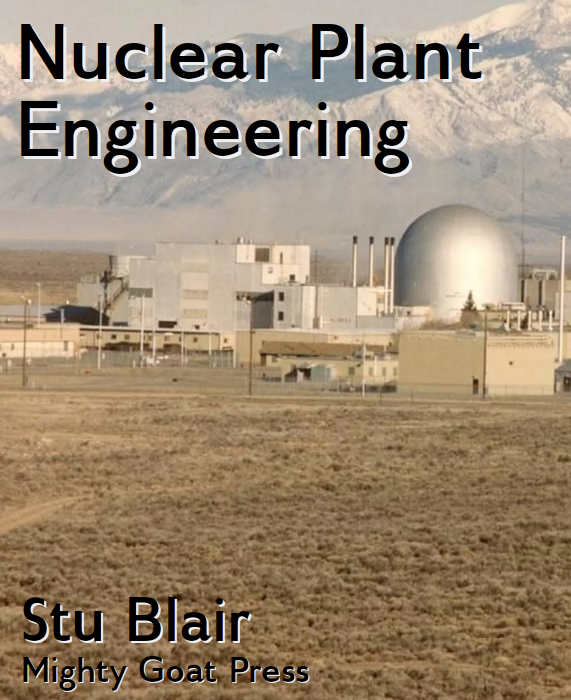
\includegraphics[width=1.5\textwidth]{cover5a.png}
\end{figure}
\end{fullwidth}

% Front matter
\frontmatter

% r.1 blank page
%\blankpage


% v.2 epigraphs
\newpage\thispagestyle{empty}
\vfill
%\openepigraph{
%A good mind may be compared to a vein of precious metal embedded in rock.  If it is to be of value, it %must first be recognized, then laboriously brought forth and carefully worked over.
%}%{H.G. Rickover}

\vfill
\openepigraph{%
...principles are more important than facts...
}{H.G. Rickover}


\vfill
\openepigraph{%
\ldots one of the prerequisites of originality is the art of forgetting, at the proper moment, what we know. Without this art the mind remains cluttered with ready-made answers and is not forced to ask the proper questions.
}{H.G. Rickover}


% r.3 full title page
\maketitle


% v.4 copyright page
\newpage
\begin{fullwidth}
~\vfill
\thispagestyle{empty}
\setlength{\parindent}{0pt}
\setlength{\parskip}{\baselineskip}
Copyright \copyright\ \the\year\ \thanklessauthor

\par\smallcaps{Published by \thanklesspublisher}

%\par\smallcaps{tufte-latex.github.io/tufte-latex/}
%
%\par Licensed under the Apache License, Version 2.0 (the ``License''); you may not
%use this file except in compliance with the License. You may obtain a copy
%of the License at \url{http://www.apache.org/licenses/LICENSE-2.0}. Unless
%required by applicable law or agreed to in writing, software distributed
%under the License is distributed on an \smallcaps{``AS IS'' BASIS, WITHOUT
%WARRANTIES OR CONDITIONS OF ANY KIND}, either express or implied. See the
%License for the specific language governing permissions and limitations
%under the License.\index{license}

\par\textit{First printing, \monthyear}
\end{fullwidth}

% r.5 contents
\tableofcontents

\listoffigures

\listoftables

% r.7 dedication
%\cleardoublepage
%~\vfill
%\begin{doublespace}
%\noindent\fontsize{18}{22}\selectfont\itshape
%\nohyphenation
%Dedicated to the midshipmen of the United States Naval Academy; the future of our armed services and of %our country.
%\end{doublespace}
%\vfill
%\vfill


% r.9 introduction
\cleardoublepage
\chapter*{Preface}

The goal of this book is to teach a selection of topics in energy conversion and thermal-hydraulics.  The book is organized into 30 lectures and is derived from notes developed for the course ER468 Nuclear Plant Engineering taught at the United States Naval Academy over a period spanning roughly from spring 2015 through the fall of 2022.

Students of this course are all expected to have taken courses in engineering thermodynamics and fluid dynamics; most students also take a course in heat transfer concurrently with ER468.  Consequently several introductory topics are skipped altogether.  The energy conversion topics---comprising extensive treatment of Rankine, Brayton, and combined cycles---omit treatment of the most fundamental topics of thermodynamics; the thermal-hydraulics lectures cover nuclear-specific extensions of fluid dynamics and heat transfer with only the briefest mention of introductory material.

The textbook used for the course while these lecture notes were prepared is Nuclear Systems by Neil Todreas and Mujid Kazimi.\cite{todreasNS}  Material from that excellent text is incorporated throughout these notes.

One unconventional aspect of this text is the extensive use of MATLAB\cite{matlab} for carrying out calculations.  Students of this course are expected to be familiar with the MATLAB programming environment and language features.  Thermal and transport properties of fluids are made available with the help of EasyProp,\cite{easyprop} which is a Python interface to the free and open-source library CoolProp and its associated Python wrapper.\cite{coolprop_wrapper} All of the examples provided in this  text use MATLAB but the underlying Python libraries could, of course, be used in Python. The goal of this approach is to make these material properties available in a computing environment that the students could easily use in conjunction with their other engineering analysis workflows; I specifically wanted to avoid a special-purpose tool that could only be employed separately.  

As with any textbook, the assignments comprise an essential element of the material presented.  The assignments presented in this text were delivered in a ``workshop'' format; the class met in a computer laboratory and students spent a class period working the problems.  This format provides ample opportunities for the students to ask questions---directed at the instructor or to each other---resulting in a very efficient learning environment.  However you go about it, you will miss out on a lot of material if you choose to skip the assignments.



%%
% Start the main matter (normal chapters)
\mainmatter

\part{Nuclear Energy Conversion}
\chapter{Lecture 1 - Course Introduction, Rankine Cycle Review}
\label{ch:lec1}%<< think of better label and chapter names
\section{Objectives}
The objectives of this lecture are:
\begin{itemize}
\item Introduce the course including basic topics covered, syllabus, and course policy
\item Review the basic Rankine Cycle that you learned in EM319 Thermodynamics I
\end{itemize}

\section{Course Introduction}
The basic topics that we will cover include:
\begin{enumerate}
\item Rankine Cycle 
\item Brayton Cycles
\item Combined Cycles 
\item Hydraulic analysis of nuclear systems
\item Thermal analysis of nuclear systems
\item Non-steady-state analysis 
\end{enumerate}
\newthought{The first three topics comprise} a thorough introduction to nuclear energy conversion.  The cycles that we analyze will range in complexity to allow introductory concepts to be reviewed while also addressing energy conversion cycles of practical relevance in modern nuclear systems; the latter are necessarily complex.

The last three topics are core elements of a typical ``thermal-hydraulics'' course and extend concepts taught in more general fluid dynamics and heat transfer classes with concepts and correlations that are relevant to nuclear applications.

%\subsection{Course Administrative Materials}
%The course syllabus and course policy statements are provided separately.
%
%\subsection{Course  Policy Highlights}
%The following elements of the course policy are highlighted here:
%\begin{itemize}
%\item There will be 3 mid-term exams each comprising 15\% of your final grade.  
%\item The final exam accounts for 30\% of your grade.
%\item Approximately 12 problem sets will be assigned, collectively comprising the %remaining 25\% of your grade.
%\marginnote{
%Summary of grade breakdown:
%\begin{enumerate}
%\item Midterm Exams (3) - 45\%
%\item Final Exam - 30\%
%\item Problem Sets - 25\%
%\end{enumerate}
%}
%\item Homework must be submitted on time.  Late homework will be assessed a 5\% %penalty for each calendar day past the due date.
%\item Attendance will be taken at the beginning of class.  You must be in your %seat and ready when attention is called; if you are not, you may be marked tardy %or absent.
%\end{itemize}
%Please do not hesitate to contact me if you have any questions or concerns %regarding these policy items.
%
\index{Rankine Cycle}
\section{Rankine Cycle Review}
\newthought{The overwhelming majority of} the energy conversion cycles for nuclear power plants are based on the Rankine Cycle. \marginnote{\emph{Rankine cycle} is another term for a "Steam Cycle" comprising a boiler or steam generator to make steam that is directed through a turbine that converts the thermal energy of the steam to mechanical work. The steam exiting the turbine is condensed to water and pumped back to the boiler or steam generator to complete the cycle.}  Features employed in various implementations of the Rankine cycle range from the compact, reliable, albeit \emph{simple} steam plants used on nuclear submarines to complex but highly efficient - and correspondingly difficult to analyze - systems used in commercial nuclear power plants.  In this course we will study Rankine cycles deeply.  As a starting point, however, we will use a simplified and idealized representation of a basic Rankine cycle based on the Westinghouse AP1000. \cite{westinghouse2011westinghouse}  A schematic of this cycle is given in Figure \ref{fig:simple_rankine}.

\newthought{The simple ideal} Rankine cycle comprises four basic processes:
\begin{enumerate}
\item $(1 \rightarrow 2)$ \textbf{isentropic compression} A feed pump is used to increase the pressure (flow energy) of the saturated liquid that exits the condenser.
\item $(2 \rightarrow 3)$ \textbf{isobaric heat addition} Feed enters the steam generator and, at constant pressure, is heated until it changes phase, exiting the steam generator as a saturated vapor.
\item $(3 \rightarrow 4)$ \textbf{isentropic expansion} High pressure saturated vapor is expanded in a turbine; converting its thermal energy into mechanical energy.  The exhaust gas is (usually) a saturated mixture.
\item $(4 \rightarrow 1)$ \textbf{isobaric heat rejection} The saturated mixture leaving the turbine exhausts into a condenser where, again at constant pressure, heat is rejected to condenser cooling water until the fluid is in a liquid state.
\end{enumerate}
The numbers in parenthesis correspond to state point labels provided in Figure \ref{fig:simple_rankine}.

\begin{figure}
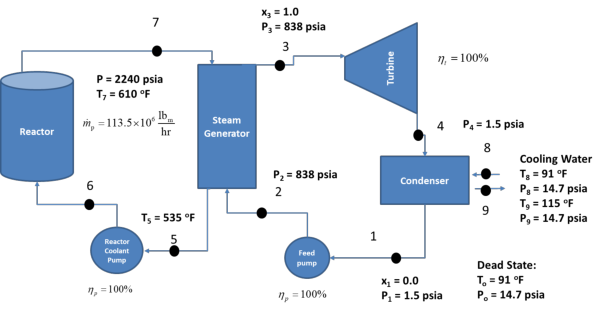
\includegraphics{simple_ideal_rankine.pdf}
\caption{Simple ideal Rankine cycle modeled on the Westinghouse AP1000.}
\label{fig:simple_rankine}
\end{figure}

It is also customary to illustrate the Rankine cycle on a Temperature-Entropy plot as shown in Figure \ref{fig:simple_rankine_TS}.  The numbers correspond to state-points, the curve is representative of the saturation curve for water.  The lines connecting the state point numbers represent the constant pressure or constant entropy contours, and the arrows and labels are indicating the transfer of heat and work to and from the cycle.

\begin{marginfigure}
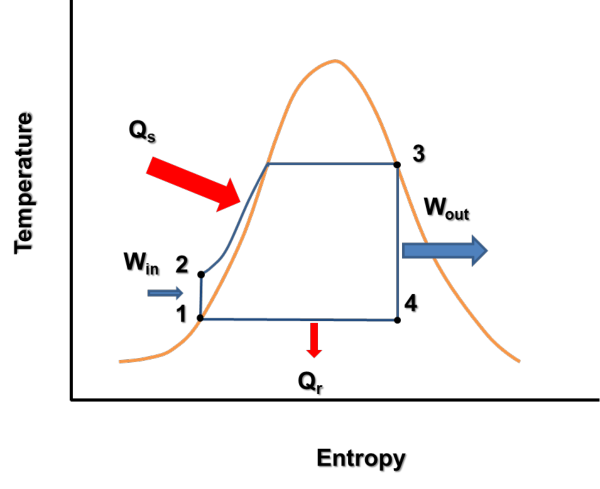
\includegraphics{simple_ideal_rankine_TS.pdf}
\caption{Temperature-Entropy plot of a simple, ideal, Rankine cycle.}
\label{fig:simple_rankine_TS}
\end{marginfigure}

\newthought{We will first analyze} this cycle from the perspective of conservation of energy.  Equation \ref{eq:sfee} captures the energy terms of relevance for this analysis.
\marginnote[1cm]{
Notes on Equation \ref{eq:sfee}:
\begin{itemize}
\item PE = potential energy
\item KE = kinetic energy
\item enthalpy is the sum of flow energy $(P\nu)$ and internal energy $(u)$.
\end{itemize}
}
\begin{equation}
q_{i \rightarrow f} - w_{i \rightarrow f}=\underbracket{\frac{g}{g_c}\left(z_f - z_i \right)}_{\Delta \text{PE}} + \underbracket{\frac{1}{2g_c}\left(v_f^2 - v_i^2\right)}_{\Delta \text{KE}} + \underbracket{\left(h_f - h_i\right)}_{\Delta \text{ enthalpy}}
\label{eq:sfee}
\end{equation}

For processes comprising energy conversion cycles in this course, we will assume that $\Delta$PE and $\Delta$KE are negligible unless specified otherwise.  Consequently we can generally simplify the conservation of energy equation as in Equation \ref{eq:sfee_simple}.

\begin{equation}
q_{i \rightarrow f} - w_{i \rightarrow f} = h_f - h_i
\label{eq:sfee_simple}
\end{equation} 

\newthought{Analyzing each process of } the simple ideal Rankine cycle for conservation of energy can be carried out for each process as:
\begin{itemize}
\item $(1 \rightarrow 2)$ , isentropic compression $\rightarrow q_{1 \rightarrow 2} = 0$\marginnote[-0.5cm]{\textbf{Reminder:} \emph{isentropic} processes are \emph{reversible} and \emph{adiabatic}.  When we say a process is \emph{adiabatic} that means no heat in or out of the process, and thus $q_{1 \rightarrow 2} = 0$ }.  $w_{1 \rightarrow 2} = h_1 - h_2$\marginnote[0.5cm]{\textbf{Question:} do you expect $w_{1 \rightarrow 2}$ to be positive or negative?}
\item $(2 \rightarrow 3)$, isobaric heat addition $\rightarrow w_{2 \rightarrow 3} = 0$. $q_{2 \rightarrow 3} = h_3 - h_2$
\item $(3 \rightarrow 4)$, isentropic expansion $\rightarrow w_{3 \rightarrow 4} = h_3 - h_4, \ q_{3 \rightarrow 4}=0$.
\item $(4 \rightarrow 1)$, isobaric heat rejection $\rightarrow q_{4 \rightarrow 1} = h_1 - h_4, \ w_{4 \rightarrow 1} = 0$.
\end{itemize}

We can compute the net specific work $(w_{\text{net}})$ and net specific heat $(q_{\text{net}})$\marginnote{\emph{Net specific work} is the amount of work produced per unit mass; \emph{net specific heat} is similarly defined.  In SI units both are typically given in kJ/kg; in USCS units: BTU/lbm.} by summing the corresponding terms from each process in the cycle.

\begin{equation*}
\begin{aligned}
q_{\text{net}} &=q_{2 \rightarrow 3}+q_{4 \rightarrow 1} &=h_3 - h_2 + h_1 - h_4 &= h_1+h_3 - (h_2+h_4)\\
w_{\text{net}} &=w_{1 \rightarrow 2}+w_{3 \rightarrow 4} &=h_1-h_2 + h_3 - h_4 &=h_1+h_3 - (h_2+h_4)
\end{aligned}
\end{equation*}
Comparing the equations above we can see that all of the same terms are listed in the right-most equality.  From this we get a fundamental result stemming from conservation of energy:

\begin{equation*}
w_{\text{net}}=q_{\text{net}}
\end{equation*}

When analyzing thermodynamic cycles you should\sidenote{You \emph{\textbf{must}}!!} always compute $w_{\text{net}}$ and $q_{\text{net}}$ and confirm that they are the same.  If they are not the same, your answer cannot be correct.\sidenote{Sadly, the converse is not true; if $w_{\text{net}}=q_{\text{net}}$, it is still possible that your answer is wrong.}

\newthought{In addition to computing net specific work} and net specific heat, we customarily compute the thermal efficiency $(\eta_{\text{TH}})$.  As you doubtless remember from your introductory thermodynamics class, the thermal efficiency is given by:
\index{efficiency, thermal}
\begin{equation}
\eta_{\text{TH}}=\frac{w_{\text{net}}}{q_{s}}
\label{eq:thermal_efficiency}
\end{equation}
Where $q_s$ is the specific heat supplied and, for this cycle, is equal to $q_{2\rightarrow 3}$.\marginnote[-1cm]{\textbf{Reminder:} the Rankine Cycle is an example of a \emph{heat engine}.  For heat engines, the basic deal is: you provide the heat, the heat engine converts the heat to work.  At best, you might hope that a really good heat engine would convert all of the heat to work; this would correspond to a thermal efficiency of 100 percent.  In other words: the thermal efficiency is the measure that tells you what fraction of the input heat gets converted into output work.  Unfortunately it is a practical fact, which we will discuss in future lectures, that the maximum thermal efficiency is limited to far less than 100 percent. }

\begin{example}
\textbf{Simple Ideal Rankine Cycle: }Consider a Rankine Cycle used for energy conversion for a nuclear power plant.  Saturated Steam is produced at a pressure of 838 psia and the condenser pressure is 1.5 psia.  Assume all components are ideal.  Using steam tables or a Mollier chart, estimate net work and thermal efficiency for this cycle.

\vspace{0.5cm}
\emph{Answers: $w_{\text{net}}$=390.3 BTU/lbm,  $\eta_{\text{TH}}=35.1\%$}
\end{example}



% want to manage chapters separately
% chapter = lecture
\chapter{Lecture 2 - Thermodynamic Analysis with EasyProp}
\label{ch:ch2}
\section{Objectives}
The objectives of this lecture are:
\begin{itemize}
\item Describe the EasyProp tools
\item Provide options for access to EasyProp
\item Do an Example Rankine cycle calculation with EasyProp
\end{itemize}

\section{The EasyProp Tools}

\begin{marginfigure}
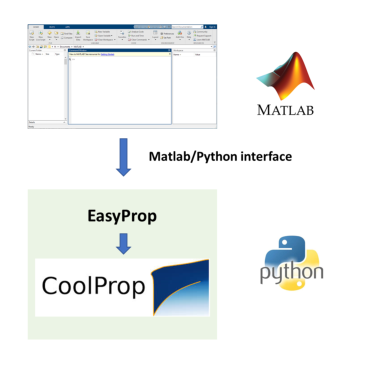
\includegraphics{Matlab-EasyProp-Schematic.pdf}
\caption{Schematic relationship between MATLAB and EasyProp}
\label{fig:matlab-easyprop}
\end{marginfigure}

What is EasyProp? \index{EasyProp}

\begin{itemize}
\item A library written in the Python language based on the free and open-source library CoolProp.  A schematic representation of the relationship between MATLAB, Python and the EasyProp and CoolProp Python libraries is given in Figure \ref{fig:matlab-easyprop}.
\item Accessible in a MATLAB environment with a properly initialized call to \emph{pyversion}\sidenote{The MATLAB function \emph{pyversion} sets several MATLAB environment variables that have the primary effect of ``telling'' MATLAB the path to the Python implementation that should be used when executing MATLAB scripts that use Python objects.}
\end{itemize}
How do I access EasyProp?

\begin{enumerate}
\item Login to \emph{ESSEX} via remote desktop and use any version of MATLAB installed
\begin{enumerate}
\item All software tools and libraries needed to use EasyProp have already been installed on this platform.
\item Users \emph{may} need to run \emph{pyversion\_fixer.m}\marginnote{The script \emph{pyversion\_fixer.m} will be made available to students as necessary.} to invoke the MATLAB built-in function \emph{pyversion} with the path to the local Python installation on \emph{ESSEX}.
\end{enumerate}
\end{enumerate}
Or
\begin{enumerate}[resume]
\item Install the required Python and MATLAB tools on your own laptop.
\begin{enumerate}
\item Download Anaconda (Anaconda3, Windows 64-bit, Python version 3.8) \marginnote[-2.25cm]{\textbf{Note: }If you opt for this method, you will have Python installed on your own laptop.  This is worthwhile.  When you graduate from USNA you will lose access to MATLAB along with many of the other non-free software packages that you may have become accustomed to using as a midshipman.  You can take Python with you and it can become the most powerful tool in your computational toolbox.}
\item From Anaconda prompt: conda install -c conda-forge coolprop
\item Locate Python executable.  One way to do this is from Anaconda prompt use the command: where python
\item In MATLAB call \emph{pyversion} with path to Python executable. E.g. >>pyversion('[path to python executable]')
\end{enumerate}
\end{enumerate}

\section{EasyProp Interface}
\newthought{A succinct introduction} to the EasyProp interface is available in the appendices.  For the remainder of this lecture I will try to exemplify the \emph{structure} of a MATLAB script in which EasyProp is being used.  I will follow this with a worked example where EasyProp is used to analyze a simple ideal Rankine Cycle.

\newthought{A basic analysis script} using EasyProp will flow as follows:

\begin{enumerate}
\item Ensure the Python system path includes the current directory 
\end{enumerate}


This is accomplished with the following code:\marginnote{Notice that we use the MATLAB commands 
\emph{clear}, \emph{clc}, and \emph{close 'all'}.  This is done in observation of the MATLAB Style requirement that we start every script with these three commands.  

MATLAB Style requirements are specified in the Appendix however I will use repetition in the lecture notes in an attempt to provide added emphasis.
}
\begin{lstlisting}[caption=Add the current directory to the Python system path, label={EP_setPath}]
%% Prepare the environment
clear;
clc;
close 'all';

EasyProp_path = ' '; %<- Path if EasyProp.py is in your current directory
if count(py.sys.path,EasyProp_path) == 0  % <-- see if desired directory is on path
    insert(py.sys.path,int32(0),EasyProp_path); %<-- if not; add it.
end
\end{lstlisting}

\begin{enumerate}[resume]
\item Construct a simple fluid object.
\end{enumerate}\marginnote{The leading \emph{py} tells MATLAB that what follows must be executed by the Python interpreter. The \emph{EasyProp} points to a particular Python library, and \emph{simpleFluid} is a function call within the EasyProp library.  The function \emph{simpleFluid} is a special type of function called a \emph{constructor}.}
\begin{lstlisting}[caption=Construct a \emph{simpleFluid} object]
units = 'USCS';
fluid = 'Water';
water = py.EasyProp.simpleFluid(fluid, units);
\end{lstlisting}
A list of common fluids that we will use in this course is provided in Table \ref{tab:fluid_list}.
\begin{margintable}
\begin{tabular}{cc}
\toprule
Fluid & EasyProp Name \\
\midrule
water & 'Water' \\
air & 'Air' \\
Carbon Dioxide & 'CO$_2$' \\
Nitrogen & 'N2' \\
Helium & 'He' \\
Refrigerant R245fa & 'R245fa' \\
\bottomrule
\end{tabular}
\caption{Commonly used EasyProp fluid designations}
\label{tab:fluid_list}
\end{margintable}

\begin{enumerate}[resume]
\item Establish problem parameters
\end{enumerate}

\begin{lstlisting}[caption=Set problem parameters]
numSp = 4; % number of state points
eta_turbine = 1.0; % isentropic efficiency of the turbine and pump
eta_pump  = 1.0;
Pmax = 838; % psia, max pressure
Pmin = 1.5; % psia, min pressure
\end{lstlisting}

\begin{enumerate}[resume]
\item Allocate fluid property arrays \marginnote{Pre-allocation of arrays is mandated in the ER468 style rules.  In this example we construct the arrays using the \emph{nan} function which, besides allocating memory for the arrays, initializes each value to ``Not-a-number'' (or \emph{nan}).  ``Not-a-number'' is preferred because it can never be mistaken for a number and thus can never be mistaken for a valid property value. This avoids the common logical error of using an array value with some incorrect-but-valid initial value (like zero).}  
\end{enumerate}

\begin{lstlisting}[caption=Allocate arrays to hold fluid property data.]
%% declare fluid property arrays
h = nan(numSp,1);
h_s = nan(numSp,1);
s = nan(numSp,1);
s_s = nan(numSp,1);
P = nan(numSp,1);
T = nan(numSp,1);
T_s = nan(numSp,1);
\end{lstlisting}

\begin{enumerate}[resume]
\item Determine fluid properties by using the functions associated with the EasyProp simpleFluid object.
\end{enumerate}

An example function call as follows: water.h\_pT(14.7,25)

\begin{equation*}
\underbracket{\text{water}}_{\text{object}}.\underbracket{\text{h\_pT}}_{\text{function}}\underbracket{\text{(14.7,25)}}_{\text{arguments}}
\end{equation*}

The "object" is the name of the Python object constructed in the step above.  The function name is given by convention;\marginnote[-3cm]{\textbf{Note: }Function name convention: [output property]\_[input property][input property](Arg 1, Arg 2).  In most cases the output thermodynamic property is determined based on two other known properties. In the case given, enthalpy (h) is determined as a function of pressure (p) and temperature (T)} in this case the property to be returned is the fluid enthalpy as a function of pressure and temperature.  The arguments - 14.7 and 25 - are the corresponding pressure and temperature; in this unit system they are given in units of psia and degrees Fahrenheit respectively.
\begin{margintable}
\begin{tabular}{lc}
\toprule
Property & EasyProp Abbreviation \\
\midrule
Pressure & p \\
Temperature & T \\
enthalpy & h \\
internal energy  & u \\
entropy & s \\
specific volume  & v \\
quality & x \\
viscosity & mu \\
\bottomrule
\end{tabular}
\caption{Property abbreviations}
\label{tab:property-list}
\vspace{0.5cm}
\end{margintable}

A list of fluid property abbreviations is given in Table \ref{tab:property-list}.  A list of units for each property used in the SI and USCS unit systems is given in Table \ref{tab:unit-list}.


\begin{margintable}
\begin{tabular}{lcc}
\toprule
Property & SI & USCS \\
\midrule
Temperature & C & F \\
Pressure & kPa & psia \\
enthalpy & kJ/kg & BTU/lbm \\
\bottomrule
\end{tabular}
\caption{EasyProp units}
\label{tab:unit-list}
\end{margintable}

\newthought{The remaining functions} needed to determine fluid properties at the state points are given in the listing below.

\begin{lstlisting}[caption=Find fluid properties for each state point in a simple Rankine cycle.]
%% calculate properties at state points 
% state point 1 - condenser outlet condensate pump inlet
P(1) = Pmin;
h(1) = myFluid.hL_p(P(1));
s(1) = myFluid.sL_p(P(1));

% compression from state point 1 to state point 2
P(2) = Pmax;
s_s(2) = s(1);
h_s(2) = myFluid.h_ps(P(2),s_s(2));
h(2) = h(1) - (h(1) - h_s(2))./eta_pump;

w_pump = h(1) - h(2);

% isobaric heat addition in the boiler from state point 2 to state point 3
P(3) = P(2);
h(3) = myFluid.hV_p(P(3));
s(3) = myFluid.sV_p(P(3));

q_s = h(3) - h(2);

% expansion in turbine from state point 3 to state point 4
P(4) = P(1);
s_s(4) = s(3);
h_s(4) = myFluid.h_ps(P(4),s_s(4));
h(4) = h(3) - eta_turbine*(h(3) - h_s(4));

w_turbine = h(3) - h(4);

% isobaric heat rejection in the condenser from sp 4 to sp 1
q_r = h(1) - h(4);
\end{lstlisting}

\begin{enumerate}[resume]
\item Complete analysis to find thermal efficiency and net work
\end{enumerate}
\begin{lstlisting}[caption=Analyze for net work and thermal efficiency]
%% First Law Check
w_net = w_pump + w_turbine;
q_net = q_s + q_r;

fprintf('Net work = %g kJ/kg \n',w_net);
fprintf('Net heat = %g kJ/kg \n',q_net);

%% Compute Thermal Efficiency
eta_th = w_net/q_s;

fprintf('Thermal efficieency = %4.1f percent \n',eta_th*100);
\end{lstlisting}

\newthought{There is more to analyze} than simply obtaining values for net specific work and thermal efficiency. Some fundamental things to think about:
\begin{enumerate}
\item Are my results correct?  In general it is difficult to know; most relevant problems do not come with a solution key.  You should take steps to increase your confidence that your answer is sensible.  A few essential steps include:
\begin{enumerate}
\item If you have computed net specific work, you should also compute net specific heat ($q_{net}$) and verify that they are, to within reasonable limits of precision, equal to each other. \sidenote[][-1cm]{When using a tool like EasyProp, $q_{net}$ and $w_{net}$ should be well within 1 BTU/lb$_{\text{m}}$ or 1 kJ/kg of each other.  If not, you probably have a bug somewhere.}
\item Is your computed thermal efficiency less than the Carnot efficiency?  If not: it is definitely wrong.
\item How does this answer compare to your results for a similar cycle?  Do the differences make sense? or
\item If you make small changes to the problem parameters---e.g. you slightly change the maximum/minimum system temperature/pressure---does that result in the expected change to net work and thermal efficiency?
\end{enumerate}
\item What are the strengths and weaknesses of the cycle that I have just analyzed? What could I change to make it better?  
\end{enumerate}
Answers to the question above cannot be given in general but you will become better at answering them with practice.  This course is designed to give you plenty of practice.




\chapter{Assignment \#1: Basic Rankine Cycles}
\label{ch:ass1}

Use MATLAB and EasyProp to answer the following questions
\begin{fullwidth}
\begin{enumerate}
\item Steam flowing at 15.9 lb$_{\text{m}}$/s enters the turbine of a simple Rankine cycle power plant at 1000 psia, 800$^{\circ}$F and exits at 2 psia.  Saturated liquid exits the condenser.  Assume that the turbine and pump are isentropic. (\textbf{Note:} 1 kW = 3412 BTU/hr, 1 hp = 2545 BTU/hr)
\begin{enumerate}
\item How many degrees superheat (degrees above saturation temperature) is the steam exiting the boiler?
\item What is the quality of the steam exiting the turbine?
\item Determine the power output of the turbine in kW and hp.
\item Determine the power input to the pump in hp.
\item Determine the cycle thermal efficiency.
\end{enumerate}

\vspace{1.0cm}

\item In a 2-MW (turbine power output) Rankine cycle, saturated vapor leaves the steam generator at 2 MPa and expands in the turbine to an outlet condition of 15 kPa, 94\% quality.  Saturated liquid leaves the condenser.  Assume the pump is isentropic.
\begin{enumerate}
\item What is the isentropic efficiency of the turbine?
\item Determine the flow rate fo the steam [kg/s].
\item Determine the cycle thermal efficiency.
\end{enumerate}

\vspace{1.0cm}
\item Investigate the effect of the condenser pressure on the performance of a simple ideal Rankine cycle.  Turbine inlet conditions of the steam are maintained constant at 5 MPa and 500$^{\circ}$C while the condenser pressure is varied from 5 to 100 kPa.  Determine the thermal efficiency of the cycle and plot it against the condenser pressure.  Write a short essay (no need to exceed 500 wrods) discussing the results.  Be sure to include a discussion on the extent to which the designer of an energy conversion system based on the Rankine Cycle has control of condenser pressure.

\end{enumerate}
\end{fullwidth}

\chapter{Lecture 3 - Carnot Cycle and Exergy Overview}
\label{ch:ch3}
\section{Objectives}
The objectives of this lecture are:
\begin{itemize}
\item Describe the Carnot Cycle
\item Review the Simple Ideal Rankine Cycle in context of a Carnot Cycle
\item Introduce exergy and provide related definitions.
\end{itemize}

\section{The Carnot Cycle}
\index{Carnot Cycle}
\newthought{The Carnot cycle is} an idealized heat engine that you should have learned about in a basic thermodynamics class or from a reference text.\cite{moran2010fundamentals}  It is idealized in the sense that it represents the most efficient possible heat engine working between two (high and low temperature) thermal reservoirs.  A temperature-entropy plot of the cycle is shown in figure \ref{fig:CarnotCycle} and consists of four processes:

\begin{marginfigure}
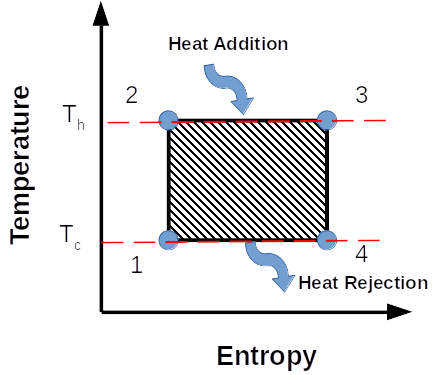
\includegraphics{Carnot_cycle_sketch.png}
\caption{Temperature-Entropy plot of a Carnot cycle.}
\label{fig:CarnotCycle}
\end{marginfigure}

\begin{enumerate}
\item isentropic compression $1 \rightarrow 2$
\item isothermal heat addition $2 \rightarrow 3$
\item isentropic expansion $3 \rightarrow 4$
\item isothermal heat rejection $4 \rightarrow 1$

\end{enumerate}

The thermal efficiency of this cycle can be shown to be a function of the absolute temperature of the high temperature reservoir $\left(T_h\right)$ and the absolute temperature of the low temperature reservoir $\left(T_c\right)$.  

$$ \eta_{\text{Carnot}} = 1 - \frac{T_c}{T_h}$$ \index{efficiency, Carnot}

Note that as $T_c$ decreases or as $T_h$ increases, the Carnot efficiency increases.  Since both reservoir absolute temperatures are non-negative, and $T_h > T_c$, the Carnot efficiency can be no greater than 1 and achieves that only for $T_c=0$ or as $T_h \rightarrow \infty$.  

\newthought{The following concepts} should be emphasized:
\begin{enumerate}
\item No heat engine can convert all heat input to work; and
\item A Carnot cycle is a heat engine that produces the maximum possible efficiency for any heat engine operating between a given fixed hot and cold temperature reservoir.
\end{enumerate}

All of the processes of the Carnot Cycle are reversible and the work-in and work-out of process 1 and 3 are isentropic.  The heat-in and heat-out of process 2 and 4 are reversible because the heat is transferred isothermally.\marginnote[-4cm]{\textbf{Note: }It is not evident from the temperature-entropy diagram, but the isothermal heat transfer processes in a Carnot cycle also must take place across an infinitesimal temperature gradient.  We know from the laws of heat transfer that heat flows from high temperature to low temperature and the rate of heat transfer is proportional to:
\begin{enumerate}
\item the size of the heat transfer surface, 
\item the temperature difference, and 
\item some material property characterizing how ``well'' heat is transferred.  
\end{enumerate}
In order to transfer energy across an infinitesimal temperature gradient, the material must have arbitrarily good heat transfer properties, or the heat transfer surface must be arbitrarily large.  We will dismiss these practical complications for the time being and simply move forward. }

\section{Simple Ideal Rankine Cycle - Revisited}
\newthought{Consider again the} Simple Ideal Rankine cycle operating between the maximum pressure of 838 psia and minimum pressure of 1.5 psia.  A schematic temperature-entropy diagram of this process is shown below.

\begin{figure}
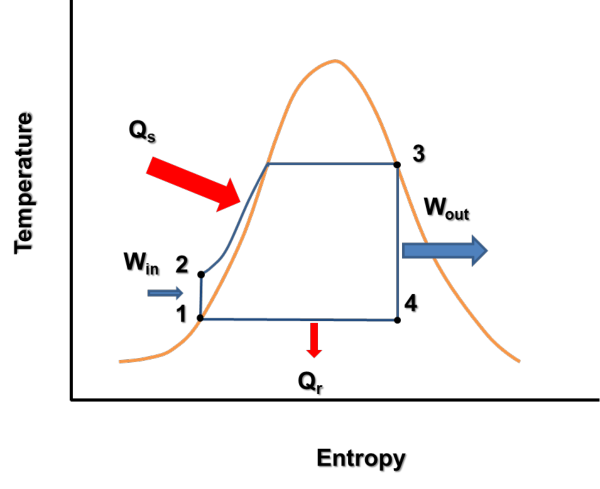
\includegraphics{simple_ideal_rankine_TS.pdf}
\caption{Temperature-Entropy plot of a simple, ideal, Rankine cycle.}
\label{fig:simple_rankine_TS_2}
\end{figure} 

From the example in Lecture 1, we know that the thermal efficiency is 35.1 percent and the net specific work is 390.3 BTU/lbm.  What is the Carnot efficiency of this cycle?
\begin{itemize}
\item To calculate the Carnot efficiency, we need the temperature of the hot and cold reservoirs respectively.
\item If we take $T_h$ to be the saturation temperature at 838 psia, we find that it is approximately 524 $^{\circ}$F; this corresponds to 984 R.\sidenote{If we're analyzing an AP1000 PWR energy conversion cycle, a better choice for $T_h$ would be the hot-leg temperature which is approximately 610 $^{\circ}$F.  We will come back to this in a future lecture.} 
\item If we take $T_c$ to be the condenser temperature (for heat rejection from state point 4 to 1), which is equal to the saturation pressure at 1.5 psia, we find that it is approximately 116 $^{\circ}$F; this corresponds to 576 R.\sidenote{Again, a better choice for $T_c$ for the AP1000 would be the inlet temperature of cooling water to the condenser which we might conservatively take to be 91 $^{\circ}$F.}
\item Thus the Carnot efficiency is: $\eta_{\text{C}} = 1 - \sfrac{576}{984} = 0.415$; or 41.5 percent.  
\end{itemize}

Consider the heat addition $(Q_s)$ from state points 2 to 3; unlike the Carnot cycle, the heat transfer does not occur isothermally.  Significant irreversibilities exist in this process.  Although the heat rejected in the process from state point 4 to 1 does occur at constant temperature, in practice the heat is rejected to an external heat sink across a finite temperature difference. This also is a source of irreversibility although it is not evident from the temperature-entropy diagram.  

\newthought{Suppose we modified} the Rankine Cycle above to make it \emph{more like} a Carnot cycle.  We could reject heat only to state point 1' in Figure \ref{fig:simple_rankine_TS_carnot} and apply work to isentropically compress the mixture until it became a saturated liquid at 838 psia, state point 2'.  What would the thermal efficiency be for that cycle?

\begin{marginfigure}
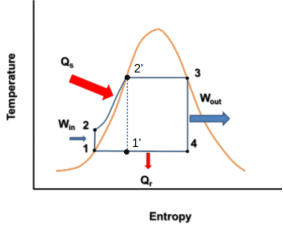
\includegraphics{simple_ideal_rankine_TS_carnot.pdf}
\caption{Temperature-Entropy plot of a modified Rankine cycle.}
\label{fig:simple_rankine_TS_carnot}
\end{marginfigure} 

The answer is 41.5 percent just like the Carnot cycle.  You would also find that the net specific work for the cycle is somewhat reduced.  Is that what you expect?  Again, the answer should be ``yes''; by changing state points 1 and 2 we reduced the area contained within the T-S diagram and that corresponds with reduced net specific work.

\index{Exergy}
\section{Exergy Analysis - Basic Definitions}
In order to analyze quantitatively the extent to which a cycle has reversibility we will need to perform an \emph{Exergy Analysis}.\marginnote{The course textbook does an \emph{irreversibility} analysis which is equivalent.}

\subsection{Definitions}
The following definitions are provided below:
\begin{itemize}
\item \emph{Exergy} is the maximum theoretically obtainable work that can be extracted from a working fluid as it comes into equilibrium with the environment.\marginnote[-1.5cm]{\textbf{Note: } exergy is defined for a working fluid only \emph{relative} to the environment.  Working fluid of a given state will have a different exergy if environmental temperature or pressure goes up or down.}

\index{Dead state}
\item \emph{Dead state} is a state in which a working fluid is at rest relative to the environment.  The dead state will normally be characterized by dead state temperature $(T_o)$ and dead state pressure $(P_o)$.

\index{Exergy, specific flow}
\item \emph{Specific Flow Exergy} ($e_f$) is an intrinsic thermodynamic variable quantifying the ability of a working fluid to do work.  It is calculated relative to the dead state as follows:
$$e_f = h - h_o - T_o(s - s_o) + \frac{V^2}{2} + gz$$
where $h$ and $s$ are the enthalpy and entropy of the working fluid; $h_o$ and $s_o$ are the enthalpy and entropy at the dead state temperature and pressure; $T_o$ is the dead state temperature; and $\sfrac{V^2}{2}$ and $gz$ represent the kinetic and potential energy respectively of the fluid.\sidenote{Unless otherwise noted, changes in kinetic and potential energy will be neglected in this class so, for calculations of $e_f$, those terms are excluded.}

\end{itemize}

\index{Exergy Balance}
\subsection{Exergy Balance}
\newthought{Unlike energy,} exergy is not conserved.  One can think of exergy like energy: we pass exergy in from a high energy source like the primary coolant of a PWR; we convert some of that exergy to work and some that is left over we have to reject to the environment.  But unlike energy, exergy can be destroyed. Exergy can also be lost through other means like heat transfer to the surrounding medium.\sidenote[][-1cm]{For example: steam piping passing through the engineroom of a submarine is hot; despite its lagging, it transfers some energy to the surrounding environment.  This is a loss of exergy that can be taken into account.}

We want to account for exergy in much the same way that we account for energy.  In words, this accounting balance looks like this:

$$\text{Exergy in} - \text{Exergy out} = \text{Exergy xfer by heat} + \text{Exergy xfer by work} + \text{Exergy Destroyed}$$

In equation form this translates as follows:

$$\sum_i \dot{m}_i e_{f_i} - \sum_e \dot{m}_e e_{f_e} = \sum_j \left(1-\frac{T_o}{T_j} \right)\dot{Q_j}+\dot{W} + \dot{E}_d$$
The terms are interpreted as follows:
\begin{itemize}
\item $\sum_i\dot{m}_i e_{f_i}$ is the sum of all flow exergy going \emph{in} to a particular process.  The variable $i$ corresponds to all of the inflows; $\dot{m}_i$ is the mass flow rate for each in-flow and $e_{f_i}$ is the specific flow exergy for each inflow.
\item $\sum_e \dot{m}_e e_{f_e}$ has the same meaning but for all flows \emph{exiting} a particular process.
\item $\sum_j \left(1-\sfrac{T_o}{T_j} \right)\dot{Q_j}$ is exergy transfer through heat. The variable $j$ enumerates all of the exit points for exergy transfer through heat for the system. $\dot{Q}_j$ is the corresponding rate of heat loss, $T_j$ is the temperature at which this heat is lost, and $T_o$ is the dead state temperature.
\item $\dot{W}$ is the rate of exergy transfer through work.  Any process that does work (e.g. turbine, pump, compressor) transfers exergy out of (turbine) or into (pump or compressor) the working fluid.
\item $\dot{E}_d$ is the rate of exergy destruction.  This should be interpreted as the rate at which exergy is lost due to irreversibilities.  Any non-reversible process will have positive exergy destruction.\sidenote{Exergy destruction rate for a process should \emph{never} be negative.  If your calculations show a negative exergy destruction rate (other than rounding errors near zero) for any process you have somehow violated the Second Law of Thermodynamics.  You need to stop and find the error before moving forward.}
\end{itemize}





\chapter{Lecture 4 - Rankine Cycle Exergy Accounting}
\label{ch:ch4}
\section{Objectives}
The objectives of this lecture are:
\begin{itemize}
\item Illustrate exergy accounting with a simple Rankine cycle
\item Show how to carry out the calculations in a MATLAB environment using EasyProp.
\end{itemize}

\section{Simple Ideal Rankine Cycle - Exergy Accounting}
\newthought{Consider again} the Rankine cycle with system parameters specified to resemble a highly simplified version of a Westinghouse AP1000. A schematic of this system is given in Figure \ref{fig:simple_rankine_3}.
\begin{figure}
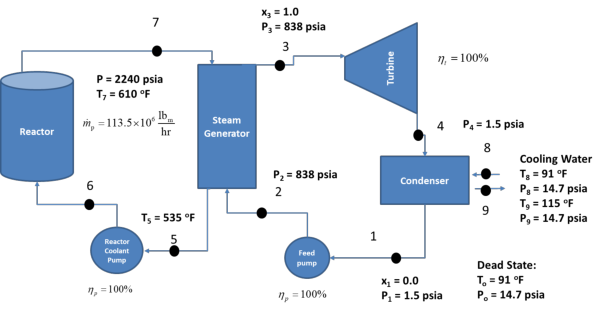
\includegraphics{simple_ideal_rankine.pdf}
\caption{Simple ideal Rankine cycle modeled on the Westinghouse AP1000.}
\label{fig:simple_rankine_3}
\end{figure}
Our goal is to carry out the exergy accounting as described in Lecture 3 for this system.  

\newthought{We will follow} a step-by-step process to complete this analysis.

\begin{enumerate}
\item Carry out the basic ``First Law'' of thermodynamics analysis for this system.  This was done in Lecture 2; the details will not be repeated here except to remind you that we have instantiated an object to calculate thermodynamic properties of the working fluid, water:

\begin{lstlisting}[caption=Construct a \emph{simpleFluid} object]
units = 'USCS';
fluid = 'Water';
water = py.EasyProp.simpleFluid(fluid, units);
\end{lstlisting}

\item Determine dead state enthalpy ($h_o$) and entropy ($s_o$).  With the given dead state temperature and pressure, we can find this as follows:
\begin{lstlisting}[caption=Find dead state enthalpy and entropy]
To_F = 91; % F, dead state temp
Po = 14.7; % psia, dead state pressure
ho = water.h_pT(Po,To_F);
so = water.s_pT(Po,To_F);
To = To_F + 460; % R, dead state absolute temperature
\end{lstlisting}
Note that EasyProp functions require the temperature in either C or F, but the $T_o$ appearing in the specific flow exergy equations must be in absolute units: K or R.
%\begin{marginfigure}
%
\includegraphics{bug-icon.png}
%\end{marginfigure}

\item Calculate the specific flow exergy for all state points.  You should calculate all state point enthalpy and entropy values as part of your ``First Law'' analysis.  In MATLAB one can then create an in-line function to quickly calculate the specific flow exergy for all state points.

\begin{lstlisting}[caption=Compute specific flow exergy for all state points]
ef_fun = @(h,s) (h - ho) - To*(s - so);
ef = ef_fun(h,s); % BTU/lbm, specific flow exergy 
\end{lstlisting}
Note that the arrays for $h$ and $s$ should be populated with the correct enthalpy and entropy for all state points before this calculation is made.
\item Calculate the exergy destruction rate for each process.  In each process this is calculated from a re-arrangement of the exergy balance equation given in Lecture 3:

\begin{equation}
\dot{E}_d = \sum_{i}\dot{m}_i e_{f_i} - \sum_{e} \dot{m}_e e_{f_e} - \dot{W}
\label{eq:ex_d_eqn}
\end{equation}

In this cycle there are four processes to consider:
\begin{enumerate}
\item \textbf{Exergy destruction rate in the steam generator.}  Focus on the relevant process showing in Figure \ref{fig:SIR_sg}.  The steam generator has two in-flows and two exits; one each from the primary and secondary side.  For this particular problem we are only given the mass flow rate of the primary ($\dot{m}_p$) so we first need to get the mass flow rate in the secondary.  This can be obtained from simple conservation of energy principles:
$$ \dot{m}_s(h_3 - h_2) = \dot{m}_p(h_7 - h_5)$$

\begin{marginfigure}
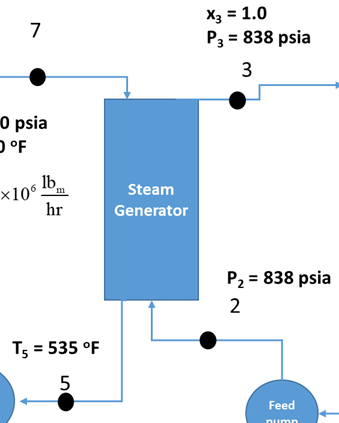
\includegraphics{SIR_sg.png}
\caption{Constant pressure heat transfer process in the steam generator}
\label{fig:SIR_sg}
\end{marginfigure}
\begin{lstlisting}
m_s = m_p*(h_7 - h_6)/(h_3 - h_2); % lbm/hr, mass flow rate through S/G.
\end{lstlisting}
Now, using Equation \ref{eq:ex_d_eqn}, we compute the exergy destruction rate:

\begin{lstlisting}
Ex_d_sg = m_p*ef(7) + m_s*ef(2) - (m_p*ef(5) + m_s*ef(3)); % BTU/hr
\end{lstlisting}
Note that since there is no work done in the steam generator, there is no exergy transfer through work.

\item \textbf{Exergy destruction rate in the turbine.} The relevant process here is shown in Figure \ref{fig:SIR_turb}.  Note that since there is work being done in the turbine, there is exergy transfer through work that we need to take into account.
\begin{marginfigure}
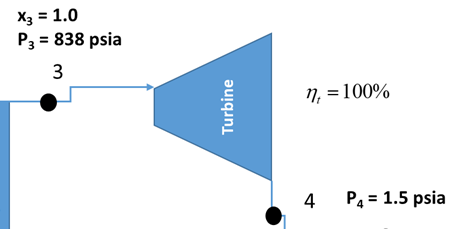
\includegraphics{SIR_turb.png}
\caption{Expansion of the working fluid in the turbine.}
\label{fig:SIR_turb}
\end{marginfigure}
\begin{lstlisting}
Ex_d_turb = m_s*(ef(3) - ef(4)) - m_s*w_turb; % BTU/hr 
\end{lstlisting}
Here we expect $w_{turb}$, the specific work of the turbine, to have previously been calculated in the ``First Law'' analysis as $w_{turb} = h(3) - h(4)$.\sidenote[][-1.25cm]{\textbf{Note: }for this simple ideal cycle, you should find that the exergy destruction rate for the ideal turbine to be zero!}

\item \textbf{Exergy destruction rate in the condenser.}  Analysis of the condenser is much like the steam generator: two in-flows and two exit-flows and no work done in the process.  Also in this case, like the steam generator, we need to use conservation of energy to determine the required flow rate of the condenser cooling water $\dot{m}_c$.  The relevant process schematic is illustrated in Figure \ref{fig:SIR_cond}.

\begin{marginfigure}
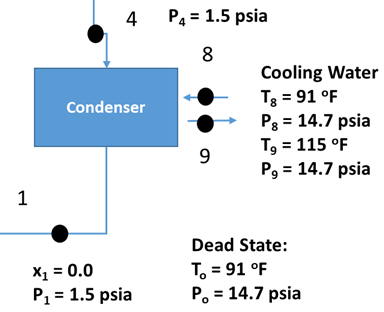
\includegraphics{SIR_cond.png}
\caption{Constant pressure heat rejection in the condenser.}
\label{fig:SIR_cond}
\end{marginfigure}

\begin{lstlisting}
m_c = m_s*(h(4) - h(1))/(h(9)-h(8)); % lbm/hr, condenser cooling water flow

Ex_d_cnd = m_c*ef(8) + m_s*ef(4) - (m_c*ef(9) + m_s*ef(1)); % BTU/hr
\end{lstlisting}

\item Exergy destruction rate in the feed pump.  Like the turbine, the feed pump has one inlet and one exit and there is also exergy transfer through work. The relevant process schematic is illustrated in Figure \ref{fig:SIR_mfp}. The MATLAB code would be:
\begin{marginfigure}
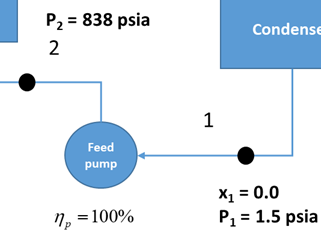
\includegraphics{SIR_mfp.png}
\caption{Work in to the working fluid from the feed pump.}
\label{fig:SIR_mfp}
\end{marginfigure}
\begin{lstlisting}
Ex_d_fp = m_s*(ef(1) - ef(2)) - m_s*w_fp; % BTU/hr
\end{lstlisting}
where $w_{fp}$ would be calculated simply as $w_{fp} = h(1) - h(2)$.  

\end{enumerate}

\item Calculate the ``Exergy In'' to the system from the primary coolant and ``Exergy Out'' from the system to the environment via the condenser.  For the Exergy In we will simply use the mass flow rate of primary coolant times the change in specific flow exergy of the primary coolant through the steam generator; for Exergy Out we will use the mass flow rate of condenser cooling water times the increase in specific flow exergy of the water.

\begin{lstlisting}
Ex_in = m_p*(ef(7) - ef(6)); % BTU/lbm
Ex_out = m_c*(ef(9) - ef(8)); % BTU/lbm
\end{lstlisting}

\item Verify the overall exergy balance.  The balance should look something like:

\begin{lstlisting}
balance = Ex_in - Ex_out - m_s*w_net - ...
          (Ex_d_sg + Ex_d_cnd + Ex_d_turb + Ex_d_fp);
\end{lstlisting}

\end{enumerate}

If everything is correct and if you have not violated the Second Law of Thermodynamics the computed balance should be zero.  In exactly the same way that you should verify that net specific work is the same as net specific heat transferred ($w_{net} = q_{net}$) --- thereby satisfying conservation of energy (First Law of Thermodynamics) --- you should check the balance on the exergy analysis to ensure you have satisfied the Second Law of Thermodynamics.


\chapter{Assignment \#2: Rankine Cycle 2nd Law Analysis}
\label{ch:ass2}

\section{Background}
Russia has recently placed a nuclear powered barge into operation named the \emph{Akademik Lomonosov.}  This vessel is not self-propelled but is equipped with two pressurized water reactors designated as KLT-40S for providing up to 35 MW of electrical power (each).

We will model the power conversion system for the KLT-40S as a simple Rankine Cycle with a Steam Generator (SG), a Turbine Generator (TG), a condenser and a main feed pump (MFP).  Thermal energy is supplied by primary coolant of a pressurized water reactor (PWR); waste heat is rejected to seawater which is modeled as ordinary water.  Relevant design parameters are given in Table \ref{tab:ass2}
\begin{table}
\begin{tabular}{l c}
\toprule
Parameter & Value \\
\midrule
Primary coolant pressure & 12.7 MPa \\
Primary coolant SG inlet temperature & 317$^{\circ}$C \\
Primary coolant SG outlet temperature & 280$^{\circ}$C \\
SG pressure & 3.8 MPa \\
SG steam outlet temperature & 290$^{\circ}$C \\
Steam mass flow rate & 67 kg/s \\
Dead state temperature and pressure & 5$^{\circ}$C, 101 kPa \\
Condenser pressure & 5 kPa\\
Consenser seawater inlet temperature & 5$^{\circ}$C \\
Seawater cooling temperature rise & 10$^{\circ}$C \\
MFP isentropic efficiency & 65\% \\
TG steam outlet quality & 80\% \\
\bottomrule
\end{tabular}
\caption{\emph{Akademic Lomonosov} Nuclear Steam Supply System key parameters.}
\label{tab:ass2}
\end{table}

\newthought{Analyze the }Rankine cycle described and answer the following questions:
\begin{fullwidth}
\begin{enumerate}
\item What is the isentropic efficiency of the TG?
\vspace{1.0cm}
\item What is the net specific work of the Rankine cycle? [kJ/kg]
\vspace{1.0cm}
\item Verify that the net specific heat is the same as the net specific work.
\vspace{1.0cm}
\item What is the mass flow rate of the primary coolant? [kg/s]
\vspace{1.0cm}
\item What is the mass flow rate of the condenser cooling water? [kg/s]
\vspace{1.0cm}
\item What is the rate of exergy input (to the Rankine cycle) from the primary coolant? [kW]
\vspace{1.0cm}
\item What is the rate of exergy rejection to the environment via condenser cooling water? [kW]
\vspace{1.0cm}
\item Compute the rate of exergy destruction in the Rankine cycle components; fill in the table below:
\begin{table}
\begin{tabular}{l | l}
\toprule
\textbf{Component} & \textbf{Rate of Exergy Destruction [kW]} \\
\hline
Steam generator &  \\
\hline
Turbine generator & \\
\hline
Condenser & \\
\hline
Main feed pump & \\
\hline
\hline
Total Exergy Destruction Rate & \\
\bottomrule
\end{tabular}
\end{table}

\vspace{1.0cm} 

\item What is the rate of exergy transfer through work? [kW]

\vspace{1.0cm}

\item Verify the 2nd law of thermodynamic balance:
$$\text{Exergy in - Exergy out } = \dot{W} + \dot{E}_{d}$$


\end{enumerate}
\end{fullwidth}

\chapter{Lecture 5 - Improving Rankine Cycle Performance}
\label{ch:ch5}
\section{Objectives}
The objectives of this lecture are:
\begin{itemize}
\item Describe performance parameters for Rankine Cycles
\item Illustrate benefits of Rankine Cycle with a Moisture Separator and Open Feedwater Heater
\item Show how adding a Reheater improves Performance
\item Include modeling details essential for cycle analysis
\end{itemize}

\section{Performance Changes with Increasing Steam Generator Pressure}

\newthought{Based on} our discussion from last lecture, it seems obvious enough that one way to improve Carnot efficiency and thus (hopefully!) increasing Rankine cycle performance would be to increase the steam generator temperature.  Since the steam generator is a saturated system, such a change implies an increase to steam generator pressure.  Let us assume for the time being that nothing limits us from increasing steam generator temperature and pressure; what are the thermodynamic consequences?  To start, let us examine the change on a temperature-entropy plot as is shown in Figure \ref{fig:T_S_increase_P}.

\begin{marginfigure}
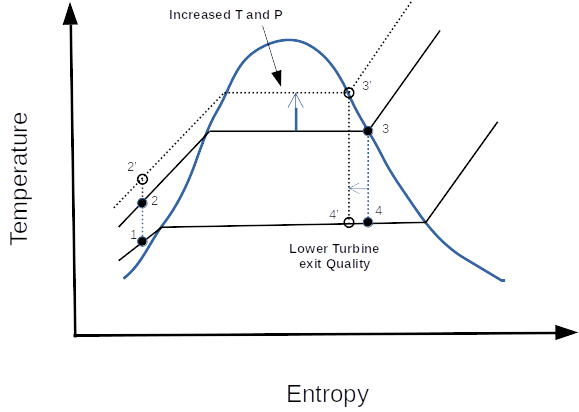
\includegraphics{T_S_increase_P.png}
\caption{Temperature Entropy plot showing an increase in steam generator pressure.}
\label{fig:T_S_increase_P}
\end{marginfigure}

\newthought{A few things} are apparent from this picture:
\begin{enumerate}
\item Since the temperature at which the majority of heat has been added to the system is increased, Carnot efficiency will increase and, all things being equal, the thermal efficiency that we actually achieve will also increase.
\item While the schematic is not drawn to scale, it suggests that net specific work will also increase at least a little. 
\item The turbine exit quality decreases after we increase the steam generator pressure.   

\end{enumerate}
The last two points on the above list might be clarified with a temperature-entropy plot that is drawn to scale.  Such a plot can be made with EasyProp tools and is shown in Figure \ref{fig:T_S_increase_P_toScale}.

\begin{marginfigure}
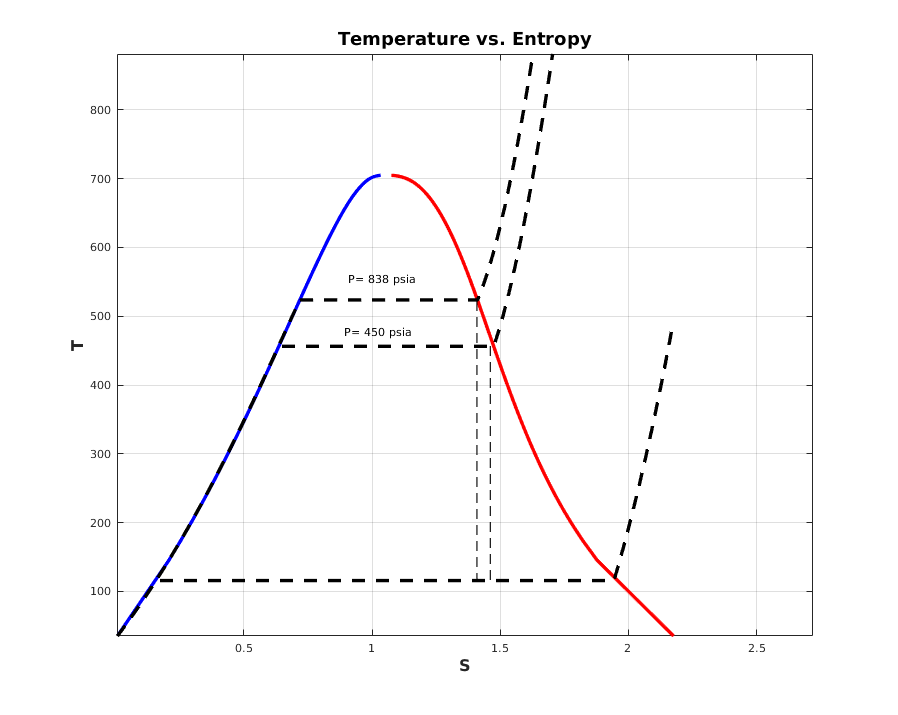
\includegraphics{TS_Pressure_Change_toScale_mf.png}
\caption{Temperature Entropy plot for steam pressure increase drawn to scale with EasyProp.}
\label{fig:T_S_increase_P_toScale}
\end{marginfigure} 

\newthought{Increasing efficiency is} a good goal but, in this case, the attendant reduction in turbine exit quality is a significant issue.  Droplets of saturated vapor in the steam can result in excessive turbine wear and reduces turbine isentropic efficiency.  The good news is that we can make changes to the cycle that address the issue with turbine exit quality while further increasing cycle thermal efficiency.

\index{Rankine Cycle, open feedwater heater}
\index{Rankine Cycle, moisture separator}
\section{Rankine Cycle with Moisture Separator and Open Feedwater Heater}
We can increase steam quality at the low-pressure stages of the turbines if, part way through the expansion process, we include a component that separates saturated liquid from the working fluid.  Such an apparatus is called a Moisture Separator (M/S) and is shown in the cycle schematic in Figure \ref{fig:RS_MS_OFWH}.

\begin{figure}
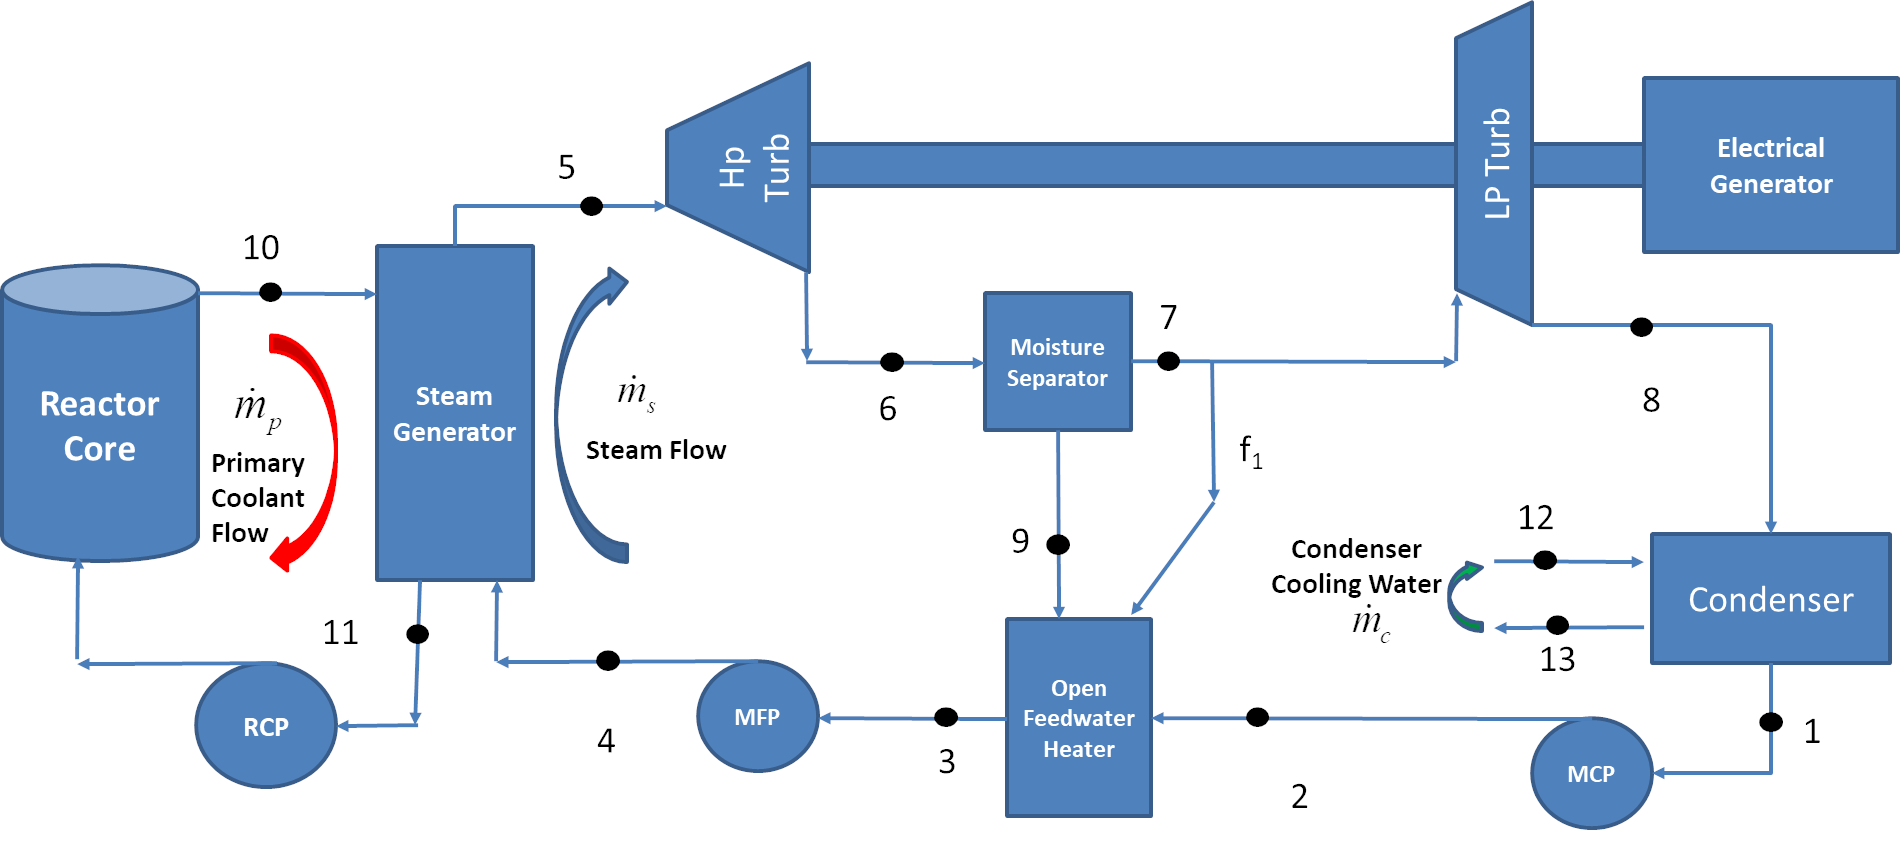
\includegraphics{Rankine_with_MS_and_OFWH.png}
\caption{Rankine Cycle with moisture separator and open feedwater heater.}
\label{fig:RS_MS_OFWH}
\end{figure} 

The moisture separator takes steam exiting the high pressure (HP) turbine at state point 6 which is a saturated mixture.  The portion of the steam that is saturated vapor\sidenote[][-1.0cm]{This fraction is easily obtained as the quality at state point 6, $x(6)$, using EasyProp.} exits the moisture separator to state point 7.  The portion of the steam that is saturated liquid\sidenote[][0cm]{Again, this can be found as the complement of quality at state point 6.} is drained to the Open Feedwater Heater (OFWH).\marginnote[1.25cm]{\textbf{Note: }The OFWH is ``open'' because all fluids flowing into the tank mix freely.  This has the added consequence that all fluid streams going into or out of the OFWH must be maintained at the same pressure.}

\newthought{There are three} streams going into the OFWH: discharge of the main condensate pump (state point 2); saturated liquid draining from the M/S (state point 9); and additional saturated vapor extracted from the steam flow path at the steam exit from the M/S (state point 7).  This last flow extraction is used to further pre-heat the feedwater in the OFWH.  Conventionally we set the extraction steam flow fraction ($f$) such that the fluid exiting the OFWH at state point 3 is near its saturation temperature.\sidenote[][-0.5cm]{We will adopt the modeling convention that the fraction $f$ extracted from the steam flow is set so the outflow from the OFWH is a saturated liquid.}

\newthought{The temperature-entropy plot} for this modified cycle is shown in Figure \ref{fig:TS_MS_OFWH}.  This illustrates how, at least, the problem of turbine exit quality is addressed.
\begin{marginfigure}
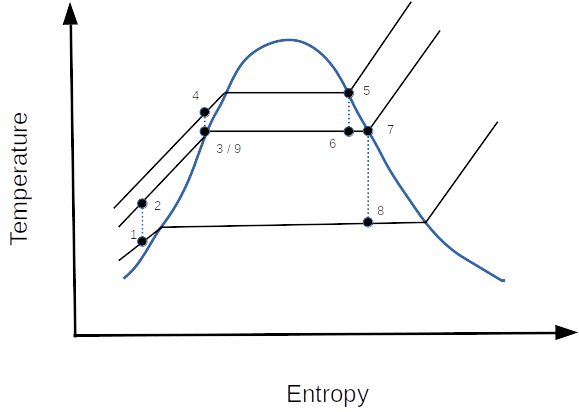
\includegraphics{TS_MS_OFWH.png}
\caption{Temperature-entropy plot of Rankine cycle with M/S and OFWH.}
\label{fig:TS_MS_OFWH}
\end{marginfigure}
One thing the figure does not show quantitatively is that the regeneration effect of pre-heating the feedwater in the OFWH has the result of increasing plant thermal efficiency.  This benefit comes at the cost of another effect that the temperature-entropy plot fails to highlight; the mass flow rate of steam through the low-pressure (LP) turbine is reduced thereby lowering specific work output from the cycle.

\subsection{``First Law'' Analysis of Modified Cycle}

\newthought{The analysis of this cycle} requires some modifications.  The reason for this is, owing to the separation of vapor and liquid in the M/S, the working fluid has different mass flow rates at different portions of the system.  For example, for a given mass flow rate through the S/G ($\dot{m}_{s}$), then the mass flow rate of steam exiting the M/S at state point 7 is $\dot{m}_s x(6)$, where $x(6)$ is the quality at state point 6.\sidenote{For this cycle where saturated vapor (x=1) is introduced into the HP turbine, $x(6)$ is generally less than 1.} Before the steam enters the LP turbine, the flow rate is further reduced since a fraction $f$ is directed to the OFWH for regeneration.  Thus the mass flow rate of steam entering the LP turbine is: $\dot{m}_s x(6)(1-f)$.

\newthought{As a convention} we will re-define ``specific work'' of a component ($w$) to be equal to the power from a component ($\dot{W}$) divided by the mass flow rate through the steam generator ($\dot{m}_s$).  See the examples below.


\begin{itemize}
%\begin{example}
\item \textbf{Example:} the specific work of the HP turbine ($w_{\text{HP}}$) is given by:
$$ w_{\text{HP}}= \frac{\dot{m}_s(h(5)-h(6))}{\dot{m}_s} = h(5) - h(6)$$
which happens to be no different than what we would have calculated before.
%\end{example}

%\begin{example}
\item \textbf{Example:} the specific work of the LP turbine ($w_{\text{LP}}$) is given by:
$$ w_{\text{LP}}= \frac{\dot{m}_s x(6) (1-f) (h(7) - h(8))}{\dot{m}_s} = x(6) (1-f) (h(7)-h(8))$$
This expression takes into account the reduced mass flow rate through the LP turbine due to the moisture separator and extraction steam.
%\end{example}

%\begin{example}
\item \textbf{Example:} the specific work of the main condensate pump (MCP) is, for this cycle, similar to the LP turbine:
$$ w_{\text{MCP}}=  \frac{\dot{m}_s x(6) (1-f) (h(1)-h(2))}{\dot{m}_s} = x(6)(1-f)(h(1)-h(2))$$
%\end{example}

%\begin{example}
\item \textbf{Example:} the specific work of the main feed pump (MFP) is:
$$ w_{\text{MFP}}= \frac{\dot{m}_s (h(3) - h(4))}{\dot{m}_s}=h(3) - h(4)$$
%\end{example}
\end{itemize}

\newthought{Use of }this convention makes calculation of net specific work easy: we simply add up the specific work of each component in the system: $w_{\text{net}} = w_{\text{HP}}+w_{\text{LP}}+w_{\text{MCP}}+w_{\text{MFP}}$.  Calculation of specific heat added is done the same way.

\newthought{Care must also} be taken for calculation of energy balances in the system.  When analyzing the simple ideal Rankine cycle, we used an energy balance on the condenser in order to determine condenser cooling water mass flow rate ($\dot{m}_{\text{c}}$).  For this cycle an equivalent analysis gives:
$$ \dot{m}_c (h(13) - h(12)) = \dot{m}_s x(6)(1-f)(h(8)-h(1))$$
Similarly, in order to deduce what the extraction steam flow fraction ($f$) must be, we will need to do an energy balance on the OFWH.  For this we will equate the rate of energy exiting the tank to the rate of energy entering the tank:
\begin{align*}
\Sigma \dot{E}_{\text{out}} &= \Sigma \dot{E}_{\text{in}} \\
\dot{m}_s h(3) &= \dot{m}_s (1-x(6))h(9) + \dot{m}_s x(6)f h(7) + \dot{m}_s x(6)(1-f)h(2)
\end{align*}\marginnote[-1cm]{\textbf{Note: }Since $\dot{m}_s$ appears in every term of the equations, it is convenient to eliminate that term from the equation.}


\section{Rankine Cycle with Reheating} \index{Rankine cycle, reheat}
We can further reduce moisture in the low-pressure sections of turbines by re-heating the steam after it exits the moisture separators.\sidenote[][-0.75cm]{In typical energy conversion cycles for commercial nuclear power plants, moisture separators and reheaters are combined into a single component called a ``moisture-separator-reheater''.}  A schematic of such a system is shown in Figure \ref{fig:RS_MS_OFWH_RH}.  
\begin{figure}
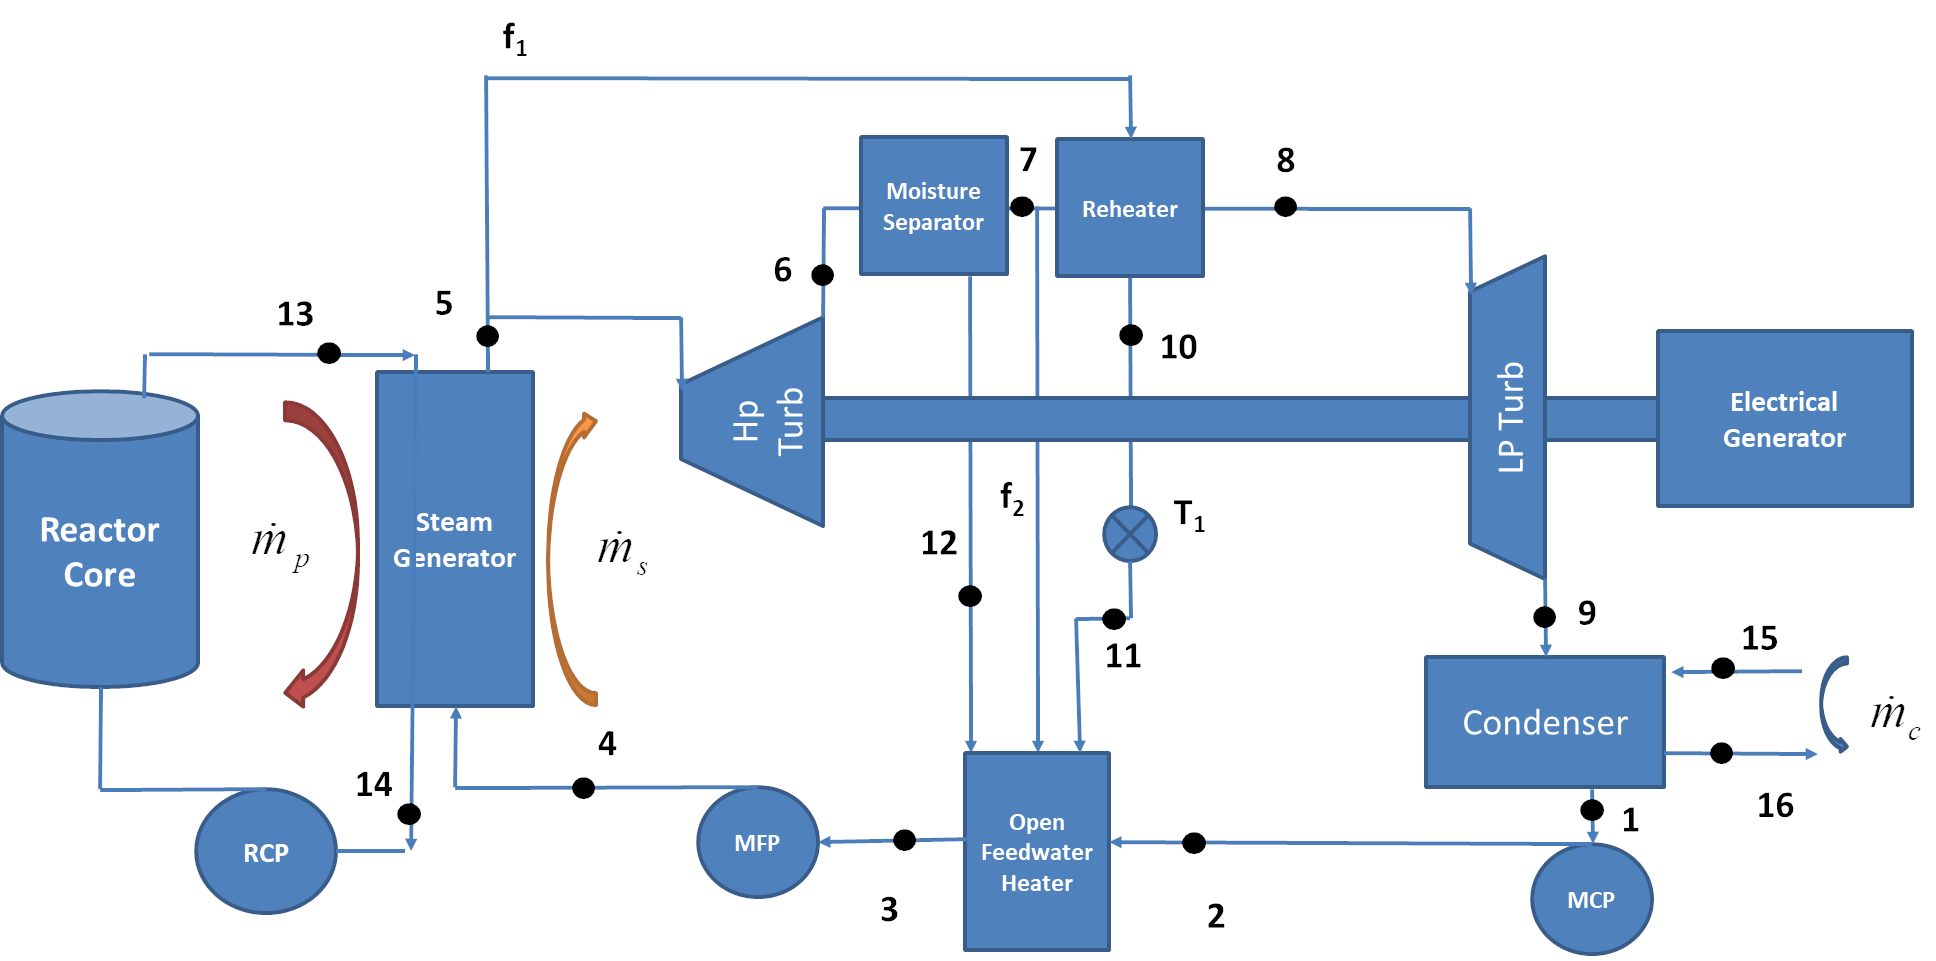
\includegraphics{Rankine_with_MS_and_OFWH_and_Reheat.png}
\caption[][0.75cm]{Rankine cycle with MS, OFWH and Reheat.}
\label{fig:RS_MS_OFWH_RH}
\end{figure}
 

The corresponding temperature-entropy sketch is provided in Figure \ref{fig:TS_MS_OFWH_RH}.  Note that the quality of the steam exiting the LP turbine at state point 9 has increased.
\begin{marginfigure}
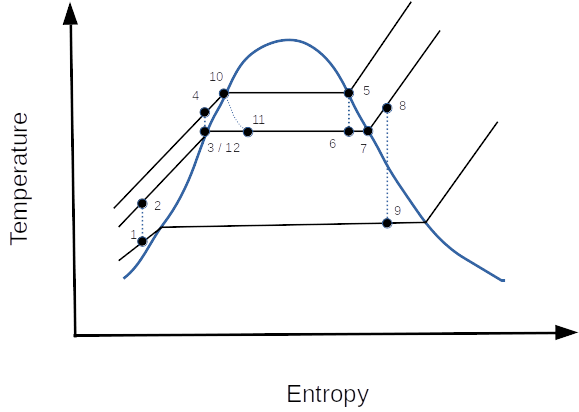
\includegraphics{TS_MS_OFWH_RH.png}
\caption{Temperature-entropy plot of modified cycle.}
\label{fig:TS_MS_OFWH_RH}
\end{marginfigure}
\newthought{There are a couple} of notable features of this cycle:
\begin{enumerate}
\item We use steam extracted upstream of the HP turbine\marginnote[0.25cm]{\textbf{Note:} Re-heat steam mass flow rate is typically around 5 percent of $\dot{m}_s$.} as the heat source to re-heat steam exiting the moisture separator. 
\item A new type of system component has been used between state points 10 and 11.  This device, which is referred to as a ``trap'' ($T_1$), allows for isenthalpic\marginnote{\textbf{Isenthalpic} means ``constant enthalpy.''} expansion of a working fluid; this is needed since the fluid at state point 10---which we will conventionally model to be in the saturated liquid state---is at higher pressure than the OFWH.  As a result of this expansion, the fluid at state point 11 will typically be a saturated mixture.
\end{enumerate}

\subsection{``First-Law'' Analysis of Modified System}
This cycle is more complicated than the last one.  We have two flow extractions ($f_1$ and $f_2$) that we need to solve for.  Consequently, we will need two equations to find a solution.  These equations will come from the energy balance for the open feedwater heater and the re-heater.  

\newthought{Using the conventions} for calculating flow fractions established in the last example, the energy balance for the OFWH is given as follows:\marginnote{\textbf{HEALTH WARNING: }you should take some time to study this equation; make sure every term makes sense and build confidence that you could derive this yourself.}
\begin{align*}
\Sigma \dot{E}_{\text{out}} &= \Sigma \dot{E}_{\text{in}} \\
\dot{m}_s h(3) &= \dot{m}_s [(1-f(1))(1-x(6))h(12) + (1-f(1))x(6)f(2)h(7)\dots \\
               & \ \ \ \ + f(1)h(11) + (1-f(1))(x(6))(1-f(2))h(2) ]
\end{align*}

The energy balance for the re-heater reads as follows:
\begin{align*}
\Sigma \dot{E}_{\text{out}} &= \Sigma \dot{E}_{\text{in}} \\
\dot{m}_s(1-f(1))x(6)(1-f(2))(h(8)-h(7))&=\dot{m}_s f(1)(h(5)-h(10))
\end{align*}

Both of these equations must be solved simultaneously to find $f(1)$ and $f(2)$.  These are both non-linear equations and, for general cycle analyses, can be quite difficult to find without computational help.  In the next lecture we will discuss MATLAB tools for carrying out the required calculations.




\chapter{Lecture 6 - Solving Multi-Variable Non-linear Equations in MATLAB}
\label{ch:ch6}
\section{Objectives}
The objectives of this lecture are:
\begin{itemize}
\item Describe the types of multi-variable non-linear equations that arise in analyzing complex thermodynamic cycles; and
\item Describe in detail how to use the built-in MATLAB function FMINCON
\end{itemize}

\section{Multi-variable Non-linear Equation}
In the last lecture, we analyzed a Rankine cycle with a moisture separator, re-heater, and an open feedwater heat exchanger.  In performing the analysis of the cycle, we arrived a two non-linear equations expressing conservation of energy for the re-heater and the open feedwater heater.  

For the OFWH:\marginnote{\textbf{Note: } For this example, assume that all state point property values and mass flow rates such as $h$, $x$, and $\dot{m}_s$ are known.

This will be the case for most cycles you analyze; you will be given enough information to find most/all state point properties but you will need to solve the non-linear equations to get the flow rates.}
\begin{multline}
\dot{m}_s h(3) = \dot{m}_s [(1-f(1))(1-x(6))h(12) + (1-f(1))x(6)f(2)h(7) + \dots \\
 f(1)h(11) + (1-f(1))(x(6))(1-f(2))h(2) ] 
\label{eq:Ebal_OFWH1}
\end{multline}

For the re-heater:
\begin{equation}
\dot{m}_s(1-f(1))x(6)(1-f(2))(h(8)-h(7)) = \dot{m}_s f(1)(h(5)-h(10))
\label{eq:Ebal_RH1}
\end{equation}

\newthought{These equations will be} presented in MATLAB format to facilitate the discussion.  As the equations are re-written in MATLAB form, we will also re-formulate the equations so they are amenable to solution with a tool like FMINCON.  Specifically, we will put all terms of the equation on one side.

\begin{minipage}{\linewidth} 
\begin{lstlisting}[caption=Energy balance equations in MATLAB format]
% f = [f1,f2]
OFWH_heatBalance = @(f) (1-f(1))*(1-f(2))*x(6)*(h2) + ...
f(1)*h(11) + (1-f(1))*x(6)*f(2)*h(7) + ...
(1-f(1))*(1-x(6))*h(12) - h(3);

ReHeater_heatBalance = @(f) f(1)*h(5) + ...
(1-f(1))*x(6)*(1-f(2))*h(7) - ...
( f(1)*h(10) + (1-f(1))*x(6)*(1-f(2))*h(8) );
\end{lstlisting}
\end{minipage}
Now we have two in-line functions that, given the correct values for $f_1$ and $f_2$, will be equal to zero.  We have re-cast our problem into a ``root-finding'' problem; one that many computational tools have been developed to solve.

\newthought{The way} we are going to solve this is using the built-in MATLAB function FMINCON.  FMINCON is a function for solving a constrained minimization problem for a non-linear function with multiple variables.  FMINCON expects only one equation to solve, so we will need to combine the 2 equations above into a single equation.  We will do this as follows:

\begin{lstlisting}[caption=Combine two heat balace equations into one.]
balance = @(f) abs(OFWH_heatBalance(f)) + ...
abs(ReHeater_heatBalance(f));
\end{lstlisting}
We want to find the values of $f(1)$ and $f(2)$ such that ``balance'' is minimized.  It should be clear that:
\begin{enumerate}
\item minimum possible value of ``balance'' is zero; and
\item ``balance = 0'' corresponds to satisfying both of the energy conservation equations for the OFWH and the RH.\sidenote[][-1.75cm]{This is only true because we use the absolute value function on each heat balance equation individually.  If we omitted the absolute value function then the minimization algorithm would drive the balance function towards negative infinity; if we used the absolute value function on the sum of the functions then positive errors for the OFWH could be offset by negative errors for the re-heater.}
\item We need to find this minimum value while constraining $f(1)$ and $f(2)$ to the interval $[0,1]$.\sidenote[][0.25cm]{Referencing the schematic from the previous lecture, $f(1)$ is the fraction of steam drawn off for re-heat and $f(2)$ is the fraction of steam flowing out of the moisture separator extracted and sent to the OFWH.  Since both are defined as flow fractions, they cannot be negative and they cannot be greater than 1, corresponding to 100 percent.}
\end{enumerate}

\newthought{The MATLAB function FMINCON} attempts to find a constrained minimum of a function of several variables. The function signature is:

\begin{lstlisting}
X = fmincon(FUN,X0,A,B,Aeq,Beq,LB,UB,NONLCON,OPTIONS);
\end{lstlisting}

The arguments for FMINCON are as follows:
\begin{itemize}
\item FUN: this is the function that you hope to minimize; as illustrated here, this is the function ``balance.''
\item X0: this is a vector providing the initial guess for each variable in the function.  For this example X0 must have two entries, one for the initial guess for $f(1)$ and $f(2)$.  A reasonable value for X0 in this case would be: [0.5 0.5]
\item A and B.  These arguments allow the user to express linear inequality constraints between the non-linear variables.  The inequalities are expressed as: $AX \le B$ so if, for example, we want to enforce an inequality such as $f(1) > f(2)$, this could be written mathematically as $-f(1)+f(2) \le 0$; we would set A = [-1,1]; and B = [0].  For the example we are using for this lecture, no such inequality constraint exists so we would set A = [] and B = [].  
\item Aeq and Beq.  This is the same as above but are equality constraints instead of inequality constraints.  If, for example, we want to enforce the constraint that $f(1) + f(2) = 1$, we would set A = [1,1] and B = [1]. For this problem we have no such constraints so we should set Aeq = [] and Beq = [].

\item LB and UB: these arguments are where you provide the lower bound and upper bound for each of your variables.  For multi-variable problems, these should be entered as vectors.

\item NLCON: this argument allows for you to provide non-linear constraints between the dependent variables.  We will not be using this functionality and set this argument to NLCON = [].
\item OPTIONS.  This argument allows you to provide keyword-value pairs for various options.  The argument must have a specific form and is most easily set using another built-in function ``optimoptions''.  Use of this feature will be illustrated in the next code listing.
\end{itemize}

Using this information, we can provide values for the function arguments and find the constrained minimum for our equations as follows:

\begin{lstlisting}[caption=Set arguments and call FMINCON to find constrained minimum]
x0 = [0.5 0.5]; % a reasonable guess within the lower and upper bounds of the variables
A = [];  % no linear inequality constraints
B = [];
Aeq = []; % no linear equality constraints
Beq = [];
lb = [0 0];
ub = [1 1];
nlcon = []; % no nonlinear constraints
options = optimoptions('fmincon','Display','none'); % suppress extensive output
% other commonly used option sets:
% options = optimoptions('fmincon','Display','iter');
% options = optimoptions('fmincon','Algorithm','sqp');
% select constrained minimization algorithm.  Default is 'interior-point'
% other options: 'sqp','sqp-legacy','active'set',
% and 'trust-region-reflective'.  See documentation.
%

[f,fval,exitflag] = fmincon(balance,x0,A,B,Aeq,Beq,lb,ub,nlcon,options);

% report the results
fprintf('Flow fraction for reheat steam = %5.4f \n',f(1));
fprintf('Flow fraction to OFWH from M/S exit = %5.4f \n',f(2));
\end{lstlisting}

  


\chapter{Lecture 7 - Rankine Cycle with Closed Feedwater Heaters}
\label{ch:ch7}
\section{Objectives}
The objectives of this lecture are:
\begin{itemize}
\item Describe Closed Feedwater Heaters (CFWH)
\item Discuss the ``Cascade Back'' and ``Pump Forward'' arrangements for dealing with CFWH drains.
\item Provide some design and modeling notes.
\end{itemize}

\section{Closed Feedwater Heaters}
\newthought{In a previous lecture} we learned about open feedwater heaters (OFWH).  OFWHs are used in the Rankine Cycle to pre-heat feedwater before entering the Steam Generator.  In workshop exercises you could see how use of OFWHs reduce overall exergy destruction (irreversibility) and improve cycle thermal efficiency.  

Closed feedwater heaters (CFWHs) perform the same role.  The differences is that in CFWHs the fluids do \underline{not} mix.  A simple schematic is given in Figure \ref{fig:CFWH_1}.
\begin{marginfigure}
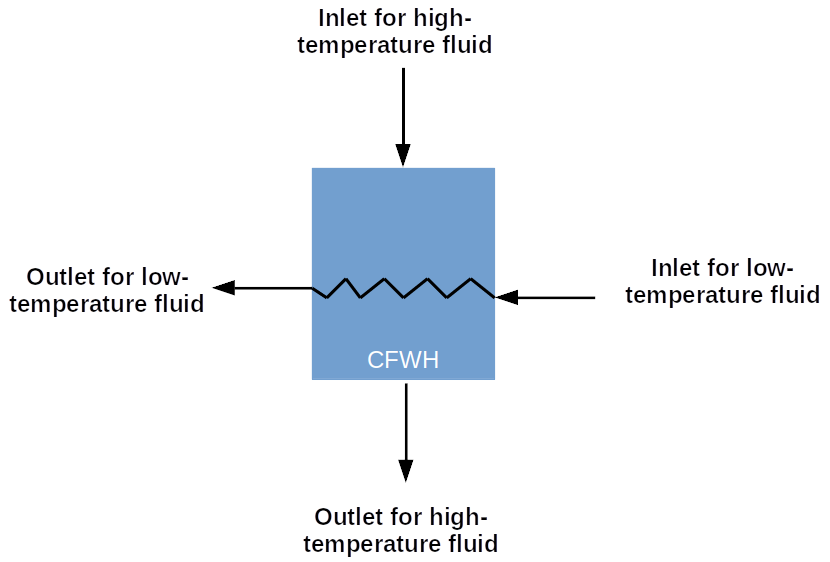
\includegraphics{CFWH_simple_schematic.png}
\caption{Simple CFWH schematic.}
\label{fig:CFWH_1}
\end{marginfigure}
\newthought{The high-temperature fluid} is normally steam, extracted from a selected turbine stage, and the low-temperature fluid being heated is normally feedwater.  The low-temperature water is, for all of our applications, a subcooled liquid.  The high-temperature fluid is, for most nuclear applications, a saturated mixture of relatively high quality ($x \ge 80$ percent) although in principle it could be superheated.  The outlet for high temperature fluid is normally a saturated or slightly subcooled liquid. For CFWHs the outlet of the low temperature fluid is usually still a subcooled liquid albeit at a higher temperature than it was at the inlet. 

Although it is beyond the scope of this class, it is worthwhile to consider the added complexity of modeling---and at some point in our career designing---a heat exchanger where one of the fluids undergoes phase changes.  A somewhat more realistic schematic representation of a CFWH is showing in Figure \ref{fig:CFWH_2}.  Here, in the case that the extraction steam is above saturation temperature, the steam is reduced to saturation temperature in the ``de-superheater'' region on the heat exchanger.  Heat transfer correlations used for single-phase convective heat transfer from the steam to the heat exchanger tubes would be used to model heat exchanger performance.  In the ``condenser'' region, the complicated phase change process occurs where steam is converted to saturated liquid.  In the ``condensate cooler'' region, once again single-phase heat transfer prevails as the liquid water gives up its energy to the incoming feed flow.

\begin{marginfigure}
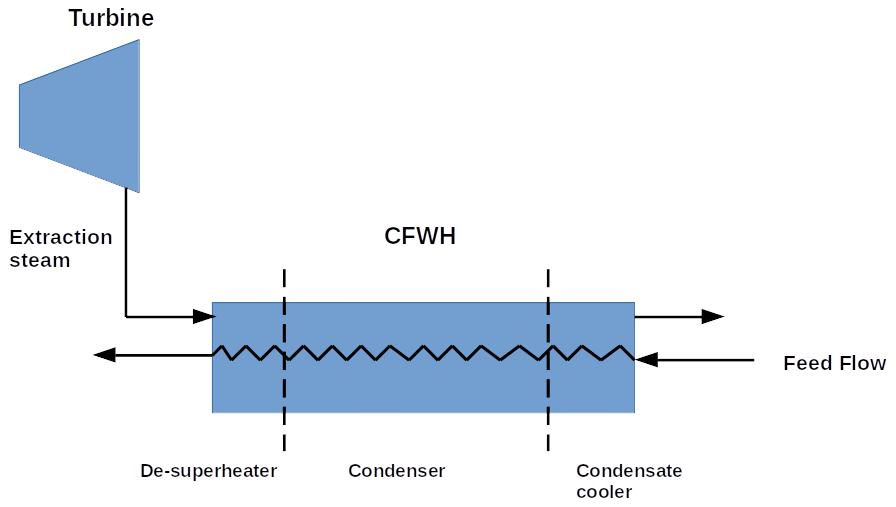
\includegraphics{CFWH_schematic.png}
\caption{Conceptual schematic of a CFWH.}
\label{fig:CFWH_2}
\end{marginfigure}


\newthought{Once the heating fluid} exits the CFWH, it has to go somewhere.  In OFWHs, the heating fluid was simply carried away with the (now preheated) feedwater.  In a CFWH, the high-temperature fluid exit needs to be directed somewhere else to be integrated into the feed-flow stream.  There are two conventional choices for doing this:
\begin{enumerate}
\item ``Drain Cascade Back''---type 1
\item ``Drain Pump Forward''---type 2
\end{enumerate}

The Rankine cycle schematic shown in Figure \ref{fig:RC_MS_RH_OFWH_CFWH_t1} illustrates a type 1 arrangement.
\begin{figure}
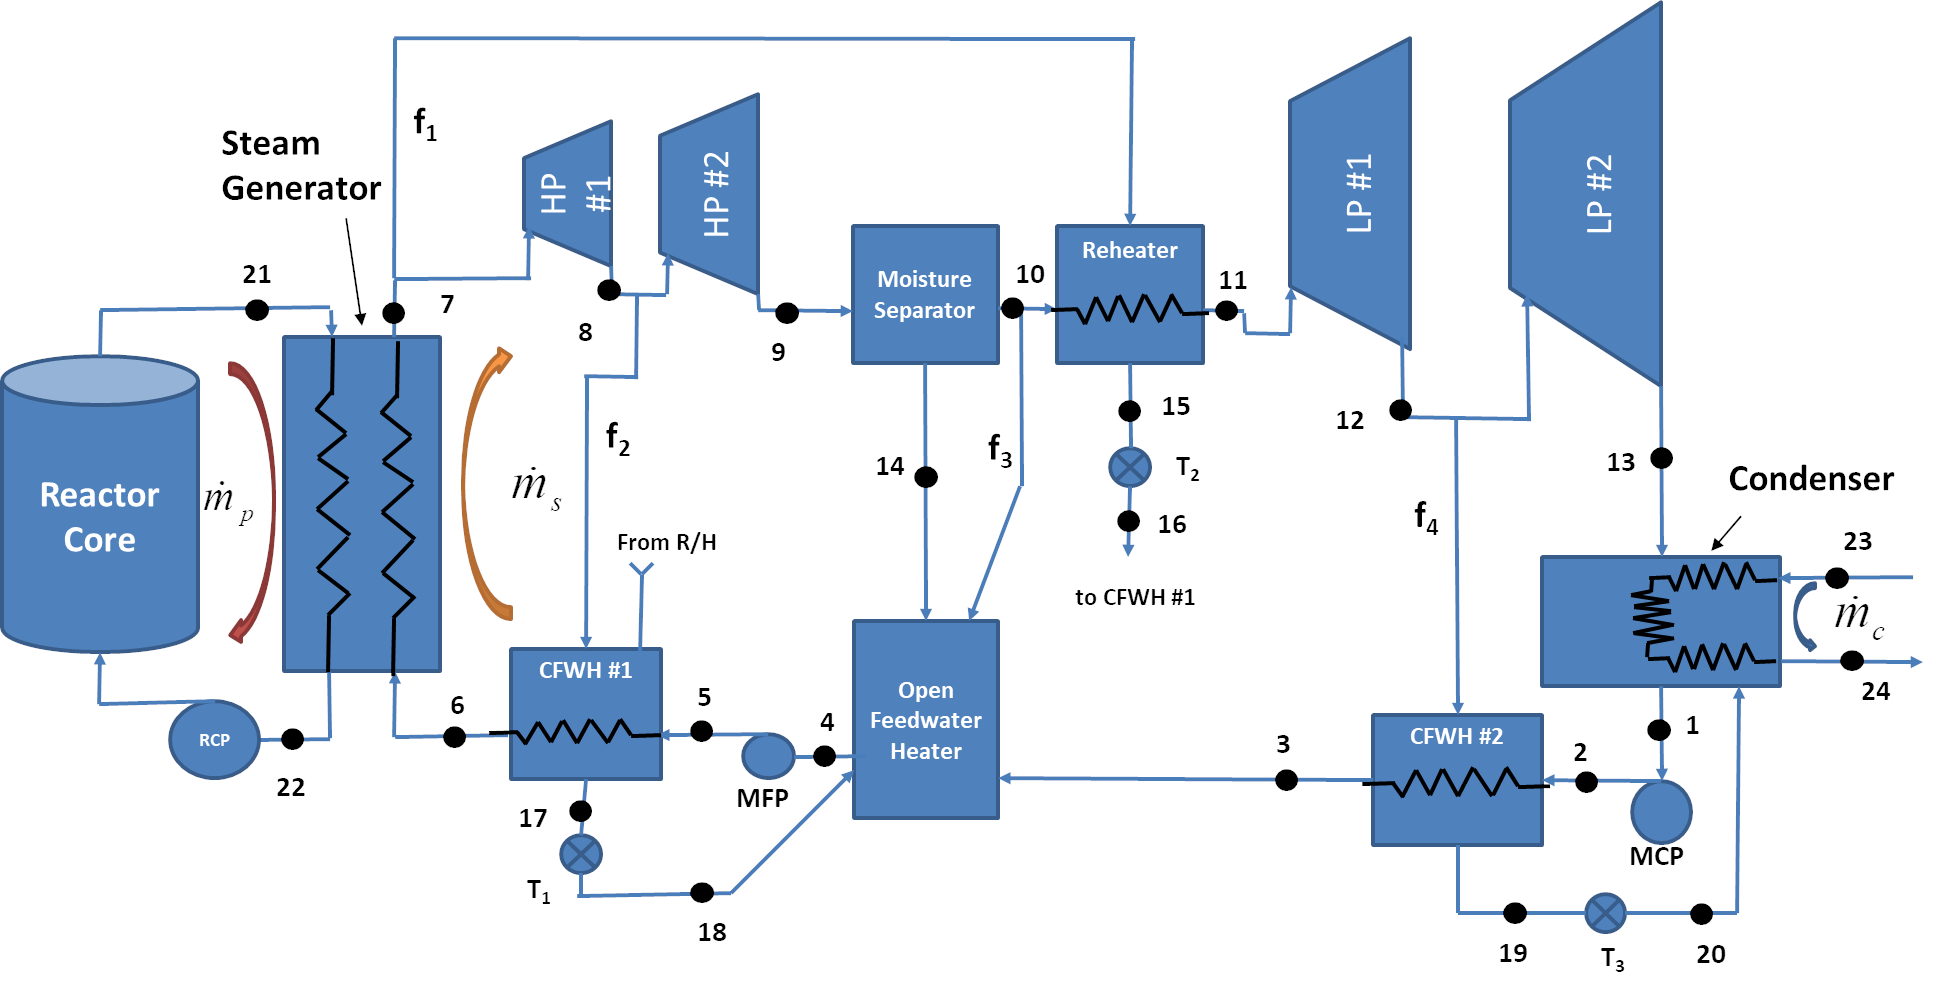
\includegraphics{Rankine_with_MS_RH_OFWH_CFWH_type1.png}
\caption{Complex Rankine cycle with type 1 ``Drain Cascade Back'' CFWH arrangement.}
\label{fig:RC_MS_RH_OFWH_CFWH_t1}
\end{figure}
CFWH \#1 has two high-temperature fluid inputs: one is extraction steam from the turbine labeled ``HP \#1''; the other comes from the re-heater exit.\marginnote[-0.5cm]{\textbf{Question: }Why is it probably better to direct the fluid at state point 16 to CFWH \#1 rather than to the OFWH, CFWH \#2, or the Condenser?}  The heating fluid in the CFWH all exits through a common drain.  This drain is directed to the OFWH.  Since all fluids entering the OFWH must be at the same pressure, this fluid is expanded through a trap (labeled $T_1$) entering the OFWH at state point 18.

\newthought{A cycle with multiple} CFWHs will normally cascade the heat exchanger drains in order to extract maximum reheating benefit from the extraction steam.  A simplified schematic of Rankine cycle employed with the Experimental Breeder Reactor II is presented in Figure \ref{fig:EBRII}.\cite{koch2008experimental}
\begin{figure}
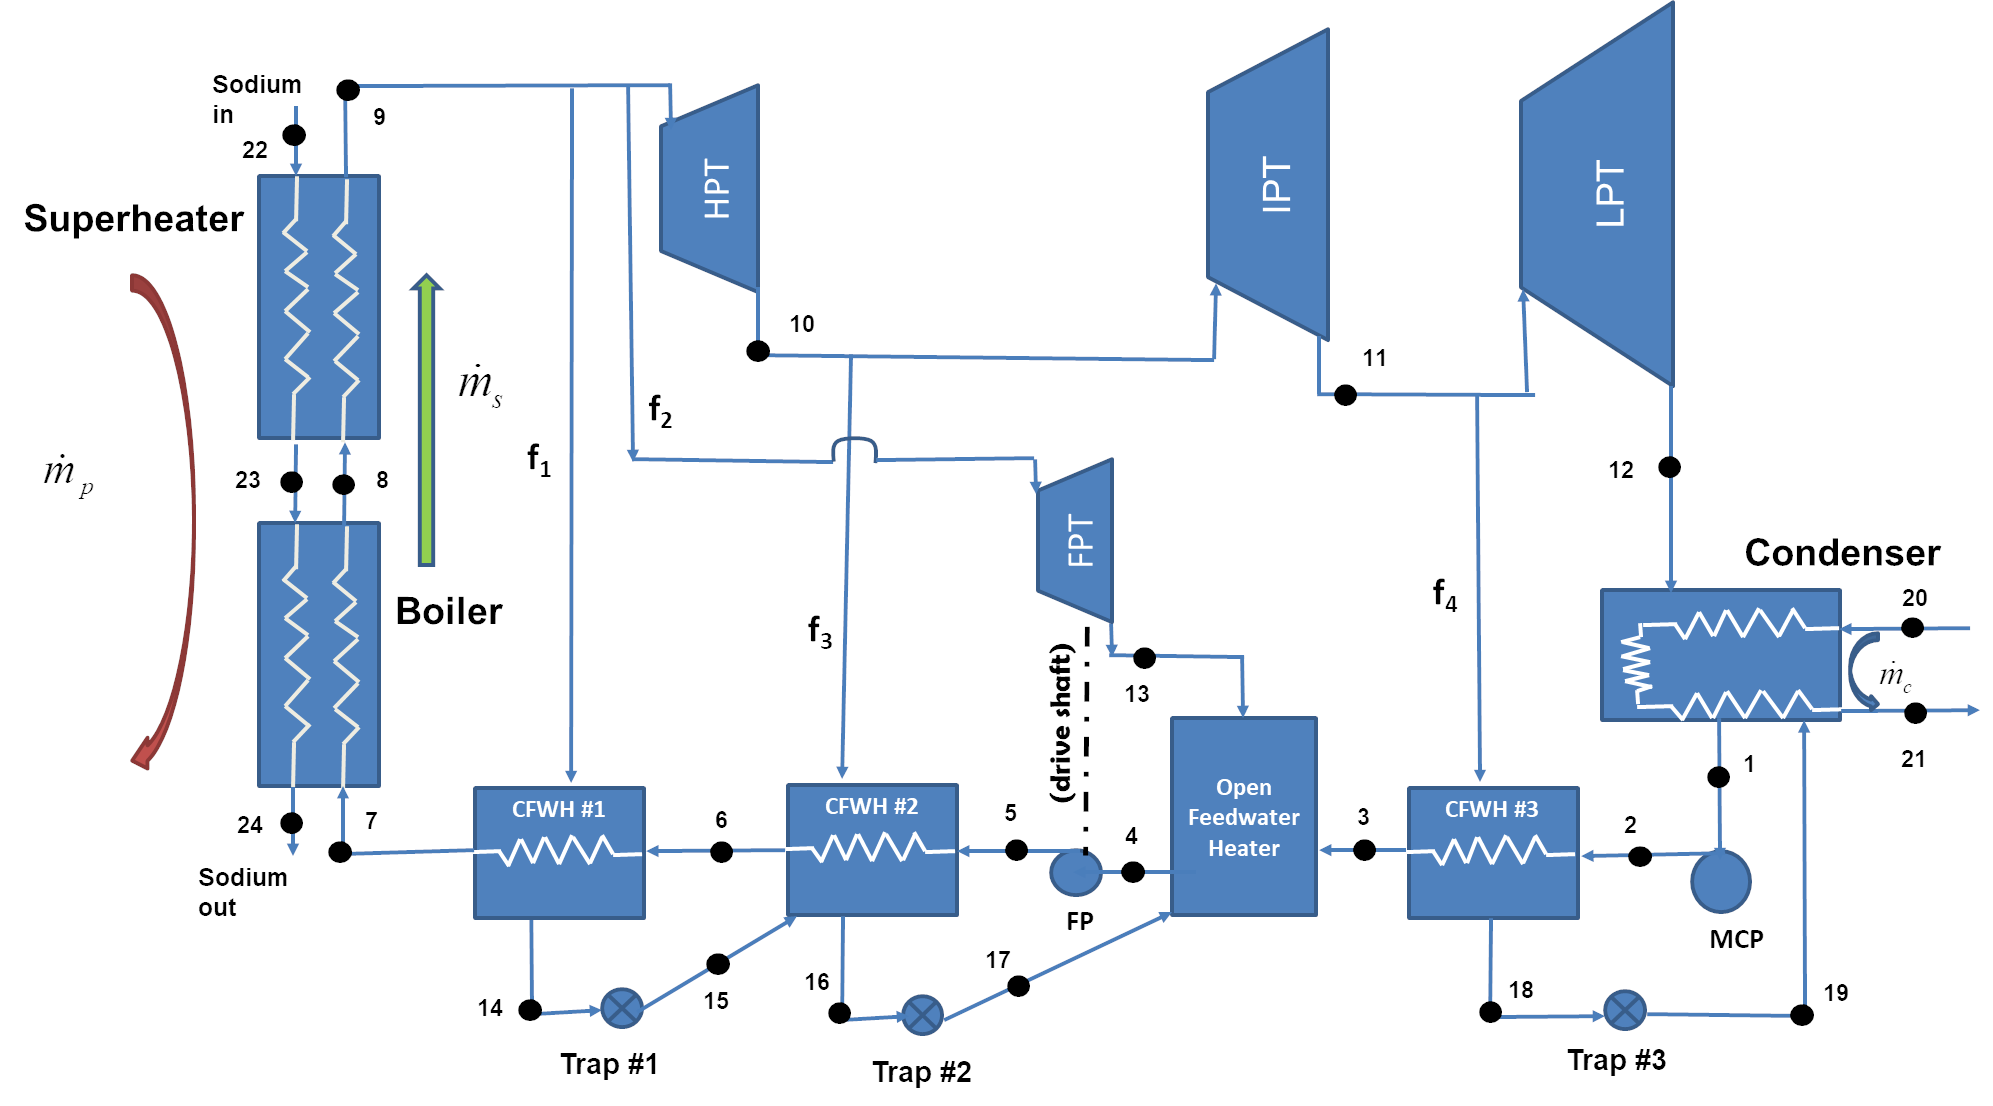
\includegraphics{EBR_II.png}
\caption[][1cm]{Simplified schematic of the Experimental Breeder Reactor II energy conversion cycle with cascaded CFWH drains.}
\label{fig:EBRII}
\end{figure}


\newthought{A type 2 arrangement} for a CFWH is illustrated in Figure \ref{fig:CFWH_type2}.  Notice the extra state point required at the exit of the CFWH after the point where the drain pump discharge is mixed in to the feedwater flow.  
\begin{marginfigure}
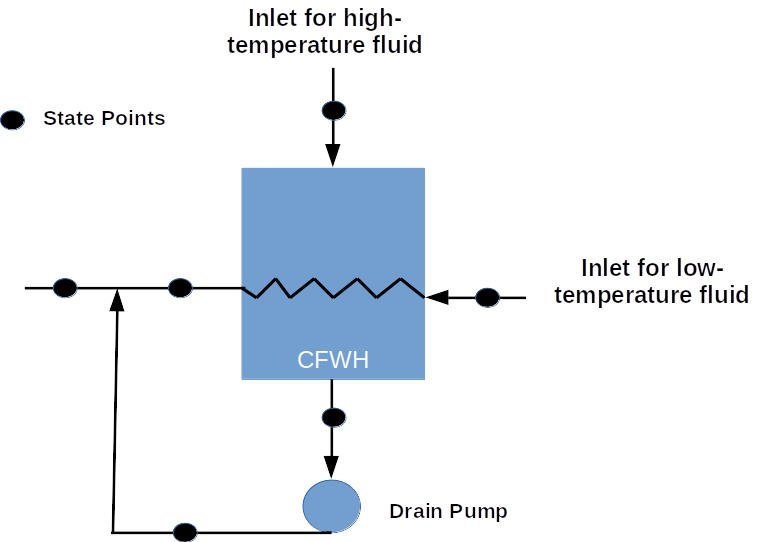
\includegraphics{Pump_Forward_CFWH_Drain.png}
\caption{Schematic of CFWH with type 2 drain pump arrangement.}
\label{fig:CFWH_type2}
\end{marginfigure}




\section{Design and Modeling Notes}
There are too many details on the variations of Rankine cycle designs in order to hope to cover them all in one course, much less one lecture.  Here I provide a set of bullet-points to try and summarize some general principles that one can get by examining modern and relevant Rankine cycles for nuclear energy conversion:

\begin{itemize}
\item Rankine cycles typically utilize a mixture of OFWHs and CFWHs (e.g. 5-6 CFWHs + 1 or 2 OFWHs).  
\item BWRs generally will not use OFWHs due to the need to contain gaseous radionuclides in the coolant.\sidenote{OFWHs usually include a dearator function where air and other non-condensable gasses are vented from the feedwater and ejected to the atmosphere. In a BWR some of those gasses may be radioactive.}  
\item High pressure / low temperature outlet from the CFWH is usually modeled as having the same (or nearly the same) temperature as the incoming heating steam.  
\item High temperature / low pressure outlet from CFWH is usually modeled as a saturated liquid (or slightly sub-cooled).
\item Extraction steam pressures are often chosen such that the steam temperature (in each extraction stream) is reduced in roughly equal increments.
\item ``Drain Pumped Forward'' CFWHs result in slightly higher thermal efficiency but:
\begin{enumerate}
\item Requires another pump (that might break); and
\item Combinations of drain-forward and drain cascade back possible (of course).
\end{enumerate}
\item How much is it worth to increase thermal efficiency a little bit by adding all of this complexity:
\begin{itemize}
\item For a navy nuclear powered warship?
\item for a commercial nuclear power plant operator?
\end{itemize}
\end{itemize} 


\chapter{Assignment \#3: Rankine Cycle, Enhanced Regeneration}
\label{ch:ass3}

\begin{fullwidth}
\newthought{Consider the } Rankine cycle depicted in the figure below:

\begin{figure}
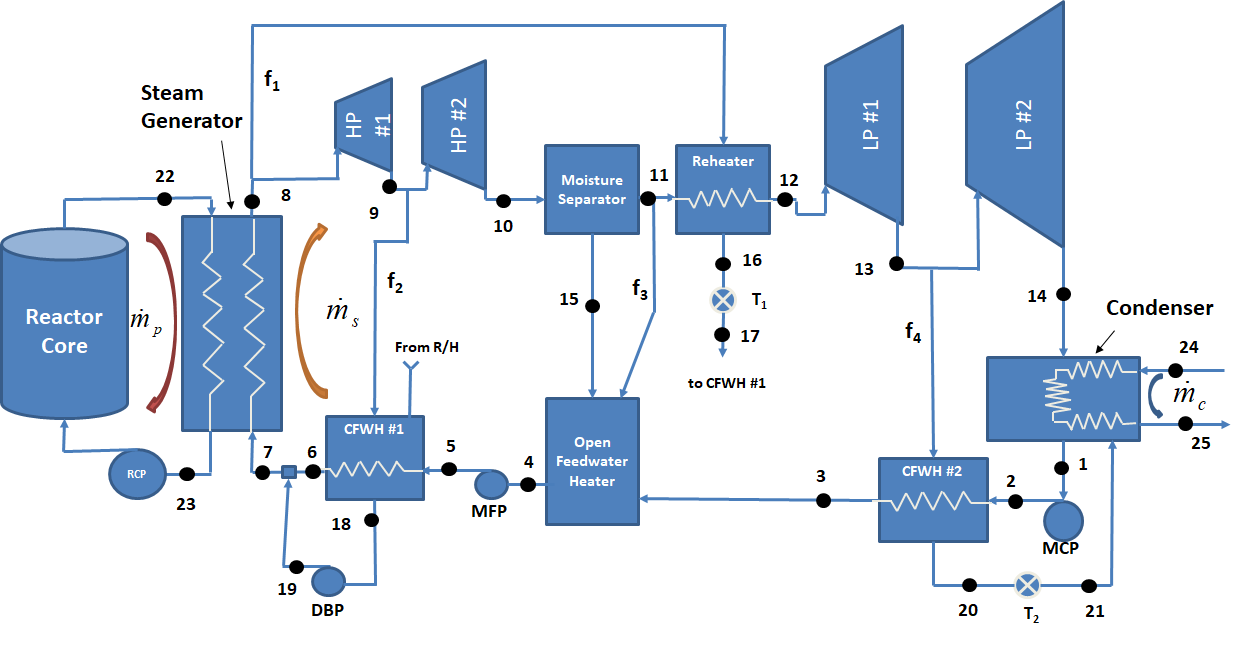
\includegraphics[width=12.0cm]{PowerCycleSchematic.png}
\caption{Power Cycle for Assignment \#3.}
\end{figure}

\begin{table}
\begin{tabular}{c | l || c | l}
\toprule
State Point & Notes & State Point & Notes \\
\hline
1 & P = 1.5 psia, x = 0.0 & 2 & P=164 psia \\
\hline
3 & T=T$_{\text{sat@ 62 psia}}$, P=164 psia & 4 & P = 164 psia\\
\hline
5 & P=838 psia, $\eta_{\text{MFP}} = 0.88$ & 6 & P = 838 psia, T=T$_{\text{sat @ 410 psia}}$ \\
\hline
7 & P = 838 psia & 8 & P=838 psia, x=1.0 \\
\hline
9 & P = 410 psia & 10 & P=164 psia \\
\hline
11 & P=164 psia & 12 & P=164 psia, T=490$^{\circ}$F \\
\hline
13 & P=62 psia & 14 & P=1.5 psia \\
\hline
15 & P=164 psia & 16 & P=838 psia, x=0.0 \\
\hline
17 & P=410 psia, isenthalpic expansion through T$_{1}$ & 18 & P=410 psia, x=0.0 \\
\hline
19 & P=838 psia & 20 & P=62 psia, x=0.0 \\
\hline
21 & P=1.5 psia, isenthalpic expansion through T$_{2}$ & 22 & P=2240 psia, T=610$^{\circ}F$ \\
\hline
23 & P=2240 psia, T=535$^{\circ}$F & 24 & P=14.7 psia, T=91$^{\circ}$F \\
\hline
25 & P=14.7 psia, T=115$^{\circ}$F & & \\
\hline
$\dot{m}_{p}$ & $113.5 \times 10^{6}$ lb$_{\text{m}}$/hr & Dead State & T$_{o}$=551$^{\circ}$R, P$_{o}$=14.7 psia \\
\bottomrule
\end{tabular}
\end{table}

\section{First Law Analysis}
\begin{enumerate}
\item Calculate pressure, temperature, enthalpy, entropy, quality, and specific flow exergy for each state point. [use USCS units throughout]

\vspace{1.0 cm}

\item Form energy-balance equations for CFWH\#1 and CFWH\#2.  Use \emph{fmincon} to solve for the flow fraction components of $f_1$, $f_2$, $f_3$, $f_4$, and the enthalpy at state point 7. [ flow fractions are unitless, $h_7$ is in BTU/lb$_m$]

\vspace{1.0cm}

\item Find the specific work for all pumps and turbines.[BTU/lb$_m$]

\vspace{1.0 cm}
\item Find the specific heat added in the SG and specific heat rejected in the condenser. [BTU/lb$_m$]

\vspace{1.0 cm}

\item Calculate the mass flow rate of steam from the steam generator $(\dot{m_{s}})$ and mass flow rate of condenser cooling water $(\dot{m_{c}})$.
\vspace{1.0cm}

\item Verify that $w_{\text{net}} = q_{\text{net}}$.

\vspace{1.0 cm}

\item What is the thermal efficiency for this cycle?

\end{enumerate}

\section{Second Law Analysis}

\begin{enumerate}[resume]
\item Calculate the total exergy transfer by work for the cycle. [BTU/hr]

\vspace{1.0cm}
\item Calculate the rate of exergy destruction in each component of the cycle. [BTU/hr]

\vspace{1.0cm}

\item Verify that the second law energy balance is satisfied:
$$\text{Exergy in - Exergy out = Exergy Destroyed + Exergy Transfer Through Work}$$

\vspace{1.0cm}

\item \textbf{\emph{Question for discussion:}} What components of the NSSS are most responsible for exergy destruction?  What design modifications would you consider to improve thermal efficiency?
\end{enumerate}

\end{fullwidth}

\chapter{Lecture 8 - Boiling Water Reactors and Supercritical Water Nuclear Reactors}
\label{ch:ch8}
\section{Objectives}
The objectives of this lecture are:
\begin{itemize}
\item Qualitative comparison between BWR and SCWR technologies
\item Quantitative example of SCWR energy conversion cycle
\item Practice analysis of complex Rankine cycles
\end{itemize}

\index{boiling water reactor}
\section{BWRs and Direct Cycles}
Early BWRs were built with the hopes of simplifying the system by having a direct steam cycle.  A schematic is shown in Figure \ref{fig:simple_BWR}.  
\begin{marginfigure}
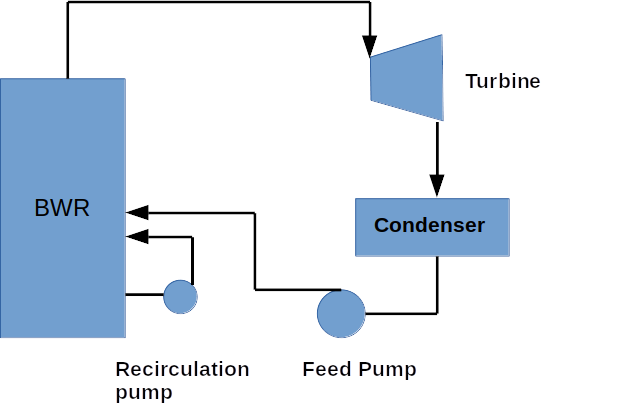
\includegraphics{simple_BWR.png}
\caption{Simplified BWR schematic.}
\label{fig:simple_BWR}
\end{marginfigure}
\newthought{Apart from the need} to contain radioactivity in the working fluid, this cycle is not, in principle, much different than the Rankine energy conversion cycle associated with a PWR.  Some of the advantages of a ``more simple'' direct cycle are mitigated by the lower power density achievable in the core of a BWR.\marginnote{\textbf{Note: }Typical core average power density for a BWR is 50 kW/l; roughly one half that achievable with a PWR.}  Most notably, the overall system for a given power output, is roughly as large as a PWR resulting in comparable construction costs; thus BWRs share one of the most significant problems with PWRs: high capital costs.

\section{Supercritical Water Nuclear Reactor}
\index{supercritical water reactor}
\newthought{One Gen IV concept} that has been developed with the aim of addressing the power-density issue with direct-cycle light water reactors is the Supercritical Water Nuclear reactor.\cite{tsiklauri2005supercritical} For this cycle, the water is maintained above the critical pressure throughout the heat-addition phase.  Good heat transfer can still be achieved without phase change and the prevention of bulk boiling prevents hydraulic instabilities that can be associated with BWR cores.  

\newthought{Additional notes are} provided in bullet-format:
\begin{itemize}
\item Elimination of phase change in the core eliminates the need for complex moisture separation equipment for fluid exiting the reactor core.  
\item Lack of phase change in the core also shifts the power distribution higher in the core relative to a typical BWR; the combination of this effect along with elimination of the moisture separation equipment favors locating the control rods at the top of the core.
\item Overall result is a smaller reactor pressure vessel and reduced containment size.
\end{itemize}
A schematic comparison of the size of a SCWR relative to competing PWR and BWR technologies is presented in Figure \ref{fig:SCWR_size}.
\begin{figure}
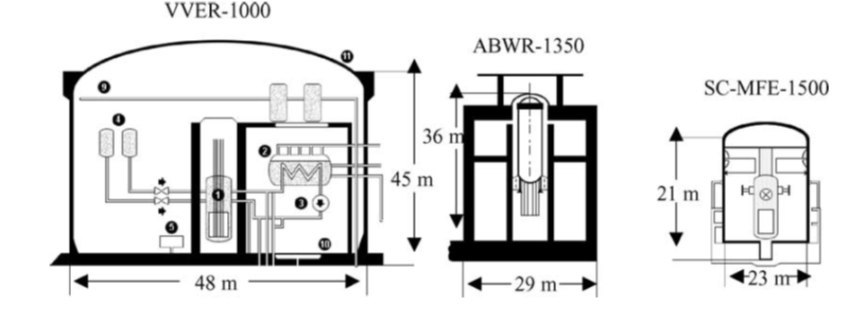
\includegraphics{BWR_SCWR_size_comparison.png}
\caption{Comparison of the size of containments for SC-MFE-1500, ABWR-1350 and VVER-1000.}
\label{fig:SCWR_size}
\end{figure}

\newthought{Even though moisture separation} equipment is not needed in the pressure vessel, there is a need for moisture separation equipment in the energy conversion cycle.  A temperature-entropy plot is drawn to scale in Figure \ref{fig:SCWR_TS}.  Even with very high core outlet temperature, when the supercritical fluid is expanded to low pressure moisture content of the working fluid becomes unacceptably high. Typical coal-fired steam plants operating at supercritical pressures deal with this issue by using one or more stages of reheat.  For nuclear powered systems, the steam piping arrangement necessary to use nuclear power for reheat can be impractical. For this cycle we will use additional moisture separation stages. 
\begin{marginfigure}
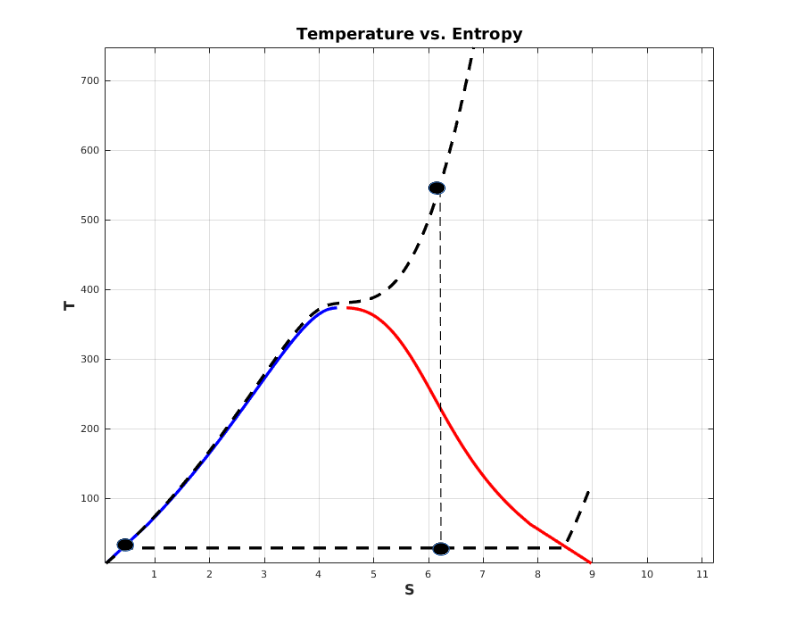
\includegraphics{SCWR_TS.png}
\caption{Temperature-entropy plot for SCWR drawn to scale.}
\label{fig:SCWR_TS}
\end{marginfigure}
A schematic of a potential SCWR energy conversion cycle is shown in Figure \ref{fig:SCWR_cycle}. Analysis of this cycle involves some complexity insofar as the flow fractions for each branch of the cycle needs to be determined but the details of such calculations are straight-forward.  Significant plant parameters are listed in Table \ref{tab:SCWR_params}.  Note the high thermal efficiency and high net specific work; with the moisture separators in use, the minimum turbine exhaust quality is more than 85 percent.  

\begin{margintable}
\begin{tabular}{cc}
\toprule
Parameter & Value \\
\midrule
$T_9$, $P_9$ & 550$^{\circ}$C, 24 MPa \\
HP Turbine Outlet Pressures & 8.9, 6, and 1 MPa \\
LP Turbine Outlet Pressures & 200 kPa, 4 kPa \\
$\eta_T$, $\eta_P$ & 0.9 and 0.88 \\
$w_{\text{net}}$ & 948 kJ/kg \\
Thermal Efficiency & 47.3 percent \\
\bottomrule
\end{tabular}
\caption{SCWR Parameters.}
\label{tab:SCWR_params}
\end{margintable}
\begin{figure}
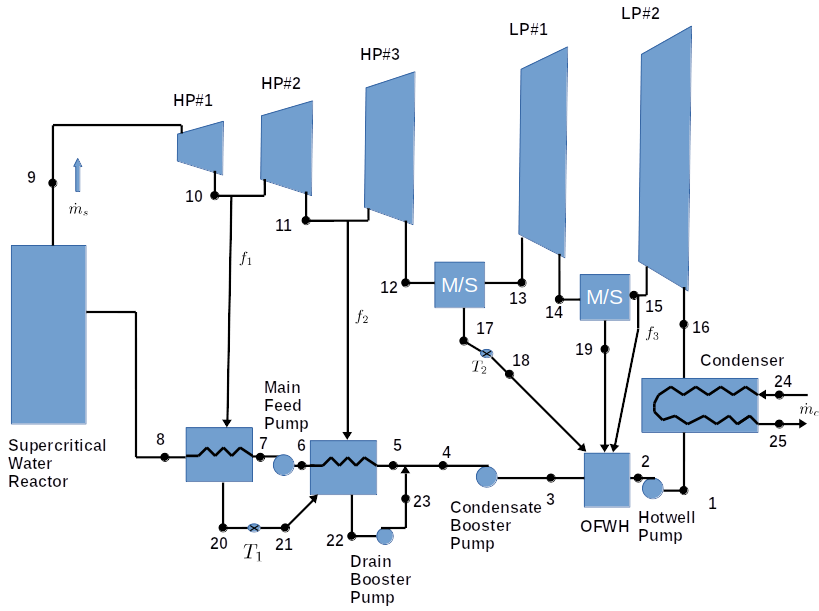
\includegraphics{SCWR_cycle.png}
\caption[][3cm]{SCWR power cycle with moisture separators. MATLAB code for a first-law analysis of this cycle is provided in the appendices.}
\label{fig:SCWR_cycle}
\end{figure}

\begin{example}
\textbf{Example calculations:} 
\begin{enumerate}
\item Write an expression for the specific work of Low Pressure Turbine \#2:

\emph{Answer:} $(h_{15}-h_{16})\left[(1-f_1)(1-f_2)x_{12}x_{14}(1-f_3) \right]$


\item Write an expression for the specific work of the Drain Booster Pump:

\emph{Answer:} $(h_{22}-h_{23})\left[f_1 + (1-f_1)f_2\right]$

\item Write an expression for the specific work of the Condensate Booster Pump:

\emph{Answer:} $(h_3 - h_4)[1 - (f_1 + (1-f_1)f_2)]$

\item Write an expression for the energy balance at the mixing point between the Condensate Booster Pump and CFWH \#2:

\emph{Answer:} $h_5 = [f_1+(1-f_1)f_2]h_{23} + [1-(f_1+(1-f_1)f_2]h_4$


\end{enumerate}
\end{example}



\begin{comment}
\begin{example}
\textbf{Challenge Problem:} Write an expression for the energy balance of the OFWH:
\emph{Answer:} 
\begin{multline*}
[1 - (f_1 + (1-f_1)f_2]h_3 = \\
(1-f_1)(1-f_2)x_{12}x_{14}(1-f_3)h_2 + \\
(1-f_1)(1-f_2)x_{12}x_{14}f_3h_{15} + \\
(1-f_1)(1-f_2)x_{12}(1-x_{14})h_{19} + \\
(1-f_1)(1-f_2)(1-x{12})h_{18} \\
\end{multline*}
\end{example}
\end{comment}



\chapter{Lecture 9 - Pinch-Point Temperature Difference}
\label{ch:ch9}
\section{Objectives}
The objectives of this lecture are:
\begin{itemize}
\item Describe pinch-point temperature difference ($\Delta T_{p}$) and show how to calculate it.
\item Show relationship between $\Delta T_{p}$ and exergy destruction rate in the Steam Generator (SG).
\item Compute $\Delta T_{p}$ for a few modern commercial PWRs.
\item Provide thumb rules/guidance for concept design use.
\end{itemize}

\index{Pinch-Point Temperature Difference}

\section{Description of $\Delta T_{p}$}
\newthought{The pinch-point temperature difference} is the minimum difference between the primary coolant and the secondary coolant in a PWR.  This is shown schematically in the temperature-entropy diagram in Figure \ref{fig:ppdp_TS}. An alternative representation of the process is shown in Figure \ref{fig:ppdp_hx}.
\begin{marginfigure}
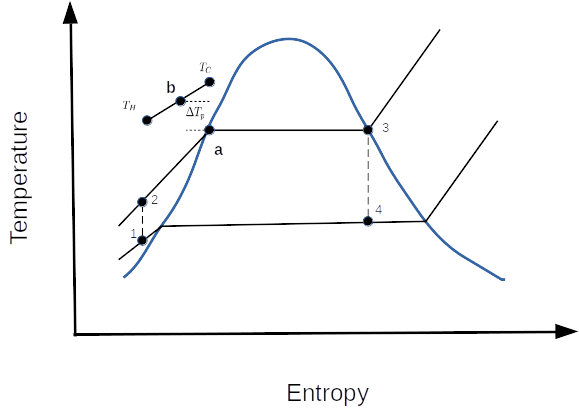
\includegraphics{pinch_point_TS.png}
\caption{Schematic illustration of $\Delta T_{p}$.}
\label{fig:ppdp_TS}
\end{marginfigure}


\begin{marginfigure}
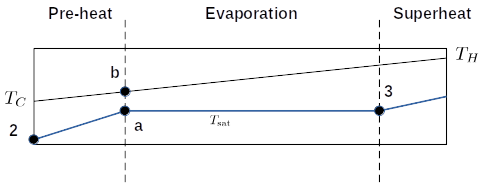
\includegraphics{pinch_point_hx.png}
\caption{Illustration of $\Delta T_{p}$.}
\label{fig:ppdp_hx}
\end{marginfigure}

\newthought{Let us take a moment} to discuss these representations:

\begin{itemize}
\item These representations are not intended to be taken literally.  The SG for most PWRs is, of course, not a once-through counter-flow heat exchanger as Figure \ref{fig:ppdp_hx} indicates.\sidenote{Although in fairness when the concept of $\Delta T_{p}$ was formulated, such SGs were in use and it probably seemed less crazy.} 
\item Consequently, one shouldn't expect to be able to point to the spot on a SG where $\Delta T_{p}$ is realized.
\item Nonetheless, $\Delta T_{p}$ can still be used as a useful engineering parameter because it relates to the relative temperature of the primary coolant and the steam generator. 
\end{itemize}

\newthought{In Heat Transfer class} you will learn one method for analyzing heat exchangers, like the SG, using the log-mean temperature difference. Equation \ref{eq:hx_eq} says that:
\begin{itemize}
\item The rate of heat transfer $(\dot{Q}_{\text{SG}})$ is equal to the product of the overall-heat transfer coefficient $(U)$\marginnote[-1.0cm]{\textbf{Note: }The overall heat transfer coefficient combines the effects conductive heat transfer through heat exchanger surfaces as well as convective heat transfer to/from the heated/cooled fluids.}, the heat transfer surface area $(A)$ and the log-mean temperature difference $(\Delta T_{\text{LM}})$\marginnote[0.25cm]{\textbf{Note: }Log-mean temperature difference is computed based on the difference in temperatures at the heat exchanger inlets and outlets. Specifically, $\Delta T_{\text{LM}} = \frac{\Delta T_{\text{side-a}} - \Delta T_{\text{side-b}}}{\ln{\frac{\Delta T_{\text{side-a}}}{\Delta T_{\text{side-b}}}}}$. Referencing Figure \ref{fig:ppdp_hx}, the log mean temperature difference is calculated as: $\Delta T_{\text{LM}} = \frac{(T_{H}-T_3) - (T_{C} - T_2)}{\ln{\frac{T_{H} - T_3}{T_C - T_2}}}$}; and
\item That heat transfer rate is also equal to the rate of heat transfer into the secondary system water and heat transfer from the primary coolant.
\end{itemize}

\begin{equation}
\dot{Q}_{\text{SG}} = UA\Delta T_{\text{LM}} = \dot{m}_s(h_3 - h_2) = \dot{m}_p(h_{H} - h_{C})
\label{eq:hx_eq}
\end{equation}


\newthought{This is the first time} so far in this course where we have attempted to relate the performance of a heat exchanger to any real-world parameters of the heat exchanger.  In past lectures, heat exchangers like feedwater heaters, SGs, and condensers were represented only as rectangles on a schematic with in-flows and out-flows and some expectation as to what the temperatures of the respective fluids would be.  No consideration was given as to what a heat exchanger would look like; how big it would be, what materials it would be made of, and if the expected performance was in any way realistic.

\newthought{To the extent} that this shortcoming is addressed at all, we do it with the ``Second Law'' exergy analysis.  If the exergy destruction rate is calculated correctly and if the result is negative that is a clear sign that you've laid out impossible expectations for heat exchanger performance.  With this lecture we will establish an additional safe-guard against wishful thinking.  We will calculate $\Delta T_{p}$ and compare it to ``typical'' values achieved for existing designs.  If it is comparable to what currently exists: we can have faith that the specified performance is not crazy.  If the $\Delta T_{p}$ is significantly lower than typical: it is a sign that we will have to do additional analysis to prove that our hopes can realistically be achieved.

\section{Calculating $\Delta T_{p}$}
For the evaluation of $\Delta T_{p}$ we will assume that the following parameters are known: steam or primary coolant mass flow rate; hot- and cold-leg temperature of the primary; temperature of feedwater entering the SG; and the SG pressure or temperature.\sidenote{For purposes of this discussion, we will assume that the steam leaving the SG is saturated vapor.}  The basic energy balance for the SG, using the cycle depicted in Figure \ref{fig:ppdp_TS} is given as:
$$ \dot{m}_p (h_H - h_C) = \dot{m}_s (h_3 - h_2) $$
If we account for the enthalpy of the saturated liquid in the SG $(h_a)$ and the corresponding enthalpy of the primary coolant at the pinch-point $(h_b)$ we can break the energy balance down further:
\begin{align*}
\dot{m}_p(h_b - h_C) &= \dot{m}_s (h_a - h_2) \\
\dot{m}_p(h_H - h_b) &= \dot{m}_s (h_3 - h_a) \\
\end{align*}
Using the first of those equations, we derive an expression for $h_b$:
$$ h_b = \frac{\dot{m}_s}{\dot{m}_p}(h_a - h_2) + h_C$$
If we know $h_b$ and the primary system pressure $(P_{\text{pri}})$ we can find $T_b$.  Using the steam generator pressure and the fact that $h_a$ corresponds to the enthalpy of the saturated liquid, we can find $T_a$ as the saturation temperature for the given SG pressure. Thus:
$$\Delta T_{p} = T_b - T_a$$
\newthought{Pinch-point temperature difference} is directly related to exergy destruction rate in the SG.  Higher $\Delta T_p$ corresponds to higher exergy destruction, more irreversibility, and lower efficiency; lower $\Delta T_p$ corresponds to lower exergy destruction, less irreversibility, and higher plant efficiency.  On the other hand, SGs with lower $\Delta T_p$, all other things being equal, must be larger or made with materials having improved thermal conductivity or have enhanced convective heat transfer performance (or both!).

\newthought{The following guidance} is offered to you for consideration when developing a concept design for a PWR:
\begin{itemize}
\item A reasonable range of $\Delta T_p$ based on historical experience is 20 - 30 degrees Fahrenheit.\cite{rust1979nuclear}
\item Related to the $\Delta T_p$ calculation: the temperature of feedwater for the SG should be approximately 100 degrees F less than saturation temperature in the SG.\cite{el1982nuclear}
\item An analysis of more contemporary PWR designs yield values of $\Delta T_p$ in the range of 18-22 degrees Fahrenheit.
\item In short: around 20 degrees F is a good starting point.
\item If you must make your SG more compact---e.g. developing a PWR-based micro reactor---it is likely that you will need to accept higher values for $\Delta T_p$.
\item If you can afford a very large SG then you can entertain a $\Delta T_p$ lower than 20 degrees F.
\item A reasonable choice of $\Delta T_p$ should give you confidence that a detailed heat exchanger design analysis will show that the heat transfer performance can be achieved with a SG of reasonable size.
\end{itemize}




\chapter{Lecture 10 - Brayton Cycle Review}
\label{ch:ch10}
\section{Objectives}
The objectives of this lecture are:
\begin{itemize}
\item Review the processes for a simple Brayton cycle
\item Carry out example analysis using:
\begin{itemize}
\item a constant specific heat approach; and
\item using EasyProp
\end{itemize}
\end{itemize}

\index{Brayton cycle}
\section{Brayton Cycle Review}
The Brayton cycle is a fundamental heat-engine thermodynamic cycle that is widely used to model gas turbine engines used for helicopters, tanks, and of course power plants. A schematic of a simple direct variant of the Brayton cycle for nuclear energy conversion is shown in Figure \ref{fig:simple_brayton}. Similar to a Rankine cycle the simplest version has the following processes:
\begin{marginfigure}
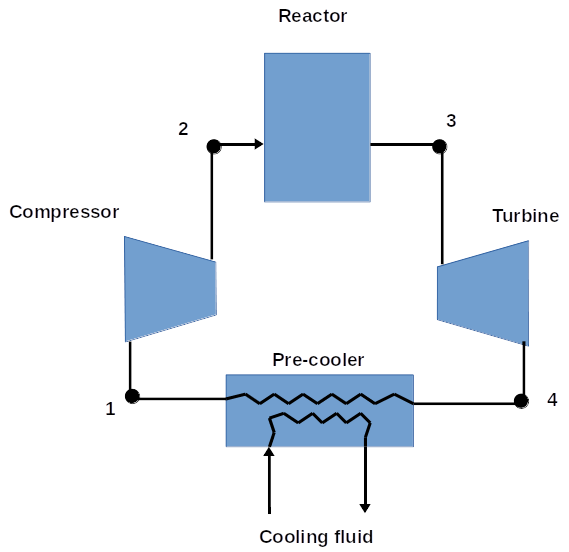
\includegraphics{simple_brayton.png}
\caption{A simple direct Brayton cycle for nuclear energy conversion.} 
\label{fig:simple_brayton}
\end{marginfigure}
\begin{enumerate}
\item isentropic compression ($ 1 \rightarrow 2$)
\item isobaric heat addition ($ 2 \rightarrow 3$)
\item isentropic expansion ($3 \rightarrow 4$)
\item isobaric heat rejection ($4 \rightarrow 1$)

\end{enumerate}
These are the same processes as a Rankine cycle; the difference is that the working fluid does not undergo a phase change during either heat addition or heat rejection; the working fluid is modeled as a compressible gas.  The temperature-entropy diagram for a non-ideal variation of the cycle is shown in Figure \ref{fig:simple_brayton_TS}.  For this, the compressor and turbine both are non-isentropic.
\begin{marginfigure}
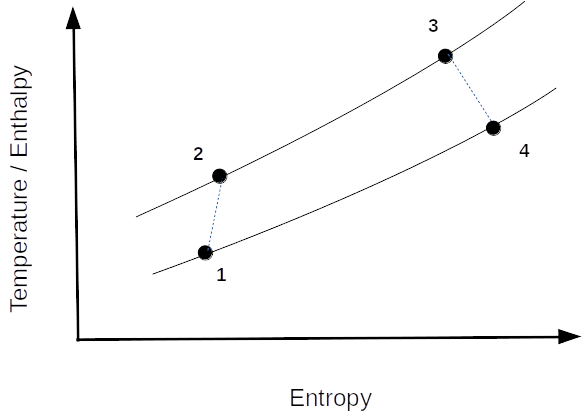
\includegraphics{simple_brayton_TS.png}
\caption{Temperature-Entropy diagram for a simple non-ideal Brayton cycle.}
\label{fig:simple_brayton_TS}
\end{marginfigure}

A more accurate representation of the cycle would also account for inevitable hydraulic losses as the working fluid flows through ducting and heat exchangers associated with the cycle.  For a Rankine cycle using water as the working fluid, these loss mechanisms are comparatively small but for Brayton cycle these losses are important and have a large impact on overall system thermodynamic performance.

\section{Analysis of Ideal Brayton Cycle - Constant Specific Heat}

If we assume the working fluid is an ideal gas in which the specific heat at constant pressure $(C_p)$ and constant volume $(C_v)$ are both assumed to be constant, an analytic solution method is feasible. We will model changes in enthalpy using the relationship given in Equation \ref{eq:IG_dh}.

\begin{equation}
\Delta h = C_p \Delta T
\label{eq:IG_dh}
\end{equation}

For isentropic processes a relationship exists between initial and final temperature of the working fluid, and the initial and final pressure of the working fluid. This relationship is given in Equation \ref{eq:IG_isentropic}.


\begin{equation}
\frac{T_f}{T_i} = \left(\frac{P_f}{P_i} \right)^{\frac{\gamma - 1}{\gamma}} = r_p^{\frac{P_f}{P_i}}
\label{eq:IG_isentropic}
\end{equation}


where $\gamma$ is the ratio of specific heats and $r_p$ is referred to as the ``pressure ratio.''\marginnote{\textbf{Note: }$\gamma = \sfrac{C_p}{C_v}$, and $r_p = \sfrac{P_f}{P_i}$}.  


\begin{example}
\textbf{Example:} Consider the a simple, ideal, closed, direct nuclear Brayton cycle.  Assuming the coolant is helium with $c_p=5.23 \text{ kJ/kg-}^{\circ}\text{K}$ and $\gamma=1.658$.  The maximum cycle temperature is 972 K and minimum temperature is 278 K.  The compressor pressure ratio is 4.0.  Find:
\begin{enumerate}
\item net specific work
\item thermal efficiency; and
\item back work ratio
\end{enumerate}
\end{example}

\begin{fullwidth}
\textbf{Solution:} 
Work of the isentropic compressor and turbine can be found by combining Equation \ref{eq:IG_dh} and Equation \ref{eq:IG_isentropic}.  

For the compressor we get:
$$w_c = h_1 - h_2 = C_p(T_1 - T_2) = C_p(T_1 - T_1 r_p^{\sfrac{\gamma - 1}{\gamma}}) = C_p T_1 (1 - r_p^{\sfrac{\gamma - 1}{\gamma}})$$
Applying the given numbers gives us:
$$w_c = (5.23 \text{kJ/kg-K})(273 \text{K})(1-4^{\sfrac{0.658}{1.658}}) = 1066.5 \text{kJ/kg}$$
For the turbine we get:
$$W_t = h_3 - h_4 = C_p(T_3 - T_4) = C_p(T_3 - T_3(\frac{1}{r_p})^{\frac{\gamma-1}{\gamma}}] = C_p T_3 [1 - (\frac{1}{r_p})^{\sfrac{\gamma-1}{\gamma}}]$$
which comes to:
$$w_t = (5.23 \text{kJ/kg-K})(972 \text{K})(1 - 0.25^{\frac{0.658}{1.658}}) = 2151.1 \text{kJ/kg}$$
net specific work is thus: $w_{\text{net}}=-1066.5 + 2151.1 = 1084.3 \text{kJ/kg}$.

\vspace{0.5cm}

We should calculate net specific heat added in order to compare with net work; for this we need values for the temperature at state points 2 and 4.  Using Equation \ref{eq:IG_isentropic} we get $T_2 = T_1 r_p^{\sfrac{\gamma-1}{\gamma}} = 278(4)^{\sfrac{0.658}{1.658}}=481.9$K and $T_4 = T_3 (\sfrac{1}{r_p})^{\sfrac{\gamma - 1}{\gamma}} = 972(0.25)^{\sfrac{0.658}{1.658}} = 560.7$K.  
Using these numbers with Equation \ref{eq:IG_dh} we get: $q_r = h_1 - h_4 = C_p(T_1 - T_4) = 5.23 \text{kJ/kg-K}(278 - 560.7) = -1478.5$kJ/kg and $q_s = h_3 - h_2 = C_p(T_3 - T_2) = 5.23 \text{kJ/kg-K}(972 - 481.9) = 2563.2$kJ/kg. 
Net specific heat added is, therefore: $q_{\text{net}} = q_s + q_r = 2563.1 - 1478.5 = 1084.7$kJ/kg which is very close to our calculated value for $w_{\text{net}}$.  

\vspace{0.5cm}
Thermal efficiency is given as $\eta_{th} = \sfrac{w_{\text{net}}}{q_s} = \sfrac{1084.7}{2563.2} = 0.423$ or 42.3 percent.

\vspace{0.5cm} 

The back work ratio is, by definition, the ratio of the magnitude of work supplied to the working fluid and the work extracted from the working fluid: $\text{BWR} = \sfrac{w_{\text{in}}}{w_{\text{out}}} = \sfrac{w_c}{w_t} = \sfrac{1066.5}{2151.1} = 0.496.$
\end{fullwidth}

\subsection{Discussion of Example}
A couple of points are worth noting on this example:
\begin{enumerate}
\item The analysis reveals a relatively high thermal efficiency.  This is owing in part to the ideal work processes and the neglect of hydraulic losses in heat exchanger components.
\item This result also reflects the good thermodynamic properties of helium as the working fluid for a Brayton cycle.  
\end{enumerate}
In future problems we will examine the performance of alternative working fluids as well as the impact of non-ideal components and hydraulic pressure losses on overall thermodynamic performance.

\section{Analysis with EasyProp}
When air, or any other polyatomic gas, is the working fluid it is common to take into account the variability of the specific heats as a function of temperature.  The thermodynamic properties available through EasyProp take such variability into account.



\begin{marginfigure}
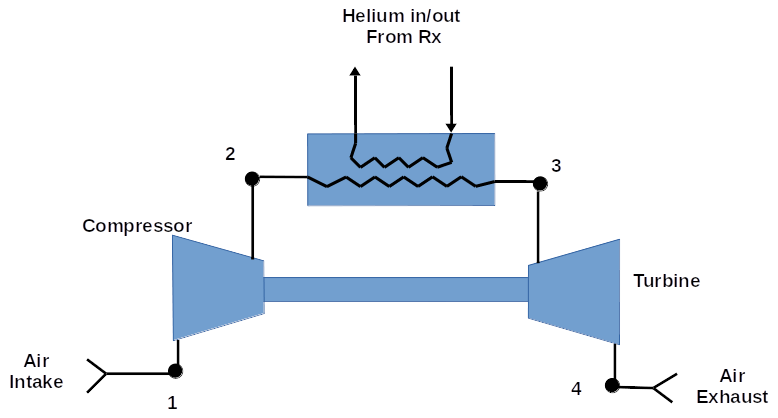
\includegraphics{simple_brayton_ex_schematic.png}
\caption{Open, indirect Brayton cycle.}
\label{fig:simple_brayton_ex_schematic}
\end{marginfigure}



\begin{example}
\textbf{Example:} A small modular reactor concept is proposed in which a helium-cooled, graphite moderated reactor transfers energy in a heat exchanger to an open Brayton cycle as depicted below.  A schematic is shown in Figure \ref{fig:simple_brayton_ex_schematic}. Air at 14.7 psia and 60$^{\circ}$F enters the compressor, passes through the heat exchanger at constant pressure and expands through a turbine that exhausts to the atmosphere.  The compressor has a pressure ratio of 14 and the turbine inlet temperature is 1600$^{\circ}$F. Compressor isentropic efficiency is 87\% and the turbine isentropic efficiency is 90\%.  

Find:

\begin{enumerate}
\item net specific work
\item cycle thermal efficiency; and
\item back work ratio
\end{enumerate}
\end{example} 

\newthought{This example considers} an indirect, open Brayton cycle that uses air for the working fluid.  The solution will be found using EasyProp with, in this case, the entirety of the analysis code included.  A state point table summarizing the thermodynamic properties after each process in the cycle  and numeric results are provided in Figure \ref{fig:simple_brayton_ex_sol}.

\begin{marginfigure}
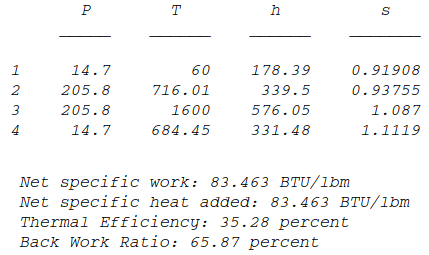
\includegraphics{simple_brayton_ex_results.png}
\caption{Numeric results}
\label{fig:simple_brayton_ex_sol}
\end{marginfigure}

\textbf{Solution:}
Full solution code is provided in the listing below.
\begin{lstlisting}
%% Open, Indirect, Air Brayton Cycle Example
clear
clc
close 'all'

%% Put EasyProp on Python path
% put location of EasyProp.py module on the python search path
if count(py.sys.path,' ') == 0  % <-- see if desired directory is on path
    insert(py.sys.path,int32(0),' '); %<-- if not; add it.
end

%% Initialize Fluid Property object
fluid = 'Air';
units = 'USCS';
air = py.EasyProp.simpleFluid(fluid,units);

%% Initialize state point arrays for Brayton Cycle
numSP = 4;
h = nan(numSP,1);
hs = nan(numSP,1);
s = nan(numSP,1);
ss = nan(numSP,1);
T = nan(numSP,1);
P = nan(numSP,1);

%% Problem Parameters
Pmin = 14.7; % psia, atmospheric pressure
Tin = 60; % F, inlet air temperature
r_p = 14;
r_e = 1/r_p;
T_turb_inlet = 1600; % F

eta_c = 0.87;
eta_t = 0.9;

%% Compute State Point Property Data
% state point 1
P(1) = Pmin;
T(1) = Tin;
h(1) = air.h_pT(P(1),T(1));
s(1) = air.s_pT(P(1),T(1));

% state point 2
P(2) = P(1)*r_p;
ss(2) = s(1);
hs(2) = air.h_ps(P(2),ss(2));
h(2) = h(1) - (h(1)-hs(2))./eta_c;
T(2) = air.T_ph(P(2),h(2));
s(2) = air.s_ph(P(2),h(2));

% state point 3
P(3) = P(2); %isobaric heat addition
T(3) = T_turb_inlet; % F, given
h(3) = air.h_pT(P(3),T(3));
s(3) = air.s_pT(P(3),T(3));

% state point 4
P(4) = P(3)*r_e;
ss(4) = s(3); 
hs(4) = air.h_ps(P(4),ss(4));
h(4) = h(3)-(h(3)-hs(4))*eta_t;
T(4) = air.T_ph(P(4),h(4));
s(4) = air.s_ph(P(4),h(4));

% display state point data neatly
SP = {'1','2','3','4'};
SP_table = table(P,T,h,s,'RowName',SP);
disp(SP_table);

%% First Law Analysis
w_c = h(1) - h(2);
w_t = h(3) - h(4);
w_net = w_c + w_t;

q_s = h(3) - h(2);
q_r = h(1) - h(4);
q_net = q_s + q_r;

assert(abs(w_net - q_net)<1,'Conservation of energy condition not met!');

fprintf('Net specific work: %g BTU/lbm \n',w_net);
fprintf('Net specific heat added: %g BTU/lbm \n',q_net);


eta_th = w_net/q_s;

fprintf('Thermal Efficiency: %5.2f percent \n',eta_th*100);

BWR = abs(w_c/w_t);
fprintf('Back Work Ratio: %5.2f percent \n',BWR*100);
\end{lstlisting}





\chapter{Lecture 11 - More Complex Brayton Cycles}
\label{ch:ch11}
\section{Objectives}
The objectives of this lecture are:
\begin{enumerate}
\item Discuss impact of pressure ratio on cycle thermal efficiency
\item Regeneration and Regenerator effectiveness
\item intercooling and reheat
\end{enumerate}

\section{Pressure Ratio and Thermal Efficiency}
For an ideal cycle (isentropic compressor/turbine and no hydraulic losses) thermal efficiency is related to compressor pressure ratio as follows:
\begin{marginfigure}
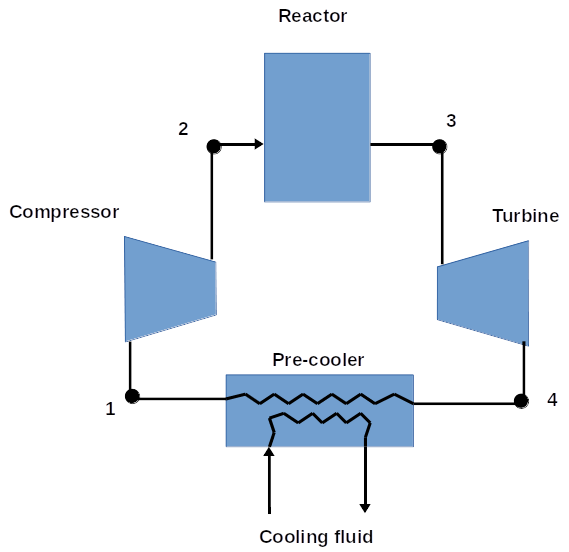
\includegraphics{simple_brayton.png}
\caption{Simple Ideal Brayton Cycle.}
\end{marginfigure}
\begin{align*}
\eta_{\text{TH}} &=\frac{w_{\text{net}}}{q_s} \\
                 &= \frac{C_p(T_3 - T_4) - C_p(T_2 - T_1)}{C_p(T_3 - T_2)} \\
                 &=\frac{(T_3 - T_2) - (T_4 - T_1)}{(T_3 - T_2)} \\
                 &=1 - \frac{T_4 - T_1}{T_3 - T_2} \\
                 &=1 - \frac{T_1(\sfrac{T_4}{T_1}-1)}{T_2(\sfrac{T_3}{T_2}-1)}
\end{align*}
If there are no pressure losses, then the pressure ratios for the compressor and turbine process are the same and $\sfrac{T_4}{T_1} = \sfrac{T_3}{T_2}$ so the last equality reduces to:
\begin{equation*}
\eta_{\text{TH}}=1 - \frac{T_1}{T_2}
\end{equation*}
Using our ideal gas relation for isentropic processes, $T_2 = T_1(r_p)^{\sfrac{(\gamma - 1)}{\gamma}}$ we obtain our final result in Equation \ref{eq:brayton_eff}.
\begin{equation}
\eta_{\text{TH}}=1 - \frac{1}{r_p^{\sfrac{(\gamma - 1)}{\gamma}}}
\label{eq:brayton_eff}
\end{equation}
For an ideal gas thermal efficiency increases for increasing pressure ratio. In principle this means we should be able to make thermal efficiency arbitrarily close to 100\% by increasing pressure ratio. In practice there are other considerations that need to be taken into account.

\section{Pressure Ratio and Net Specific Work}
\newthought{For many Brayton cycles} the pressure ratio affects achievable net specific work. This is because:
\begin{enumerate}
\item Real systems have limitations to the maximum temperature of the working fluid.  Some factors that lead to this limitation include:
\begin{enumerate}
\item material limits of the system piping and structural components
\item material limits of the heat source---such as nuclear reactor core outlet temperature limits---which, in order to add heat to the working fluid, are an upper bound to the maximum Brayton cycle system temperature.
\end{enumerate}
As pressure ratio increases, so does the temperature at the compressor discharge ($T_2$), so these maximum temperature limits impose a limit to the compressor pressure ratio.  Advances in material sciences offer the possibility of increasing these temperature limits over time but, for any concept, the designer has limited ability to influence this bound.
\item Real systems have limits to the minimum temperature of the working fluid.  This is dictated by the temperature of the thermal reservoir to which the cycle must reject heat in the pre-cooler.  This environmental temperature is generally outside of the control of the designer.  
\end{enumerate}
 
\begin{marginfigure}
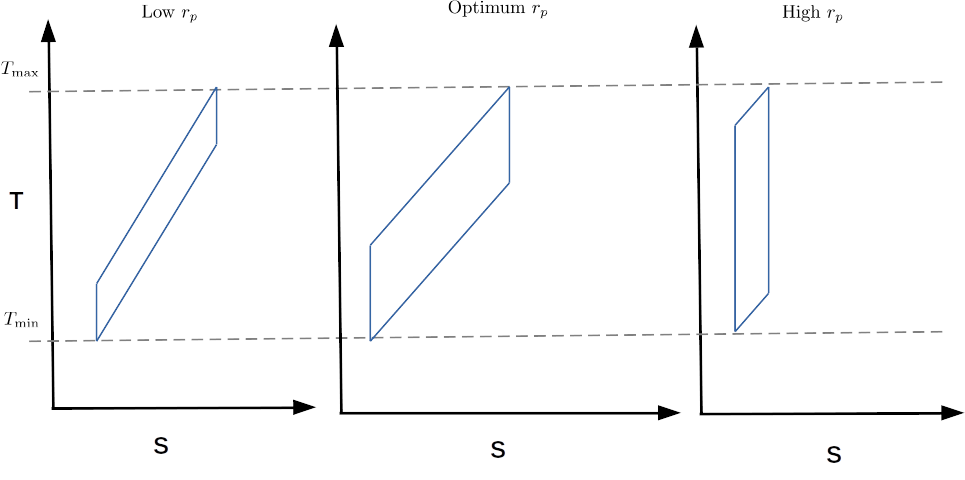
\includegraphics{brayton_wnet_vs_rp.png}
\caption{Effect of $r_p$ on $w_{\text{net}}$ for simple ideal Brayton cycles.}
\label{fig:wnet_vs_rp}
\end{marginfigure}
\newthought{These limits influence} the maximum net specific work that can be extracted from the working fluid for an ideal Brayton cycle. Figure \ref{fig:wnet_vs_rp} gives a qualitative feel for the influence of pressure ratio on net specific work for systems operating within material limits. Some key points:
\begin{itemize}
\item At low $r_p$, most of the added heat is simply rejected to the environment. 
\item At high $r_p$, the amount of heat that can be added to the working fluid is constrained by the temperature limit; thermal efficiency is high but, since $w_{\text{net}}$ is limited, the mass flow rate of the coolant must be higher to achieve a desired power output.
\item The optimum $r_p$ is a function of the working fluid. Figure \ref{fig:wnet_vs_rp_fluid} illustrates this for four typical Brayton cycle working fluids. 
\end{itemize}

\begin{marginfigure}
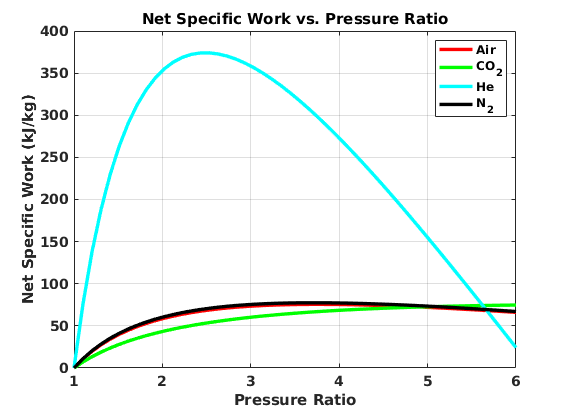
\includegraphics{Brayton_wnet_vs_rp_and_fluid.png}
\caption{Net specific work vs pressure ratio for common fluids.}
\label{fig:wnet_vs_rp_fluid}
\end{marginfigure}

\marginnote[0.5cm]{\textbf{Note:} looking at Figure \ref{fig:wnet_vs_rp_fluid}, which fluid is different from the others?}

\begin{itemize}
\item Reduced $w_{\text{net}}$ and increased $\dot{m}$ of working fluid may seem like a small price to pay for increased thermal efficiency but:
\begin{itemize}
\item Real systems will suffer hydraulic pressure losses that are proportional to $\dot{m}$
\item The thermal efficiency of a Brayton cycle is heavily impacted by those hydraulic pressure losses as we will see from our exercises.
\item Sadly a detailed treatment which connects all of the dots between pressure ratio, working fluid mass flow rate, and analysis of thermal efficiency including hydraulic pressure losses still needs to be brought into the scope of this class.
\end{itemize} 

\end{itemize}

\index{Brayton cycle, regeneration}
\section{Brayton Cycle with Regeneration}

\begin{marginfigure}
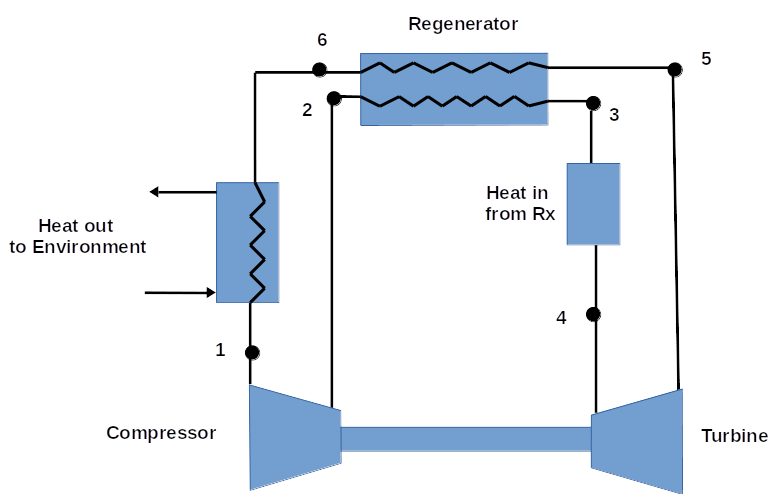
\includegraphics{brayton_regen.png}
\caption{Schematic of a regenerative Brayton cycle.}
\label{fig:brayton_regen}
\end{marginfigure}
\begin{marginfigure}
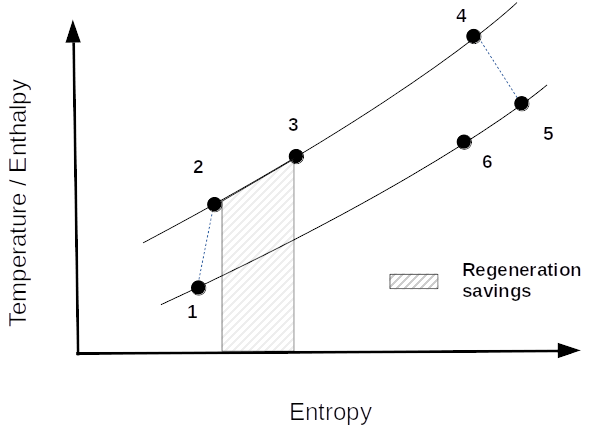
\includegraphics{brayton_regen_TS.png}
\caption{Reduced $q_s$ due to regeneration savings}
\label{fig:brayton_regen_TS}
\end{marginfigure}

\newthought{One obvious weakness} of the simple ideal Brayton cycle is the large amount of useful energy that gets rejected to the environment.  The working fluid at the turbine exhaust (state point 4) is at low pressure but its temperature remains high.  We can exploit the exergy contained in this high temperature fluid in a regenerator as illustrated in Figure \ref{fig:brayton_regen}.  Use of the regenerator reduces the amount of energy that need be added in the heat addition process.  This is illustrated in Figure \ref{fig:brayton_regen_TS}.



\index{regenerator effectiveness}
\newthought{We characterize the performance} of the regenerator with a parameter called \emph{regenerator effectiveness}.\marginnote[0.25cm]{\textbf{regenerator effectiveness:} the ratio of the actual enthalpy increase of the fluid on the low temperature side to the maximum theoretical enthalpy increase.}  The regenerator effectiveness for this cycle can be expressed as in Equation \ref{eq:regen_eff}.
\begin{equation}
\eta_{\text{reg}} = \frac{\Delta h_{\text{actual}}}{\Delta h_{\text{max}}} = \frac{h_3 - h_2}{h_5 - h_2}
\label{eq:regen_eff}
\end{equation}
Having a higher regenerator effectiveness is obviously desirable but is subject to limits.  Qualitatively speaking one increases regenerator effectiveness by:
\begin{itemize}
\item Increasing heat transfer surface area in the regenerator---e.g. make the regenerator bigger.
\item Enhancing heat transfer effectiveness in the regenerator. This might be done by:
\begin{itemize}
\item use materials with better conductive heat transfer properties
\item use convective heat transfer enhancements such as spiral grooves.  
\end{itemize}
\item use working fluids with better heat transfer properties.
\end{itemize}
With the exception of convective heat transfer enhancements which we will discuss in a later lecture, these considerations are beyond the scope of this course. Like isentropic efficiency data for pumps, compressors, and turbines, we will take regenerator effectiveness to be a given parameter.  \textbf{A typical value will be around 60\%.}

\section{Inter-cooling} \index{Brayton cycle, inter-cooling}
\begin{marginfigure}
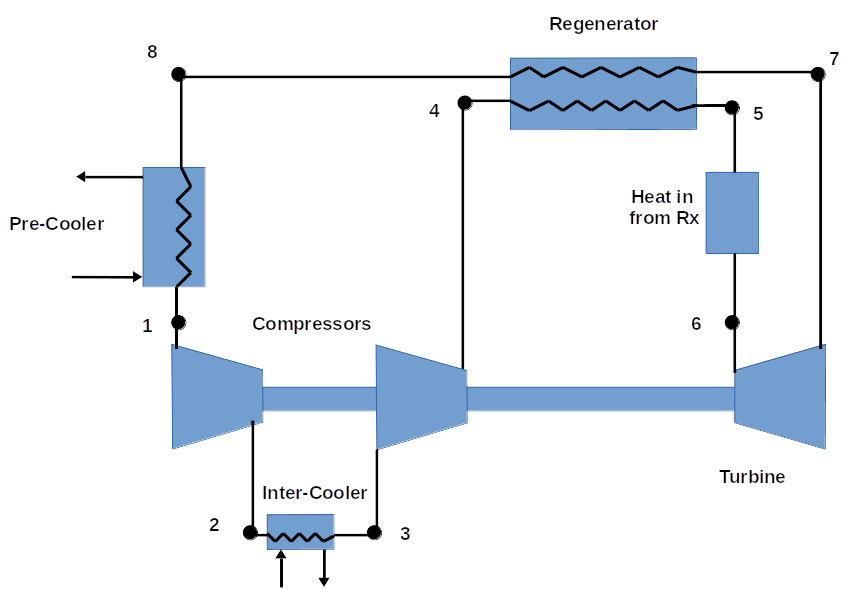
\includegraphics{brayton_regen_IC.png}
\caption{Brayton cycle with regeneration and inter-cooling.}
\label{fig:brayton_regen_IC}
\end{marginfigure}

\begin{marginfigure}
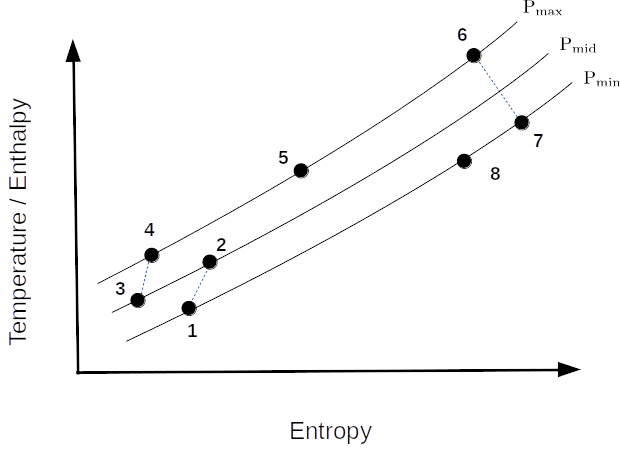
\includegraphics{brayton_IC_TS.png}
\caption{TS plot of a Brayton cycle with regeneration and inter-cooling.}
\label{fig:brayton_IC_TS}
\end{marginfigure}

\begin{marginfigure}
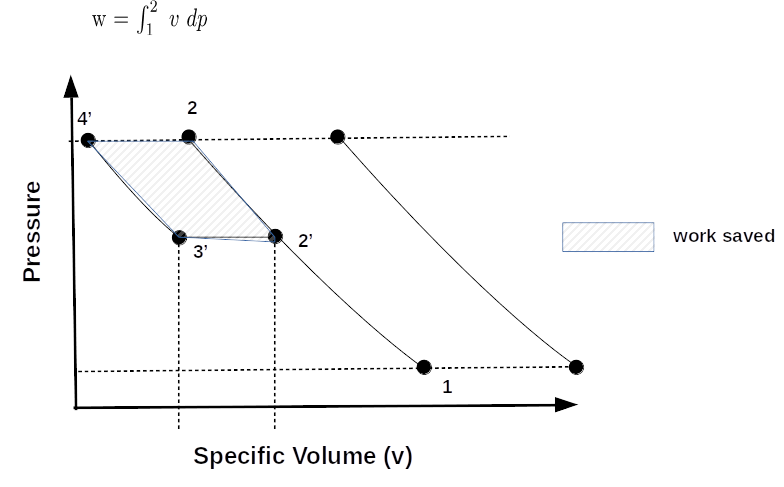
\includegraphics{brayton_IC_pv.png}
\caption{Work savings from inter-cooling.}
\label{fig:brayton_IC_pv}
\end{marginfigure}
\newthought{In addition to} using regeneration to reduce heat rejected, it is desirable to reduce the work required in the compression processes.  As characterized by the back work ratio, as much as half (or more!) of the turbine work for a Brayton cycle may be needed to power the compressor.  We can reduce the work required for compression by \emph{cooling} the working fluid part-way through the compression.  A Brayton cycle schematic with such an \emph{inter-cooler} is shown in Figure \ref{fig:brayton_regen_IC}. Heat extracted in the inter-cooler is normally rejected to the environment.  While it's traditional to show the temperature-entropy diagram---this is shown in Figure \ref{fig:brayton_IC_TS}---the work savings from inter-cooling is more easily seen from the $P-v$ diagram in Figure \ref{fig:brayton_IC_pv}. 



\newthought{A natural question} to ask is: How much of the compression should be done with the first compressor and how much with the second to get maximum work reduction?  It is a straight-forward but tedious task to show that, for isentropically ideal compressors working on ideal gasses with constant specific heats, you \emph{minimize overall compressor work if the pressure ratios for the compressors are the same.}  

\index{Brayton cycle, reheat}

\section{Brayton Cycle with Reheat}


\newthought{Another way to increase} the net specific work and thermal efficiency of a Brayton cycle is to include one or more stages of reheat.  A T-S diagram is shown in Figure \ref{fig:brayton_IC_RH_TS} and a schematic representation of such a cycle is illustrated in Figure \ref{fig:brayton_IC_RH}.
\begin{marginfigure}
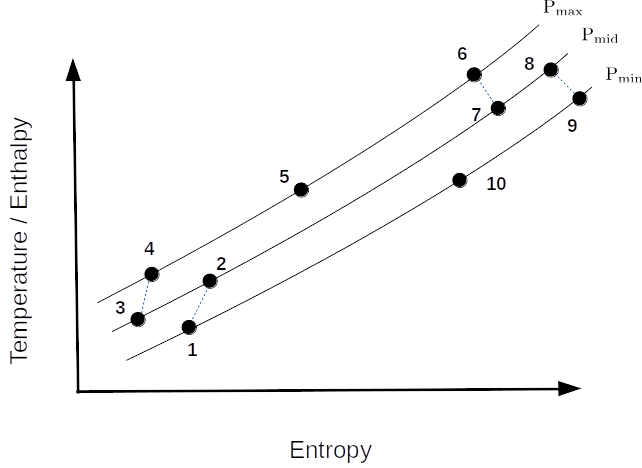
\includegraphics{brayton_IC_RH_TS.png}
\caption{T-S diagram for Brayton cycle with reheat.}
\label{fig:brayton_IC_RH_TS}
\end{marginfigure}

\begin{figure}
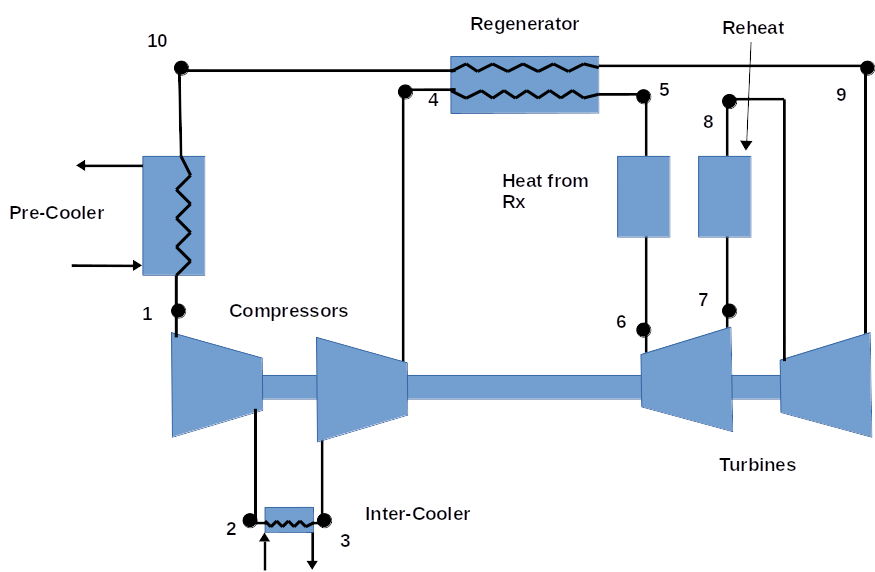
\includegraphics{brayton_IC_RH.png}
\caption{Brayton cycle with reheat.}
\label{fig:brayton_IC_RH}
\end{figure}

You should be asking the same question as with inter-cooling: how do I set the pressure ratios for the turbines such that I get maximum benefit from reheating?  Sadly I do not have a short answer to this question. To help you build some intuition on this, we will investigate this issue in our workshop assignments.



\chapter{Assignment \#4: Brayton Cycle Analysis}
\label{ch:ass4}

\begin{fullwidth}
\newthought{Use EasyProp} and MATLAB to analyze the following problems:

\begin{enumerate}
\item Air enters a simple open Brayton cycle at 14.7 psia and 85$^{\circ}$F.  Compressor pressure ratio is 5 and the isentropic efficiency of the compressor is 85\%.  Helium coolant from a Very High Temperature Reactor (VHTR) supplies heat to the air in a heat exchanger so that the inlet temperature to the turbine in the Brayton cycle is 1200$^{\circ}$F.  The turbine isentropic efficiency is 90\%.  Air exiting the turbine is discharged to the atmosphere at 14.7 psia.  Calculate:
\begin{enumerate}
\item Net specific work. [BTU/lb$_\text{m}$]
\item Thermal efficiency.
\item Mass flow rate needed for $5 \times 10^6$ BTU/hr power output. [lb$_\text{m}$/s]
\end{enumerate}

\vspace{1.0cm}

\item Consider the cycle described in Problem \#1.  While maintaining constant maximum and minimum temperature of 85$^{\circ}$F and 1200$^{\circ}$F respectively, constant isentropic efficiency of the compressor and turbine of 85\% and 90\% respectively, vary the compressor pressure ratio between 2 and 15.
\begin{enumerate}
\item Make plots of thermal efficiency and net specific work over that range of compressor pressure ratio.
\item Determine the pressure ratio for maximum thermal efficiency.
\item Determine the pressure ratio for maximum net work.
\end{enumerate}
Briefly explain your results in a short paragraph of approximately 250 - 500 words.

\vspace{1.0cm}

\item Consider again the cycle described in Problem \#1.  Instead of discharging the turbine exhaust directly to atmosphere, direct the turbine exhaust to a regenerator.  Turbine exhaust gases preheat the air discharged from the compressor prior to having heat added by the VHTR coolant.  Assume the regenerator effectiveness is 85\%.
\begin{enumerate}
\item Create a simple schematic of your cycle; label all state point numbers.
\item Calculate net specific work for the cycle. [BTU/lb$_{\text{m}}$]
\item Calculate the thermal efficiency of the cycle.
\end{enumerate}

\vspace{1.0cm}

\item Consider the cycle you have created for Problem \#3.  Study the performance as regenerator effectiveness is varied from 0\% to 100\%; make a plot of thermal efficiency versus regenerator effectiveness.  Briefly comment on your results (250 - 300 words) and verify that your results make sense.

\vspace{1.0cm}

\item Consider again the cycle described in Problem \#1.  Incorporate two-stage compression with an inter-cooler between stages.  Assume that the working fluid is cooled to 85$^{\circ}$F (at constant pressure) before entering the second compressor.  Consider three different cases for the pressure ratios of the two compressors:
\begin{enumerate}
\item Both compressors have the same compressor pressure ratio $(r_{p,1} = r_{p,2} = \sqrt{5})$.
\item $r_{p,1}=1.5$, $r_{p,2}= \sfrac{5}{1.5}$.
\item $r_{p,1} = \sfrac{5}{1.5}$, $r_{p,2}=1.5$.
\end{enumerate}
Calculate compressor work and thermal efficiency for each case.  Briefly comment on  your results. (\textbf{Note:} you need not do a second-law analysis on this cycle so there is no need to try and compute the state of the fluid that serves as the heat sink in the inter-cooler.)

\vspace{1.0cm}

\item Consider a Brayton cycle with inter-cooling, regeneration, and reheat.  Air enters the cycle at 14.7 psia, 85$^{\circ}$F.  Two stages of compressors are used, each with equal compressor pressure ratio, so that the overall pressure ratio is 5.  A regenerator is used with a regenerator effectiveness of 80\%.  After heat is added to a maximum temperature of 1200$^{\circ}$F, two turbines are used with re-heating between the two stages; the reheat procss is isobaric and the air temperature out of the reheater is 1200$^{\circ}$F.  Assume there are no hydraulic pressure losses within system components.  \textbf{Note:} As with the last problem, you need not evaluate state point properties of the helium coolant from the VHTR, nor need you analyze the state point properties for the heat sink of the inter-cooler.
\begin{enumerate}
\item Make a simple sketch of your system, being sure to identify all state points.
\item Vary the expansion ratio of the turbines as follows:
\begin{enumerate}
\item $r_{e,1} = r_{e,2} = \sqrt{5}$
\item $r_{e,1} = 1.5$, $r_{e,2} = \sfrac{5}{1.5}$
\item $r_{e,1} = \sfrac{5}{1.5}$, $r_{e,2} = 1.5$
\end{enumerate}
Calcualte net specific work and thermal efficiency for all three cases.  Briefly comment on your results (250 - 500 words).
\end{enumerate}

\end{enumerate}


\end{fullwidth}

\chapter{Lecture 12 - Supercritical CO$_{2}$ Brayton Cycles}
\label{ch:ch12}
\section{Objectives}
The objectives of this lecture are:
\begin{enumerate}
\item Illustrate the benefits of S-CO$_{2}$ Brayton cycles.
\item Show why regeneration is so important for S-CO$_{2}$ cycles.
\item Provide an alternative definition of regenerator effectiveness that one should use for supercritical gas power cycles.
\end{enumerate}

\section{CO$_{2}$ Brayton Cycles}

\newthought{When we introduced the Brayton cycle,} we used helium as the working fluid.  Indeed helium is a highly favored choice for numerous small modular reactor concept designs for high temperature reactors and we found that high cycle thermal efficiency could be obtained even with a simple (albeit ideal) Brayton cycle.  Helium, however, has some problems; some of these include:\cite{dostal2006supercritical}
\begin{itemize}
\item Helium is expensive.
\item Power conversion systems using helium can expect significant helium leakage through seals of rotating components and even welded boundaries.
\item Helium power cycle efficiency is more sensitive to regenerator effectiveness and fractional hydraulic pressure drops in plant components.
\item There is less experience World-wide in the use of Helium as a working fluid compared to air and CO$_{2}$.
\end{itemize}
For these reasons, for the time being, we will shift the focus of our attention to Brayton cycles using CO$_{2}$ as the working fluid.  

\newthought{Let us consider} a simple, ideal, closed Brayton cycle using CO$_{2}$ as the working fluid.  $P_{\text{max}}=2000$ kPa and $P_{\text{min}}=770$ kPa.  A schematic of the system and performance results are shown in Figure \ref{fig:co2_brayton_results}.

\begin{figure}
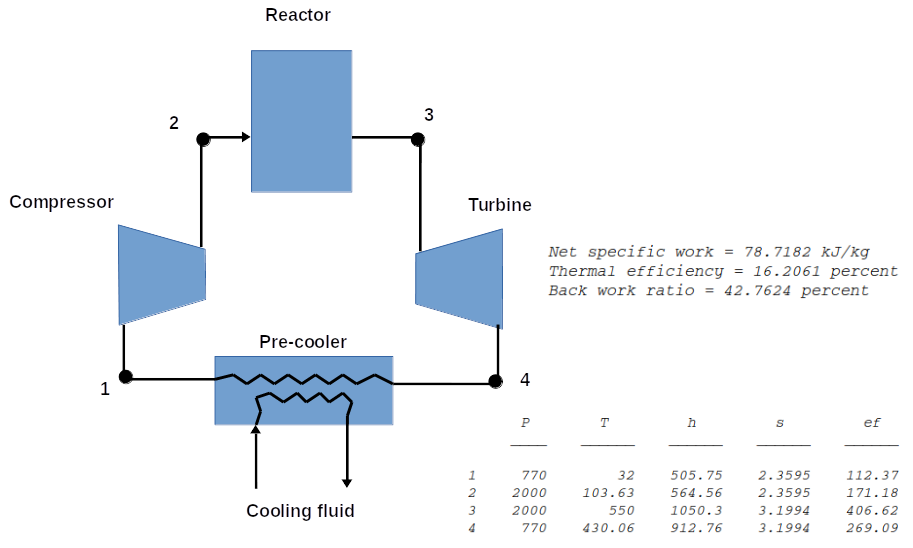
\includegraphics{co2_brayton_results.png}
\caption{Simple ideal Brayton cycle with CO$_{2}$}
\label{fig:co2_brayton_results}
\end{figure}

\newthought{From the state point table} it is evident that the fluid is still at a high temperature at the turbine exhaust; a considerable fraction of the energy/exergy provided by the reactor is rejected to the atmosphere. We can also see that the back work ratio is quite high. 

\subsection{Simple Supercritical CO$_{2}$ Brayton Cycle}

\begin{marginfigure}
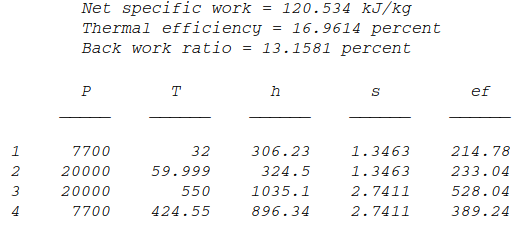
\includegraphics{sco2_brayton_results.png}
\caption{Analysis of simple Supercritical CO$_2$ Brayton Cycle}
\label{fig:sco2_brayton_results}
\end{marginfigure}

\newthought{Taking our lead} from the title of this lecture, we will examine how system performance changes when we increase system pressure above the critical pressure for CO$_{2}$ which is approximately 7.4 MPa while maintaining the same maximum temperature and pressure ratio.  The numerical results from the analysis are presented in Figure \ref{fig:sco2_brayton_results}. 

Note that the back work ratio has been drastically reduced. By pressurizing the CO$_2$ above the critical pressure, the specific volume is lower and the specific pump work has been reduced.  Still, the thermal efficiency is very low; we're still throwing away too much energy in the pre-cooler. A regenerator is definitely needed.

\subsection{Supercritical CO$_2$ Regenerative Brayton Cycle}
\newthought{We want to} reduce the amount of exergy rejected to the environment so we modify the cycle to add a regenerator.  We will choose a very optimistic regenerator effectiveness of 90\% while maintaining all other system parameters the same.\sidenote[][-0.5cm]{We will justify this optimisim by pointing to the expected heat transfer improvement with the CO$_{2}$ at high pressure and density.  We will also take comfort in the fact that the textbook assumes similar regenerator effectiveness for supercritical CO$_{2}$ cycles.}  A schematic of the cycle and analysis results are provided in Figure \ref{fig:sco2_brayton_regen_results1}
\begin{figure}
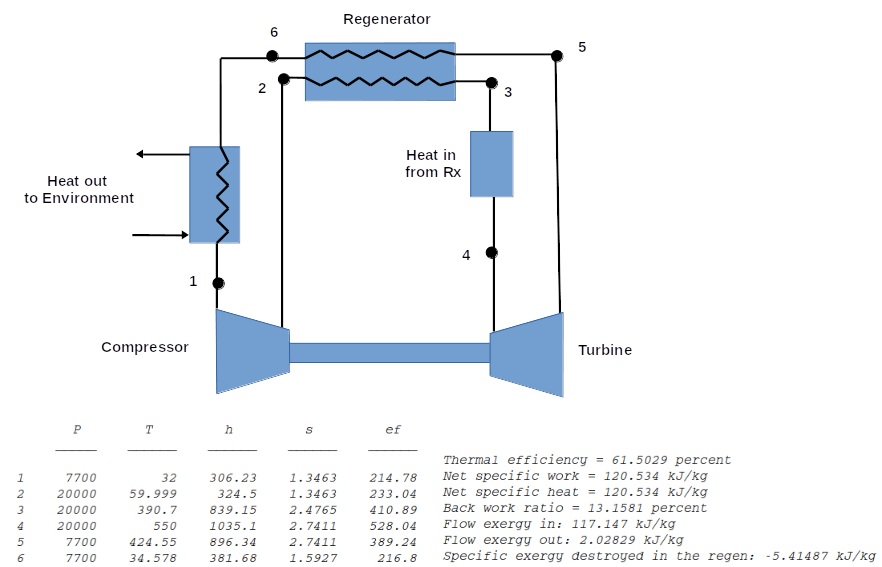
\includegraphics{sco2_brayton_regen_results1.png}
\caption[][1cm]{Regenerating S-CO$_{2}$ cycle.}
\label{fig:sco2_brayton_regen_results1}
\end{figure}

\newthought{As the results indicate,} adding regeneration did nothing to change net specific work, it's still at 120.5 kJ/kg, but recapturing that otherwise wasted energy, according to the analysis results in thermal efficiency increasing to over 61\%.(!!)  Before popping open the Champagne we should review the results of the exergy analysis.\sidenote{Before looking at the numbers repeat to yourself: ``\emph{Exergy} in minus \emph{exergy} out equals \emph{exergy} transfered through work plus \emph{exergy} destroyed.''} In round numbers, specific flow exergy passed in to the working fluid from the reactor is 117 kJ/kg, exergy rejected to the environment in the pre-cooler is a mere 2 kJ/kg; think of this as 115 kJ/kg of exergy being provided to the cycle for use.  But somehow we extracted 120 kJ/kg of specific work!?!  The explanation, and the sore thumb that should stick out at you when you examine the results, is the \underline{\emph{negative}} specific exergy destruction rate calculated for the regenerator.  What happened?

\newthought{The problem} is contained in our definition of regenerator effectiveness; not that it is necessarily too high, but that it is inadequate for this problem involving a fluid above its critical pressure.  Recalling from a previous lecture, we defined the regenerator effectiveness as:

\begin{equation}
\eta_{\text{reg}} = \frac{\Delta h_{\text{actual}}}{\Delta h_{\text{max}}} = \frac{h_3 - h_2}{h_5 - h_2}
\label{eq:regen_eff2}
\end{equation}   
but this formulation leaves out a key piece of physics: heat transfer, in a regenerator or elsewhere, is driven by temperature differences; the equation above only considers enthalpy values. Temperatures at the inlets and outlets of the regenerator for this analysis are shown in Figure \ref{fig:regen_temp_bad}. Note that the temperature at state point 6 (regenerator hot side outlet) is \underline{\emph{lower}} than state point 2 (cold side inlet).  This is obviously a violation of the 2nd law of thermodynamics.
\begin{marginfigure}
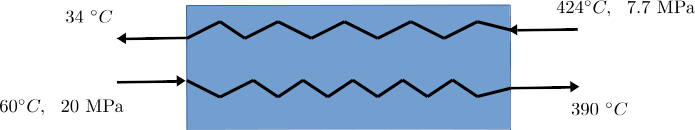
\includegraphics{regen_temps_bad.png}
\caption{Regenerator temperatures.}
\label{fig:regen_temp_bad}
\end{marginfigure}
We can re-connect enthalpy with temperature by using the specific heat at constant pressure, $C_p$.  Using this we can re-write Equation \ref{eq:regen_eff2} as:
\begin{equation}
\eta_{\text{reg}}=\frac{C_p(T_3 - T_2)}{C_p(T_5 - T_2)}
\label{eq:regen_eff3} 
\end{equation}

\begin{marginfigure}
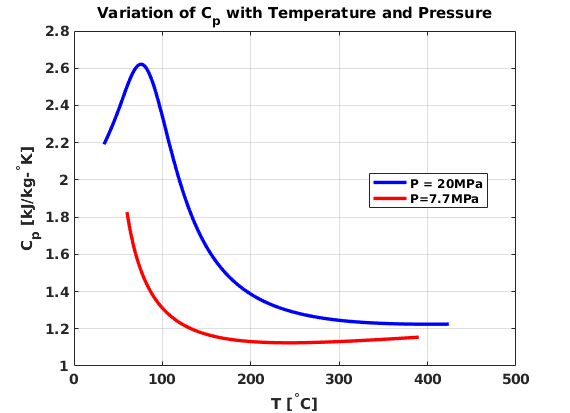
\includegraphics{variation_of_Cp_sco2_brayton_regen.png}
\caption{Variation of $C_p$ within the regenerator.}
\label{fig:cp_var}
\end{marginfigure}

This does not look like a great leap forward but we can now see that Equation \ref{eq:regen_eff3} leaves another detail out: the specific heat is \underline{not} constant.  A plot of specific heat at constant pressure for the high pressure and low pressure side of the regenerator is shown in Figure \ref{fig:cp_var}. 

An improvement can be made by refining our definition of regenerator effectiveness further\cite{bergman2011introduction} as follows:
\begin{equation}
\eta_{\text{reg}}=\frac{q}{q_{\text{max}}}=\frac{C_c(T_{c,o}-T_{c,i})}{C_\text{min}(T_{h,i}-T_{c,i})} = \frac{C_h(T_{h,i}-T_{h,o})}{C_\text{min}(T_{h,i}-T_{c,i})}
\label{eq:regen_eff4}
\end{equation}
where $C_c$ and $C_{\text{min}}$ refer to the specific heat at constant pressure for the cold stream and the minimum specific heat at constant pressure respectively.  But what is a good choice for either $C_c$ or $C_h$? ---they both change significantly over the temperature range of interest.
\begin{marginfigure}
\includegraphics{regen_t_schm.png}
\caption{Regenerator schematic}
\label{fig:regen_t_schm}
\end{marginfigure}

\newthought{The method we will use} is based on techniques described in a technical report from MIT\cite{dostal2004supercritical} and is given in Equation \ref{eq:regen_eff_sc}.

\begin{equation}
\eta_{\text{reg}} = \frac{h_3 - h_2}{h_5 - h_{P_6,T_2}} = \frac{h_5 - h_6}{h_5 - h_{P_6,T_2}}
\label{eq:regen_eff_sc}
\end{equation}
where $h_{P_6,T_2}$ is the enthalpy evaluated at the pressure of state point 6 (low pressure outlet), but the temperature at state point 2 (low temperature inlet).  This ensures that the denominator of Equation \ref{eq:regen_eff_sc} represents a maximum enthalpy change. 
\subsection{Supercritical CO$_{2}$ Regenerative Cycle Revisited}
Using this new method the cycle will be re-analyzed with all of the same parameters as before.  The results are presented in Figure \ref{fig:sco2_brayton_regen_results2}.  Once again, as expected, there is no change to the net specific work.  For this analysis, the thermal efficiency is a respectable 37.7\% and there is no negative exergy destruction.
\begin{marginfigure}
\includegraphics{sco2_brayton_regen_results2.png}
\caption{Regenerated S-CO$_{2}$ results with revised $\eta_{\text{reg}}$}
\label{fig:sco2_brayton_regen_results2}
\end{marginfigure}  
\newthought{You should note} the fairly high value of exergy destruction for the regenerator; particularly considering the optimistic regenerator effectiveness that we assumed.  Recall that exergy destruction is how we quantify irreversibility, and for heat transfer processes such as what occurs in the regenerator, irreversibility comes from transferring heat across temperature gradients.\sidenote[][-0.5cm]{Of course you need at least an infinitesimal temperature gradient to transfer heat; reversible heat transfer must take place across such an infinitesimal temperature gradient.} Plotting, as we did before, the temperatures at the inlets and outlets of the regenerator in Figure \ref{fig:regen_temps_good}, we get some idea as to the source of the extensive exergy destruction. Note the high differential temperature between the fluids at the right end of the regenerator as well as the significantly different change in temperature for the low- and high-pressure fluids respectively.
\begin{marginfigure}
\includegraphics{regen_temps_good.png}
\caption{Regenerator temperatures with revised effectiveness.}
\label{fig:regen_temps_good}
\end{marginfigure}
\newthought{The variation in temperature} change can be better understood in light of the variation of $C_p$ as shown before in Figure \ref{fig:cp_var}. On the high-pressure side, especially at lower temperatures, $C_p$ is much higher than it is at high temperature and low-pressure side.  This means that, if we have the same mass flow rate of working fluid on both the low- and high-pressure side of the heat exchanger, we will not be able to avoid having large differences in the temperature change.

A resolution to this issue will be introduced in the next lecture.  We will break the regenerator up into two stages: a low temperature regenerator and a high temperature regenerator.  In the low temperature regenerator, where the variation in $C_p$ between the fluids is greatest, we will reduce the mass flow rate on the high-pressure/low-temperature side.  This will allow the temperature changes on each side of the regenerator to be better matched.  Overall this scheme will result in effective regeneration with reduced exergy destruction and correspondingly improved efficiency.


\chapter{Lecture 13 - Recompressing, Regenerating S-CO$_{2}$ Cycle}
\label{ch:ch13}
\section{Objectives}
The objectives of this lecture are:
\begin{enumerate}
\item Give a detailed description of the analysis method for the RRS-CO$_{2}$ Brayton cycle
\item Discuss the MATLAB implementation of the solution
\end{enumerate}

\index{Brayton cycle, recompressing regenerating S-CO$_{2}$}
\section{Recompressing Regenerating S-CO$_{2}$ Brayton Cycle}
\newthought{A schematic of this cycle} is given in Figure \ref{fig:rrsco2_schematic}. In order to better match the temperature change on the cold- and hot- side of the regenerators, a portion of the working fluid bypasses the pre-cooler, compressor and low-temperature regenerator; instead it is recompressed and mixed with fluid leaving the low-temperature regenerator at state point 3.  The combined flow is pre-heated in the high-temperature regenerator before heat addition from the reactor.


\begin{figure}
\includegraphics{rrsco2_schematic.png}
\caption{Schematic RR S-CO$_{2}$ Brayton cycle.}
\label{fig:rrsco2_schematic}
\end{figure}

\newthought{Compared to } some of the more complex Rankine cycles analyzed in earlier lectures, this cycle is relatively simple with only 8 state points.  Still, there are some challenges to be overcome.  Let us suppose that we know the minimum and maximum pressure and temperature for the working fluid; we know (or can assume appropriate values for) the isentropic efficiency of the turbine and both compressors and we can assume a value of regenerator effectiveness for both the low- and high-temperature regenerators.
\begin{itemize}
\item With the aforementioned given and assumed data, we should be able to calculate thermodynamic properties at state point 1 and 2 along with 5 and 6. 
\item If we do not know the flow fraction $f$ of working fluid going through the pre-cooler then we cannot calculate the temperature or enthalpy of state point 3;
\item Without knowing the temperature or enthalpy of state point 3, we cannot calculate properties of state point 4, 7, or 8 either.
\end{itemize}
We have a total of 5 unknown properties---f, and the enthalpy/temperature of state points 3,4,7, and 8---and thus need to develop 5 independent relationships.  As with previous cycles, these equations in general will be non-linear and values of the dependent variables need to be constrained to ensure a physically meaningful solution.  We will form these equations using the following relationships:\marginnote[1.5cm]{\textbf{Note: }The equations are all re-arranged in the MATLAB code to facilitate use with FMINCON.  

Partial MATLAB code listing provided for clarity/completeness. A full MATLAB script to carry out this analysis is provided in the appendices.}
\begin{enumerate}
\item Low-temperature regenerator effectiveness:
$$\eta_{\text{LTR}} = \frac{h_7 - h_8}{h_7-h_{(P_8,T_2)}}$$
\begin{lstlisting}
%f = [flow fraction, h(3), h(4), h(7), h(8)]
gas = py.EasProp.simpleFluid('CO2','SI');
LTR_eff_eq = @(f) eta_LTR*(f(4) - ...
    gas.h_pT(P(8),T(2)))-(f(4)-f(5));
\end{lstlisting}

\item High-temperature regenerator effectiveness:
$$\eta_{\text{HTR}} = \frac{h_6 - h_7}{h_6 - h_{(P_7,T_2)}}$$
\begin{lstlisting}
%f = [flow fraction, h(3), h(4), h(7), h(8)]
HTR_eff_eq = @(f) eta_HTR*(h(6) - ...
    gas.h_pt(P(7),gas.T_ph(P(3),f(2))))-(h(6)-f(4));
\end{lstlisting}

\item Low-temperature regenerator energy balance:
$$f(h_3 - h_2) = h_7 - h_8$$
\begin{lstlisting}
%f = [flow fraction, h(3), h(4), h(7), h(8)]
LTR_ebal = @(f) f(1)*(f(2)-h(2))-(f(4)-f(5));
\end{lstlisting}

\item High-temperature regenerator energy balance:
$$h_4 - h_3 = h_6 - h_7$$

\begin{lstlisting}
%f = [flow fraction, h(3), h(4), h(7), h(8)]
HTR_ebal = @(f) (f(3)-f(2) - (h(6)-f(4));
\end{lstlisting}
\item The last relationship will be that the state of the fluid at exit from the low-temperature regenerator is the same as the state of the fluid discharged from the re-compressor.  On the schematic, both of these flows correspond to state point 3:
$$h_3 = h_8 - \frac{h_8 - h_{3s}}{\eta_{RC}}$$
where the left hand side is derived from a standard analysis of compressor work for the re-compressor.  Note for this equation, we do not know $h_{3s}$ and we do not want to add it to our list of unknown variables.  Instead we will re-express $h_{3s}$ in terms of what we do know along with existing unknowns:
$$h_{3s} = h_8 - \frac{h_8 - (h_8 - \overbrace{h(P_3,\overbrace{s(P_8,h_8)}^{s_8})}^{h_{3s}})}{\eta_{RC}}$$

\begin{lstlisting}
%f = [flow fraction, h(3), h(4), h(7), h(8)]
sp3_ident = @(f) f(5) - ...
    (f(5) - gas.h_ps(P(3),gas.s_ph(P(8),f(5))))/eta_rc - f(2);
\end{lstlisting}


\end{enumerate}
The five equations are then combined into a single balance equation for use with FMINCON.

\begin{lstlisting}
balance = @(f) abs(LTR_eff_eq(f)) + abs(HTR_eff_eq(f)) + ...
    abs(LTR_ebal(f)) + abs(HTR_ebal(f)) + abs(sp3_ident(f));
\end{lstlisting}

\newthought{We also need} to provide constraints to help ensure that FMINCON arrives at a physically meaningful solution. A table of possible constraints and starting values are provided in Table \ref{tb:rrsco_constraints}. These are encoded in MATLAB as follows:
\begin{margintable}
\begin{tabular}{lc}
\toprule
Constraint & Starting Value \\
\midrule
$0 \le f \le 1$ & 0.5 \\
$h_2 \le h_3 \le h_6$ & $h_2$ \\
$h_2 \le h_4 \le h_5$ & $h_5$ \\
$h_1 \le h_7 \le h_6$ & $h_6-1$ \\
$h_2 \le h_8 \le h_6$ & $h_2$ \\
\bottomrule
\end{tabular}
\caption{Constraints and starting values for cycle analysis.}
\label{tb:rrsco_constraints}
\end{margintable}

\begin{lstlisting}
%f = [flow fraction, h(3), h(4), h(7), h(8)]
lbound = [0 h(2) h(2) h(1) h(2)];
ubound = [1 h(6) h(5) h(6) h(6)];
Xo = [0.5 h(2) h(5) h(6)-1 h(2)];
\end{lstlisting}

\subsection{Results}
\newthought{As a reminder,} our goal was to reduce exergy destruction in the regenerator for a supercritical CO$_{2}$ Brayton cycle and thereby increase cycle thermal efficiency.  Results of the analysis are shown in Figure \ref{fig:rrsco2_results}. 
\begin{marginfigure}
\includegraphics{rrsco2_results.png}
\caption{Calculated results for RR S-CO$_{2}$ cycle.}
\label{fig:rrsco2_results}
\end{marginfigure}
We can see that the thermal efficiency is increased to 48.3\% and that the temperature differences at each side of the regenerators is reduced.  The largest differential temperature is at the high-temperature regenerator with state points 4 and 6 roughly 60 degrees different. It corresponds, therefore that the higher rate of exergy destruction is in the high-temperature regenerator.  The net specific work (and heat) is reduced because the specific work of the re-compressor is elevated since it is compressing working fluid that has not been pre-cooled.  



\chapter{Lecture 14 - Combined Cycles}
\label{ch:ch14}
\section{Objectives}
The objectives of this lecture are:
\begin{enumerate}
\item Describe an example combined cycle and illustrate key analysis methods
\item Illustrate incorporation of hydraulic pressure drops in a Brayton cycle.
\end{enumerate}

\index{Combined cycle}
\section{Combined Cycle by Example}
\newthought{One approach to} improving the thermal efficiency of the nuclear energy conversion process is to combine Brayton and Rankine cycles.  This is similar in concept to a regenerated Brayton cycle in that waste heat remaining after expansion of the working fluid through a turbine is recovered in some way.  Rather than using the energy to pre-heat the working fluid as in a regenerative Brayton cycle, the high temperature gasses are used as heat input to an entirely different thermodynamic cycle.  One such cycle\cite{forsberg2014meeting} is illustrated in the schematic in Figure \ref{fig:FHR_schematic}.  Key system parameters are summarized in Table \ref{tab:FHR_params}.  State point property data are tabulated in Figure \ref{fig:combined_cycle_SPT}.

\newthought{One notable feature} of this analysis is the inclusion of hydraulic pressure losses.  In previous cycle analyses, it was assumed either explicitly or implicitly that heat transfer processes in a Brayton cycle would take place at constant pressure.  In reality, viscous flow through complex heat exchanger geometry results in frictional pressure drops.  



\begin{figure}
\includegraphics{FHR_schematic.png}
\caption{Schematic of a FHR combined cycle}
\label{fig:FHR_schematic}
\end{figure}

\begin{margintable}
\begin{tabular}{lc}
\toprule
Property & Value \\
\midrule
$T_{\text{atm}}$ & 15$^{\circ}C$ \\
$P_{\text{atm}}$ & 101.3 kPa \\
$T_{\text{max}}$ & 770$^{\circ}C$ \\
$T_{\text{exh,air}}$ & 250$^{\circ}C$ \\
$r_{p}$ & 17 \\
$r_{e1}$ & 4 \\
$\eta_T$ & 0.92 \\
$\eta_c$ & 0.89 \\
$eta_p$ & 0.80 \\
\bottomrule
\end{tabular}
\caption{FHR Parameters}
\label{tab:FHR_params}
\end{margintable}

\begin{figure}
\includegraphics{combined_cycle_SPT.png}
\caption[][5cm]{State point property data for FHR.}
\label{fig:combined_cycle_SPT}
\end{figure}

Take for example air flow into the compressor.  Air is drawn from the atmosphere, here assumed to be at standard temperature and pressure, through inlet ducting which, besides directing air flow to the compressor inlet would perform other essential functions such as preventing the introduction of harmful foreign objects into the machine. It should be clear that the fluid arriving at state point 1 will have lost some energy in the process of traversing the dampers, filters, and various duct work. That energy loss will be manifest as a reduction in static pressure.  As is evident from the state point table, the pressure at state point 1 is listed as 100.3 kPa---1 kPa lower than atmospheric pressure.  

Similarly, air flowing from the compressor discharge through the heat exchanger between state points 2 and 3 cannot be expected to pass through the complex heat exchanger geometry without some flow-energy losses.  For this problem, the pressure loss $\Delta P_{HX} = P_3 - P_2 = 10$kPa.  In upcoming lectures we will examine techniques for quantifying hydraulic pressure losses in the context of diabatic flows such as this one.

For the purposes of lecture and associated homework problems, we will take hydraulic pressure losses to be given parameters.  The losses will be expressed either as:
\begin{enumerate}
\item fixed given $\Delta P$ as with the two cases just described; or
\item a fractional pressure drop where the $\Delta P$ for a given process will be given as a fraction of the state point pressure at the process inlet. 
\end{enumerate}
With this methodology it is often possible and preferable to compute all state point pressures first before determining all other state point properties.

\newthought{The hydraulic pressure drops} have a significant effect on net specific work and thermal efficiency.  If, as we have done up until now, we assumed no hydraulic pressure losses throughout the system, the net specific work and thermal efficiency would be 324.4 kJ/kg and 44.7\%.  Including pressure losses, net specific work is 300.5 kJ/kg and thermal efficiency is only 41.4\%.

\subsection{Analysis of Combined Cycle}
There are a few details to the analysis of a combined cycle that are best communicated simply by doing the calculations.  

\begin{enumerate}
\item What is the ratio of the air and steam mass flow rates?

This is determined through an energy balance for the heat recovery steam generator expressed in Equation \ref{eq:ebal_hrsg}

\begin{equation}
\dot{m}_a (h_6 - h_7) = \dot{m}_s (h_{10}-h_9)
\label{eq:ebal_hrsg}
\end{equation}
For this problem, therefore:
$$ \frac{\dot{m}_s}{\dot{m}_a} = \frac{h_6 - h_7}{h_{10}-h_9}$$

\item What is the net specific work for this cycle?

In this case, we need to be a bit more specific about what we mean by ``specific work.'' Normally the specific work is the power divided by the mass flow rate of the working fluid; but in this cycle we have two different working fluids with generally different flow rates.  In order to perform a consistent analysis of the cycle we should define specific work to be power per unit mass flow rate of \emph{one} of the working fluids; for this cycle we will choose the air in the Brayton cycle is the reference working fluid.

\begin{align*}
w_{\text{net}} &= \frac{\dot{W}}{\dot{m}_a} \\
               &= w_c + w_{T_1} + w_{T_2} + w_{T_3} + w_p \\
&=(h_1 - h_2) + (h_3 - h_4) + (h_5 - h_6) + \frac{\dot{m}_s}{\dot{m}_a}(h_{10}-h_{11}) + \frac{\dot{m}_s}{\dot{m}_a}(h_8 - h_9)\\ 
\end{align*}

\item What is the net specific heat added?

For this cycle, heat is added only in the processes from state points 2 to 3 and 4 to 5.\sidenote{\textbf{Question:} Why do you not count the heat exchanged in the heat recovery SG?}  Since air is the only working fluid involved in these processes, this calculation is carried out as before:

$$q_s = (h_3 - h_2) + (h_5 - h_4)$$

\item What is the cycle thermal efficiency?

Since we have taken care to consistently calculate both the net specific heat added and the net specific work in terms of the mass flow rate of air, we can compute thermal efficiency in the usual way:

$$\eta_{\text{TH}} = \frac{w_{\text{net}}}{q_s}$$

\item What would the thermal efficiency be without the Rankine ``Bottoming'' cycle?

For this calculation we would simply eliminate the specific work of the Rankine cycle turbine and pump from the net work calculation.

\end{enumerate}


\chapter{Assignment \#5: Advanced Brayton Cycle \& Combined Cycle Analysis}
\label{ch:ass5}

\newthought{Use EasyProp} and MATLAB to solve the following problems:

\begin{fullwidth}
\begin{enumerate}
\item The Marine Gas Cooled Reactor was proposed by General Atomics to the Atomic Energy Commission in 1961.  The design concept used a closed, direct, Brayton cycle to produce power. The Brayton cycle includes two compressors (with inter-cooling), a regenerator, and one turbine.  The working fluid is helium, the maximum helium temperature is 1300$^{\circ}$F, the minimum temperature is 100$^{\circ}$F, and the minimum pressure is 450 psia.  The isentropic efficiency of the compressors are each 85\% and the isentropic efficiency of the turbine is 90\%.  The regenerator effectiveness is assumed to be 90\%.  The inlet temperature to both compressors is 100$^{\circ}$F and the pressure ratios of the compressors are equal.
\begin{enumerate}
\item Make a simple sketch of the cycle labeling all state points and given information.
\item Find the thermal efficiency if $r_{p,1} = r_{p,2}=2.0$
\item Find the pressure ratio that gives the maximum thermal efficiency along with the thermal efficiency thus obtained; and
\item Using the pressure ratio that gives maximum thermal efficiency, find the helium flow rate [lb$_{\text{m}}$/s] and net power output [MW] if the thermal output of the reactor is 100 MW. (\textbf{Note:} 1 MW = $3.41 \times 10^6$ BTU/hr)
\end{enumerate}

\vspace{1.0cm}
\item Consider the cycle described in problem \#1.  Assume that there are hydraulic pressure losses for each heat exchanger equal to 2\% of the incoming pressure (e.g. $P_{\text{out}} = 0.98 \times P_{\text{in}}$); pressure losses across the reactor is 5\% of the incoming pressure.  What is the maximum thermal efficiency, helium flow rate, and net power output for 100 MW (thermal) reactor power output if hydraulic losses are included?  Investigate the individual impact of pressure loss in each component and write a short discussion of your findings. (\textbf{Note:} \emph{In your analysis you should consider determining all state point pressures first since ther will be, in general, no simple relationship between the compresor pressure ratios and the turbine expansion ratio.  This is owing to the pressure drops in the regenerator (both low temperature and high temperature side), reactor and pre-cooler.  Assume that, under all conditions, minimum system pressure is constant at 450 psia})

\vspace{1.5 cm}

\item Consider a closed, direct Brayton cycle.  Helium at 900 psia at 1500$^{\circ}$F leaves a High Temperature Gas-cooled Reactor (HTGR) and enters a turbine where the helium is expanded down to 1000 psia.  The helium exiting the turbine is used as the heat source in a Rankine cycle; the helium exits the boiler at 300$^{\circ}$F and then enters a compressor.  The steam produced in the boiler is expanded in a turbine to 1 psia and exhausted into a condenser which rejects wasted heat and delivers saturated liquid to a pump.  The pressure loss of the helium in the boiler and HTGR is 10 psia in each component.  For the Rankine cycle, assume that isobaric heat transfer occurs in the boiler and condenser.  The isentropic efficiency of all pumps, compressors, and turbines is 100\%. (\textbf{Hint:} consider using the EasyProp function ``P\_sT'' to get the turbine exhaust pressure.)

\begin{enumerate}
\item Draw a simple sketch of the system indicating given temperature and pressure data.
\item What is the ratio of helium mass flow rate and steam mass flow rate: $\frac{\dot{m}_{\text{steam}}}{\dot{m}_{\text{helium}}}$
\item What is the compressor pressure ratio for the compressor in the Brayton cycle?
\item What is the net work from the Rankine cycle and Brayton cycle  per unit mass flow rate of helium in BTU/lb$_{\text{m}}$?
\item What is the thermal efficiency of the combined cycle?
\item What is the net specific work and thermal efficiency of the combined cycle if CO$_{2}$ is used (same temperatures and pressures) instead of helium?  Briefly discuss the relative performance between CO$_2$ and helium (e.g. efficiency, net specific work, mass flow rates of gas for a given power output, etc \dots)
\end{enumerate}

\end{enumerate}

\end{fullwidth}




\part{Hydraulics}
\chapter{Lecture 15 - Hydraulics I, Internal Flow Review}
\label{ch:ch15}
\section{Objectives}
The objectives of this lecture are:
\begin{enumerate}
\item Introduce the goals of hydraulic analysis
\item Briefly review some of the theory of hydraulic analysis
\item Do a simple example problem
\end{enumerate}

\section{Introduction to Hydraulic Analysis}

Purpose:
\begin{enumerate}
\item Estimate pressure losses in fluid systems
\begin{enumerate}
\item quantify impact on energy conversion systems--especially gas power cycles
\item estimate pumping power for primary coolant--i.e. low for PWRs, high for Gas-Cooled Reactors (GCRs)
\item evaluate pressure distribution, especially in the core to evaluate effects on convective heat transfer.
\end{enumerate}
\item Quantitatively evaluate engineering trade-offs
\end{enumerate}

As an example to try and illustrate what is meant by the last bullet, consider some of the following example questions:

\begin{enumerate}
\item What should the diameter of the hot-leg piping be for an AP1000 reactor?\marginnote{\textbf{hot-leg} is the section of piping at the outlet of the reactor core. For a PWR this piping spans from the reactor vessel to the steam generator.} This may seem quite arbitrary but there are important considerations to take into account.  

\begin{table}
\begin{tabular}{l|c|c}
  & Bigger Piping & Smaller Piping \\
\hline
Pumping Power Required & $\downarrow$   & $\uparrow$  \\
\hline
Material Costs for Piping & $\Uparrow$  & $\Downarrow$ \\
\end{tabular}
\end{table}
As you can probably intuitively guess, larger diameter piping results in less hydraulic losses and thus reduced pumping power with the opposite effect for smaller piping. The hot leg piping is also an important pressure boundary and must withstand primary system pressure.  If the pipe is larger diameter then, for a given allowed stress intensity, the wall thickness must be increased.\sidenote{Recall for cylindrical pressure vessels: $\text{S}_m = \frac{\sigma_y}{\text{FOS}} = \frac{Pr}{t}+\frac{P}{2}$ where $P$ is the interior pressure, $r$ is the vessel radius, and $t$ is the wall thickness.  To satisfy a given $S_m$ and factor of safety (FOS) allowance: $t_{\text{min}}\ge \frac{Pr}{S_m-0.5P}$ }  Thicker walls for a larger diameter pipe implies greatly increased material costs.  

\item Consider a shell-and-tube heat exchanger intended for use as a regenerator for a Brayton cycle energy conversion system. 
\begin{enumerate}
\item Which fluid should flow on the shell-side and which on the tube side?
\item How many tubes should there be? What are the dimensions? (length, diameter, wall thickness) From what material should they be constructed?
\item What impact do the above decisions have on the effectiveness of the regenerator?
\item What is the impact on hydraulic losses in the regenerator and consequently to the performance of the energy conversion cycle?
\end{enumerate}

\end{enumerate}

\section{Evaluating Pressure Drop}
From basic fluid dynamics class, we derived the Bernoulli Equation based on conservation of energy to quantify the fluid state for flow along a streamline as schematically illustrated in Figure \ref{fig:hyd1}.
\begin{marginfigure}
\includegraphics{hyd1.png}
\caption{Simple pipe flow}
\label{fig:hyd1}
\end{marginfigure}

\index{Bernoulli equation}
\begin{equation}
\left(\frac{P}{\gamma} + \frac{v^2}{2g}+z\right)_{\text{out}} = \left(\frac{P}{\gamma} + \frac{v^2}{2g}+z \right)_{\text{in}} + h_s - h_L
\end{equation}
where $P$ is fluid static pressure, $\gamma$ is the specific weight, $v$ is fluid velocity, $g$ is the gravitational acceleration, $z$ is fluid elevation\sidenote[][-0.5cm]{Elevation relative to an arbitrary reference.}, $h_s$ is specific shaft work, and $h_L$ is fluid head losses.\sidenote{Both $h_s$ and $h_L$ need to be specified in units of \emph{length} to be used in this equation.}

\subsection{Head Loss}
The head loss $(h_L)$ is a function of:
\begin{enumerate}
\item fluid properties---density and viscosity
\item fluid flow rate; and
\item piping system properties
\begin{enumerate}
\item pipe diameter
\item pipe material surface roughness; and
\item features of the piping system like bends, turns, elbows, flow-obstructions, etc...
\end{enumerate}
\end{enumerate}
and will be expressed as shown in Equation \ref{eq:head_loss}

\begin{equation}
h_{L} = \left(\underbrace{\frac{fL}{D}}_{\text{Major/friction}} + \underbrace{\sum k_L}_{\text{Minor/form}} \right)\frac{v^2}{2g}
\label{eq:head_loss}
\end{equation}
where $f$ is the Darcy friction factor, $L$ is the length of the piping segment between input/output, $D$ is the pipe diameter, and $k_{L}$ are coefficients characterizing minor head losses.

\index{Reynolds number}
\index{relative roughness}
\index{head loss, major}
\subsection{Major Head Losses}
In order to calculate major head losses, one needs to get a value for the Darcy friction factor $f$.  The friction factor is characterized by two dimensionless numbers: the Reynolds number\marginnote[-1.5cm]{\textbf{Reynolds number} is given by: $\text{Re} = \frac{\rho v L}{\mu}$ where $\rho$ is the fluid density, $v$ is the average fluid velocity, $L$ is a characteristic length which, for pipe-flow problems is the pipe diameter, and $\mu$ is the fluid viscosity.} and the relative roughness.\marginnote[0.25cm]{\textbf{Relative roughness} is the feature size on the surface of the pipe $(\epsilon)$ divided by the diameter of the pipe $D$}  Over a wide range of Reynolds numbers and relative roughness values the friction factor has been quantified and is traditionally displayed in graphical format in the Moody diagram as in Figure \ref{fig:moody}.

\index{Moody Diagram}
\begin{figure}
\includegraphics{moody.png}
\caption[][0cm]{The Moody Diagram for Darcy friction factor.}
\label{fig:moody}
\end{figure}

\newthought{This representation} is excellent for developing intuition on how the friction factor depends on Reynolds number and relative roughness.  In the laminar flow regime---$\ 0 \le \text{Re} \le 2000\ $---friction factor is independent of the roughness and inversely proportional to Reynolds number:
$$f = \frac{64}{\text{Re}}$$
At high Reynolds number---In the region to the right of the ``Complete Turbulence'' dashed line in Figure \ref{fig:moody}---friction factor is independent of Reynolds number and only a function of relative roughness.  Between these two regions is an area where friction factor is significantly impacted by both Reynolds number and relative roughness.

\newthought{However important} such intuition may be, computationally it may be inconvenient to \emph{require} the analyst to manually read the diagram to obtain friction factor.  An alternative approach is to use the Colebrook Equation provided in Equation \ref{eq:colebrook}.
\index{Colebrook equation}
\begin{equation}
\frac{1}{\sqrt{f}} = -2.0\log{\left(\frac{\sfrac{\epsilon}{D}}{3.7} + \frac{2.51}{\text{Re}\sqrt{f}}\right)}
\label{eq:colebrook}
\end{equation}
This equation is easily incorporated into MATLAB or Python scripts that have built-in root-finding tools allowing for parametric searches or iterative-algorithms that may be necessary for solving some hydraulic analysis problems.

\subsection{Minor Head Losses}
\newthought{Minor head losses} account for energy losses that occur when a viscous fluid flows around corners, through pipe contractions or expansions, through open or partially open valves, or any other piping feature that disrupts flow. Values for minor loss coefficients have been tabulated for many common piping system arrangements and, for the typical student of ER468, has already been studied in EM324 Fluid Dynamics.  

In ER468 we seek to extend that training to include nuclear-specific design features that contribute to minor head losses.  These include minor losses due to:
\begin{itemize}
\item flow past nuclear fuel rod bundles in either rectangular or hexagonal arrangements, including those fitted with mixing vanes and structural spacer grids; and
\item flow through heat exchangers fitted with enhanced surface features intended for improvement of convective heat transfer 
\end{itemize}

\subsection{Fluid Flow Problem Types}

In EM324 we discussed three hydraulic problem types:
\begin{itemize}
\item Type I---volumetric flow rate and pipe geometry given: find head loss;
\item Type II---pipe geometry and head loss given: find volumetric flow rate; and
\item Type III---head loss and volumetric flow rate given: find pipe geometry (e.g. diameter)
\end{itemize}

Most of the problems that we will pose in this class will fall into the Type I category and this category is in many ways the easiest.  Due to the non-linear nature of Equation \ref{eq:colebrook} problems of Type II or Type III generally require an iterative solution approach.  Nonetheless, problems of these types are definitely relevant for the engineering analysis of a nuclear reactor.  A thermal analysis of the core may dictate a given mass or volumetric flow rate; other limitations may impose some constraint on allowable head loss and your goal is to find an acceptable geometry.  A well-prepared nuclear engineer should be able to meet any of these challenges.

\begin{margintable}
\begin{tabular}{|c|c|}
\hline
Parameter & Value \\
\hline
Density & 42.282 $\text{lb}_{\text{m}}/\text{ft}^3$ \\
\hline
Viscosity & $1.67 \times 10^{-6} \text{lb}_{\text{m}}/\text{ft-s}$ \\
\hline
Mass flow rate & 16,744 $\text{lb}_{\text{m}}$/s \\
\hline
\end{tabular}
\caption{Fluid properties for example problem}
\label{tab:ex_props15}
\end{margintable}

\begin{example}
\textbf{Example:} The hot leg of an AP1000 reactor is 16 ft long and has an inside diameter of 31 inches.  The piping material has a relative roughness of 0.001.  The fluid properties of water in the hot leg are constant and given in Table \ref{tab:ex_props15}.  Assume that a) the hot leg piping is of constant diameter; b) that minor losses are negligible, and c) that the hot leg piping is on roughly the same elevation from the reactor vessel outlet to the steam generator inlet. \textbf{Find:} the pressure drop (psid) as coolant flows through the hot leg.
\end{example}

\textbf{Solution:} 
From the Bernoulli equation under given assumptions:
$$\left(\frac{P}{\gamma} + \cancel{\frac{v^2}{2g}}+\cancel{z}\right)_{\text{out}} = \left(\frac{P}{\gamma} + \cancel{\frac{v^2}{2g}}+\cancel{z} \right)_{\text{in}} + \cancelto{0}{h_s} - h_L   $$
where the kinetic and potential energy terms are eliminated since they do not change over the length of the hot leg piping.  This leaves:
$$ \frac{P_{\text{in}}-P_{\text{out}}}{\gamma} = h_L = \frac{fL}{D}\frac{v^2}{2g}$$
The velocity is obtained from the continuity equation: $\dot{m}=\rho v A$ where $A$ is the cross-sectional area of the piping.  Thus:
$$v = \frac{\dot{m}}{\rho A} = 75.6 \text{ft/s}$$
With the velocity, Reynolds number can be found:
$$\text{Re} = \frac{\rho v D}{\mu} = 4.9\times 10^{9}$$
which is sadly off the scale of Figure \ref{fig:moody} but definitely falls into the ``Complete Turbulence'' region so the friction factor can be obtained from the relative roughness alone.  Since $\sfrac{\epsilon}{D} = 0.001$, reading the Moody chart gives us a Darcy Friction factor: $f \approx 0.02$.  

Applying these calculated values with appropriate conversion factors\marginnote{\textbf{Note: } $\gamma$ is the specific weight, but the density was given.  In the USCS unit system, $\gamma = \rho \frac{g_c}{g}$ where $g_c = 32.2 \frac{\text{lb}_{\text{f}}}{\text{lb}_{\text{m}}}\frac{\text{ft}}{\text{s}^2}  $ and $g=32.2 \frac{\text{ft}}{s^2}$ thus $\gamma = 42.282 \frac{\text{lb}_f}{\text{ft}^3}$.} gives us our result:
$$\Delta P = 3.2 \text{ psid}$$.





\chapter{Lecture 16 - Hydraulics II, Friction Factor and Rod-Bundle Flow}
\label{ch:ch16}
\section{Objectives}
The objectives of this lecture are:
\begin{enumerate}
\item List friction factor correlations for adiabatic and non-adiabatic flow
\item Provide a friction factor correlation to use with nuclear rod bundles.
\end{enumerate}


\section{Friction factor for Non-adiabatic and Adiabatic Flow}
\newthought{In general,} the friction factor that we use to calculate major head losses for internal flows depends not only on the geometry but whether or not the fluid is being heated, cooled, or neither.  Most experimentally-based correlations are for either flow in a circular tube or are developed in reference to flow in a circular tube; that's the geometric connection.  If a fluid is being heated or cooled (i.e. non-adiabatic) then a temperature profile is developed in the fluid at the thermal boundary layer that is different than the constant temperature profile---and consequent profile for temperature-dependent fluid properties---for adiabatic flows.  All of these have non-negligible impact on viscous energy loss and related hydraulic pressure drop.

\newthought{For adiabatic flow} in a smooth tube, we use the Karman-Nikuradse equation:
\index{Karman-Nikuradse equation}
$$\frac{1}{f}=-0.8 + 0.87 \ln{(\text{Re}\sqrt{f})}$$
Like the Colebrook equation which is used for adiabatic flow in non-smooth pipes, the Karman-Nikuradse equation requires an iterative solution that may be inconvenient.  Two frequently used approximations include the equation due to Blasius:
$$ f = 0.316 \text{Re}^{-0.25}, \ \ \ 4000 < \text{Re} < 10^5 $$ \index{Blasius equation}
or that due to McAdams:
$$f = 0.184 \text{Re}^{-0.20}, \ \ \ 10^4  <  \text{Re}  <  10^6$$ \index{McAdams equation}

Although it was mentioned in the previous lecture, for non-smooth walls we use the Colebrook equation:
$$\frac{1}{\sqrt{f}} = -2.0\log{\left(\frac{\sfrac{\epsilon}{D}}{3.7} + \frac{2.51}{\text{Re}\sqrt{f}}\right)}$$
A convenient approximation to the Colebrook equation is available using an equation due to Haaland\cite{haaland1983simple}:
$$ \frac{1}{\sqrt{f_{\text{Haaland}}}}=-1.8 \log{_{10}\left[\frac{6.9}{\text{Re}}+\left(\frac{\sfrac{\epsilon}{D}}{3.7} \right)^{1.11} \right]}$$
or another equation provided by Churchill\cite{churchill1973empirical}:
$$f_{\text{Churchill}}= \frac{8}{6.0516}\left\{\ln{\left[\frac{\sfrac{\epsilon}{D}}{3.7}+\left(\frac{7}{\text{Re}} \right)^{0.9} \right]} \right\}^{-2}$$
\marginnote[-0.25cm]{\textbf{Note: }If you have multiple approximations, it does not hurt to try both! Pick whichever one is the most accurate or conservative in accordance with your willingness to accept risk.}
\index{hydraulic diameter}
In all cases above, the Reynolds number is based on the diameter of the circular channel.  In cases where the channel is not circular and where you would like to use the correlations anyway, you should calculate the Reynolds number relative to the \emph{hydraulic diameter}.\marginnote[0.25cm]{\textbf{hydraulic diameter} is computed as: $D_h = \frac{4 A_{\text{flow}}}{P_{\text{wetted}}}$ where $A_{\text{flow}}$ is the cross sectional flow area and $P_{\text{wetted}}$ is the wetted perimeter.  } 

\section{Diabatic Flow}
\newthought{If heat is being added} or removed from the fluid then there is a temperature gradient within the fluid.  Temperature-dependent properties like density and viscosity vary in the direction along which heat is moving.  For example, when heat is transferred from primary to secondary coolant in the steam generator of a PWR, primary coolant next to the U-tube wall is at a lower temperature than coolant near the center of the tube.  Consequently the viscosity of the fluid---which for liquids tends to vary inversely with temperature---will be higher.  This changes the friction factor and that change should be taken into account.

For this class we will use the correlation due to Petukhov\cite{petukhov1970heat}. This correlation includes a basic friction factor: \index{Petukhov correlation}

$$ f_{T_{b}}= \left(1.82 \log{_{10}\text{Re}_{D}}-1.64  \right)^{-2}, \ \ \ 3000 < \text{Re} < 5\times 10^6$$
where $\text{Re}_{D}$ is the Reynolds number based on tube diameter (or hydraulic diameter) with fluid properties evaluated at their bulk average (i.e. not along the tube wall) temperature.\marginnote[-0.5cm]{\textbf{Note:} The term $T_{b}$, as part of $f_{\text{T}_b}$, should be read as ``...at bulk temperature.''} The final friction factor is then found using the following formula depending on whether the fluid is a gas or liquid and whether the fluid is being heated or cooled.
For liquids:
$$\frac{f}{f_{T_b}}=g\left(\frac{\mu_b}{\mu_w} \right), \ \ \ 0.5 \le \sfrac{\mu_b}{\mu_w} \le 3$$
where $\mu_b$ is the bulk viscosity and $\mu_w$ is the viscosity of the fluid adjacent to the wall.  The function $g(\sfrac{\mu_b}{\mu_w})$ is different for heating and cooling. 
For heating:
$$g(\sfrac{\mu_b}{\mu_w})=\frac{1}{6}\left(7 - \frac{\mu_b}{\mu_w} \right)$$
For cooling:
$$g(\sfrac{\mu_b}{\mu_w})=\left(\frac{\mu_b}{\mu_w} \right)^{-0.24}$$
For gasses, the relation is:
$$\frac{f}{f_{T_b}}=\left(\frac{T_b}{T_w} \right)^{0.23}, \ \ \ 0.14 \le \sfrac{T_b}{T_w} \le 3.3 $$
This relation is used for both heating and cooling.


\section{Pressure Drop in Rod Bundles}

\newthought{The friction factor} for fluid flow in a rod bundle depends on a number of factors.  The factors that we will take into account with the correlation we will use include:

\begin{marginfigure}
\includegraphics{assy_position.png}
\caption{Rod assembly channel positions for a rectangular bundle.}
\label{fig:assy_position}
\end{marginfigure}

\begin{itemize}
\item whether the flow is laminar or turbulent;
\item whether the rod bundle is a rectangular or hexagonal array;
\item channel position within a fuel assembly; and 
\item how closely packed the rod bundles are
\end{itemize}
the last term we will parameterize by the pitch-to-diameter ratio of the rod bundle.\marginnote[-1.20cm]{\textbf{Rod pitch} is the distance between the center-line of adjacent rods.  The \textbf{pitch-to-diameter ratio} $\left(\sfrac{P}{D} \right)$ non-dimensionalizes this distance.  The minimum possible value of $\sfrac{P}{D}$ is 1 when the rods are touching.  Typical $\sfrac{P}{D}$ for a LWR is approximately 1.4.}  The channel position may correspond to an interior, edge, or corner channel as illustrated by Figure \ref{fig:assy_position}.  

All of these factors are included in the Cheng-Todreas correlation\cite{cheng1986hydrodynamic} that we will use.  The general form of the correlation is given by:
$$f = \frac{C}{\text{Re}^n}$$
The numerator $C$ is a quadratic function of pitch-to-diameter ratio:
$$C = a + b_1\left(\frac{P}{D}-1\right)+b_2\left(\frac{P}{D}-1\right)^2$$
in which the coefficients depend on whether the flow is laminar or turbulent, whether the rod bundle is rectangular or hexagonal, whether the subchannel is an edge, corner, or interior channel and the pitch-to-diameter ratio.  Coefficient values for rectangular channels are provided in Table \ref{tab:cheng-todreas-sq}; values for hexagonal channels are provided in Table \ref{tab:cheng-todreas-hex}.
\begin{table}
\begin{tabular}{c c c c c c c}
\toprule
  & \multicolumn{3}{c}{$1.0 \le P/D < 1.1$} & \multicolumn{3}{c}{$1.1 \le P/D \le 1.5$} \\
  \cmidrule(lr){2-4} \cmidrule(lr){5-7}
 & $a$ & $b_1$ & $b_2$ & $a$ & $b_1$ & $b_2$ \\
  & \multicolumn{6}{c}{\textbf{Laminar Flow}} \\
interior  & 26.37 & 374.2 & -493.9 & 35.55 & 263.7 & -190.2 \\
edge      & 26.18 & 554.5 & -1480 & 44.40 & 256.7 & -267.6 \\
corner    & 28.62 & 715.9 & -2807 & 58.83 & 160.7 & -203.5 \\
& \multicolumn{6}{c}{\textbf{Turbulent Flow}} \\
interior & 0.09423 & 0.5806 & -1.239 & 0.1339 & 0.09059 & -0.09926 \\
edge     & 0.09377 & 0.8732 & -3.341 & 0.1430 & 0.04199 & -0.04428 \\
corner   & 0.09755 & 1.127 & -6.304 & 0.1452 & 0.02681 & -0.03411 \\
\bottomrule
\end{tabular}
\caption{Coefficients for the Cheng-Todreas correlation for a square array.}
\label{tab:cheng-todreas-sq}
\end{table}
\begin{table}
\begin{tabular}{c c c c c c c}
\toprule
  & \multicolumn{3}{c}{$1.0 \le P/D < 1.1$} & \multicolumn{3}{c}{$1.1 \le P/D \le 1.5$} \\
  \cmidrule(lr){2-4} \cmidrule(lr){5-7}
 & $a$ & $b_1$ & $b_2$ & $a$ & $b_1$ & $b_2$ \\
  & \multicolumn{6}{c}{\textbf{Laminar Flow}} \\
interior  & 26.00 & 888.2 & -3334 & 62.97 & 216.9 & -190.2 \\
edge      & 26.18 & 554.5 & -1480 & 44.40 & 256.7 & -267.6 \\
corner    & 28.98 & 1636 & -10050 & 87.26 & 38.59 & -55.12 \\
& \multicolumn{6}{c}{\textbf{Turbulent Flow}} \\
interior & 0.09378 & 1.398 & -8.664 & 0.1458 & 0.03632 & -0.03333 \\
edge     & 0.09377 & 0.8732 & -3.341 & 0.1430 & 0.04199 & -0.04428 \\
corner   & 0.1004 & 1.625 & -11.85 & 0.1499 & 0.006706 & -0.009567 \\
\bottomrule
\end{tabular}
\caption{Coefficients for the Cheng-Todreas correlation for a hexagonal array.}
\label{tab:cheng-todreas-hex}
\end{table}
For laminar flow, $n=1$.  For turbulent flow, $n=0.18$.

In all cases, the Reynolds number is calculated relative to the hydraulic diameter.  Calculation of flow area $(\text{A}_{\text{flow}})$ and wetted perimeter $(\text{P}_{\text{wetted}})$ for rectangular and hexagonal arrays are as shown in Figure \ref{fig:equiv-a}.
\begin{marginfigure}
\includegraphics{equiv_annulus.png}
\caption{Calculation of flow area and wetted perimeter for flow channel within a rod bundle.}
\label{fig:equiv-a}
\end{marginfigure}  

\section{Parting Note}
This lecture provides a simplified but reasonably complete presentation of what I judge to be the most important hydraulic correlations for single-phase viscous fluid flow.  One important phenomena that we have not discussed at all is the friction factor near the entrance of a circular tube or fuel assembly.  This region of ``developing flow'' is where the fluid adjusts to the presence of channel walls.  As you might expect, there is considerable ``action'' in the fluid flow field at such a point.  For hydraulic analysis this means that, near the entrance of a channel you can expect the \emph{actual} friction factor to be \underline{higher} than what we have calculated for the fully-developed flow.  While we will consider this detail to be outside the scope of this class, state-of-the-art hydraulic analysis codes take this effect into account.


\chapter{Assignment \#6: Applications of Hydraulics}
\label{ch:ass6}


\begin{fullwidth}
\section{Part I - AP1000 Primary Plant Hydraulics}
Use the parameters given below in answering the following questions:

\begin{table}
\begin{tabular}{ l | l }
\toprule
\textbf{Cold Leg} & \\
\hline
Flow rate & $30 \times 10^{6}$ lb$_{\text{m}}$/hr per leg \\
Length & 20 ft \\
Inside diameter & 22 in \\
Relative roughness & 0.0035 \\
Temperature & 540$^{\circ}$F \\

   & \\
\textbf{Hot Leg} & \\
\hline
Flow rate & $60 \times 10^{6}$ lb$_{\text{m}}$/hr per leg \\
Length & 16 ft \\
Inside diameter & 31 in \\
Relative roughness & 0.003 \\
Temperature & 610$^{\circ}$F \\
  & \\
\textbf{Steam Generator} & \\
\hline
Flow rate (primary side) & $60 \times 10^6$ lb$_{\text{m}}$/hr per leg \\
Number of tubes & 10,025 \\
Tube inside diameter & 0.608 in \\
Average tube length & 884 in \\
Minor loss coefficients (total) & 1.8 \\
Secondary-side Pressure & 836 \\
 & \\
\textbf{Core} & \\
\hline
Nozzle-to-Nozzle pressure drop & 62.3 psid \\
System nominal pressure & 2250 psia \\
\bottomrule
\end{tabular}
\end{table}
\emph{For all primary system fluid property evaluations, assume the pressure is equal to the system nominal pressure.}

\begin{enumerate}
\item Calculate the cold leg friction factor and pressure drop using the Karman-Nikuradse equation for turbulent adiabatic flow in smooth pipes.

\vspace{1.0cm}

\item Calculate the cold leg friction factor and pressure drop using the Colebrook equation for turbulent adiabatic flow in non-smooth pipes.

\vspace{1.0cm}
\item Calculate the hot leg friction factor and pressure drop using the Colebrook equation for turbulent adiabatic flow in non-smooth pipes.

\vspace{1.0cm}

\item Calculate the friction factor and pressure drop for a typical tube in a Steam Generator using the Petukhov correlation for diabatic flow.  Assume that the primary coolant temperature at the tube wall is equal to the temperature on the secondary side of the steam generator.  Use the average coolant temperature on the primary side of the Steam Generator to establish bulk primary coolant water properties.  Verify that the viscosity ratio used in the Petukhov correlation is within prescribed limits.

\vspace{1.0 cm}

\item Assuming a pump efficiency of 80\%, calculate the rated power [hp] for a single reactor coolant pump.


\end{enumerate}

\section{Part II - Pressurizer Spray Flow}

\begin{enumerate}[resume]
\item The pressure at the cold-leg tap of the pressurizer spray line is approximately 2310 psia.  The pressure of the steam volume of the pressurizer is 2235 psia.  The spray nozzle of the AP1000 pressurizer is elevated approximately 60 ft above the cold leg tap and the overall pressurizer spray piping length (from the cold leg tap to the spray flow nozzle) is approximately 94 ft.  If the design spray flow rate is 700 gal/min and the spray line is of uniform diameter of 4 inches with a relative roughness of 0.0004, estimate the pressure drop due to:
\begin{enumerate}
\item Elevation change
\item Major head losses
\item Minor head losses
\end{enumerate}
For all calculations, neglect kinetic energy effects.  \textbf{Note:} there are approximately 7.48 gallons in a cubic foot.

\end{enumerate}

\pagebreak 

\section{Part III - Frictional Pressure Drop in the AP1000 core}
Consider the AP1000 core configuration.  Relevant design information is provided in the table below.

\begin{table}
\begin{tabular}{ l | l }
\toprule
Total core flow rate & $51.4 \times 10^6$ kg/hr \\
Number of fuel assemblies & 157 \\
Flow channels per assembly & 289 \\
Coolant inlet temperature & 281$^{\circ}$C \\
Coolant outlet temperature & 321$^{\circ}$C \\
Nominal pressure & 15.51 MPa \\
Average coolant viscosity & $9.061 \times 10^{-5}$ Pa-s \\
Fuel pin outside diameter & 9.5 mm \\
Fuel pin pitch & 12.6 mm \\
Core height & 4.8 m \\
\bottomrule
\end{tabular}
\end{table}

\begin{enumerate}[resume]
\item Calculate the average velocity [m/s] through a typical flow channel in the interior of an assembly.

\vspace{1.0 cm}

\item Compute the Reynolds number for a typical flow channel on the interior of a fuel assembly.

\vspace{1.0 cm}

\item Calculate the equivalent circular-channel friction factor using the McAdams equation.

\vspace{1.0 cm}


\item Calculate the friction factor for a typical interior channel using the Cheng-Todreas correlation.

\vspace{1.0 cm}

\item Based on the friction factor calculated for the core, and accounting for potential energy effects (the core is oriented vertically), estimate the pressure drop [psia] between the core inlet and outlet. 
\end{enumerate}


\end{fullwidth}

\chapter{Lecture 17 - Extended Surfaces Heat Exchanger}
\label{ch:ch17}
\section{Objectives}
The objectives of this lecture are:
\begin{enumerate}
\item Discuss motivation for heat exchangers with extended surfaces.
\item Describe a correlation for estimating the friction factor for such a heat exchanger
\end{enumerate}

\section{Extended Surfaces Heat Exchangers}
\newthought{In previous lectures} we have discussed a range of different heat exchangers for energy conversion applications.  

\begin{itemize}
\item For PWRs a recirculating u-tube steam generator provides heat transfer from the subcooled liquid water of the primary to a low-quality saturated mixture of the secondary.  Heat transfer performance on both the primary and secondary side of the heat exchanger is excellent.

\begin{marginfigure}
\includegraphics{SG.png}
\caption{Steam generator internals.}
\label{fig:SG}
\end{marginfigure}

\item The condenser of Rankine cycles provides heat transfer between the high-quality saturated mixture of turbine exhaust and subcooled liquid of the condenser cooling water.  Closed feedwater heaters in Rankine power conversion cycles work with similar fluids.

\item A reheater employed in a Rankine cycle is used to transfer heat from a saturated steam to a lower-temperature and pressure saturated steam.  

\begin{marginfigure}
\includegraphics{CFWH.png}
\caption{Closed feedwater heater.}
\label{fig:CFWH}
\end{marginfigure}

\item An inter-cooler or precooler used in a Brayton power cycle rejects heat from a gas working fluid to some cooling medium.  

\item A regenerator used in a Brayton cycle has gas on both the high- and low-temperature side of the heat exchanger.  
\end{itemize}

What we have not done is investigate in any level of detail the thermal or hydraulic performance of these devices; we simply drew them as boxes on our schematics and assumed that they would function as specified. For some applications, especially those for which at least one side of the heat exchanger is a gas, special measures are called for to enhance convective heat transfer performance.  One such measure is the use of ``extended surfaces.''  

\newthought{An early application} of extended surfaces for enhanced heat transfer was with the MAGNOX reactor.\sidenote{MAGNOX = ``magnesium non-oxidizing.''} This reactor comprised natural uranium fuel, graphite moderator and carbon dioxide as the coolant.  In order to enhance convective heat transfer to the gas coolant, spiral ribs and fins were incorporated into the clad structure as illustrated in Figure \ref{fig:magnox}.

\begin{marginfigure}
\includegraphics{magnox.png}
\caption{Magnox fuel can.}
\label{fig:magnox}
\end{marginfigure}

Heat exchangers with extended surfaces are envisioned for use in Gen IV reactor concepts in which heat transfer occurs between highly conductive fluids---such as liquid lead or sodium---and fluids that conduct heat poorly such as carbon dioxide, air, or helium.\marginnote{\textbf{Nusselt number} is a non-dimensional parameter that characterizes the convective heat transfer capability of a fluid relative to thermal conductivity.  
\index{Nusselt number}

$$\text{Nu} = \frac{hL}{k}$$
where $h$ is the convective heat transfer coefficient, $k$ is the thermal conductivity and $L$ is some characteristic length, such as a pipe diameter.} The idea is to disrupt the thermal boundary layer on the side where heat transfer would otherwise be poor by using surface features that force complex flow behavior near the heat transfer surface.  The benefit is improved convective heat transfer; the price we pay is increased hydraulic pressure losses.  

A desirable extended surface design is one where the convective enhancement outweighs the hydraulic penalty. If we wanted to quantify this trade-off, a thermal performance factor,\cite{maradiya2018heat} such as $\eta$ shown in Equation \ref{eq:tpf} might be defined.
\index{thermal performance factor}
\begin{equation}
\eta = \frac{\sfrac{\text{Nu}}{\text{Nu}_0}}{(\sfrac{f}{f_0})^{1/3}}
\label{eq:tpf}
\end{equation}
Sadly, this sort of an analysis is beyond the scope of this course.


\newthought{In this lecture} we will describe hydraulic correlations for two extended surface concepts:  

\index{extended surface heat exchanger}
\begin{itemize}
\item Helical rib or fin; and
\item twisted tape insert
\end{itemize} 
\index{Fanning friction factor}
Both correlations provide a way to calculate a Fanning friction factor, $f^{\prime}$,\marginnote{\textbf{Fanning friction factor}, $f^{\prime}$ is related to the Darcy friction factor, $f$, by a factor of 4} from which we can calculate hydraulic pressure losses for flow along a specified length $(L)$ of enhanced pipe of a given diameter $(D)$ using the equation below:
$$\Delta p = 4 f^{\prime} \left(\frac{L}{D} \right)\rho \left(\frac{v^2}{2} \right)$$
\textbf{Important note:} when using USCS units, the equation for pressure drop must be modified to include $g_c$:
$$\Delta p = 4 f^{\prime} \left(\frac{L}{D} \right)\rho \left(\frac{v^2}{2g_c} \right)$$
where $\rho$ is given in lb$_{\text{m}}$/ft$^{3}$ and $p$ is in lb$_{\text{f}}$/ft$^{2}$ and $g_c = 32.2$ lb$_{\text{m}}$/lb$_{\text{f}}$ ft/s$^{2}$. \marginnote{Students are strongly encouraged to work through the units of these equations for $\Delta p$ to make sure it is clear why $g_c$ is needed in USCS units.}

In a homework exercise later in the course we will describe similar correlations for Nusselt number to allow us to estimate changes in thermal performance.

\section{Helical Rib or Fin}
This correlation is for circular tubes enhanced with helical ribs or fins.  The correlation\cite{ravigururajan1999comparative} we will use estimates the Fanning friction factor relative to the friction factor of a smooth tube as a function of the following parameters:
\begin{itemize}
\item Reynolds number $(\text{Re})$.
$$29.1\text{Re}^{Y1}$$
$$Y1 = 0.67-0.06\frac{p}{D}-0.49\frac{\alpha}{90}$$ 
where $p$ is the rib separation distance, $\alpha$ is the helix angle measured in degrees, and $D$ is the maximum tube inside diameter. 
\item Rib height $(\epsilon)$.
$$\left(\frac{\epsilon}{D} \right)^{Y2}$$
$$Y2 = 1.37 - 0.157 \frac{p}{D}$$
\item Rib pitch $(p)$---distance of rib separation:
$$\left(\frac{p}{D} \right)^{Y3}$$
$$Y3 = -1.66\times10^{-6}\text{Re}-0.33\frac{\alpha}{90}$$
\item Helix angle $(\alpha)$
$$\left(\frac{\alpha}{90} \right)^{Y4}$$
$$Y4 = 4.59+4.11\times10^{-6}\text{Re}-0.15\frac{p}{D}$$
\item Contact angle $(\beta)$ and number $(n)$ of sharp corners 
$$\left(1+\frac{2.94}{n} \right)\sin{\beta}$$
\begin{marginfigure}
\includegraphics{contact_angle.png}
\caption{Contact angle and sharp corners for a rib.}
\label{fig:contact_angle}
\end{marginfigure}
where $\beta$ and $n$ are as shown in Figure \ref{fig:contact_angle}.

\end{itemize}
The reference smooth-tube friction factor is given as:
$$f^{\prime}_{\text{sm}}=\left(1.58\ln{(\text{Re})}-3.28 \right)^{-2}$$
and the complete correlation is formed in Equation \ref{eq:R-B}.

\begin{equation}
\frac{f^{\prime}_a}{f^{\prime}_{\text{sm}}} = \left\{1+\left[29.1\text{Re}^{Y1}\left(\frac{e}{D} \right)^{Y2}\left(\frac{p}{D}\right)^{Y3}\left( \frac{\alpha}{90}  \right)^{Y4} \left(1+\frac{2.94}{n} \right) \sin{\beta} \right]^{\sfrac{15}{16}} \right\}^{\sfrac{16}{15}}
\label{eq:R-B}
\end{equation}

Quoting from the course textbook (Todreas and Kazimi), ``...this correlation predicts 96\% of the database to within 50\% and 77\% [of the database] to within 20\%.'' from which you should understand that high precision should not be expected.

\section{Twisted Tape Insert} \index{twisted tape correlation}
\newthought{Twisted Tape inserts} are a widely used class of swirl-flow inducing devices.  Their advantages over helical ribs include:
\begin{itemize}
\item relative ease of manufacture and installation;
\item allows for retrofitting by swapping out inserts
\end{itemize}
The course textbook provides multiple correlations for laminar and turbulent flow.  In these notes I will briefly present only the turbulent flow correlation.\cite{manglik1993heat}

This friction factor is presented as a function of:

\begin{itemize}
\item Reynolds number
\item Tape thickness $(\delta)$
\item Tape half-pitch $(H)$\marginnote{\textbf{tape half-pitch} is the axial length for the tape to take a 180 degree twist.}
\item ``Twist Ratio'' $(y)$ which is just the half-pitch divided by the pipe diameter:
$$y = \frac{H}{D}$$
\end{itemize}

The friction factor correlation is given by Equation \ref{eq:twisted-tape}.

\begin{equation}
f^{\prime}=\frac{0.0791}{\text{Re}^{0.25}}\left[1+\frac{2.752}{y^{1.29}} \right]\left[\frac{\pi}{\pi - \left(\sfrac{4 \delta}{D} \right)} \right]^{1.75} \left[\frac{\pi +2 - \left(\sfrac{2\delta}{D} \right)}{\pi - \left(\sfrac{4 \delta}{D} \right)} \right]^{1.25}
\label{eq:twisted-tape}
\end{equation}
where $f^{\prime}$ is again the Fanning friction factor for the following range of conditions:
$$ \text{Re} \ge 10^4, \ \ 2 \le y \le \infty, \ \ 0.03 \le \sfrac{\delta}{D} \le 0.83$$

\section{Summary}
In this lecture we discussed two correlations for hydraulic pressure drop for tubes with convective heat transfer enhancements.  We did not discuss the actual convective enhancements, we only discussed the correlation to predict the attendant hydraulic pressure losses.  The corresponding correlations for convective heat transfer will be treated in a set of homework problems.

\chapter{Lecture 18 - Pressure Losses at Fuel Assembly Grids}
\label{ch:ch18}
\section{Objectives}
The objectives of this lecture are:
\begin{enumerate}
\item Discuss the role of spacer grids in a PWR core
\item Describe three correlations that may be used to estimate hydraulic losses at spacer grids.
\end{enumerate}

\section{Spacer Grids and Mixing Grids}
\index{mixing grids} \index{spacer grids}
\newthought{Many nuclear power} reactor cores consist of a cylindrical arrangement of long, thin, fuel pins.  These pins are about the diameter of your pinky finger; may be more than 4 meters in length and, in the case of a PWR, may have liquid water coolant flowing by at 10 - 15 m/s.  The fuel pins themselves need to be structurally supported in the core.  This is done by placing the pins into square or hexagonal grid-like fuel assemblies; a bottom and top nozzle provide support on their respective ends and grid assemblies are placed between.  The functional requirements of the grid assemblies are:
\begin{marginfigure}
\includegraphics[
  width = 4cm,
  height = 11cm,
  keepaspectratio,
]{AP1000_fuel_assembly.png}
\caption{Schematic of AP1000 fuel assembly with 10 spacer grids and 4 mixing grids.}
\label{fig:ap1000_fuel_assembly}
\end{marginfigure}
\begin{enumerate}
\item Structurally support the fuel pins.  The fuel pins must be restrained against large amplitude vibrations due to the turbulent flow of coolant along the length of the pins.  Vibration, over the long term, results in fuel clad degradation and potential failure.  

\item Enhance convective heat transfer using mixing vanes.  Some of the grid assemblies have vanes that are specifically designed to disrupt the flow field to promote enhanced convective heat transfer along a rod as well as to promote mixing with coolant flowing along adjacent rods.  

\end{enumerate}   
Several of these grids are commonly used both for support and flow mixing.  A schematic of a fuel assembly for the AP1000 is shown in Figure \ref{fig:ap1000_fuel_assembly} with a top view in Figure \ref{fig:ap1000_mv_top_view}.
\begin{marginfigure}
\includegraphics{AP1000_grid_top_view.png}
\caption{Top view of AP1000 grid.}
\label{fig:ap1000_mv_top_view}
\end{marginfigure}


\newthought{Both the grids used} for structural support and those for enhanced flow mixing will result in hydraulic pressure losses that should be taken into account for the engineering analysis of the core.\sidenote{Especially for light water reactors, local pressure conditions in the core can have a big impact on thermal performance.}  The correlations we will use are all designed to provide a reasonable value for a \emph{minor loss coefficient} $(k)$ to capture the hydraulic losses for each spacer or mixing grid.  Generically, pressure drop due to these minor losses are calculated as:
$$\Delta P_{\text{grid}}=k\rho \frac{v^2}{2}$$
or, if USCS units are used:
$$\Delta P_{\text{grid}}=k \rho \frac{v^{2}}{2 g_{c}}$$

\section{De Stordeur Correlation} \index{de Stordeur correlation}
De Stordeur developed a drag coefficient correlation for a variety of wire spacers and spacer grids.\cite{de1961drag} The results are shown in Figure \ref{fig:de_stordeur}.  The pressure drop is calculated from the drag coefficient $C_s$ as shown in Equation \ref{eq:de-stordeur}

\begin{figure}
\includegraphics{de_Stordeur.png}
\caption{Drag coefficient results for different spacer wires or mixing grids per de Stordeur.}
\label{fig:de_stordeur}
\end{figure}
\marginnote[-7.5cm]{\textbf{Note: }Take a moment to reflect on the data on which this correlation is based.  Notice the scatter and how the curves provided only approximately capture the general data trends.  Notice how there are more data points at some $\text{Re}_{\text{s}}$ regions and fewer in others. You should keep these observations in mind when you are presenting results of your hydraulic analysis and recognize that precision is limited.}
\marginnote[-2cm]{$\text{Re}_{\text{s}}$ is the Reynolds number in the region of the spacer grid. Note that the characteristic length used, $D_{\text{es}}$, is the \textbf{grid strap thickness} $t$.}

\begin{equation}
\Delta p = C_s\left(\frac{\rho v_s^2}{2} \right)\left(\frac{A_s}{A_v} \right)
\label{eq:de-stordeur}
\end{equation}
where $\rho$ is the fluid density, $v_s$ is the velocity of the coolant \emph{in the spacer region}, $A_v$ is the unrestricted flow area away from the grid or spacer, and $A_s$ is the projected frontal area of the spacer.  Figure \ref{fig:flow_channel_schematic} gives a schematic top-view of a grid spacer.  The projected area of the spacer $(A_s)$ can be calculated as:
\begin{marginfigure}
\includegraphics{flow_channel_schematic.png}
\caption{Schematic of flow channel at grid spacer.}
\label{fig:flow_channel_schematic}
\end{marginfigure}
$$A_s = 2Pt - t^2$$
where $P$ is the rod pitch and $t$ is the grid spacer strap thickness.  The flow area in the channel $(A_v)$is given by:
$$A_v = P^2 - \frac{\pi}{4} D^2$$
were $D$ is the fuel rod diameter.  Note that $v_s$ is somewhat \textbf{higher} than the velocity in the channel away from the grid spacer due to the flow constriction at the location of the spacer.  For reactors cooled with incompressible fluids we can estimate $v_s$ as follows:
$$v_s = v \left(\frac{A_v}{A_v - A_s} \right)$$
where $v$ is the fluid velocity in the unobstructed channel.

\newthought{One bothersome detail} is that, for a hydraulic analysis, it would be nice if we could combine the minor losses due to grid spacers with other minor loss coefficients such as core entrance or exit effects.  We want a minor loss coefficent $k$ to use.  Such an expression is given in Equation \ref{eq:k-de-stordeur}.  

\begin{equation}
K_{\text{grid}}^{\text{deStordeur}} = \left(C_s \frac{A_s}{A_{v}} \right)\left(\frac{A_v}{A_v - A_s} \right)^2
\label{eq:k-de-stordeur}
\end{equation} 
Once we calculate $A_v$, $A_s$, and $v_s$, we determine $\text{Re}_{\text{s}}$ and read a value of $C_s$ off the graph, we compute $K_{\text{grid}}^{\text{deStordeur}}$ and find its contribution to pressure drop from $k\rho \frac{v^2}{2}$ like any other component of minor head loss.

\section{Rehme Correlation} \index{Rehme correlation}

A different research group led by Rehme determined, after testing several grid spacers, that the ratio $\sfrac{A_s}{A_v}$ had a more pronounced effect on the pressure drop than indicated by de Stordeur.  They developed a different correlation\cite{rehme1973pressure} of the form given in Equation \ref{eq:rehme-hyd}.

\begin{equation}
\Delta p_{\text{spacer}}=C_v \frac{\rho v^2}{2}\left(\frac{A_s}{A_v} \right)^2
\label{eq:rehme-hyd}
\end{equation} 
Graphs to determine $C_v$ for triangluar and rectangular fuel array spacers are provided in Figure \ref{fig:rehme-tri} and Figure \ref{fig:rehme-square} respectively.\marginnote{\textbf{Note:} $\text{Re}_{\text{B}}$ for this correlation is the Reynolds number in bulk coolant channels.  The characteristic length is the rod diameter $D$.}

\begin{figure}
\includegraphics{rehme-tri.png}
\caption{Graph to find $C_v$ for triangular grids.}
\label{fig:rehme-tri}
\end{figure}

\begin{figure}
\includegraphics{rehme-square.png}
\caption{Graph to find $C_v$ for rectangular grids.}
\label{fig:rehme-square}
\end{figure}
The area labled ``Spengos'' in Figure \ref{fig:rehme-square} corresponds to the data range in de Stordeur's study.  It should be clear that: a) Rehme created and used data from a wider range of configurations; and b) Rehme will predict a smaller drag coefficient than de Stordeur and thus be expected to preduct a lower $\Delta p$.

\section{In Correlation for PWR Grid Spacers} \index{In's correlation}
A more recently published correlation\cite{in2002empirical} for minor head losses due to grid spacers is due to In and his group.  The equations that comprise the formulation are relatively complex but one compensating benefit is that there is no requirement to read a graph to obtain values for any coefficients.  This makes use of this correlation particularly ammenable to incorporation into your own hydraulic analysis code.\sidenote{For those so inclined to make such a tool.}  The output is a minor loss coefficient, $K_{\text{grid}}^{\text{In}}$, that you use in a standard minor head loss calculation:
$$\Delta p_{\text{grid}}^{\text{In}} = K_{\text{grid}}^{\text{In}}\frac{\rho v^2}{2}$$
The formula for $K_{\text{grid}}^{\text{In}}$ is given in Equation \ref{eq:k-In}.

\begin{fullwidth}
\begin{multline}
K_{\text{grid}}^{\text{In}} = \underbrace{\left[C_{\text{grid}}^{\text{form}}\frac{\epsilon}{\left(1-\epsilon \right)^2} \right]}_{\text{Term A}} + \underbrace{\left[C_{\text{grid}}^{\text{fric}} \frac{A_{\text{grid,wetted}}}{A_f} \frac{1}{\left(1 - \epsilon \right)^2}\right]}_{\text{Term B}} + \\ \underbrace{\left[C_{\text{rod}}^{\text{fric}} \frac{A_{\text{rods,wetted @ grid}}}{A_f} \frac{1}{\left(1 - \epsilon \right)^2}\right]}_{\text{Term C}}+\underbrace{\left[C_{\text{d,mv}} \frac{\epsilon_{\text{mv}}}{\left(1 - \epsilon_{\text{mv}} \right)^2} \right]}_{\text{Term D}}
\label{eq:k-In}
\end{multline}
\end{fullwidth}
We will discuss each term individually.

\subsection{Term A}
This term tries to capture the effect of form losses for the grid geometry. The coefficient is given by:
$$C_{\text{grid}}^{\text{form}} = 2.75 - 0.27 \log_{10}{(\text{Re})}$$
Where $\text{Re}$ is the Reynolds number evaluated in the flow channel away from the grid.  The parameter $\epsilon$, which is also used in Terms B and C, is really the same as the ratio $\sfrac{A_s}{A_v}$ used in the de Stordeur and Rehme correlations.  It captures the fraction of flow area occluded by the mixing grid.  The nomenclature we will use here is adapted to match the textbook.
$$\epsilon = \frac{A_{\text{grid,frontal}}}{A_f} = \frac{A_s}{A_v}$$
where $A_f$ is just the flow area in the channel away from the grid and the second equality is meant to make the comparison in nomenclature explicit.  

\subsection{Term B} \index{mass flux}
This term tries to capture the pressure losses due to fluid friction with the surface area of the grid strap of height $H$.  For this term we will define the term \emph{mass flux} $(G)$.\marginnote{\textbf{Mass flux (G)} is simply the mass flow rate divided by the cross sectional area: $G = \sfrac{\dot{m}}{A}$.} 

If the strap height, $H \ge \sfrac{3 \times 10^4 \mu_{\text{avg}}}{G_{\text{@ grid}}}$ then:\marginnote[1.0cm]{\textbf{Note: } You should take a few minutes, review the units of dynamic viscosity, $(\mu)$, write down the units of mass flux, $(G)$, and prove to yourself that the ratio of viscosity and mass flux in $\sfrac{3 \times 10^4 \mu_{\text{avg}}}{G_{\text{@ grid}}}$ has units of \underline{length}.}  
The coefficient $C_{\text{grid}}^{\text{fric}}$ is given by:
\begin{multline*}
C_{\text{grid}}^{\text{fric}}=C_{\text{grid,laminar}}^{\text{fric}} \frac{3 \times 10^4 \mu_{\text{avg}}}{G_{\text{@ grid}} H} + \\ C_{\text{grid,turbulent}}^{\text{fric}} \frac{[H - (\sfrac{3 \times 10^4 \mu_{\text{avg}}}{G_{\text{@ grid}}})]}{H}  
\end{multline*} 
Otherwise if $H < \sfrac{3 \times 10^4 \mu_{\text{avg}}}{G_{\text{@ grid}}}$ then: \marginnote[1cm]{\textbf{Note: } The term $G_{\text{@ grid}}$ should be read: ``mass flux at the grid spacer.'' This is different than the mass flux in the rest of the channel around the fuel rod because the grid spacer is obstructing part of the flow area. }
\begin{equation*}
C_{\text{grid}}^{\text{fric}}=C_{\text{grid,laminar}}^{\text{fric}} \frac{3 \times 10^4 \mu_{\text{avg}}}{G_{\text{@ grid}} H}
\end{equation*}
where $C_{\text{grid,laminar}}^{\text{fric}}$ is given by:
$$C_{\text{grid,laminar}}^{\text{fric}}=1.328 \left\{G_{\text{@ grid}} \frac{\left[H - \left(\sfrac{3 \times 10^4 \mu_{\text{avg}}}{G_{\text{@ grid}}}  \right)  \right]}{\mu_{\text{avg}}} \right\}^{-0.5}  $$
and $C_{\text{grid,turbulent}}^{\text{fric}}$ is given by:
$$C_{\text{grid,turbulent}}^{\text{fric}} = 0.523\left\{ \ln{\left[ 0.06 \times G_{\text{@ grid}} \frac{\left[H - \left(\sfrac{3 \times 10^4 \mu_{\text{avg}}}{G_{\text{@ grid}}}  \right)  \right]}{\mu_{\text{avg}}} \right]} \right\}^{-2}  $$

This term also needs $A_{\text{grid,wetted}}$ which, by inspection of Figure \ref{fig:flow_channel_schem2} is given by: $A_{\text{grid,wetted}} = 4(P-t)H.$
\subsection{Term C}\index{McAdams equation}
\begin{marginfigure}
\includegraphics{flow_channel_schematic.png}
\caption{Schematic flow channel in vicinity of spacer grid.}
\label{fig:flow_channel_schem2}
\end{marginfigure}
This term attempts to capture the pressure losses due to fluid friction with the surface are of the fuel rod in the vicinity of the grid spacer.  The formula for $C_{\text{rod}}^{\text{fric}}$ is relatively simple, based on McAdams relation for viscous flow through smooth circular tubes.
$$C_{\text{rod}}^{\text{fric}}=0.184 \text{Re}_{\text{@ grid}}^{-0.2}$$
where $\text{Re}_{\text{@ grid}}$ is the Reynolds number of flow at the grid spacer; $\text{Re}_{\text{@ grid}} = \frac{\rho v_{\text{@ grid}} D_{\text{e, @ grid}}}{\mu}$.  Calculation of the hydraulic diameter requires, in addition to the flow area at the grid spacer, which you already need for this correlation, but also the wetted perimeter. 
$$D_{\text{e, @ grid}} =  \frac{4 A_{\text{flow @ grid}}}{P_{\text{w, @ grid}}} = \frac{4(A_f - A_{\text{grid,frontal}}) }{P_{\text{w, @ grid}}} $$

Recalling a simplified schematic of a flow channel in the vicinity of a spacer grid shown in Figure \ref{fig:flow_channel_schem2}, you should be able to show that the wetted perimeter is: $P_{\text{w, @ grid}}=\pi D + 4(P-t)$.

This term also requires $A_{\text{rod,wetted}}$ which is: $A_{\text{rod,wetted}}=\pi D H$
\subsection{Term D}
\begin{marginfigure}
\includegraphics{grid_image.png}
\caption{Grid spacer with mixing vanes.}
\label{fig:grid_image}
\end{marginfigure}
This term attempts to capture the hydraulic effect of any mixing vanes incorported into the grid.  The coefficient $C_{\text{d,mv}}$ is empirically based and expected (by In) to be in the range of 0.6 to 0.8.  They recommend in their paper to use the value: $C_{\text{d,mv}} = 0.72$.  The parameter $\epsilon_{\text{mv}}$ is the ratio of the total ``plugging area'' of the mixing vanes to the bundle flow area away from the grid; it is analagous to the $\epsilon$ used to characterize the extent to which the support grid obstructs the flow channel although there is no reason they should be expected to be the same.  Figure \ref{fig:grid_image} illustrates a spacer grid with mixing vane on the top side.\cite{CHEN20161416}  Note that the mixing vanes necessarily ``obstruct'' the channel more than the spacer grid itself; this is to allow for the vanes to induce vigorous mixing as is desired for improved convective heat transfer performance.

\section{Summary}

Despite the complexity of the In correlation, if you want to incorporate an engineering estimate of minor head losses due to spacers and mixing grids, its use is recommended.  The equations can be (carefully!) encoded using the computing tools of your choice and used without manual reading of graphs.  If a more rigorous analysis is needed, one should commit to detailed computational fluid dynamics and/or experimental studies.


\chapter{Lecture 19 - Natural Circulation}
\label{ch:ch19}
\section{Objectives}
The objectives of this lecture are:
\begin{enumerate}
\item Describe natural circulation 
\item Demonstrate an analysis of natural circulation flow for the NucScale SMR
\item Discuss the advantages and disadvantages of natural circulation for nuclear power reactors.
\end{enumerate}

\section{Motivation}
The possibility that, at any given time for any of a number of reasons, pumps providing cooling flow to the core may lose power is a major contributor to the overall probability of core damage for nuclear reactors. If electrical power is lost to cooling pumps for a PWR, for instance, an operator may take action to restore flow; or they may not.  Wouldn't it be a lot better and more safe if cooling flow circulation would take place \emph{without any pumps at all} and there would be no need for operators to take actions in the event of loss of power; indeed, there may not be a need for any \emph{operators} or \emph{electrical power} at all!  This is the motivation for natural circulation for primary coolant flow.  

\section{Natural Circulation} \index{natural circulation}

In principle, only three conditions are required to achieve natural circulation:

\begin{enumerate}
\item A heat sink and a heat source
\item The heat source must be ``below'' the heat sink with respect to some gravitational reference; and
\item flow-paths must exist for the fluid to flow and carry energy to and from the heat source and heat sink.
\end{enumerate}
A schematic representation is provided in Figure \ref{fig:nat_circ}.  The hydraulic pressure, providing the driving force for natural circulation is given by:
$$\text{Driving Force} = \left(\rho_c - \rho_h \right) \frac{g}{g_c}h $$
where $\rho_c$ and $\rho_h$ are the density of the cold and hot fluids respectively; $g$ is the acceleration due to gravity; $g_c$ is that annoying constant we have to include from time-to-time when using USCS units; and $h$ is the height of the heat sink relative to the heat source.
\begin{marginfigure}
\includegraphics{nat_circ.png}
\caption{Schematic representation of a minimal natural circulation arrangement}
\label{fig:nat_circ}
\end{marginfigure}

\newthought{The driving force} will establish natural circulation flow.  The hydraulic pressure drop from major and minor head losses constitute the resistance to flow:
$$\text{Flow Resistance} = \left(\frac{fL}{D} + \Sigma K \right) \rho \frac{g}{g_c}\frac{v^2}{2g} $$
If velocity $(v)$ is zero, there is no resistance and flow will commence. As velocity goes up, flow resistance increases.  Velocity will continue to increase until the flow resistance is in equilibrium to the driving force.  Since the driving force is created by the density, and thus temperature difference between the hot and cold columns of water, the equilibrium velocity is a function of the thermal power output of the heat source. 

\section{NuScale Natural Circulation Demonstration} \index{NuScale reactor}
\begin{marginfigure}
\includegraphics{nuscale_power_building.png}
\caption{NuScale reactor containment building.}
\label{fig:nuscale_power_building}
\end{marginfigure}
\index{integral reactor}
A current reactor concept design that depends upon natural circulation for primary coolant flow is the NuScale reactor.  The NuScale concept includes a collection of power modules contained within an underground pool-type containment building as in Figure \ref{fig:nuscale_power_building}.  Each individual power module is a pressurized water reactor of \emph{integral} design.\marginnote{\textbf{Integral} pressurized water reactors combine the reactor core, steam generator, and pressurizer within a single pressure vessel.} Primary coolant flow within each power module is driven by natural circulation; a simplified schematic to illustrate the flow-paths is shown in Figure \ref{fig:nuscale_schematic}.    
\begin{marginfigure}
\includegraphics{nuscale_schematic.png}
\caption{Schematic of natural ciruclation in a NuScale power module.}
\label{fig:nuscale_schematic}
\end{marginfigure}
To enable a quantitative analysis, we will estimate some of the dimensions:
\begin{itemize}
\item height of ``downcomer'' - 46 ft
\item height of the ``lower riser'' - 9.4 ft
\item height of the core - 7.9 ft
\end{itemize}
We combine these to estimate the height of the thermal driving head $(H)$:
$$H = L_{\text{downcomer}} - L_{\text{lower riser}} - L_{\text{core}}$$
For the thermal model of the core, we will make the following simplifications:
\begin{itemize}
\item The core $\Delta T$, which is $T_H - T_C$ is dictated by core power and coolant mass flow rate.
\item We will assume average coolant temperature remains constant
\end{itemize}
The thermal driving head will thus be computed as:
$$\Delta P_{\text{thermal}} = \left(\rho_C - \rho_H \right)\frac{g}{g_c} H $$
Rather than explicitly creating a hydraulic model of the core and natural circulation flow path, we will assume that the coefficients comprising major and minor head losses, $\frac{fL}{D} + \sum{K}$, are constant $(C)$.  Therefore the hydraulic flow resistance will be given by:
$$\Delta P_{\text{hydraulic}} = C \times \rho \frac{v^2}{2 g_c}$$
where $\rho$ is the nominal density at the average coolant temperature.  The mass flow rate from natural circulation will thus be: 
$$\dot{m} = \rho v \text{A}_{\text{flow}}$$
where $\text{A}_{\text{flow}}$ is the total core flow area.  A complete MATLAB code for this analysis is provided in the appendices.  The resulting mass flow rate is shown in Figure \ref{fig:NuScale_NC_Plot}.
\begin{marginfigure}
\includegraphics{NuScale_NC_Plot.png}
\caption{Natural Circulation mass flow rate as a function of reactor power for a simplified NuScale power module.}
\label{fig:NuScale_NC_Plot}
\end{marginfigure}

\section{Advantages and Disadvantages of Natural Circulation}
Some advantages of natural circulation include:
\begin{enumerate}
\item Natural circulation eliminates dependence on pumps for coolant circulation. Pumps are problematic in that they:
\begin{enumerate}
\item require electrical power (that may fail);
\item are subject to mechanical failure; and
\item require space along with mechanial and electrical connections.  This is particularly a disadvantage for integral reactor designs
\end{enumerate}
\item does not require human action to maintain flow; and
\item for some applications---such as propulsion for a military submarine---natural circulation is generally more quiet than forced circulation with a centrifugal pump
\end{enumerate}

Some disadvantages of natural circulation include:
\begin{enumerate}
\item limited control over flow rate.  The thermal/hydraulic design is constrained and dependence on flow from natural circulation may limit the thermal power density that can safely be achieved.
\item the thermal driving head for natural circulation depends upon coolant density difference which, in turn, is a function of coolant temperature difference across the core.  A need to increase thermal driving head may result in unacceptably high differential temperatures and thermal stress for mechanical components in the core.
\item the procedures for establishing natural circulation flow may involve complexities and there may be no simple way to rapidly change coolant flow rate should the need arise.
\end{enumerate}

The potential for safety and reliability that can come from natural circulation is the main source of interest.

\section{Summary}
Students are strongly encouraged to carefully work through the MATLAB demonstration code provided in the appendix.  Analyze the parameters and make changes to the model to be sure you understand what is going on.  One thing you may notice is the importance of the \emph{distance} between the hot- and cold-temperature reservoirs.  The greater that distance, the greater thermal driving head will be for a given temperature differential.  This is one reason why the NuScale modules are relatively ``tall and skinny'' compared to a typical PWR pressure vessel---beyond the need to simply make space for the steam generator and pressurizer within the integral design.  

The Economically Simplified Boiling Water Reactor (ESBWR) also relies on natural circulation in lieu of recirculation pumps for reactivity control.\cite{hinds2006next}  The pressure vessel for the ESBWR is correspondingly much taller than that of a typical BWR, in part, to provide greater driving head for natural coolant circulation. 

Even if a reactor uses pumps or compressors to drive coolant circulation, natural circulation is still relevant for the engineering design analysis.  Nearly all pressurized water reactors have emergency cooling systems incorporated into their design for use in the event of primary coolant system failure.  It is very common for these emergency cooling systems to utilize natural circulation.  




\part{Thermal Analysis}
\chapter{Lecture 20 - Thermal Analysis Introduction/Review}
\label{ch:ch20}
\section{Objectives}
The objectives of this lecture are:
\begin{enumerate}
\item Briefly review some relevant thermal analysis topics from previous coursework
\item Outline the elaborations to convective and conductive heat transfer topics appropriate for nuclear applications.
\end{enumerate}

\section{Thermal Analysis Review}
In previous courses you learned to solve the heat equation to determine temperature within a specified domain using a form of the heat equation as in Equation \ref{eq:heat_eqn}.

\begin{marginfigure}
\includegraphics{fuel_pin_schematic.png}
\caption{Schematic of fuel pin geometry.}
\label{fig:fuel_pin_schematic}
\end{marginfigure}

\begin{equation}
\rho c_p \frac{\partial T}{\partial t} = \nabla \cdot k \nabla T + S(\bar{x},t)
\label{eq:heat_eqn}
\end{equation}
where $\rho$ is the material density, $c_p$ is the specific heat, $T$ is temperature, $k$ is the thermal conductivity, and $S(\bar{x},t)$ is a heat source that in general depends on position and time.
\index{thermal diffusivity} \index{heat conduction}
\newthought{The heat equation} is derived based on conservation of energy and represents physical behavior for simple heat conduction problems.  We found solutions assuming uniform and constant thermal diffusivity.\marginnote[-1.75cm]{\textbf{Thermal diffusivity} for a material is defined as $\alpha = \frac{k}{\rho c_p}$.  By assuming constant thermal diffusivity we assumed that $k$, $\rho$ and $c_p$ were constant.}  For the context of conduction in a nuclear fuel pin the temperature profile was found to be:\sidenote{For this solution, in addition to constant thermal diffusivity, the heat source represented by $q^{\prime \prime \prime}$ was assumed to be constant. The equation was cast in polar coordinates with symmetry with respect to angular position and the temperature on the outside surface of the fuel pellet, $T(r_o)$, must be provided as a boundary condition.}
$$T(r) = T(r_o) + \frac{q^{\prime \prime \prime}}{4k}\left(r_o^2 - r^2\right) = T(r_o) + \frac{q^{\prime}}{4 \pi k_{\text{fuel}}}\left(1 - \frac{r^2}{r_o^2} \right) \ \ \ 0 < r < r_o $$
where $r_o$ is the fuel pellet outer radius, $q^{\prime \prime \prime}$ is the heat production rate from fission, and $q^{\prime}$ is the linear heat generation rate.\marginnote[0.5cm]{\textbf{Note: } recall that by definition, $q^{\prime \prime \prime} \pi r^2 L = q^{\prime} L$.} 
This can be re-arranged to solve for the temperature change between the fuel pellet center line and outer surface:
$$T(0) - T(r_o) = \Delta T_{\text{fuel}} = \frac{q^{\prime}}{4 \pi k_{\text{fuel}}}$$

\newthought{Heat conduction from} the fuel to the cladding across the gas-filled gap is modeled as a convective process, where the heat flux $(q^{\prime \prime})$ is proportional to the difference in temperature between the fuel outer radius, $T(r_o)$, and the clad inner radius, $T(r_{ci})$:
$$q^{\prime \prime} = h_{\text{gap}}\left[T(r_o) - T(r_{ci})\right] = h_{\text{gap}} \Delta T_{\text{gap}}$$
where $h_{\text{gap}}$ is called the ``gap conductance'' and represents the convective heat transfer across the pellet-to-clad gap.  Re-arranging the above equation to solve for $\Delta T_{\text{gap}}$ we get:\marginnote{\textbf{Note: } by definition the following relation also holds: $q^{\prime \prime} 2 \pi r L = q^{\prime} L$.}
$$\Delta T_{\text{gap}} = \frac{q^{\prime \prime}}{h_{\text{gap}}} = \frac{q^{\prime}}{2 \pi r_o h_{\text{gap}}}$$
where we take $r_o$ as the reference radius for the heat transfer process.\sidenote{This is a small approximation since, for relevant fuel pins on which this analysis is applied, $r_o$ is very close to $r_{ci}$.}

\newthought{Heat conduction through} the cladding is modeled using, once again, Equation \ref{eq:heat_eqn}.  For the cladding analysis we assumed constant thermal diffusivity and no heat generation in the cladding.\sidenote{This is not quite true: gamma radiation from the fuel deposits a small fraction of its energy in the cladding materials.  We ignored that effect in previous courses and we will ignore it in this course also, I am sad to say. Current computer models used for fuel performance analysis do take non-local gamma energy deposition into account.}
$$T(r) = T(r_{co}) + \frac{q^{\prime}}{2 \pi k_{\text{clad}}}\ln{\left(\frac{r_{co}}{r} \right)}, \ \ \ r_{ci} < r < r_{co}$$
We can, once again, re-arrange this equation to get an expression for $\Delta T_{\text{clad}}$:
$$T(r_{ci}) - T(r_{co}) = \Delta T_{\text{clad}} = \frac{q^{\prime}}{2 \pi k_{\text{clad}}}\ln{\left(\frac{r_{co}}{r_{ci}} \right)}$$

\newthought{Convection to the coolant} on the outer surface of the fuel pin was handled in a similar fashion as convection across the fuel-clad gap:

$$\Delta T_{\text{cool}} = T(r_{co}) - T_{\text{coolant}} = \frac{q^{\prime}}{2 \pi r_{co} h_{\text{cool}}}$$
where $h_{\text{cool}}$ is the convective heat transfer coefficient for the coolant flowing on the outer surface of the rod.  In previous classes, except possibly your heat transfer course, the value of $h_{\text{cool}}$ was taken to be a given parameter.  

\newthought{We can combine} the $\Delta T$'s computed above to get an overall temperature change between the center line of a fuel pellet and the surrounding bulk coolant:

\begin{align*}
\Delta T_{\text{total}} &= \Delta T_{\text{fuel}} + \Delta T_{\text{gap}} + \Delta T_{\text{clad}} + \Delta T_{\text{cool}} \\
&= \frac{q^{\prime}}{2 \pi}\left[\frac{1}{r_{co}h_{\text{cool}}} + \frac{1}{k_{\text{clad}}} \ln{\left(\frac{r_{co}}{r_{ci}} \right)} + \frac{1}{r_o h_{\text{gap}}}+ \frac{1}{2 k_{\text{fuel}}}\right] \\
\end{align*}

\section{Preview for Thermal Section of ER468}
In this course we will elaborate on those previously covered topics.  These ``elaborations'' will capture the following additional physical phenomena:

\begin{itemize}
\item Fuel thermal conductivity is not constant. In fact, fuel thermal conductivity is a function of, among other things:
\begin{enumerate}
\item \textbf{Temperature.}  As $T_{\text{fuel}} \uparrow$, $k(T) \downarrow$. If we re-write the heat equation, making this temperature dependence explicit:
$$ \rho c_{p} \frac{\partial T}{\partial t} = \nabla \cdot k(T) \nabla T + S(\bar{x},t)$$
it becomes apparent that, accounting for this fact, makes the heat equation non-linear.\sidenote{\textbf{Question: } Why does temperature dependent thermal conductivity make the heat equation non-linear?}
\item \textbf{Burn-up.} Burn-up changes the material composition of the fuel through the fission process.  As burn-up proceeds, radiation and long-term exposure to high temperature changes the structural make-up of the fuel. 
\item \textbf{Enrichment.}  This is a small effect, but modern models take it into account.
\item \textbf{Presence of gadolinium.}  Adding gadolinium for reactivity control generally results in somewhat reduced thermal conductivity.  
\item \textbf{Presence of Plutonium.}  Plutonium oxide has many different properties than uranium oxide, including thermal conductivity.\marginnote{\textbf{Note:} For an authoritative description of the chemical, mechanical, and thermal properties of Plutonium, I cannot help but point you to the Plutonium Handbook (7-volume set) available from the American Nuclear Society for \$2400.} 
\end{enumerate}
\item Gap conductance is not constant.  Not to spoil the upcoming lecture, but gap conductance is primarily a function of the gap width.  Gap width changes based on pellet and clad sizing, of course, but also due to pellet dimensional changes during operation and over core life.  As linear power $(q^{\prime})$ increases, the pellet-to-clad gap is reduced and $h_{\text{gap}}$ increases; as the pellet spends time in the core, a variety of changes occur to the oxide structure that result in changes to the gap size.

\item Thermal conductivity of the cladding is not constant.  Like the fuel material, clad material is generally a function of temperature.  Since the clad material does not undergo fission, the thermal conductivity behavior is less complex than for fuel.  Still, since fuel cladding serves as a containment boundary for the fuel material, it is important to accurately model clad behavior and that means temperature-dependent conductivity should be included.

\item Convective heat transfer for fuel assemblies is not a constant.  Modeling convective heat transfer in nuclear reactor fuel assemblies, if all relevant phenomena are taken into account, is very complex.  Fuel assemblies with mixing grids presents some geometric complexity; for light water reactors, the multi-phase flow commonly prevailing in the hottest fuel rod channels is practically impossible to model from first principles.  We will discuss important and relevant correlations available to make use of experimental data that is useful for thermal/hydraulic design.
\end{itemize}

\chapter{Lecture 21 - Fuel Thermal Conductivity Model}
\label{ch:ch21}
\section{Objectives}
The objectives of this lecture are:
\begin{enumerate}
\item Analyze the heat equation taking into account temperature-dependent thermal conductivity.
\item Present a current fuel thermal conductivity model.
\item Carry out an example calculation using a graphical technique
\end{enumerate}

\section{The Heat Equation, Revisited}

This being a lecture about thermal conductivity models, we should first start with the heat equation.

\begin{equation}
\rho c_p \frac{\partial T}{\partial t} = S + \nabla \cdot k \nabla T
\label{eq:heat_eq}
\end{equation}
where, as a reminder, $\rho$ is the mass density, $c_p$ is the material specific heat, $T$ is temperature, $t$ is time, $S$ is a volumetric heat source term, and $k$ is the material thermal conductivity.

This model will be applied to cylindrical fuel pins that are typical for a nuclear reactor core; accordingly we will specify the cylindrical coordinate system for the $\nabla$ operator.  If we further assume steady state, Equation \ref{eq:heat_eq} becomes:
\begin{align}
\rho c_p  \cancelto{0}{\frac{\partial T}{\partial t}} &= q^{\prime \prime \prime} + \frac{1}{r} \frac{\partial}{\partial r}\left(k r \frac{\partial T}{\partial r}\right)+ \frac{1}{r^2} \frac{\partial}{\partial \phi} \left(k \frac{\partial T}{\partial \phi} \right) + \frac{\partial}{\partial z}\left(k \frac{\partial T}{\partial z} \right) \nonumber \\
0 &= q^{\prime \prime \prime} + \frac{1}{r} \frac{\partial}{\partial r}\left(k r \frac{\partial T}{\partial r}\right)+ \frac{1}{r^2} \cancelto{0}{\frac{\partial}{\partial \phi} \left(k \frac{\partial T}{\partial \phi} \right)} + \cancelto{0}{\frac{\partial}{\partial z}\left(k \frac{\partial T}{\partial z} \right)} \nonumber \\
0 &= q^{\prime \prime \prime} r + \frac{\partial}{\partial r} \left(kr \frac{\partial T}{\partial r} \right)
\label{eq:heat_simplified}
\end{align}
where derivatives in $\phi$ are assumed zero due to radial symmetry and the derivative of temperature with respect to $z$ is assumed to be zero since most of the heat is conducted in the radial direction.\marginnote{\textbf{Note:} This last assumption is quite true near the axial center of the fuel pin, far from the top or bottom core boundary.  Near the boundary there is some axial heat conduction and this assumption is not quite as good.}  The equation is now an second-order \emph{ordinary} differential equation\sidenote{We have just assumed-away any dependence on independent variables other than $r$.} with a non-homogeneous source term that we will, for the purposes of this lecture, take to be a constant.  

If we integrate both sides of Equation \ref{eq:heat_simplified} we get:
\begin{align}
0 &= q^{\prime \prime \prime} \frac{r^2}{2} + kr\frac{dT}{dr} + c_1 \nonumber \\
0 &= q^{\prime \prime \prime} \frac{r}{2} + k\frac{dT}{dr} + \frac{c_1}{r} 
\label{eq:heat_simplified2}
\end{align}
where $c_1$ is a constant that must be found from the boundary conditions.\marginnote{In Equation \ref{eq:heat_simplified2} we divided through by $r$ to put the equation into a more standard form.  We might also have divided through by $k$ so that the coefficient for the highest derivative of $r$ is equal to 1 - that would have really been the standard form - but for purposes of this lecture we will leave the $k$ where it is.} 

At this point in the analysis we will introduce an additional complexity that we have been able to safely ignore up until now; namely we will assume that $k$ is a function of material temperature, $k(T)$.  Inserting this new notation into our equation and re-arranging gives us:

\begin{equation}
-k(T) \ \frac{dT}{dr} = \frac{q^{\prime \prime \prime}}{2} r + \frac{c_1}{r}
\label{eq:heat_simplified3}
\end{equation}

This equation is now non-linear but, thankfully is separable; we can formally move $\partial r$ from the ``denominator'' on the right hand side to get:

\begin{equation}
-\int_{T(r=0)}^{T(r=R)} k(T) \ dT = \int_{r = 0}^{r = R} \frac{q^{\prime \prime \prime}}{2} r + \frac{c_1}{r} \ dr = \frac{q^{\prime \prime \prime}R^2}{4} + c_1 \ln(r) \Big|_0^R
\label{eq:heat_simplified4}
\end{equation}
where, in order for the right hand side of Equation \ref{eq:heat_simplified4} to remain bounded as $r\rightarrow 0$, $c_1$ must be set equal to zero. We've kept the left hand side as it is, for the time being, until we can specify the form of $k(T)$.  

The last manipulations we will do are cosmetic in nature: on the left hand side we will flip the interval of integration to remove the minus sign; on the right hand side we observe that $q^{\prime \prime \prime} \pi R^2 L = q^{\prime}L$ to give us:
\begin{equation}
\int_{T(R)}^{T(0)} k(T) \ dT = \frac{q^{\prime}}{4 \pi}
\label{eq:heat_simplified_final}
\end{equation}
where it is expected that $T(R)$ would be given as a boundary condition.
 
It would be a stretch to call this a ``solution'' to Equation \ref{eq:heat_eq}; we have not derived an expression for temperature as a function of radius.  What we have is a way to determine the temperature at the center-line of the fuel---the maximum fuel temperature $T_{\text{max}}$---given a constant linear heat rate, $q^{\prime}$, and a formula for $k(T)$. What we hope to do is find the value of $T(0)$ so that the integral on the left of Equation \ref{eq:heat_simplified_final} is equal to the constant computed on the right.  Alternatively we might assume a maximum permissible fuel center line temperature and solve for the corresponding linear heat rate, fuel surface heat flux, or volumetric heat generation rate.\sidenote{These last two would also require that you specify the fuel pin outer radius.}

\section{FRAPCON Fuel Thermal Conductivity Model} \index{FRAPCON, model}
The standard model to use for uranium oxide and mixed oxide nuclear fuel is the FRAPCON-3 model established from empirical data and maintained by Pacific Northwest National Laboratory.\cite[-2.0cm]{lanning2005frapcon} The model captures changes to thermal conductivity due to the following factors:
\begin{marginfigure}
\includegraphics{uo2_k_vs_T.png}
\caption{Thermal conductivity for unirradiated $\text{UO}_2$ at 95\% theoretical density using the FRAPCON model.}
\label{fig:uo2_vs_T}
\end{marginfigure}

\begin{marginfigure}
\includegraphics{uo2_and_mox_vs_T.png}
\caption{Comparison of $\text{UO}_2$ and MOX thermal conductivity.}
\label{fig:uo2_and_mox_vs_T}
\end{marginfigure}

\begin{marginfigure}
\includegraphics{uo2_burnup.png}
\caption{Impact of burn-up on $k$ for UO$_{2}$.}
\label{fig:uo2_burnup}
\end{marginfigure}

\begin{itemize}
\item \textbf{Temperature.} For many materials, increase in temperature results in a decrease in thermal conductivity.  As can be seen in Figure \ref{fig:uo2_vs_T}, this is true for oxide fuels below 1750$^{\circ}$C but above that temperature thermal conductivity increases slightly.   
\item \textbf{$\text{UO}_2$ vs Mixed Oxides.}  Adding a mixture of plutonium oxides along with uranium oxides results in lower thermal conductivity over most temperatures.  This behavior is shown in Figure \ref{fig:uo2_and_mox_vs_T}.  Generally speaking the more complex behavior of thermal conductivity of MOX fuel adds to the list of issues to address when transitioning to a closed fuel cycle where plutonium produced in reactors is consumed as fuel.
\item \textbf{Burn-up.}  The overall effect on thermal conductivity is due to a number of phenomena that all occur during core life including changes in the porosity, composition and stoichiometry of the fuel.  Generally, as burn-up increases, the thermal conductivity of the fuel decreases.  This is shown for $\text{UO}_2$ fuel in Figure \ref{fig:uo2_burnup}.  
\item \textbf{Density.} Generally, increasing UO$_{2}$ density increases thermal conductivity with the converse effect for reduced density.  The effect of density on thermal conductivity is shown quantitatively in Figure \ref{fig:uo2_density}.
\end{itemize}

\begin{marginfigure}
\includegraphics{uo2_density.png}
\caption{Impact of density on thermal conductivity for UO$_{2}$.}
\label{fig:uo2_density}
\end{marginfigure}

All of these effects are captured in the FRAPCON model for thermal conductivity.  The model is as shown in Equation \ref{eq:FRAPCON}


\begin{multline}
k_{0.95 \ \text{TD}} = \left\{A + BT + a \cdot \text{gad} + f(Bu) +  \left[1-0.9e^{-0.04 Bu} \right]g(Bu)h(T) \right\}^{-1} \\ + \frac{E}{T^2}e^{-\sfrac{F}{T}}
\label{eq:FRAPCON}
\end{multline}

where the following constants and functions are defined:
\begin{itemize}
\item a = 115.99 [cm-K/W]
\item $Bu$ is burn-up given in MWd/kg or GWd/MT
\item f($Bu$) = $0.187\times $Bu [cm-K/W].  This is intended to capture the effect of fission products in the fuel crystal matrix.
\item gad = gadolinium weight percent
\item $h(t) = \left[1 + 396 e^{-\sfrac{Q}{T}} \right]^{-1}$.  This term captures the temperature dependence of annealing of irradiation defects.
\item Q = 6380$^{\circ}$K, temperature of annealing parameter.
\item T = temperature, given in Kelvin.
\end{itemize}
The constants $A$, $B$, $E$, and $F$ are given in Table \ref{tab:FRAP_constants}; the value of $x$ for the (U,Pu)O$_2$ material correlations is defined by: $x = 2.0 - \text{O/M}$, where O/M is the oxygen-to-metal atomic ratio in the fuel material.

\begin{margintable}
\begin{tabular}{l c c}
\toprule
   & UO$_2$ & (U,Pu)O$_2$ \\
\midrule
A [cm-K/W] & 4.52 & $285x+3.5$ \\
B [cm/W] & $2.46 \times 10^{-2}$ & $\left(2.86 - 7.15x\right)\times 10^{-2}$ \\
E [ W-K/cm] & $3.5\times 10^7$ & $1.5\times 10^7$ \\
F [K] & 16,361 & 13,520 \\
\bottomrule
\end{tabular}
\caption{Values of constants in FRAPCON correlations for thermal conductivity.}
\label{tab:FRAP_constants}
\end{margintable}
The resulting thermal conductivity $k_{0.95 \ \text{TD}}$ is given in W/cm-K for oxide fuel at 95 percent of theoretical density.  If the fuel density is something different than 95 percent of theoretical density, a correction factor must be applied; this is given by Equation \ref{eq:FRAP_density}.


\begin{equation}
\eta(\rho) = \frac{1.0789 \sfrac{\rho}{\rho_{\text{TD}}}}{1 + 0.5\left(1 - \sfrac{\rho}{\rho_{\text{TD}}} \right)} 
\label{eq:FRAP_density}
\end{equation}
so that $k(\rho) = \eta(\rho)k_{0.95 \ \text{TD}}$. In total, therefore, thermal conductivity is a function of temperature, density, gadolinium concentration and burn-up for either UO$_2$ or (U,Pu)O$_2$ fuel.  We could re-write Equation \ref{eq:heat_simplified_final} reflecting this as shown in the equation below:

\begin{equation}
\int_{T(R)}^{T(0)} k(T,gad,Bu)\eta(\rho) \ dT = \frac{q^{\prime}}{4 \pi}
\label{eq:heat_final}
\end{equation}
Analytically solving this equation is not something we are interested in pursuing. In the next section, we will use a ``graphical-method'' to solve the problem; in the next lecture we will discuss how you can use MATLAB to solve Equation \ref{eq:heat_final}.

\section{Example Calculation - Graphical Method}

Consider a PWR core operating at full power with a fuel pin linear heat rate of 25 kW/m.  Temperature of the fuel outer surface is 400$^{\circ}$C. Assume the fuel pin was initially loaded with 5 w/o gadolinium for reactivity control.  Using the FRAPCON-3 model incorporated into Figure \ref{fig:integral_fuel_thermal_conductivity}, estimate the temperature at the center of the fuel pin at:
\begin{enumerate}
\item beginning of life;
\item burn-up of 25 MWd/kg; and
\item burn-up of 55 MWd/kg
\end{enumerate}

\begin{marginfigure}
\includegraphics{integral_of_fuel_thermal_conductivity.png}
\caption{Integral of fuel thermal conductivity.}
\label{fig:integral_fuel_thermal_conductivity}
\end{marginfigure}

To solve these problems we need to a) select the correct curve corresponding to burn-up and gadolinium concentration; b) use the given linear heat rate to calculate the right-hand-side of Equation \ref{eq:heat_final}; and c) use the curve as shown below.

Using the graph, we can evaluate:
\begin{equation}
\int_{T(R)}^{T(0)} k(T,gad,Bu)\eta(\rho) \ dT = K(T(0)) - K(T(R)) = \frac{q^{\prime}}{4 \pi}
\label{eq:heat_integrated}
\end{equation}
where $K(T)$ is the integral of the thermal conductivity evaluated to temperature $T$.

\begin{marginfigure}
\includegraphics{fuel_k_graphical_part_a.png}
\caption{Using graphical method for fuel thermal conductivity; part 1.}
\label{fig:fuel_graphical_part_a}
\end{marginfigure}
For the first problem we select the top dashed line corresponding to unirradiated UO$_2$ fuel with 5 w/o Gd; we evaluate the integral of the thermal conductivity at the fuel outer surface temperature of 400$^{\circ}$C and get a result just under 20 W/cm.  This is illustrated in Figure \ref{fig:fuel_graphical_part_a}.  We do not know $T(0)$ yet but we can calculate the right hand side of Equation \ref{eq:heat_integrated} from the given linear heat rate; $\frac{q^{\prime}}{4 \pi} = \frac{250 \text{W/cm}}{4 \pi} = 19.9 \text{W/cm}$.\sidenote{\textbf{Note:} Pay attention to units for the given linear heat rate and thermal conductivity.} So even if we do not know $T(0)$, we know that $K(T(0)) - K(T(R)) \approx 20 \text{W/cm}$, so we just need to find where the top dashed curve giving the integral of thermal conductivity intersects with, roughly, $20 + 20 = 40 \text{W/cm}$.  We read the corresponding temperature and its about 1100$^{\circ}$C.

Parts 2 and 3 are done in the same way; we simply need to use different thermal conductivity curves corresponding to 25 MWd/kg and 55 MWd/kg burn-up. The graphical solutions to the second and third problems are shown in Figure \ref{fig:fuel_graphical_part_b} and Figure \ref{fig:fuel_graphical_part_c}.

\begin{marginfigure}
\includegraphics{fuel_k_graphical_part_b.png}
\caption{Using graphical method for fuel thermal conductivity; part 2.}
\label{fig:fuel_graphical_part_b}
\end{marginfigure}

\begin{marginfigure}
\includegraphics{fuel_k_graphical_part_c.png}
\caption{Using graphical method for fuel thermal conductivity; part 3.}
\label{fig:fuel_graphical_part_c}
\end{marginfigure}
Note that as burn-up increases, fuel thermal conductivity decreases, and for the same linear heat rate and external fuel temperature, the center line temperature of the fuel increases.  This should correspond with what you expect to see for system response to decreasing fuel thermal conductivity.


\chapter{Lecture 22 - Fuel Thermal Conductivity with MATLAB}
\label{ch:ch22}
\section{Objectives}
The objective of this lecture is:
\begin{enumerate}
\item Explain the implementation of the FRAPCON fuel thermal conductivity model in a MATLAB environment.
\end{enumerate}

\section{FRAPCON Model---restated} \index{FRAPCON, MATLAB}

The FRAPCON Model was discussed in Lecture 22, but in brief, the equation is as follows:

\begin{fullwidth}
\begin{equation*}
k_{0.95 \ \text{TD}} = \left\{A + BT + a \cdot \text{gad} + f(Bu) +  \left[1-0.9e^{-0.04 Bu} \right]g(Bu)h(T) \right\}^{-1} +  \frac{E}{T^2}e^{-\sfrac{F}{T}}
\end{equation*}
\end{fullwidth}
where the constants and functions included in this definition can be obtained from the previous lecture.

We adjust for density as follows:
\begin{equation*}
\eta(\rho) = \frac{1.0789 \sfrac{\rho}{\rho_{\text{TD}}}}{1 + 0.5\left(1 - \sfrac{\rho}{\rho_{\text{TD}}} \right)} 
\label{eq:FRAP_density2}
\end{equation*}
so that $k(\rho) = \eta(\rho)k_{0.95 \ \text{TD}}$.

\section{MATLAB implementation}
The first step will be to establish a MATLAB representation for the constants and functions that are used in the correlation:

\begin{lstlisting}[caption=Step 1.]
% range of applicability
% 300K < T < 3000 K
% Bu < 62 GWd/Mt
% Gad < 10 w.t. %
% 92% < TD < 97%

a_frapcon = 115.99; % cm-K/W
f_frapcon = @(Bu) 0.187*Bu; %cm-K/W
g_frapcon = @(Bu) 3.8*(Bu.^0.28);% cm-K/W
Q_frapcon = 6380; %K
h_frapcon = @(T) 1./(1 + 396*exp(-Q_frapcon./T)); % unitless
\end{lstlisting}

Since different types of oxide fuels are possible, we set up a selection structure to pick between UO$_{2}$ and MOX.
\begin{lstlisting}[caption=Step 1 continued.]
% set constants based on fuel type.
fuel_type = 'UO2'; % fuel type = 'UO2' or 'MOX'
switch fuel_type
    case 'UO2'
        A_frap = 4.52; %cm-K/W
        B_frap = 2.46e-2; %cm/W
        E_frap = 3.5e7; %W-K/cm
        F_frap = 16361; %K
       
    case 'MOX'
        O_M = 2.0; % set for MOX fuel - default 2.0
        x_frap = 2.0 - O_M;
        A_frap = 285*x_frap + 3.5; %cm-K/W
        B_frap = (2.86 - 7.15*x_frap)*1e-2; %cm/W
        E_frap = 1.5e7; %W-K/cm
        F_frap = 13520; %K
    otherwise
        % raise an error
        error('Unknown fuel type for FRAPCON model\n');
end
\end{lstlisting}

The next step will be to create a MATLAB representation of the FRAPCON thermal conductivity correlation.  You need to include the density correction function $\eta(\rho)$ if you want to model fuels with density other than 95 percent theoretical density.\marginnote{\textbf{Note:} Be sure to write your local functions to they can accept vector arguments.}

\begin{lstlisting}[caption=MATLAB function for the FRAPCON correlation.]
% equation 8.22a
k_0p95_frap = @(T,gad,Bu) ...
    1./(A_frap + B_frap*T+a_frapcon*gad+f_frapcon(Bu)+...
    (1 - 0.9*exp(-0.04*Bu)).*g_frapcon(Bu).*h_frapcon(T))+...
    E_frap./(T.^2).*exp(-F_frap./T);
% (be careful with syntax to allow any argument to be a vector)

% correction factor for theoretical density
eta_frap = @(den) 1.0789*den/(1+0.5*(1-den));

% combined expressions
k_frap = @(T,gad,Bu,den) k_0p95_frap(T,gad,Bu)*eta_frap(den);

\end{lstlisting}

Now we have the correlation available in our environment, it is time to apply problem specific parameters such as burn-up, density, and gadolinium concentration.

\begin{lstlisting}[caption=Apply problem-specific parameters.]
%% Given Parameters
T_fo = 400; % C
q_linear = 25; % kW/m
gad = 0.00; % mass fraction of gadolinia
Bu = 55; % GWd/MT_ihm
den = 0.92; % percent theoretical density

% Function that now includes
% problem-specific parameters.
k_frap_p = @(T) k_frap(T,gad,Bu,den);

\end{lstlisting}

Recall that the equation we need to solve is:
\begin{equation}
\int_{T(R)}^{T(0)} k(T,gad,Bu)\eta(\rho) \ dT = \frac{q^{\prime}}{4 \pi}
\label{eq:heat_final_ch22}
\end{equation}
where we need, for instance, to find the maximum center line temperature, $T(0)$, resulting from a given fuel outer temperature and linear heat rate.  This is in general a non-linear equation.  We can make use of MATLAB's powerful and reliable built-in non-linear root-finding function ``fzero'' if we re-arrange Equation \ref{eq:heat_final_ch22} as follows:

\begin{equation}
\int_{T(R)}^{T(0)} k(T,gad,Bu)\eta(\rho) \ dT - \frac{q^{\prime}}{4 \pi} = 0
\end{equation}

We do this in the listing below where, please note, we have to do some unit conversions to make sure that $q^{\prime}$ is compatible with the units of thermal conductivity.\marginnote{\textbf{Note:} The built-in function \emph{integral} will call the in-line function \emph{k\_frap\_p} with vectors of ``integration points.''  If you failed to implement \emph{k\_frap\_p} so that it could correctly accept vector arguments, \emph{integral} will fail. }

\begin{lstlisting}[caption=Set up non-linear equation for solver.]
f_fuel = @(T) integral(k_frap_p,T_fo+273.15,T) - ...
    (q_linear*1000/100)/(4*pi);
\end{lstlisting}

Lastly we will provide an initial guess for $T(0)$ and invoke ``fzero'' to get the actual fuel center line temperature.

\begin{lstlisting}[caption=Solve for fuel centerline temperature.]
T_est = 2250; 
T_max_K = fzero(f_fuel,T_est+273.15);
T_max = T_max_K - 273.15;

% report the result
fprintf('The fuel center line temperature is %5.4g degrees C.\n',T_max);
\end{lstlisting}

You should compare the result you get to the result you obtain using the graphical method described in Lecture 21.  Full code for this example is proved in the Appendices.

\chapter{Assignment \#7: Fuel Pin Thermal Analysis}
\label{ch:ass7}


\begin{fullwidth}
\newthought{Consider a} fuel pin with the following parameters:
\begin{table}
\begin{tabular}{l | l}
\toprule
Temperature on outer surface of fuel pin & 630$^{\circ}$C \\
\hline
Linear heat rate & 33.0 kW/m \\
\hline
Fuel density & 95\% of theoretical density \\
\hline
Gadolinium weight fraction & 5\% \\
\hline
Burnup & 25 GWD/MT$_{\text{ihm}}$ \\
\bottomrule
\end{tabular}
\end{table}

\begin{figure}
\includegraphics[width=10.0cm]{integral_of_fuel_thermal_conductivity.png}
\caption{Integral of fuel thermal conductivity.}
\label{fig:integral-of-fuel-thermal-conductivity}
\end{figure}
\begin{enumerate}
\item Use Figure \ref{fig:integral-of-fuel-thermal-conductivity} to estimate the fuel centerine temperature ($^{\circ}$C) under the given conditions.

\vspace{1.0 cm}

\item Implement the FRAPCON model in MATLAB to compute the fuel centerline temperature.

\vspace{1.0 cm}

\item With your MATLAB implementation of the FRAPCON model, estimate fuel centerline temperature for 97\% and 92\% theoretical density.

\vspace{1.0 cm}

\item Repeat your analysis using the FRAPCON model for the conditions given in the table above but with Gadolinium weight fraction changed to 0\% and begining of life. (Burnup = 0)

\vspace{1.0 cm}

\item Repeat the calculation of the previous problem but use the AREVA fuel thermal conductivity model (which you should implement in MATLAB) which gives thermal conductivity in units of W/m-K for UO$_2$ fuel at full theoretical density. 

The AREVA model is as follows:
\begin{align*}
k_{\text{TD}} &= \frac{1}{A_1 + A_2 T + A_3 \text{BU} + A_4 f(T)} + g(T) \\
A_1 &= 0.0375 \text{ m-K/W} \\
A_2 &= 2.165 \times 10^{-4} \text { m/W} \\
A_3 &= 1.70\times 10^{-3} \text{ m-K/W/(GWd/MT}_{\text{IHM}}\text{)} \\
A_4 &= 0.058 \text{ m-K/W} \\
f(T) &= \left[1 + \exp{\left(\frac{T-900}{80} \right)} \right]^{-1} \\
g(T) &= 4.715 \times 10^{9} T^{-2} \exp{\left(-\frac{16,361}{T} \right)} \text{ W/m-K} \\
\end{align*}
\end{enumerate}


\end{fullwidth}

\chapter{Lecture 23 - More Thermal Conductivity Models, Convection Intro \& Review}
\label{ch:ch23}
\section{Objectives}
The objectives of this lecture are:
\begin{enumerate}
\item discuss gap conductance
\item present cladding and oxide layer thermal conductivity models
\item provide a summary/review of familiar convective heat transfer correlations
\end{enumerate}
\begin{marginfigure}
\includegraphics[width=2.5 cm]{pwr-fuel-pin.png}
\caption{Typical PWR fuel pin schematic.}
\label{fig:pwr-fuel-pin}
\end{marginfigure}
\section{Gap Conductance} \index{gap conductance}
Typical PWR fuel engineering results in a fuel pin comprising a stack of pellets within cladding.  The fuel pin is pressurized with an inert gas---typically helium--- and pellets are held in place axially with springs as illustrated in Figure \ref{fig:pwr-fuel-pin}.  Over time, multiple phenomena occur such as:\cite{bartel2015state}
\begin{enumerate}
\item fill gas composition changes due to production of fission product gasses
\item structural changes to the fuel pellet such as central void formation and  ``hourglassing'' due to sintering as illustrated in Figure \ref{fig:pellet_sinter}
\item ``creep-down'' of cladding in which the cladding deforms slowly---possibly coming into contact with the pellets---due to external coolant pressure at high material temperature.
\end{enumerate}

\begin{marginfigure}
\includegraphics{sintered_pellet.png}
\caption{Schematic restructuring of nuclear fuel pellet after high temperature operation.}
\label{fig:pellet_sinter}
\end{marginfigure}

The void formation and complex structural re-alignment are most pronounced in fast reactor systems operating at very high temperature and high heat flux.  The aforementioned FRAPCON model captures the most important features that we will focus on in this course.  The gap conductance is the only other feature that we will include in this class.\sidenote{In order to capture all effects of re-structuring in the fuel pellet, different models would be needed for each region in the fuel.}  

For PWRs, the net dimensional changes can result in substantial contact between the fuel pellet and the cladding.  This actually improves thermal performance at the cost of increased risk of fuel pin failure due to clad rupture.  The mathematical model we have used for heat transfer across the fuel pellet to clad gap is:
\begin{equation}
\Delta T_{\text{gap}} = T_o - T_{ci} = \frac{q^{\prime}}{2 \pi r_g h_g}
\label{eq:gap_cond_ch23}
\end{equation}
where $h_g$ is the gap conductance.  But where does $h_g$ come from and how is it modeled?  For this course, we will consider gap conductance as a function of linear heat rate and of the initial cold diametrical gap.  Such a relationship is shown graphically in Figure \ref{fig:gap_cond}.  Note that as initial gap is reduced and as linear heat rate increases, the gap conductance increases. \marginnote{\textbf{Question:} Why would $h_g$ increase for higher values of $q^{\prime}$?} That will be the extent of our modeling of $h_g$ for this course.

\begin{marginfigure}
\includegraphics{gap_conductance.png}
\caption{Gap conductance as a function of linear heat rate and initial cold diametrical gap.}
\label{fig:gap_cond}
\end{marginfigure}


\section{Conduction through fuel cladding}
For Zircaloy cladding, the thermal conductivity used by FRAPCON 3.5 is given by Equation \ref{eq:clad_cond}.

\begin{equation}
k_{\text{clad}} = 7.51 + 2.09 \times 10^{-2}T - 1.45 \times 10^{-5} T^2 + 7.67 \times 10^{-9} T^3\ \ \text{[W/m-K]}
\label{eq:clad_cond}
\end{equation}
for temperature, $T$, given in Kelvin.  Following a similar derivation as for conduction in the fuel, the heat equation in cylindrical coordinates\sidenote{With the usual assumptions of symmetry with respect to $\phi$ and axial heat conduction being negligible.} for conduction in the cladding with temperature-dependent thermal conductivity can be reduced to:

\begin{equation}
\int_{T(r_{co})}^{T(r_{ci})} \ k(T) \ dT = \frac{q^{\prime}}{2 \pi} \ln{\left(\frac{r_{co}}{r_{ci}} \right)}
\label{eq:clad_heat}
\end{equation}

There may be some circumstances where this problem can be posed and solved analytically; for this class, the default method of solving heat transfer problems of this type will be to use MATLAB.  The method is completely analogous to fuel thermal conductivity and will be left for homework exercises.

\section{Conduction through Clad Oxide Layer}
At risk of being repetitive, we can apply the same mathematical tools to capture temperature-dependent conductivity effects in the oxide layer that forms on the exterior of metallic fuel cladding.  
Oxide layer thickness is a function of operating history and water chemistry.  Typical thickness is near $20\times 10^{-6}$m.  For the model we will use, thermal conductivity of this oxide layer is only weakly dependent on temperature.  One conductivity model of the oxide layer on Zircaloy cladding reads as follows:

\begin{equation}
k_{\text{oxide}}=0.835 - 1.81 \times 10^{-4}T \ \  \text{W/m-K}
\label{eq:cond_oxide}
\end{equation}
where, as usual, the temperature ($T$) is given in Kelvin. Similar to cladding, the steady-state heat equation can be transformed into Equation \ref{eq:oxide_heat}.

\begin{equation}
\int_{T(r_{oo})}^{T(r_{co})} k(T) \ dT = \frac{q^{\prime}}{2 \pi}\ln{\left(\frac{r_{oo}}{r_{co}} \right)}
\label{eq:oxide_heat}
\end{equation}

\section{Overall Conduction Through Fuel Pin}

Cumulatively we have elaborated on the thermal models for the fuel pellet, pellet-to-clad gap, cladding, and the oxide layer outside the cladding.  While will not take the time to generalize the mathematical analysis such that we could derive the full temperature profile such as is illustrated in Figure \ref{fig:pin_temp_profile}, we can solve for the temperature at the interfaces between each region and at the pellet center line.

\begin{marginfigure}
\includegraphics{fuel_pin_temp_profile.png}
\caption{Fuel pin temperature profile.}
\label{fig:pin_temp_profile}
\end{marginfigure}

\section{Convective Heat Transfer Correlations}
We have not yet elaborated on the analysis of heat transfer between the fuel clad (or fuel clad oxide) outer surface and the bulk coolant.  In elementary courses it may have sufficed for us to simply provide a convective heat transfer coefficient, $h_{\text{cool}}$, and plug the number into an equation to find $\Delta T_{\text{cool}}$.  In this course we will pick up where your heat transfer course left off and discuss a variety of heat transfer correlations relevant to convective heat transfer in nuclear applications.

\index{Nusselt number} 
\newthought{For non-metallic fluids} in fully developed turbulent flow, correlations for convective heat transfer are presented in the context of the non-dimensional Nusselt number.\marginnote{\textbf{Nusselt number:} relates to the temperature gradient at the wall of a fluid-solid interface and the overall temperature difference between the wall and the bulk fluid.}  The Nusselt number is a function of fluid material properties as well as the flow condition and is defined by Equation \ref{eq:nusselt}

\begin{equation}
\text{Nu} = \frac{h D}{k}
\label{eq:nusselt}
\end{equation}
where $h$ is the convective heat transfer coefficient, $D$ is a characteristic length like pipe diameter or hydraulic diameter, and $k$ is the fluid thermal conductivity.  The correlations developed are usually of the form shown in Equation \ref{eq:nusselt_corr_general}.

\begin{equation}
\text{Nu} = \text{C}\text{Re}^{\alpha}\text{Pr}^{\beta} \left(\frac{\mu_w}{\mu} \right)^{\kappa}
\label{eq:nusselt_corr_general}
\end{equation}  \index{Prandtl Number}
where $\text{Re}$ is the Reynolds number, $\text{Pr}$ is the Prandtl number of the fluid, $\mu$ and $\mu_w$ are the viscosity of the fluid in the bulk flow and along the wall where heat transfer takes place, respectively; and $C$,$\alpha$,$\beta$, and $\kappa$ are given constants.\marginnote{\textbf{Prandtl Number:} a dimensionless fluid property that describes the ratio of viscous diffusivity to thermal diffusivity.}

\section{Correlations for Circular Tubes}
Several correlations are available for convective heat transfer in circular tubes.
\subsection{Dittus-Boelter Correlation} \index{Dittus-Boelter}
This is a widely used correlation\cite[-2.5cm]{dittus1985heat} that we will present only for fully-developed turbulent flow.\sidenote[][-1.0cm]{As with the hydraulics analysis, we ignore heat transfer conditions near entrances or exits or, in short, anywhere other than ``fully-developed'' regions where the flow-field is undisturbed by such effects. Generally speaking convective heat transfer is enhanced in entrance regions owing to the increased ``action'' in the fluid flow field.} The correlation is given by Equation \ref{eq:dittus-boelter}.

\begin{equation}
\text{Nu}_{\infty} = 0.023 \text{Re}^{0.8}\text{Pr}^{0.4}
\label{eq:dittus-boelter}
\end{equation}\marginnote[0.5cm]{\textbf{Note:} The $\infty$ subscript in $\text{Nu}_{\infty}$ is meant to denote that the correlation is valid for a location ``infinitely far'' from any entrance, exit, discontinuity, or other feature that would disrupt the fully developed turbulent flow.  We will read $\infty$ simply to imply fully developed flow.}  The following limits apply to the Dittus-Boelter correlation: 

\begin{equation*}
\text{Re}>10,000\text{,  }0.7 < \text{Pr} < 100\text{, and }\sfrac{L}{D}>60;
\end{equation*} 
where $L$ corresponds to position along a circular tube and $D$ is the tube diameter.

\subsection{Colburn Correlation} \index{Colburn}
For fluids with high viscosity consider the Colburn correlation.\cite{colburn1964method}
\begin{equation}
\text{St}\text{Pr}=0.023 \text{Re}^{-0.2}
\label{eq:colburn}
\end{equation}
which, despite the note that this should be used with high viscosity fluids, has the same range of applicability as the Dittus-Boelter correlation.  The Stanton Number ($\text{St}$) combines the Nusselt number, Reynolds number, and Prandtl number and is given by:\marginnote{\textbf{Stanton Number:} a dimensionless fluid property that characterizes the ratio of heat transfer at the wall to the energy transported by the fluid flow stream.} \index{Stanton number}
\begin{equation}
\text{St} = \frac{\text{Nu}}{\text{Re}\text{Pr}}
\label{eq:stanton}
\end{equation}

Applying Equation \ref{eq:stanton}, then Equation \ref{eq:colburn} becomes:
\begin{equation}
\text{Nu}_{\infty} = 0.023 \text{Re}^{0.8}\text{Pr}^{\sfrac{1}{3}}
\end{equation}

\subsection{Seider and Tate Correlations} \index{Seider and Tate}
This correlation\cite{sieder1936heat} is suitable for diabetic flows of fluids including organic liquids, petroleum fractions, and air.  

For organic liquids:

\begin{equation}
\text{Nu}_{\infty} = 0.015 \text{Re}^{0.85} \text{Pr}^{0.3}
\label{eq:st-organic}
\end{equation}

For petroleum fractions:
\begin{equation}
\text{Nu}_{\infty} = 0.23 \text{Re}^{0.8}\text{Pr}^{\sfrac{1}{3}}\left(\frac{\mu_w}{\mu} \right)^{-0.14}
\label{eq:st-petroleum}
\end{equation}

For air:
\begin{equation}
\text{Nu}_{\infty} = 0.027 \text{Re}^{0.8}\text{Pr}^{\sfrac{1}{3}}\left(\frac{\mu_w}{\mu} \right)^{-0.14}
\label{eq:st-air}
\end{equation}
where for Equation \ref{eq:st-petroleum} and \ref{eq:st-air} all material properties should be evaluated at the bulk condition except, of course, $\mu_w$ which should be evaluated at the prevailing temperature and pressure along the wall.  The range of applicability of the Seider and Tate correlations will be taken to be the same as those for the Dittus-Boelter correlation.

\subsection{Gnielinski Correlations} \index{Gnielinski}
A more recent correlation\cite{gnielinski1976new} is available that extends previous work and covers transitionally turbulent flows. 

For liquids:
\begin{equation}
\text{Nu}_{\infty} = 0.0120\left(\text{Re}^{0.87}-280 \right)\text{Pr}^{0.4}
\label{eq:gniel-liquid}
\end{equation}
where $0.4 < \text{Pr} < 1.5,$ and $2300 < \text{Re} < 5 \times 10^6$.

For gases:
\begin{equation}
\text{Nu}_{\infty} = 0.0214\left(\text{Re}^{0.80}-100 \right)\text{Pr}^{0.4}
\label{eq:gniel-gas}
\end{equation}
where $1.5 < \text{Pr} < 500$, and $2300 < \text{Re} < 5 \times 10^6$.

\subsection{Petukhov} \index{Petukhov correlation}
In cases where heating and cooling of the fluid result in significant variation in the physical properties, one should use the correlations due to Petukhov\cite{petukhov1970heat} which we first met in the hydraulics section of this course.

In this case, the basic Nusselt number will be calculated as:

\begin{equation}
\text{Nu}_{D} = \frac{\left(\sfrac{f}{8}\right)(\text{Re} - 1000)\text{Pr}}{1+12.7\sqrt{\sfrac{f}{8}}\left(\text{Pr}^{\sfrac{2}{3}}-1 \right)}
\label{eq:petukhov}
\end{equation}
where $f$ is given by:
\begin{equation}
f = \left(1.82 \log_{10}{\text{Re}} - 1.64 \right)^{-2}
\end{equation}

Once this Nusselt number has been determined, as with friction factors in the hydraulics section of the course, we modify the Nusselt number to take into account the variability in fluid properties between the bulk conditions and those that prevail along the wall where heat transfer occurs.

For liquids:
\begin{equation}
\frac{\text{Nu}}{\text{Nu}_{D}} = \left(\frac{\mu_b}{\mu_w} \right)^{m}
\end{equation}

For gases:
\begin{equation}
\frac{\text{Nu}}{\text{Nu}_{D}} = \left(\frac{T_b}{T_w} \right)^{m}
\end{equation}

The coefficient $m$ for corresponding conditions is provided in Table \ref{tab:Pet}
\begin{table}
\begin{tabular}{l c c}
\toprule
  &  \textbf{Liquids} & \textbf{Gases} \\
  &  \boldmath{$0.025 \le \sfrac{\mu_b}{\mu_w} \le 12.5$} & \boldmath{$0.27 \le \sfrac{T_b}{T_w} \le 2.7 $}\\
\hline
Heating $(T_w > T_b)$ & m = 0.11 & m = 0.47 \\
Cooling $(T_w < T_b)$ & m = 0.25 & m = 0 \\
\bottomrule
\end{tabular}
\caption{Exponent for Petukhov correlation.}
\label{tab:Pet}
\end{table}

\chapter{Lecture 24 - Convection in Rod Bundles}
\label{ch:ch24}
\section{Objectives}
The objectives of this lecture are:
\begin{enumerate}
\item Present relevant correlations to characterize convective heat transfer in arrays of cylindrical fuel pins.
\item Apply the correlation in a simple example problem
\end{enumerate}

\section{Convective Heat Transfer in Rod Bundles}

\newthought{As one might guess,} rod bundles must be handled differently than circular tubes for heat transfer. Similar to hydraulic analysis, convective heat transfer performance around a fuel pin in a fuel bundle depends on a number of factors such as:

\begin{marginfigure}
\includegraphics{assy_position.png}
\caption{Schematic of fuel pin positions within a fuel assembly.}
\end{marginfigure}

\begin{enumerate}
\item whether the fuel assembly is rectangular/square or triangular/hexagonal.  
\item the spacing between adjacent fuel pins---non-dimensionalized, as usual, as the pitch-to-diameter ratio.
\item the position of the pin within the fuel assembly---i.e. whether the pin is on an assembly edge, corner, or somewhere in the middle.
\end{enumerate} 


Also, as was the case for hydraulic analysis, one must substitute characteristic dimensions such as pipe diameter, with a more generic hydraulic diameter calculated from:
\begin{equation}
D_h = \frac{4 A_{\text{flow}}}{P_{\text{wetted}}}
\label{eq:hyd_diameter_24}
\end{equation}
where, as a reminder, flow area and wetted perimeter in coolant channels around fuel pins in rectangular and hexagonal arrays are illustrated in Figure \ref{fig:equi_ann_24}.
\index{hydraulic diameter}
\begin{marginfigure}
\includegraphics{equiv_annulus.png}
\caption{$A_{\text{flow}}$ and $P_{\text{wetted}}$ in fuel assemblies.}
\label{fig:equi_ann_24}
\end{marginfigure}


\newthought{The customary method} with correlations for convective heat transfer in a rod bundle will be to express the Nusselt number in terms of the Nusselt number for fully developed turbulent flow in a circular channel as shown in Equation \ref{eq:conv1_24}

\begin{equation}
\text{Nu}_{\infty} = \psi \left(\text{Nu}_{\infty} \right)_{\text{c.t.}}
\label{eq:conv1_24}
\end{equation}
where, of course, $(\text{Nu}_{\infty})_{\text{c.t.}}$ is the Nusselt Number for a circular tube which, unless otherwise stated, should be calculated using the Dittus-Boelter correlation.  Consequently, the correlations to be presented are meant to specify a value for $\psi$.

\section{Infinte Arrays}
For an ``infinite array'' of rods, what we really mean is that all rods are treated as interior rods; there are no corners or boundaries in an infinite array and thus no corner or edge fuel cooling channels.

\subsection{Presser Correlation}\index{Presser correlation}
Presser and his colleagues provided correlations for both hexagonal and square arrays.

Hexagonal arrays:
\begin{equation}
\psi = 0.9090 + 0.0783 \frac{P}{D} - 0.1283 e^{-2.4(\sfrac{P}{D}-1)}
\label{eq:presser-hex}
\end{equation}
for $1.05 \le \sfrac{P}{D} \le 2.2$.

For square arrays:
\begin{equation}
\psi = 0.9217 + 0.1478 \frac{P}{D} - 0.1130 e^{-7.0(\sfrac{P}{D} - 1)}
\label{eq:presser-square}
\end{equation} 
for $1.05 \le \sfrac{P}{D} \le 1.9$

\subsection{Weisman Correlation} \index{Weisman correlation}
For the special case of water-cooled applications, Weisman provides a correlation.\cite{weisman1959heat}

For hexagonal arrays:

\begin{equation}
\psi = 1.130 \frac{P}{D} - 0.2609
\end{equation}
for $1.1 < \sfrac{P}{D} < 1.5$.

For square arrays:
\begin{equation}
\psi = 1.826 \frac{P}{D} - 1.0430
\end{equation}
for $1.1 \le \sfrac{P}{D} \le 1.3$.

\section{Finite Arrays}
Correlations for finite arrays generally incorporate some mechanism to account for the fuel rod location within the assembly.  As previously discussed, a reasonably simple model will consider only three cases: a rod on the edge, corner, or interior or the assembly.  

The one correlation of this type that we will consider is from Markoczy.\cite{markoczy1972convective}  The basic correlation is given by Equation \ref{eq:markoczy}

\begin{equation}
\psi = 1 + 0.9120 \text{Re}^{-0.1} \text{Pr}^{0.4} \left(1 - 2.0043 e^{-B} \right)
\label{eq:markoczy}
\end{equation}
where the parameter $B$ is given by:
\begin{equation}
B = \frac{D_e}{D}
\end{equation}
where, in turn, $D_e$ is given by:
\begin{equation}
D_e = 4 \frac{\sum_j A_j}{\sum_j P_{\text{wetted},j}}
\end{equation}
where $A_j$ and $P_{\text{wetted},j}$ are the flow area and wetted perimeter of all flow channels adjacent to the rod.  This is where the effect of a finite array can be seen.

In the case of a typical interior rod---where all of the adjacent channels are the same and which for this class is the only case we will consider---the equation for $B$ reduces to:

\begin{equation}
B = \frac{2 \sqrt{3}}{\pi}\left(\frac{P}{D} \right)^2 - 1
\end{equation}
for triangular arrays, and:

\begin{equation}
B = \frac{4}{\pi}\left(\frac{P}{D} \right)^2 - 1
\end{equation}
for square arrays.

\section{Example}
Consider a typical fuel assembly for an AP1000 core.  The fuel pins are arranged in a 17x17 square array.  Each fuel pin has an outside diameter of 0.374 inches and a rod pitch of 0.496 inches. Coolant flows through the average channel with a velocity of 15.9 ft/sec. Coolant properties are as given in Table \ref{tab:example_ch24}

\begin{margintable}
\begin{tabular}{l c}
\toprule
Property & Value \\
\hline
Average $\rho$ [lb$_m$/ft$^3$] & 45.2 \\
Average $\mu$ [lb$_m$/ft-hr] & 0.23 \\
Average $c_p$ [BTU/lb$_m$-R] & 1.31 \\
Average $k$ [BTU/hr-ft-R] & 0.32\\
\bottomrule
\end{tabular}
\caption{Fluid properties for Lecture 24 example.}
\label{tab:example_ch24}
\end{margintable}

\vspace{0.5 cm}
\textbf{Find:}
\begin{enumerate}
\item Nusselt number using Dittus-Boelter correlation.
\item Nusselt number and convective heat transfer coefficient using
\begin{enumerate}
\item Presser correlation
\item Markoczy correlation for an interior channel
\end{enumerate}
\item The temperature at the clad surface at a location in the channel where the bulk coolant temperature is 580$^{\circ}$F and the heat flux is 346,104 BTU/hr-ft$^{2}$.  Use the convective heat transfer coefficient from the Markoczy correlation.
\end{enumerate}


\begin{fullwidth}
\subsection{Solution}
To use the correlations, we need to find the hydraulic diameter of the flow channel surrounding a typical interior fuel pin from the square array.
\begin{equation*}
A_f = P^2 - \frac{\pi}{4}D^2 = 0.496^2 - \frac{\pi}{4}(0.374)^2 = 0.1362 \text{in}^2 = 9.455 \times 10^{-4} \text{ ft}^2
\end{equation*}
\begin{equation*}
P_w = \pi D = \pi \left(\frac{0.374}{12} \right) = 0.09791 \text{ ft}
\end{equation*}

\begin{equation*}
D_h = \frac{4 A_f}{P_w} = \frac{4 (9.455 \times 10^{-4}}{0.09791} = 0.03863 \text{ ft}
\end{equation*}

With this we can calculate Reynolds number and, with given material properties Prandtl number
\begin{equation*}
\text{Re} = \frac{\rho v D_h}{\mu} = \frac{(45.2\  \text{lb}_m/\text{ft}^3)(15.9 \text{ ft/s})(0.03863 \text{ ft}}{0.23 \ \text{lb}_m\text{/ft-hr} \text{(1 hr/3600 sec)}} = 434,520
\end{equation*}

\begin{equation*}
\text{Pr} = \frac{\mu c_p}{k}= \frac{(0.23 \ \text{lb}_m\text{/ft-hr})(1.31 \text{ BTU/lb}_m\text{-R})}{0.32 \text{BTU/hr-ft-R}} = 0.\textbf{94}16
\end{equation*}

Now we can use the computed parameters in the specified correlations.

1. Dittus Boelter: $0.023 \text{Re}^{0.8}\text{Pr}^{0.4} = 0.023(434,545)^{0.8}(0.9416)^{0.4} = 727.3$

2.a Presser: $\phi\left( \right)_{\text{c.t}}$ where
$$ \phi = 0.9217 + 0.1478 \frac{P}{D} - 0.1130 e^{-7 \left(\sfrac{P}{D}-1 \right)}$$
where $\sfrac{P}{D} = \sfrac{0.496}{0.374} = 1.326$.  This gives a Nusselt number of 804.5

2.b Markoczy: the equations will not be repeated here, the resulting Nusselt number is 801.5

3. To answer this question we need to convert the Nusselt number that we got with the Markoczy correlation into a convective heat transfer coefficient.  From the definition of Nusselt number, we get:
$$h = \frac{\text{Nu} k}{D_h} = \frac{(801.5) (0.32 \text{ BTU/hr-ft-R})}{0.03863 \text{ ft}} = 6639 \text{ BTU/hr-ft}^{2}\text{-R}$$

$$\Delta T_{\text{cool}} = \frac{q^{\prime \prime}}{h} = \frac{364,104 \text{ BTU/hr-ft}^2}{6639 \text{ BTU/hr-ft}^{2}\text{-R}} =  52.1^{\circ}\text{R}$$

So the clad surface temperature is 580$^{\circ}$F + 52.1 $\approx$ 632$^{\circ}$F.
 

\end{fullwidth}

\chapter{Lecture 25 - Convection with Metallic Fluids}
\label{ch:ch25}
\section{Objectives}
The objectives of this lecture are:
\begin{enumerate}
\item Present correlations to characterize convective heat transfer for fully developed turbulent flow in smooth circular tubes with metallic fluids.
\item Present a correlation for convective heat transfer with metallic fluids between parallel flat plates and concentric annuli.
\item Present correlations for convective heat transfer with metallic fluids in rod bundles.
\end{enumerate}

\section{Liquid Metal Convection Correlations}
\newthought{When it comes} to convection, liquid metals are different.  The balance between conduction and advection present in all convection problems is less heavily skewed towards advection, particularly for flow conditions prevalent in liquid metal reactors---or at least liquid metal reactor design concepts.  One other difference between convection for common fluids like air or water and liquid metals is the vast disparity in operating experience and experimental results on which to base correlations.  

The basic form of Nusselt number correlations for liquid metals is shown in Equation \ref{eq:basic-lm}:

\begin{equation}
\text{Nu}_{\infty} = A + B\left(\text{Pe}\right)^{C}
\label{eq:basic-lm}
\end{equation}
where $A$, $B$, and $C$ are constants that depend on the geometry  and boundary conditions---$C$ being close to 0.8 and $A$ reflecting the significance of conductive heat transfer even at low Reynolds number; and Pe is the Peclet number which is defined as the product of Reynolds number and Prandtl number.\marginnote{\textbf{Peclet number:} a dimensionless number characterizing the ratio of heat transfer by convection to the heat transfer by conduction.} \index{Peclet number}

\begin{equation}
\text{Pe} = \text{Re} \cdot \text{Pr}
\end{equation}


\section{Circular Tube Correlations}
\newthought{For circular tubes} with constant heat flux along the tube boundaries, Lyon provides a correlation \cite{lyon1951liquid} given by Equation \ref{eq:lyon}: \index{Lyon correlation}

\begin{equation}
\text{Nu}_{\infty} = 7 + 0.025 \text{Pe}^{0.8}
\label{eq:lyon}
\end{equation}

For smooth circular tubes with uniform wall temperature, a correlation is provided by Seban and Shimazaki\cite{seban1949heat} given by Equation \ref{eq:seban}: \index{Seban and Shimazaki correlation}
\begin{equation}
\text{Nu}_{\infty} = 5 + 0.025 \text{Pe}^{0.8}
\label{eq:seban}
\end{equation}

\section{Flow Past Parallel Plates and Concentric Annuli}
\newthought{For fully developed} flow with constant heat flux through one wall only, Seban provides the following correlation\cite{seban1950heat} given by Equation \ref{eq:seban2}: \index{Seban correlation, parallel plates} 

\begin{equation}
\text{Nu}_{\infty} = 5.8 + 0.02 \text{Pe}^{0.8}
\label{eq:seban2}
\end{equation}

Seban presented another correlation for fully developed flow through concentric annuli with uniform heat flux on the inner wall; this is given in Equation \ref{eq:seban3} \index{Seban correlation, concentric annuli}

\begin{equation}
\text{Nu}_{\infty} = 5.25 + 0.0188\text{Pe}^{0.8}\left(\frac{D_2}{D_1} \right)^{0.3}
\label{eq:seban3}
\end{equation}
where $D_1$ and $D_2$ are as shown in Figure \ref{fig:annuli} and $\sfrac{D_2}{D_1} > 1.4$.
\begin{marginfigure}
\includegraphics{concentric_annuli.png}
\caption{Concentric annuli geometry.}
\label{fig:annuli}
\end{marginfigure}
In the case that the concentric annuli are very closely fitted such that $D_2 \approx D_1$ then Seban recommends that Equation \ref{eq:seban2} be used instead.

\section{Flow in Rod Bundles}
\newthought{The course textbook} lists a few correlations that can be used for flow in rod bundles.  As one might expect from previous discussion on low in rod bundles, it is essential that some dependence on pitch-to-diameter ratio is captured as this geometric parameter has great influence on flow behavior and resultant convective heat transfer performance.

Two of the correlations presented by Kazimi and Carelli are repeated here\cite{kazami1976heat}; one we will refer to simply as the Kazimi and Carelli correlation given in Equation \ref{eq:kaz-car}; \index{Kazimi and Carelli correlation}

\begin{equation}
\text{Nu}_{\infty} = 4.0 + 0.33\left(\frac{P}{D}\right)^{3.8}\left(\frac{\text{Pe}}{100} \right)^{0.86} + 0.16 \left(\frac{P}{D}\right)^{5.0}
\label{eq:kaz-car}
\end{equation}
for $1.1 \le \sfrac{P}{D} \le 1.4$ and $10 \le \text{Pe} \le 5000$.
The other is the Schad-modified correlation given by Equation \ref{eq:schad-mod1} and Equation \ref{eq:schad-mod2}: \index{Schad-modified correlation}

\begin{equation}
\text{Nu}_{\infty} = \left[-16.15 + 24.96 \left(\frac{P}{D} \right) - 8.55 \left(\frac{P}{D} \right)^2 \right]\text{Pe}^{0.3}
\label{eq:schad-mod1}
\end{equation}
for $1.1 \le \sfrac{P}{D} \le 1.5$ and $150 \le \text{Pe} \le 1000$

\begin{equation}
\text{Nu}_{\infty} = 4.496\left[-16.15 + 24.96 \left(\frac{P}{D} \right) - 8.55 \left(\frac{P}{D} \right)^2 \right]
\label{eq:schad-mod2}
\end{equation}
for $\text{Pe} \le 150$.

Lastly, we include a correlation provided by Borishanskii et al \cite{borishanskii1969heat} which covers a similar range of $\sfrac{P}{D}$ and Peclet numbers, and is given in Equation \ref{eq:boris}: \index{Borishanskii correlation}

\begin{multline}
\text{Nu}_{\infty} = 24.15 \ln{\left[-8.12 + 12.76\left(\frac{P}{D}\right)-3.65 \left(\frac{P}{D} \right)^2  \right]} \\ + 0.0174\left[1 - e^{6 - 6\sfrac{P}{D}} \right] \left[\text{Pe} - 200 \right]^{0.9}
\label{eq:boris}
\end{multline}
for $1.1 \le \sfrac{P}{D} \le 1.5$ and $200 \le \text{Pe} \le 2000$ and if $\text{Pe}< 200$ you should omit the last part of Equation \ref{eq:boris} and just use:

\begin{equation}
\text{Nu}_{\infty} = 24.15 \ln{\left[-8.12 + 12.76\left(\frac{P}{D}\right)-3.65 \left(\frac{P}{D} \right)^2  \right]}
\end{equation}

\newthought{Right about now} the reader may be wondering: \emph{``...out of all these correlations, which one should I choose?''}.  A fair question, and my short answer is: all potentially applicable correlations. There may be some insight to be gained in comparing the results from different applicable correlations; perhaps some idea as to the uncertainty based on the range of results returned by different correlations.  That would be something, but not anything you would hang your hat on.  Whatever the result, from whichever correlation, you should understand that extensive testing---whether on prototypes or as pre-operational testing on the as-constructed system---will be required to prove that performance is within expected bounds.



\chapter{Assignment \#8: Convective Heat Transfer}
\label{ch:ass8}


\begin{fullwidth}
A lead-cooled fast reactor with Supercritical Carbon Dioxide (S-CO$_2$) Brayton Cycle for energy conversion has been proposed for a transportable small modular reactor design.  In order to transfer the thermal energy of the reactor to the S-CO$_2$ power conversion cycle, an intermediate heat exchanger (IHX) has been proposed.  S-CO$_2$ will flow on the inside of the IHX tubes and liquid lead will flow over the outside.  The convective heat transfer coefficient of liquid lead is an order of magnitude higher than that of S-CO$_2$.  To compensate, the inside of the IHX tubes will be augmented with helical grooves.  The goal of this workshop-style assignement is to compare the thermal and hydraulic consequence of these helical grooves.

\newthought{Relevant design} information is provided in the table below:

\begin{table}
\begin{tabular}{l | l}
\toprule
\textbf{Basic Thermal Data} & \\
\hline
Thermal Power & 300 MW \\
$\dot{m}_{\text{lead}}$ & 21,700 kg/s \\
$\dot{m}_{\text{S-CO}_2}$ & 1,594 kg/s \\
$T_{\text{in,lead}}$ & 600$^{\circ}$C \\
$T_{\text{out,lead}}$ & 503$^{\circ}$C \\
$T_{\text{in,S-CO}_2}$ & 397$^{\circ}$C \\
$T_{\text{out,S-CO}_2}$ & 550$^{\circ}$C \\
Pressure S-CO$_2$ & 19.7 MPa \\
   & \\
\textbf{IHX tube data} & \\
\hline
Number of Tubes & 10,000 \\
Outer tube diameter & 2 cm \\
Inner tube diameter & 1.6 cm \\
Pitch-to-diameter ratio & 1.25 \\
Lattice type & Hexagonal \\
Tube wall thermal conductivity & 0.026 kW/m-$^{\circ}$C\\
  & \\
\textbf{Helical rib specification} & \\
Rib height - e & 0.35 mm \\
Helix angle - $\alpha$ & 27 degrees \\
Contact angle profile - $\beta$ & 90 degrees \\
Rib separation - p or $\delta$	& 0.02 \\
\bottomrule
\end{tabular}
\end{table}

\newthought{Thermal property} data is provided in the following table:
\begin{table}
\begin{tabular}{l | c | c}
\toprule
  &  \textbf{Lead} & \textbf{S-CO$_2$} \\
\hline
Average temperature ($^{\circ}$C) & 551.5 & 473.5 \\
Average density (kg/m$^3$) & 10,382 & 136.6 \\
Average viscosity (Pa-s) & $1.666\times10^{-3}$ & $3.519 \times 10^{-5}$ \\
Average specific heat (kJ/kg-$^{\circ}$C) & 0.1443 & 1.228 \\
Prandtl Number & 0.01316 & 0.751 \\ 
\bottomrule
\end{tabular}
\end{table}

\section{Compute Basic Parameters}
\begin{enumerate}
\item Compute the total flow area for S-CO$_2$ (m$^2$)

\vspace{1.0 cm}

\item Compute the average velocity for S-CO$_2$ (m/s)

\vspace{1.0 cm}

\item Compute the flow area (m$^2$) and wetted perimeter (m) per tube for a typical interior subchannel for the lead; ignore the potential presence of spacer grids.

\vspace{1.0 cm}

\item Compute the average velocity of the lead (m/s)

\vspace{1.0 cm}

\item Compute the Reynolds number for the lead and S-CO$_2$ side of the IHX.

\vspace{1.0cm}

\item Compute the Peclet number for the lead.

\vspace{1.0 cm}

\item Compute the log-mean temperature difference $\left(\Delta T_{\text{LM}} \right)$ ($^{\circ}$C) for the heat exchanger.

\end{enumerate}

\section{Perform Analysis for Smooth IHX Tubes}

\begin{enumerate}[resume]
\item Compute the Nusselt number on the lead side of the tubes using the Kazimi-Carelli correlation.

\vspace{1.0 cm}

\item Compute the corresponding convective heat transfer coefficient on the lead-side of the IHX tube. (kW/m$^2$-$^{\circ}$C)

\vspace{1.0 cm}

\item Compute the Fanning friction factor for a smooth tube for the S-CO$_2$ side.  Use the smooth tube correlation associated with the Ravigururajan and Bergles correlation for heat exchangers with extended surfaces.

\vspace{1.0 cm}

\item Compute the Nusselt number for the smooth-tube heat exchanger on the S-CO$_2$ side using the equation below.

$$ \text{Nu}_{\text{sm}} = \frac{\left(\sfrac{f^{\prime}_{\text{sm}}}{2} \right)\text{RePr}}{1 + 12.7 \sqrt{\frac{f^{\prime}}{2}} \left(\text{Pr}^{\sfrac{2}{3}}-1 \right) }$$


\vspace{1.0 cm}

\item Compute the corresponding convective heat transfer coefficient for the smooth tube for the S-CO$_2$ side. (kW/m$^2$-$^{\circ}$C)

\vspace{1.0 cm}

\item Compute the overall heat transfer coefficient (kW/m$^2$-$^{\circ}$C) for the smooth-tube case using the equation below:

$$ U = \frac{1}{\frac{1}{h_{\text{S-CO}_2}} + \frac{D_{\text{tube,i}}}{2k_w} \ln \frac{D_{\text{tube,o}}}{D_{\text{tube,i}}} + \frac{D_{\text{tube,i}}}{D_{\text{tube,o}}} \frac{1}{h_{\text{lead}}}       }$$

\vspace{1.0 cm}

\item Compute total heat exchanger area (m$^2$) required to transfer the design thermal power for the smooth tube case.

\vspace{1.0 cm}

\item Compute the required length (m) of the heat exchanger (note that the area calculated in the previous question is in reference to the tube inner diameter, i.e. $A_{\text{total}} = \pi D_{\text{tube,i}}L_{\text{tube}}N_{\text{tubes}}$).

\vspace{1.0 cm}
\item Compute the differential pressure (kPa) due to major head losses for the smooth tube case recalling:
$$ \Delta p = f \left(\frac{L}{D} \right)\frac{\rho V^2}{2}$$
where $f$ is the Darcy friction factor.  Recall also that the friction factor calculated in the analysis above is the \emph{Fanning} friction factor.  The relationship between the Fanning friction factor and the Darcy friction factor is:
$$f_{\text{Darcy}} = 4 f^{\prime}_{\text{Fanning}}$$

\end{enumerate}

\section{Perform Analysis for Enhanced IHX}

\begin{enumerate}[resume]
\item Calculate the friction factors for the tubes with helical ribs using the Ravigururajan and Bergles correlation.

\vspace{1.0 cm}

\item Calculate the Nusselt Number for the enhanced tubes using the correlation due to Bergles and Ravigururajan given in the equation below:

$$\frac{\text{Nu}_{\text{augmented}}}{\text{Nu}_{\text{smooth}}} = \left\{  1 + \left[2.64\text{Re}^{0.036} \left(\frac{e}{D} \right)^{0.212} \left(\frac{\delta}{D} \right)^{-0.21} \left(\frac{\alpha}{90} \right)^{0.29} \text{Pr}^{-0.024}\right]^{7} \right\}^{\sfrac{1}{7}} $$


\vspace{1.0 cm}

\item Compute the corresponding convective heat transfer coefficient (kW/m$^2$-$^{\circ}$C) for the augmented tubes.

\vspace{1.0 cm}

\item Compute the overall heat transfer coefficient (kW/m$^2$-$^{\circ}$C) for the augmented case.

\vspace{1.0 cm}

\item Compute the overall area (m$^2$) required for the heat exchanger in the augmented case.

\vspace{1.0 cm}

\item Compute the length (m) of the augmented heat exchanger.

\vspace{1.0 cm}

\item Compute the pressure drop (kPa) for the augmented heat exchanger.


\end{enumerate}



\end{fullwidth}

\chapter{Lecture 26 - Introduction to Two-phase Flow}
\label{ch:ch26}
\section{Objectives}
The objectives of this lecture are:
\begin{enumerate}
\item Provide some basic definitions of two-phase flow relevant to nuclear engineering
\item Qualitatively describe two-phase flow regimes
\item Discuss relevance of two-phase flow for hydraulic and thermal phenomena important for nuclear engineers
\end{enumerate}

\section{Introduction and Disclaimer}
\newthought{For the first six years} this course was taught, no material was presented relating to two-phase flows; it was simply relegated to graduate school for any student who might want to specialize in thermal-hydraulics.  During those six years there was an increasing sense that such an attitude is untenable; two-phase flows are an important element in the engineering of pressurized water reactors and two-phase flow phenomena---which play an essential role in understanding concepts such as ``Departure from Nucleate Boiling'' (DNB) and ``Dry-out'' as mechanisms of ``Critical Heat Flux'' (CHF)---have such relevance that I decided they no longer could be ignored completely.  

\newthought{This version} of the notes includes three lectures on two-phase flow and thermal limits, including this lecture.  The treatment is still elementary but advances to the point where (what I think are) essential two-phase phenomena like sub-cooled nucleate boiling and DNB can be treated quantitatively.  At least one correlation to predict DNB will be presented and, perhaps, that is a bare minimum of coverage.  These three lectures are not intended as a rigorous treatment of two-phase thermal-hydraulics as, of course, they could never accomplish such a feat in such a short time period.  Nonetheless it is hoped that this so-called bare minimum suffices as an introduction.


\section{Definitions}
The following terms are needed for our short treatment of two-phase flow:

\begin{itemize}
\item \textbf{Void Fraction:} for two-phase flow in a channel, the void fraction is the fraction of the cross-sectional flow area that is filled with vapor as given in Equation \ref{eq:void-fraction}:
\index{void fraction}
\begin{equation}
\alpha = \frac{A_{v}}{A_{v}+A_{\ell}}
\label{eq:void-fraction}
\end{equation}
where $A_{v}$ is the area with vapor and $A_{\ell}$ is the area with liquid.

\item \textbf{Static quality:} is the same as what, up until now in these lecture notes, we have been calling ``quality''.  In a two-phase flow it is the fraction of the mass of fluid that is in the vapor form as given in Equation \ref{eq:static-quality}:
\index{quality, static}
\begin{equation}
x_{st} = \frac{m_{v}}{m_v + m_{\ell}}
\label{eq:static-quality}
\end{equation}

\item \textbf{Flow quality:} this is similar to static quality but relates to mass flow rate instead; it is the fraction of the mass flow rate at a channel cross section that is vapor.  This is shown in Equation \ref{eq:flow-quality}:
\begin{equation}
x = \frac{\dot{m}_{v}}{\dot{m}_{v} + \dot{m}_{\ell}}
\label{eq:flow-quality}
\end{equation}
\index{quality, flow}

\item \textbf{Equilibrium quality:} this is a generalization of static quality of flow quality in that in also extends to sub-cooled liquids and super-heated vapors.  The definition is given in Equation \ref{eq:eq-quality}:

\begin{equation}
x_{eq} = \frac{h - h_{\ell}}{h_{fg}}
\label{eq:eq-quality}
\end{equation}
where $h$ is the enthalpy of the two-phase flow, $h_{\ell}$ is enthalpy of saturated liquid at the static pressure, and $h_{fg}$ is the difference between the enthalpy of saturated vapor and saturated liquid at the static pressure.
\index{quality, equilibrium}

\item \textbf{Slip ratio:} is the ratio of velocity of the vapor phase and liquid phase in a two-phase flow.  This is given in Equation \ref{eq:slip-ratio}: \index{slip ratio}

\begin{equation}
S = \frac{v_{v}}{v_{\ell}}
\label{eq:slip-ratio}
\end{equation}

\item \textbf{Mixture density:} is a measure of the density of the two-phase flow where the density is weighted by the void fraction.  This is shown in Equation \ref{eq:mix-density}: \index{density, mixture}

\begin{equation}
\rho_m = \alpha \rho_v + (1-\alpha) \rho_{\ell}
\label{eq:mix-density}
\end{equation}
where $\alpha$ is the void fraction and, as you have probably guessed, $\rho_v$ is the density of the vapor phase and $\rho_{\ell}$ is the density of the liquid phase.

\end{itemize}

A relation can be derived between flow quality, void fraction and slip ratio as shown in Equation \ref{eq:two-phase-relation}:

\begin{equation}
\alpha = \frac{1}{1 + \frac{\rho_v}{\rho_{\ell}}S \frac{1 - x}{x}}
\label{eq:two-phase-relation}
\end{equation}

\newthought{For this class,} we will assume \emph{homogeneous flow} which means that the vapor and fluid phases of the mixture are both moving at the same velocity\sidenote{This means that slip ratio, S, equals unity.} and that flow quality equals static quality.  This assumption is made so we can treat two-phase mixtures as a single fluid with properties that vary with flow quality.

The assumption of homogeneous flow is mostly valid in the \emph{dispersed bubbly flow} regime which is widely prevalent in PWRs in which subcooled nucleate boiling is taking place.  Homogeneous flow is also valid in light water reactors in a post-LOCA condition in which, if there is flow through the core, it may well be a \emph{mist flow.}\marginnote{\textbf{Note:} both \emph{dispersed bubbly flow} and \emph{mist} flow are regimes where one phase predominates; the other phase is sparsely dispersed within the (almost) single-phase medium.}

\section{Qualitative Description of Flow Regimes}
What follows is a short and qualitative description of flow regimes. The map is shown in Figure \ref{fig:flow-regime-map} 
\begin{itemize}
\item For \textbf{low} values of flow quality and \textbf{low} flow rate, we get \emph{bubbly flow}.

\item For \textbf{low} values of flow quality and \textbf{high} flow rate, we get \emph{dispersed bubbly flow}.

\item For \textbf{intermediate} values of flow quality and \textbf{low} flow rate, we get \emph{plug/slug flow}.
\item For \textbf{intermediate} values of flow quality and \textbf{high} flow rate, we get \emph{churn flow}.

\item \textbf{High} flow quality and \textbf{low} flow rate results in \emph{annular flow}; and
\item \textbf{High} flow quality and \textbf{high} flow rate results in \emph{mist flow}.


\end{itemize}

\begin{figure}
\includegraphics{flow-regime-map.png}
\caption{Flow Regime Map.}
\label{fig:flow-regime-map}
\end{figure}

\begin{marginfigure}
\includegraphics{flow-regime-map2.png}
\caption{Flow regime map for a two-phase flow system.}
\label{fig:flow-regime-map2}
\end{marginfigure}


For systems where complex two-phase flow behavior is expected, like a boiling water reactor, a flow regime map can be made as shown in Figure \ref{fig:flow-regime-map2} where an increase in the vertical axis is an increase in vapor mass flow rate; and an increase on the horizontal axis corresponds with increasing liquid mass flow rate.
\newthought{A wide range} of heat transfer phenomena occur in two-phase systems over the range of two-phase flow regimes.  These are illustrated graphically in Figure \ref{fig:two-phase-heat-xfer-regimes}.  

\begin{itemize}
\item Single-phase sub-cooled liquid enters at the bottom of the heated channel.  For sub-cooled liquids, equilibrium quality is negative.  

\item As the fluid approaches saturation temperature and $-0.25 < x_{eq} < 0$ vapor bubbles begin to form at nucleation sites along the wall; these bubbles are swept away from the wall and ultimately collapse.  This is referred to as \emph{sub-cooled nucleate boiling}.\marginnote{\textbf{Note:} the bubbles in sub-cooled nucleate boiling carry a great deal of energy with them.  This mode of heat transfer is both desirable and prevalent within pressurized water reactors.  The ability to predict the onset of this behavior and quantitatively model the improvement in heat transfer is one of the main incentives for discussing two-phase flow in this course.}

\item Note that sub-cooled nucleate boiling does not occur until \emph{after} the wall temperature has exceeded the fluid saturation temperature.  

\item As equilibrium quality increases above 0, void fraction increases and the two-phase flow regime begins to change also, transitioning from bubbly flow, to plug or slug flow depending on the mass flow rate.  Boiling water reactors can enter into this phase of two-phase heat transfer.

\item Mist flow begins at approximately $x_{eq} > 0.9$.

\end{itemize}

\begin{figure}
\includegraphics{two-phase-heat-xfer-regimes.png}
\caption{Two phase heat transfer regimes.}
\label{fig:two-phase-heat-xfer-regimes}
\end{figure}

\section{Applications for Nuclear Engineering}
Some relevant applications of two-phase flow and heat transfer in the engineering of nuclear reactors for power production are listed below.  This is by no means meant to be all-inclusive.

\begin{itemize}
\item \textbf{Boiling water reactor core.}  Two-phase flow exists for BWRs in normal operation.  Sub-cooled liquid ($x_{eq}<0$) enters the bottom of the reactor core.  The core exit condition is a saturated mixture with $x_{eq} \approx 12-15 \%$. 

\item \textbf{Steam generators for a PWR.}  Fluid conditions around the u-tubes for a recirculating SG of a PWR are similar to a BWR.  Sub-cooled liquid comes in and a saturated mixture of low quality is fed into the moisture separator and steam dryer apparatus.  

\item \textbf{PWR core.} Sub-cooled liquid enters a PWR; the high temperature water exiting a PWR core is also sub-cooled but its void fraction is positive.  As $x_{eq}$ approaches zero and as the fuel clad outer temperatures exceed local saturation temperature, nucleate boiling begins.  Nucleate boiling increases in intensity near the core exit.

\item \textbf{Reactor accident analysis.}  The transition from various regimes of two-phase heat transfer to critical heat flux is of great interest in the accident modeling community.  For PWRs the relevant mechanism is DNB; for BWRs the relevant mechanism is Dry-out.  These phenomena are a function of local heat flux as well as local hydraulic conditions.  If we can predict the heat flux at which CHF is likely $(q^{\prime \prime}_{\text{CHF}})$ then we can measure the ``Departure from Nucleate Boiling Ratio'' (DNBR) as $\sfrac{q^{\prime \prime}_{\text{CHF}}}{q^{\prime \prime}}$ which, to the extent we can estimate its value accurately, we always want to maintain above unity.

\item \textbf{NSSS Heat exchangers.}\marginnote{\textbf{NSSS} stands for \emph{nuclear steam supply system}.} Closed Feedwater Heaters, Reheaters, and Condensers are all elements of the nuclear steam supply system for a PWR based on the Rankine cycle and all involve extensive two-phase heat transfer phenomena.  

\item \textbf{PWR Pressurizer.} The pressurizer in a PWR during normal operations maintains a two-phase system of saturated liquid and saturated vapor in a low/no-flow configuration.  

\end{itemize}


\chapter{Lecture 27 - Sub-cooled Nucleate Boiling}
\label{ch:ch27}
\section{Objectives}
The objectives of this lecture are:
\begin{enumerate}
\item Describe bulk coolant properties in a PWR fuel assembly in the context of two-phase flow.
\item Describe correlations to predict the onset of sub-cooled nucleate boiling and convective heat transfer coefficients for sub-cooled nucleate boiling.
\item Show an example calculation (in MATLAB) for an AP1000.
\end{enumerate}

\section{Heat Flux and Temperature in a PWR Fuel Channel}
\begin{marginfigure}
\includegraphics[width=2.5cm]{single_channel.png}
\caption{Representative channel in a PWR.}
\label{fig:single_channel}
\end{marginfigure}
To simplify the discussion, we will consider a representative fuel channel in a PWR similar to what is depicted in Figure \ref{fig:single_channel}.  If, for the time being, we simplify further by assuming that the power generated within the pin, and thus the heat flux at the pin boundary, is constant.  We might expect a flow and temperature profile like what is depicted in Figure \ref{fig:channel-temp-and-heat-flux}.

\begin{marginfigure}
\includegraphics{channel-temp-and-heat-flux.png}
\caption{Temperature and heat flux profile for simplified channel.}
\label{fig:channel-temp-and-heat-flux}
\end{marginfigure}

\newthought{Some observations} you might make about this flow configuration:
\begin{itemize}
\item Sub cooled liquid is assumed to enter the the channel and heat transfer initially is via sub cooled forced convection.
\item In the sub cooled forced convection region, the $\Delta T$ between the coolant and the cladding outer surface $T_{co} - T_b$ is roughly constant since the heat flux and linear heat rate are constant.
\item The temperature of the coolant increases due to the accumulated energy transferred from the fuel pin to the coolant, so both $T_{b}$ and $T_{co}$ increase more-or-less linearly.
\item When $T_{co}$ gets above $T_{\text{sat}}$, voids begin to form along the fuel clad outer surface.  The process of this bubble formation will be discussed in the next section, but bubbles formed at \emph{nucleation sites} result in enhanced convective heat transfer between the clad surface and the bulk coolant.  When this occurs, $\Delta T$ between the clad and coolant starts to decrease.
\item As sub cooled nucleate boiling gets more intense, the heat transfer between the clad and coolant continues to improve and the $\Delta T$ continues to get smaller.  This explains the shape at the right-end of Figure \ref{fig:channel-temp-and-heat-flux}.
\end{itemize}

%\begin{marginfigure}
%\includegraphics{heat-flux-vs-height.png}
%\caption{A Cosine-shaped heat flux profile.}
%\label{fig:heat-flux-vs-height}
%\end{marginfigure}
\begin{marginfigure}
\includegraphics{temperature-and-heat-flux-cosine.png}
\caption{Temperature in a channel with cosine flux distribution using Presser correlation.}
\label{fig:temperature-and-heat-flux-cosine}
\end{marginfigure}
\newthought{Of course} a realistic heat flux profile would not be flat.  A better approximation would be to use a cosine-shaped flux profile.  If we assume this heat flux, we can, using tools already presented, estimate bulk coolant and wall temperature using the Presser correlation for convective heat transfer coefficient in a typical AP1000 fuel assembly.  This is presented in Figure \ref{fig:temperature-and-heat-flux-cosine}.\marginnote{\textbf{Note:} see how the maximum clad temperature $(T_{\text{wall}})$ is reached in the upper half of, but not the top of, the core.}

\section{Sub-cooled Nucleate Boiling}
A phenomena that we have not taken into account is the possibility of sub-cooled nucleate boiling.  For the heat flux profile and convective heat transfer correlations that we have been using, the wall temperature eventually exceeds saturation temperature for the nominal pressure.\sidenote[][-1.0cm]{Please note that this demonstration has not taken into account axial variation in local pressure due to hydrostatic effects or due to major or minor head losses.} If we superimpose the nominal saturation temperature on a plot of $T_{\text{wall}}$ we get the result shown in Figure \ref{fig:wall-temp-and-saturation-temp}.
\begin{marginfigure}
\includegraphics{wall-temp-and-saturation-temp.png}
\caption{Wall temperature compared to saturation temperature in an AP1000 channel.}
\label{fig:wall-temp-and-saturation-temp}
\end{marginfigure}
A schematic of the process of sub-cooled nucleate boiling is shown in Figure \ref{fig:nucleation-schematic}.  When wall temperature exceeds saturation temperature, local voids of saturated vapor can form at nucleation sites, which are small pores, cracks or scratches in the clad surface.  Since the wall temperature exceeds saturation temperature, the pressure of the vapor in the bubble exceeds nominal static pressure; that super-heat is needed so the internal bubble pressure can overcome static pressure plus the surface tension of the bubble.  As wall temperature increases locally, the vapor bubble can grow.  Ultimately the vapor bubble is drawn away from the wall, at least in part, due to forces exerted by the sub-cooled liquid flowing along the surface.
\begin{marginfigure}
\includegraphics{nucleation-schematic.png}
\caption{Schematic of the sub-cooled nucleation process.}
\label{fig:nucleation-schematic}
\end{marginfigure}

\section{Correlations to Predict Onset of Sub-cooled Nucleate Boiling}
We will present two correlations to predict the onset of nucleate boiling.  The Jens-Lottes correlation is given in USCS units in Equation \ref{eq:jens-lottes-uscs}. \index{Jens-Lottes correlation}
\begin{equation}
T_{\text{wall,ONB}}(z) = T_{\text{sat}}+1.897e^{-\sfrac{P}{900}}\left(q^{\prime \prime}(z) \right)^{0.25}
\label{eq:jens-lottes-uscs}
\end{equation}
where $T_{\text{wall,ONB}}$ and $T_{\text{sat}}$ are in $^{\circ}$F, $P$ is in psia, $500 < P < 2250$, $q^{\prime \prime}$ is in BTU/hr-ft$^{2}$, and $z$ is axial position in feet.

Jens-Lottes in SI units is: 
\begin{equation}
T_{\text{wall,ONB}}(z) = T_{\text{sat}}+45e^{-\sfrac{P}{62}}\left(q^{\prime \prime}(z) \right)^{0.25}
\label{eq:jens-lottes-si}
\end{equation}
where $T$ is in C$^{\circ}$, $P$ is in bar, $q^{\prime \prime}$ is in MW/m$^{2}$, and $z$ is axial position in meters.

The Thom correlation can also be used. In USCS units it is as shown in Equation \ref{eq:thom-uscs}.
\begin{equation}
T_{\text{wall,ONB}}(z) = T_{\text{sat}}+0.072e^{-\sfrac{P}{630}}\left(q^{\prime \prime}(z) \right)^{0.25}
\label{eq:thom-uscs}
\end{equation}

\newthought{Using both} the Thom and Jens-Lottes correlation for this example, the predicted temperature for onset of nucleate boiling is shown in Figure \ref{fig:onb-prediction-ap1000}.  Where the wall temperature is greater than $T_{\text{wall,ONB}}$, we predict nucleate boiling to take place.
\begin{marginfigure}
\includegraphics{onb-prediction-ap1000.png}
\caption{Prediction of onset of nucleate boiling using Jens-Lottes and Thom correlation.}
\label{fig:onb-prediction-ap1000}
\end{marginfigure}

\section{Correlation for Sub-cooled Nucleate Boiling}
Where we expect nucleate boiling to take place, we also expect enhanced convective heat transfer.  This effect is not captured in any of the other correlations that we have presented. We will use the Bernath correlation for convective heat transfer in the sub-cooled nucleate boiling regime, which is given by Equation \ref{eq:bernath}.

\begin{equation}
h_{\text{NB}} = 10,890\left(\frac{D_e}{D_e^{\prime}} \right) + \frac{48v}{D_e^{0.6}}
\label{eq:bernath}
\end{equation}
where $D_e$ is the usual hydraulic diameter, $D_e = \sfrac{4 A_{\text{flow}}}{P_{\text{wetted}}}$; $D_e^{\prime} = D_e + \sfrac{P_{\text{heated}}}{\pi}$, and $v$ is average velocity in feet per second.

The complete code for calculations presented in this lecture is provided in the appendix.

\section{Considerations for More Detailed Analysis}
This lecture dealt with a highly simplified thermal model of a typical cooling channel in a PWR fuel assembly.  Some thoughts are presented below as to how this analysis could be improved.

\begin{itemize}
\item \emph{Obtain a more accurate axial power distribution.}  The actual power distribution in a PWR core may not be cosine-shaped but instead will normally be skewed towards the bottom of the core due to coolant temperature/density variation and the feedback that has on core physics and power generation.  For PWRs that use boric acid for reactivity control, boron may be preferentially deposited at sites where nucleate boiling occurs; this can result in the power distribution to be further shifted towards the lower portions of the core.  These changes will impact the core height at which nucleate boiling can be expected to occur; they may also result in higher-than-expected fuel and clad temperatures than would otherwise occur.

\item \emph{Account for variation in cooling channel inlet pressure and velocity.}  For typical PWRs operating today, the flow-path required for water coming in from the cold leg results in wide variation in the inlet pressure and velocity for cooling channels.  This can result in some channels having lower inlet pressure and lower inlet mass flow rate than some other channels.  While much of this effect is mitigated by mixing between adjacent channels it reduces the accuracy of simplified analysis of this sort.

\item \emph{A better analysis would take into account the variation of pressure between channel inlet and outlet.}  For vertically oriented reactor cores, static pressure is reduced near the core outlet due to hydrostatic pressure variation.  No matter how the core is oriented, major and minor head losses will result in a reduction in static pressure as the coolant flows through the core.  Both of these effects would result in lower saturation temperature; nucleate boiling as well as other two-phase flow phenomena would begin lower in the core than this analysis would predict and overall the core would be closer to thermal limits than this analysis assumes.

\item \emph{Account for hydraulic and thermal communication between channels.} In a real LWR core, coolant mixes between adjacent channels carrying thermal and flow energy with it.  

\item \emph{Use more correlations.}  In this lecture I have presented only a subset of all available correlations for convective heat transfer and onset of nucleate boiling.  For a novel reactor design it is almost sure to be the case that extensive experiments will need to be done to evaluate actual core thermal performance under safe conditions.

Modern computer codes used in the nuclear industry capture all of these considerations and more.  Sadly, their theory and use is currently beyond the scope of this course.
\end{itemize}

\chapter{Lecture 28 - Departure from Nucleate Boiling in a PWR Core}
\label{ch:ch28}
\section{Objectives}
The objectives of this lecture are:
\begin{enumerate}
\item Qualitatively review DNB as a mechanism for CHF in a PWR core.
\item List some important correlations used to predict DNB.
\item Demonstrate the use of the Tong 68 correlation for DNB and illustrate variation with important parameters.
\end{enumerate}

\section{Departure from Nucleate Boiling}

\begin{marginfigure}
\includegraphics{simple-channel-dnb-schematic.png}
\caption{Simplified channel schematic illustrating departure from nucleate boiling.}
\label{fig:simple-channel-dnb-schematic}
\end{marginfigure}
\newthought{Consider again} the simplified channel with constant heat flux along the wall, this time, as pictured in Figure \ref{fig:simple-channel-dnb-schematic}.
\begin{itemize}
\item Sub-cooled liquid enters the channel but as bulk and wall temperature increases, and wall temperature exceeds saturation temperature for the coolant, nucleate boiling begins.
\item The vapor bubbles formed during nucleate boiling are swept away from the wall and collapse within the sub-cooled bulk coolant but, since coolant equilibrium quality continues to increase, the rate of bubble formation continues to increase.
\item If heat flux is high enough and bulk fluid conditions permit, it may become the case that bubbles are formed at nucleation sites more rapidly than they are swept away in the coolant.
\item Ultimately the wall becomes coated with a layer of vapor bubbles which impedes heat transfer; wall temperature increases rapidly which further contributes to vapor bubble formation along the wall and further degradation of convective heat transfer.
\item This last state is referred to as \emph{departure from nucleate boiling}, or DNB.
\end{itemize}
\begin{marginfigure}
\includegraphics{simple-mdnbr-schematic.png}
\caption{Simple schematic relating local heat flux to $q^{\prime \prime}_{\text{DNB}}$.}
\label{fig:simple-mdnbr-schematic}
\end{marginfigure}
\newthought{The phenomena of} DNB depends on heat flux, local bulk temperature, pressure, and mass flux.  For a more realistic cosine-shaped flux profile we might compare the local heat flux to the heat flux that would result in DNB as illustrated in Figure \ref{fig:simple-mdnbr-schematic}. As with many of the other thermal and hydraulic phenomena covered in this course, we do not have an equation or criteria based on first principles by which to judge the onset of DNB; we require a correlation.  Thermal-hydraulic analysis codes incorporate several of these correlations; in this course I will present only one.

\section{Tong 68 DNB Correlation} \index{Tong DNB correlation}
The Tong DNB correlation is given by Equations \ref{eq:k-tong} and \ref{eq:q-tong}
\begin{marginfigure}
\includegraphics{tong68-dnb-nominal.png}
\caption{Calculation of DNB with Tong correlation.}
\label{fig:tong68-dnb-nominal}
\end{marginfigure}

\begin{marginfigure}
\includegraphics{mdnbr-calc-tong68.png}
\caption{Calculation of DNBR with Tong correlation.}
\label{fig:mdnbr-calc-tong68}
\end{marginfigure}

\begin{equation}
k_{\text{Tong}} = 1.76 - 7.433 x_{eq} + 12.222x_{eq}^2
\label{eq:k-tong}
\end{equation}
\begin{equation}
q^{\prime \prime}_{\text{DNB}} = k_{\text{Tong}} \frac{G^{0.4}\mu_f^{0.6}h_{fg}}{D_{e}^{0.6}}
\label{eq:q-tong}
\end{equation}
where $x_{eq}$ is equilibrium quality, $G$ is mass flux, $\mu_{f}$ is the viscosity of saturated liquid, and $h_{fg}$ is the difference in enthalpy between saturated vapor and saturated liquid at the local pressure.  For a nominal cosine-shaped flux distribution, one can calculate channel temperature, enthalpy, and equilibrium quality within the channel and, using the Tong correlation, calculate $q^{\prime \prime}_{\text{DNB}}$.  This is shown in Figure \ref{fig:tong68-dnb-nominal}. If we further compare $q^{\prime \prime}_{\text{DNB}}$ with the heat flux at that location in the channel, we can calculate the \emph{departure from nucleate boiling ratio} (DNBR).  This is shown for a portion of the channel in Figure \ref{fig:mdnbr-calc-tong68}.  If $MDNBR \le 1$, then the correlation predicts DNB will occur.  If $MDNBR > 1$ then some margin of safety exists.

\section{Variation with Plant Parameters}
\newthought{The changes of} DNB and DNBR with plant parameters may be intuitively clear to most readers.  Nonetheless it is worthwhile, I think, to do some simple calculations to observe quantitatively how variations in plant parameters affect DNB and DNBR.

\begin{marginfigure}
\includegraphics{tong68-dnb-reduced-flow.png}
\caption{Effect of coolant flow rate reduction on DNB.}
\label{fig:tong68-dnb-reduced-flow}
\end{marginfigure}
\begin{itemize}
\item \emph{Reduction in mass flow rate}.  Reducing mass flow rate to a channel means that the channel temperature, enthalpy, and equilibrium quality will increase more rapidly within the channel.  Onset of nucleate boiling will occur lower in the channel and $q^{\prime \prime}_{\text{DNB}}$ should be lower everywhere in the channel.  Figure \ref{fig:tong68-dnb-reduced-flow} illustrates this effect quantitatively.

\item \emph{Reduction in system pressure}.  Reducing system pressure brings the coolant closer to saturation temperature and increases equilibrium quality everywhere.  Figure \ref{fig:tong68-dnb-reduced-pressure} illustrates this.

\begin{marginfigure}
\includegraphics{tong68-dnb-reduced-pressure.png}
\caption{Effect of coolant pressure reduction on DNB.}
\label{fig:tong68-dnb-reduced-pressure}
\end{marginfigure}

\item \emph{Increase coolant inlet temperature}. Again, qualitatively this effect should be quite obvious.  Figure \ref{fig:tong68-dnb-increased-temp} shows the result quantitatively.

\begin{marginfigure}
\includegraphics{tong68-dnb-increased-temp.png}
\caption{Effect of increasing coolant inlet temperature on DNB.}
\label{fig:tong68-dnb-increased-temp}
\end{marginfigure}

\item \emph{Increase power}. Core power level has a strong influence on DNB and MDNBR; increasing power, because of its effect on temperature and equilibrium quality of the coolant, reduces $q^{\prime \prime}_{\text{DNB}}$ while, since $q^{\prime \prime}$ is higher, further reduces DNBR.  These effects are illustrated in Figure \ref{fig:tong68-dnb-increased-power}.

\begin{marginfigure}
\includegraphics{tong68-dnb-increased-power.png}
\caption{Effect of increasing core power on DNB.}
\label{fig:tong68-dnb-increased-power}
\end{marginfigure}

\end{itemize}

\section{Application of Safety Factors for MDNBR}

\newthought{What may not} have yet been made explicitly clear, is that when DNB occurs, we expect fuel thermal limits to be exceeded and fuel failure to occur.  As the thermal designer of a nuclear reactor core, it is your job to prevent this.  You must ensure that DNB does not happen: not for the hottest channel in the core; despite uncertainties inherent in whatever DNB correlation you use; despite even uncertainties in plant parameters themselves; you must show that DNB does not occur during expected transients; if an accident happens, and such an accident is foreseeable, your design must make sure that DNB does not occur even under those accident conditions.  In short: you need to add margins to your design to account for a great deal of uncertainty.  

\newthought{A schematic} of how you might account for all of the above variability and uncertainty is illustrated in Figure \ref{fig:mdnbr-safety-factors}.  I conclude this lecture with a brief description of these various safety factors that should be considered.  For a more detailed discussion of this process, with application to an integral PWR, I invite you to peruse a relevant thesis.\cite{blair2003thermal}

\begin{figure}
\includegraphics{mdnbr-safety-factors.png}
\caption{Safety factors to ensure DNB does not occur.} 
\label{fig:mdnbr-safety-factors}
\end{figure}

\begin{itemize}
\item \emph{Correlation limit.}  In order to provide margin to DNB, we will demand that the MDNBR be greater than 1 by some amount.  This is to account for uncertainties in the DNB correlation itself.  The correlation may have been developed with fuel assemblies of a different pitch-to-diameter ratio in mind, or the correlation may have assumed that mixing grids of a certain design were employed which, in your design, perhaps they were not, or mixing grids of less effectiveness were used instead.  For these reasons and more, margin should be provided just to account for correlation uncertainties.

\item \emph{Design limit.}  The actual reactor that gets built will be only an approximation of the reactor that exists on design drawings and is represented in computer codes.  Machine tolerances will impact actual fuel pellet diameter, cladding inside radius and thickness, reactor coolant pump volumetric flow rate, major and minor head losses: everything that you assume in your analysis can be expected to be somewhat different in practice due to manufacturing uncertainties.  Margin should be provided to account for this.

\item \emph{Safety analysis limit.}  During operations---both steady state and transient; normal operations and accident conditions---the plant will respond in ways that your analysis did not anticipate.  Within reasonable limits, additional margin should be provided to account for this.  

\item \emph{Design condition.}  Besides the variations and transients that you \emph{do not} expect, you must add margin to account for the transients you \emph{do} expect.  These margins can be quite large and rely extensively on detailed system analysis codes to allow you to estimate the impact of design-basis transients such as loss of cooling, loss of flow, uncontrolled rod withdrawal among many others.  
\end{itemize}

In the end, the thermal-hydraulic designer will determine the power level, assumed power profile, and core geometry such that the core will be ``safe'' while accounting for all of the aforementioned uncertainties.  If the \emph{reactor physicist} ensures the reactor will go critical and produces the required amount of power for the desired length of time, the \emph{reactor engineer} or \emph{thermal-hydraulicist} will ensure ensure the core can be safely cooled and all materials will remain within their thermal limits under all conditions.
  


\part{Non-Steady-State Analysis}
\chapter{Lecture 29 - Loss of Coolant Accident}
\label{ch:ch29}
\section{Objectives}
The objectives of this lecture are:
\begin{enumerate}
\item Review containment design requirements
\item Discuss factors to consider for coolant system ruptures as it applies to containment design
\item Describe the control volume approach to LOCA containment analysis
\end{enumerate}

\section{Containment Design Requirements}

\begin{marginfigure}
\includegraphics{pwr-containment.png}
\caption{Containment for typical PWR.}
\label{fig:pwr-containment}
\end{marginfigure}
The containment for a nuclear reactor has several functions.
\begin{itemize}
\item \emph{Public \& Environmental Protection.} As the name ``containment'' implies, one of it's chief functional requirements is to prevent release of radioactivity to the environment.  In the event that a radiological release becomes inevitable, a secondary requirement is to prevent the \emph{large early} release of radioactivity.  If the release is not large or if it comes with ample warning, emergency planning measures can be put into effect to minimize damage and danger to people.

\begin{marginfigure}
\includegraphics{seismic-and-impact.png}
\caption{Containments must withstand seismic and impact loads.}
\label{fig:seismic-and-impact}
\end{marginfigure}
\item \emph{Protection of Plant Systems.}  Nuclear power plant systems are not especially vulnerable and yet, like all industrial equipment, they must be protected from the elements under ordinary circumstances; protected from fires and floods in unusual circumstances.  After the 9/11 attacks, additional emphasis was added to protection against human actions: crashing airplanes, explosives, and acts of sabotage.  Whatever the threat, the stakes of damage to nuclear power plant systems is somewhat higher than a typical industrial building so additional design features---or at least additional design analysis---to ensure the nuclear systems have protection against foreseeable natural and man-made hazards are needed.

\item \emph{Structural Support of Systems.}  These loads include:
\begin{enumerate}
\item \textbf{routine service loads:}  Structural support of the reactor vessel and primary coolant systems.  Lifting and handling equipment must be installed to support refueling and expected maintenance activities.  
\item \textbf{seismic loads:} Depending on geographic location, seismic loads may or may not qualify as ``routine'', but earthquakes small as well as large must be accounted for in the design of the reactor containment as well as nuclear system support structures.

\begin{marginfigure}
\includegraphics{AP1000-containment.png}
\caption{AP1000 containment schematic.}
\label{fig:AP1000-containment}
\end{marginfigure}

\item \textbf{Internal loads during design basis accidents.}  Perhaps this is a repeat of the ``containment'' function, but it is worth emphasizing that design basis accidents like loss of coolant accident (LOCA) and steam line rupture (SLR) accidents result in significant structural and thermal loads on the containment boundary that the containment must be designed to withstand.
\end{enumerate}
\end{itemize}  
Our current focus for this lecture is to quantify the consequences of a LOCA from a containment design perspective.

\section{LOCA Containment Analysis}
\newthought{In the event} that there is a large loss of coolant accident, the engineer must ensure that the containment structure will be able to withstand the temperature, pressure, and, in the case of water-cooled reactor LOCA, humidity of the post-accident environment in the containment.

Some factors to consider in this analysis include:
\begin{itemize}
\item \emph{Possible heat sources.} These heat sources include:
\begin{enumerate}
\item \textbf{Stored heat in the reactor system fluids.}  For a PWR the primary coolant system is at high temperature and pressure.  After the LOCA, one can expect the mass/energy of the primary coolant to expand into the entire containment system.  
\item \textbf{Decay heat.}  Even if control rods, or other reactivity control systems, are successfully employed to promptly shut down the reactor, decay heat will remain.  The magnitude of the decay heat will depend on the operating history of the reactor but this significant energy source must be included in any realistic analysis.
\item \textbf{Exothermic chemical reactions.}  These reactions include:
\begin{enumerate}
\item for LWRs, high-temperature oxidation of Zircaloy cladding in the presence of water.  In addition to releasing heat, hydrogen is a product of this reaction.
\item for sodium-cooled reactors: oxidation of the sodium coolant in the presence of air and/or water.
\item for carbon-dioxide-cooled reactors: oxidation of the graphite moderator by the carbon dioxide coolant.
\item for all reactors: oxidation of metals that may exist in molten core material (``corium'') by water and carbon dioxide released from thermal decomposition of the concrete containment basemat on contact with the corium.
\end{enumerate}
\end{enumerate}
\item \emph{Possible heat sinks.} These include:
\begin{enumerate}
\item Containment walls and other surfaces that are able to store energy.
\item active containment heat/pressure mitigation systems such as:
\begin{enumerate}
\item air coolers
\item sprays
\item endothermic chemical reactants
\item built-in emergency cooling systems
\end{enumerate}
\end{enumerate}
\item \emph{Fluids added from external sources}.  Perhaps this can be categorized under ``heat sinks,'' but the containment design analysis might consider the mitigating effects of providing additional cooling fluids into the containment environment after the accident has occurred.  These might include additional core cooling water or, in the case of a BWR, additional feedwater.
\end{itemize}

\section{Analysis Approach for LOCA}

\newthought{Let us consider} the containment and everything inside of it as a fixed control volume.  Upon initiation of the LOCA, the high pressure and temperature fluids inside the reactor coolant system interacts with and, eventually come into mechanical and thermal equilibrium with the air in the containment.  

If we consider this as any other thermodynamic process between an initial and final state point we might first write down a statement of conservation of energy.  

\begin{multline}
m_{\text{air}}u_{\text{air}_1} + m_{w}u_{w_1} + m_{w,\text{air}}u_{w,\text{air}_1} + Q_{1 \rightarrow 2} = \\ m_{\text{air}}u_{\text{air}_2} + m_{w,\text{air}}u_{w,\text{air}_2} + m_w u_{w_2}
\label{eq:loca-coe}
\end{multline}
where $m_{\text{air}}$ is the mass of air in the containment, $m_{w}$ is the mass of water in the primary coolant system, $m_{w,\text{air}}$ is the mass of water in the air in the containment,\sidenote{We assume that the air in the coolant initially has some humidity.  Admittedly, this is a small detail and does not greatly impact the results of the analysis, but it is included in the treatment by Todreas, so I will include it here.} and $Q_{1 \rightarrow 2}$ is the heat that passes the control volume boundaries during the process.  The temperature-entropy plot for the water in shown in Figure \ref{fig:ts-water-loca}.  The temperature-entropy plot for air is shown in Figure \ref{fig:ts-air-loca}.
\begin{marginfigure}
\includegraphics{ts-water-loca.png}
\caption{Temperature-Entropy plot for Water in a LOCA.}
\label{fig:ts-water-loca}
\end{marginfigure}

\begin{marginfigure}
\includegraphics{ts-air-loca.png}
\caption{Temperature-Entropy plot for Air in a LOCA.}
\label{fig:ts-air-loca}
\end{marginfigure}
In addition to the energy equation provided in Equation \ref{eq:loca-coe}, we will assume that the overall containment volume will remain fixed:

\begin{equation}
V_{\text{final}} = V_{\text{reactor coolant}} + V_{\text{containment}}
\label{eq:cov-loca}
\end{equation}
and we will assume the final static pressure to be equal to the partial pressure due to water (or water vapor) plus the pressure of the air:
\begin{equation}
P_{\text{final}} = P_{\text{air,final}} + P_{\text{water,final}}
\label{eq:cov-loca}
\end{equation}
Lastly we will assume that the air and water within the containment volume come to thermal equilibrium:

\begin{equation}
T_{\text{air,final}} = T_{\text{water,final}}
\label{eq:loca-thermal-eq}
\end{equation}

\section{Basic Analysis Method}
In this section, we will consider the case where humidity in the containment air is not considered.  The following steps are taken:

\begin{enumerate}
\item Determine the initial mass of water in the primary and mass of air in the containment volume.  There are a number of ways the problem can be posed, but let us assume that these values are either given or can be easily computed with given data.

\item Calculate the \emph{final} specific volume of water in the containment volume.  We will assume that mass does not cross the system boundaries---i.e. no water or air is allowed in or out of the containment boundary.  We have the water mass from the previous step; we get the final volume from Equation \ref{eq:cov-loca}, so we can compute the specific volume.

\item Begin an iterative process to find the final temperature:
\begin{enumerate}
\item Guess final temperature.
\item With this trial temperature and the (constant) specific volume of the water, we can determine the pressure and internal energy of the water.
\item With the same trial temperature, compute the pressure and internal energy of the air.

\item Check the energy balance given by Equation \ref{eq:loca-coe}.  Note that this steps requires that we specify how much energy is transferred in or out of the system.  As a starting point, it is often useful/reasonable to assume no energy enters or leaves the system.\sidenote{A refinement would be to assume energy is added due to decay heat; one could then treat the problem as a quasi-steady-state system in which we find the ``steady state'' after, say 1 hour of decay heat addition; then another ``steady state'' after 2 hours (etc...).  Another refinement would be to consider adding water from emergency core cooling systems to the system; yet another might consider energy dissipation due to endothermic chemical reactions or heat transfer through the containment boundary.}
\item Adjust your temperature guess based on the energy balance and repeat until you converge to a temperature at which the energy balance is satisfied.
\end{enumerate}
\end{enumerate}
Complete MATLAB code to carry out this analysis is provided in the appendices.

\section{Final Comments}
\newthought{The point} of this lecture is to help you answer, or at least partially answer, the questions: \emph{``How big should my containment be?''} and \emph{``How thick should my containment walls be?''}  If we simply view the containment as a pressure vessel, sized so as to satisfy all of the non-accident functional requirements, we can use the final containment temperature and pressure to find necessary containment wall thickness.  If we make the containment bigger, we expect a lower final pressure on a LOCA; if smaller: higher pressure and temperature after the LOCA.  If we want to specify a maximum temperature or pressure post-LOCA, we can use the methods to determine how big the containment should be.  This is a question that often gets left out of textbook treatments of this topic, but the tools to do at least a simple analysis are available to you; you should use them. 


\chapter{Assignment \#9: PWR Loss of Coolant Containment Analysis}
\label{ch:ass9}


\begin{fullwidth}
\section{Background}
To prevent the release of radioactive fission products to the environment, reactor systems are protected with multiple barriers.  For light water reactors (LWRs) these barriers include the fuel material, the cladding around the fuel pins along with the reactor coolant system piping itself.  Since, for LWRs, the reactor coolant system is highly pressurized, it is possible that radioactive materaials may not be fully controlled due to failure of the reactor coolant pressure boundary.  For this reason, the reactor coolant systems for LWRs are surrounded by a larger \emph{containment building.}
\begin{figure}
\includegraphics[width=7.50cm]{AP1000-containment.png}
\caption{AP1000 containment building}
\end{figure}
\newthought{What is not} so clear from the figure above is that the containment vessel must serve purposes beyond that strictly required for exclusion of fission products from the environment; the containment must be large enough to accomodate refueling equipment and allow for accessibility of major reactor plant components among other design requirements.

\newthought{In this workshop} we will practice the skills that will allow us to answer the question: if all of the primary coolant were released from the reactor coolant system into the containment; what would the resulting temperature and pressure be?  Of course to do this we will need to know some details about the design parameters of the primary coolant system and the containment; we will also need to make some reasonable assumptions to simplify the analysis. 

Initially, we will only require knowledge of the temperature, pressure and volume of the reactor coolant system and containment vessel.  We will assume that the air in the containment has negligible moisture content.  The primary coolant escaping from the reactor coolant system will expand to fill the total volume---volume of reactor coolant system plus the volume of the containment---and come into thermal equilibrium with the air.  We will assume that this process happens instantaneously and that there is no further heat input from the core (due, for example, to decay heat) or energy lost from the system due to heat transfer through the containment walls.

The conservation of energy equation for these assumptions reduces to the following:
$$m_w\left(u_{w_2} - u_{w_1}\right) + m_a\left(u_{a_2} - u_{a_1} \right) = Q_{1 \rightarrow 2} $$
We will assume that the total system volume remains constant:
$$V_{\text{final}} = V_{\text{containment}} + V_{\text{reactor coolant}}$$
where initially the air occupies $V_{\text{containment}}$ and the reactor coolant occupies $V_{\text{reactor coolant}}$.  The total system pressure is the sum of the partial pressures of the air and the primary coolant at the final temperature
$$P_{\text{final}} = P_{\text{air,final}} + P_{\text{water,final}}$$
with the air and water in thermal equilibrium---i.e. $T_{\text{air,final}} = T_{\text{water,final}}$.

\section{Part 1}

We will carry out the analysis to determine final containment volume pressure and temperature following a loss of coolant accident.  Relevant design information is provided in the table below.

\begin{table}
\begin{tabular}{l | l | l | l}
\toprule
\textbf{Component} & \textbf{Volume (m$^3$)} & \textbf{Pressure (kPa)} & \textbf{Temperature ($^{\circ}$C)} \\
\hline
Reactor coolant system & 354 & 15,500 & 340 \\
\hline
Containment vessel air & 50,970 & 101 & 27 \\
\bottomrule
\end{tabular}
\end{table}

\newthought{Consider a loss} of coolant accident where there is no heat added (for example, due to decay heat) and no heat lost (for example, via the containment shell to the atmosphere).  Answer the questions below:

\begin{enumerate}
\item What is the final containment temperature? [$^{\circ}$C]
\vspace{1.0 cm}
\item What is the partial pressure of water vapor in the containment? [kPa]
\vspace{1.0 cm}
\item What is the partial pressure of air in the containment? [kPa]
\end{enumerate}

\section{Part 2}
In the previous section we assumed that there would be no further heat input following the LOCA.  Due to the presence of decay heat, this assumption is both incorrect and non-conservative.  Over time, we can expect the pressure and temperature within the containment to increase due to heat input from the decay of fission products.  We also assumed for simplicity that the structure and shielding components within the containment volume have negligible heat capacity and that there are no other sources of water to cool the core in the case of an accident.  For this part of the assignment we will take into account heat input due to decay heat.  We will also account for the presence of emergency water sources such as the core make-up tanks and the irradiated water storage tank.

\begin{table}
\begin{tabular}{l | l | l | l}
\toprule
\textbf{Component} & \textbf{Volume (m$^3$)} & \textbf{Pressure (kPa)} & \textbf{Temperature ($^{\circ}$C)} \\
\hline
Irradiated water storage tank & 2,070 & 101 & 27 \\
\hline
Core make-up tanks & 141 & 101 & 27 \\
\bottomrule
\end{tabular}
\end{table}
The heat input due to decay heat can be approximated as follows:
$$P(t) = 0.066P_o\left[t^{-0.2}-(t+t_s)^{-2} \right]$$
where $P_o$ is the average power at which the reactor was operating prior to the accident, $t$ is the time since shutdown (in seconds, assuming the reactor was shutdown at the beginning of the LOCA); and $t_s$ is the duration of time that the reactor was previously operating before the shutdown (in seconds).  For this problem assume that the reactor was operating at 3400 MW$_{\text{th}}$ for a full year prior to the loss of coolant accident.

\begin{enumerate}[resume]
\item What is the final containment pressure and temperature at the end of one day?

\vspace{1.0 cm}

\item Make a plot of containment pressure and temperature from one second after the LOCA through one full day.  


\end{enumerate}


\end{fullwidth}

\chapter{Lecture 30 - Pressurizer Sizing Analysis}
\label{ch:ch30}
\section{Objectives}
The objectives of this lecture are:
\begin{enumerate}
\item Discuss the design basis for a typical PWR Pressurizer
\item Describe an analysis method for pressurizer sizing
\end{enumerate}

\section{Pressurizer Design Basis}
In a PWR, the pressurizer serves as an expansion volume for the primary coolant.  This is required since the water is essentially incompressible, and yet its density changes as a function of temperature.  Without the pressurizer, the primary coolant system would be subject to rapid and uncontrollable pressure fluctuations in response to small temperature variations.  A simplified schematic of the primary coolant system is provided for reference in Figure \ref{fig:primary-schematic}.
\begin{marginfigure}
\includegraphics[width = 3.0cm]{primary-schematic.png}
\caption{Simplified schematic of primary coolant system.}
\label{fig:primary-schematic}
\end{marginfigure}

The pressurizer is maintained as a saturated system with a saturated steam bubble over a volume of saturated liquid water.  Electric heaters are installed in the lower portion of the pressurizer and used to maintain a steam bubble by evaporating primary coolant and generally increasing the temperature of the pressurizer. A spray system, which comprises relatively cool primary coolant piped in from the cold leg downstream of the reactor coolant pumps, is used to rapidly condense steam in the bubble to reduce system pressure. \marginnote{\textbf{Question for discussion:} How might you use the pressurizer system to perform a non-critical heat-up of the primary coolant system?}

\newthought{As a review} let us consider the change of water level in the pressurizer in response to routine power level changes:
\begin{itemize}
\item \textbf{Up-Power Maneuver:} In this case, the thermal energy extracted by the steam generator increases $\left(\dot{Q}_{S/G} \Uparrow \right)$ so that, temporarily $\dot{Q}_{S/G} > \dot{Q}_{\text{Rx}}$.  Since more energy is being extracted from primary coolant than is being added, $T_{\text{avg}} \Downarrow$.  For water, this means the average coolant density goes down, so the coolant volume contracts.  This results an \emph{outsurge} of water from the pressurizer, and $L_{\text{pzr}} \Downarrow$.  The pressurizer is a fixed volume, however, if water level goes down the steam volume must expand; this lowers pressurizer pressure $\left(P_{\text{pzr}} \Downarrow \right)$.  When this happens, saturated liquid in the pressurizer flashes to steam, mitigating the pressure drop.  If pressure falls low enough, the heaters are energized to create still more steam and further mitigate the pressure drop.

\item \textbf{Down-Power Maneuver:} For this case, the dynamics are the opposite.  $\dot{Q}_{S/G} < \dot{Q}_{\text{Rx}}$ so $T_{\text{avg}} \Uparrow$ resulting in an expansion of the primary coolant and $L_{\text{pzr}} \Uparrow$.  This \emph{insurge} compresses the steam bubble resulting an increase in $P_{\text{pzr}}$.  If pressure increases enough, spray flow will be engaged; relatively cool water partially condenses the vapor bubble thus reducing pressure.  When pressure falls below a specified set-point, spray flow is shut off.
\end{itemize}

For both up-power and down-power maneuvers, temperature feedback mechanisms result---in the short term, anyway---in re-equilibrium of $\dot{Q}_{\text{Rx}}$ and $\dot{Q}_{\text{S/G}}$ so that average coolant temperature and pressurizer water level ultimately return to their pre-transient level.  Any water that is added or removed from the primary coolant---for example, by coolant discharge to remove water or by coolant charging to add coolant---would result in the presserizer water level being increased or decreased respectively and this is undesirable.  Ideally, the pressurizer would be large enough to accomodate these transients without the need to add or discharge coolant and needlessly change pressurizer water level.

\newthought{This is basic} pressurizer dynamics.  Further consideration reveals the following points:

\begin{enumerate}
\item It is important that the pressurizer heaters not be uncovered.  If they are submerged in water, they can effectively transfer heat to water in the pressurizer and regulate pressure; if they are uncovered, their effectiveness is greatly reduced.

\item It is also important that the steam bubble never be fully collapsed.  For very rapid pressure transients, relief valves (some located in the pressurizer steam space) would open.  It is conceivable that a very rapid insurge could completely fill the pressurizer.  When this happens, spray flow would no longer be effective in reducing system pressure.
\end{enumerate}

\newthought{The overall goal} is to design the pressurizer so that, for ``foreseeable transients,'' the pressurizer is neither filled solid nor emptied to the point where the electric heaters would be uncovered.
The design question is: \emph{How big, then, should the pressurizer be?}

Clearly if the pressurizer is infinitely large, there will be no need to worry about filling solid or uncovering the heaters.  On the other hand, infinitely large pressurizers are expensive so some reasonable compromise must be made.

\section{AP1000 Pressurizer Design Basis}
As an example, let us consider the design basis for the AP1000 pressurizer.\sidenote{This is extracted from the AP1000 Design Control Document, Revision 19, Tier 2, Chapter 5, section 5.4.5.1 available at: https://www.nrc.gov/docs/ML1117/ML11171A454.pdf}

\begin{itemize}
\item The water volume is sufficient to prevent a reactor trip during a step-load increase of 10 percent of full power, with automatic reactor power. \marginnote{\textbf{Question:} What protective measure (influenced by the design of the pressurizer) would you expect to potentially cause a reactor trip due to the step-load increase?} 
\item The water volume is sufficient to prevent uncovering the heaters following a reactor trip and turbine trip, with normal operation of control systems and no failures of nuclear steam supply systems.
\item The steam volume is large enough to accommodate the surge resulting from a step load reduction from 100 percent power to house loads without reactor trip, assuming normal operation of control systems. \marginnote{\textbf{Question:} What protective measure (influenced by the design of the pressurizer) would you expect to potentially cause a reactor trip due to the step load decrease?}
\item The steam volume is large enough to prevent water relief through the safety valves following a complete loss of load with the high water level initiating a reactor trip, without steam dump.
\item A low pressurizer pressure engineered safety features actuation signal will not be activated because of a reactor trip and turbine trip, assuming normal operation of control and makeup systems and no failures of the nuclear steam supply systems.
\end{itemize}
As a result of these design bases, the AP1000 pressurizer is roughly 40 percent larger than pressurizers installed on previous PWRs of similar power level. \marginnote{\textbf{Question for discussion:} What are the operational pros and cons of having a big or small pressurizer?}

\section{Pressurizer Analysis Methodology}
We will employ the simplified control volume approach described in the Todreas text section 7.3.  The method calls for us to combine two separate analyses shown schematically in Figure \ref{fig:pzr-analysis-schematic}.
\begin{marginfigure}
\includegraphics{pzr-analysis-schematic.png}
\caption{Schematic of insurge and outsurge final states for pressurizer size analysis.}
\label{fig:pzr-analysis-schematic}
\end{marginfigure}
\begin{enumerate}
\item \textbf{Insurge Analysis.}  We will size the pressurizer such that there is sufficient \emph{steam space} to accommodate a design-basis \emph{insurge} without filling the pressurizer solid.  This gives us a required volume of the steam space.
\item \textbf{Outsurge Analysis.} We will find the initial water volume such that a design-basis outsurge can occur without uncovering the heaters.  This gives us a required volume of the water-filled space.  
\end{enumerate}
The total pressurizer volume will be the sum of the steam volume and the water-filled volume obtained from those two separate analysis.  The outsurge analysis will also provide an estimate of the required pressurizer heater capacity.

\textbf{Disclaimer:} the analysis method to follow contains significant, and in some ways unrealistic, assumptions as well as access to system response parameters---such as \emph{mass of surged coolant} and \emph{mass of sprayed coolant}---that would require detailed system modeling to obtain.  Nonetheless, if one actually has access to such data, this method amounts to a way that you could use to obtain a preliminary estimate of pressurizer size. It is, perhaps, a little bit better than nothing.

\subsection{Insurge}
The design insurge will be modeled as a \emph{constant pressure} process. A temperature-entropy plot is shown in Figure \ref{fig:insurge-ts}; a schematic of the control volume is given in Figure \ref{fig:insurge-cv}.
\begin{marginfigure}
\includegraphics{insurge-ts.png}
\caption{Temperature-entropy plot for design basis insurge.}
\label{fig:insurge-ts}
\end{marginfigure}

\begin{marginfigure}
\includegraphics[width=2.25cm]{insurge-cv.png}
\caption{Control volume for design basis insurge.}
\label{fig:insurge-cv}
\end{marginfigure}

At the end of the transient, the entire pressurizer is filled with fluid, so the conservation of mass equation is given by:
\begin{equation}
m_{f_2} = m_{\text{surge}} + m_{\text{spray}} + m_{f_1} + m_{g_1}
\label{eq:insurge-com}
\end{equation}
where $m_{f_1}$ and $m_{f_2}$ is the mass of fluid at state point 1 and 2 respectively and $m_{g_1}$ is the mass of vapor at state point 1.  Let us define $m_{\text{spray}}$ as equal to $f m_{\text{surge}}$ where $f$ determined from system-wide modeling.  Then Equation \ref{eq:insurge-com} becomes:

\begin{equation}
m_{f_2} = m_{\text{surge}}(1+f) + m_{f_1} + m_{g_1}
\label{eq:insurge-com2}
\end{equation}

\newthought{The pressurizer} will remain at constant volume throughout the transient, so we can apply a volume constraint as given by Equation \ref{eq:insurge-vol}.

\begin{equation}
m_{f_2}\nu_f = m_{g_1} \nu_g + m_{f_1}\nu_f = (m_{\text{surge}}(1+f) + m_{f_1} + m_{g_1}) \nu_f
\label{eq:insurge-vol}
\end{equation}
where $\nu_f$ and $\nu_g$ are the specific volume of liquid and vapor respectively. The right-hand side makes use of the value of $m_{f_2}$ given by Equation \ref{eq:insurge-com2}.

We can combine the conservation of mass with the volume constraint to get an expression for $m_{g_1}$ which is:

\begin{equation}
m_{g_1} = \frac{m_{\text{surge}}(1+f)\nu_f}{\nu_g - \nu_f}
\label{eq:insurge-mg1}
\end{equation}

With a value for $m_{g_1}$, we can directly find the required vapor volume for the design-basis insurge by applying the specific volume of vapor:

\begin{equation}
V_{g_1} = m_{g_1}\nu_g
\label{eq:insurge-vg1}
\end{equation}

\newthought{Since energy} has to be conserved also, we need to calculate the required heater input to satisfy conservation of energy.  The basic conservation of energy equation for this system reads:


\begin{equation}
m_{f_2} u_f = m_{\text{surge}}(h_{\text{surge}} + fh_{\text{spray}}) + m_{g_1}u_g + m_{f_1}u_f + Q_h 
\label{eq:insurge-coe}
\end{equation}
where $Q_h$ is energy input from the heater.

Re-arranging Equation \ref{eq:insurge-coe} to solve for $m_{g_1}$, combining with Equation \ref{eq:insurge-mg1}, we can get an expression for $\dot{Q}_{h}$ as given in Equation \ref{eq:insurge-coe2}.

\begin{multline}
Q_h = \frac{m_{\text{surge}}(1+f)\left[\nu_g u_f - \nu_f u_g\right]  }{\nu_g - \nu_f} - \\ m_{\text{surge}} (h_{\text{surge}}+fh_{\text{spray}})
\label{eq:insurge-coe2}
\end{multline}

\marginnote{\textbf{Note:} We will find that this last result of $Q_{h}$ is not usually needed; it will provide the total heater power needed to ensure conservation of energy, but the corresponding result for the outsurge transient is expected to be much higher and set the real limit for what heater power capacity needs to be.  Nonetheless it is worthwhile---particularly considering the gross assumptions needed such as coming up with a value of $f$, for example---to ensure, at least, that $Q_h$ is a realistic non-negative number.}

\subsection{Outsurge}
The design basis insurge will also be modeled as a constant pressure process.  A temperature-entropy plot is shown in Figure \ref{fig:outsurge-ts}; a schematic of the control volume is given in Figure \ref{fig:outsurge-cv}.
\begin{marginfigure}
\includegraphics{outsurge-ts.png}
\caption{Temperature-entropy schematic for design-basis outsurge.}
\label{fig:outsurge-ts}
\end{marginfigure}

\begin{marginfigure}
\includegraphics{outsurge-cv.png}
\caption{Control volume schematic for design-basis outsurge.}
\label{fig:outsurge-cv}
\end{marginfigure}

The conservation of mass equation for this outsurge is given as:

\begin{equation}
m_{f_2}+m_{g_2} = m_{f_1} + m_{g_1} - m_{\text{surge}}
\label{eq:outsurge-com}
\end{equation}
where, even though it is an outsurge, $m_{\text{surge}}$ is taken to be positive.

As with the insurge, we apply a constant volume constraint:

\begin{equation}
m_{f_2}\nu_f + m_{g_2}\nu_g = m_{f_1}\nu_f + m_{g_1}nu_g
\label{eq:outsurge-cov}
\end{equation}

Combining Equation \ref{eq:outsurge-com} and Equation \ref{eq:outsurge-cov} and we get:

\begin{equation}
m_{f_1} = m_{f_2} + m_{\text{surge}}\frac{\nu_g}{\nu_g - \nu_f}
\end{equation}
and, to get $V_{f_1}$:

\begin{equation}
V_{f_1} = m_{f_1}\nu_f
\label{eq:outsurge-vf1}
\end{equation}

Considering conservation of energy, we get:
\begin{equation}
m_{f_2}u_f + m_{g_2}u_g - m_{f_1}u_f - m_{g_1} u_g = -m_{\text{surge}}h_{\text{surge}} + Q_{h}
\label{eq:outsurge-coe}
\end{equation}
Through careful use of tedious algebra, we can solve for $Q_{h}$:

\begin{equation}
Q_{h} = m_{\text{surge}}h_{\text{surge}} - \left(u_f - \frac{\nu_f}{\nu_g}u_g \right)\left(m_{\text{surge}}\frac{\nu_g}{\nu_g - \nu_f} \right)
\label{eq:outsurge-q}
\end{equation}

\subsection{Summary}
This analysis provided a method for estimating required pressurizer size.  The initial vapor volume $V_{g_1}$ is obtained from Equation \ref{eq:insurge-vg1}; the required initial liquid volume $V_{f_1}$ is obtained from Equation \ref{eq:outsurge-vf1}; the total pressurizer volume is their sum.  The total energy input (during insurge or outsurge) is determined by the maximum value of $Q_h$ from design-basis insurge or outsurge transients.  For realistic system parameters, the $Q_h$ from outsurge should be larger.  Note, however, this is a heater energy input: we've said nothing about the time-scale for the insurge/outsurge transients so some additional analysis/estimates are needed to find required heater power.  As mentioned in the disclaimer, it is hoped that this analysis is somewhat better than nothing and provides some insight into how one might go about determining a reasonable estimate of required pressurizer size.





%%
% The back matter contains appendices, bibliographies, indices, glossaries, etc.

\part{Back Matter}
\backmatter

\bibliography{Nuclear_Plant_Engineering}
\bibliographystyle{plainnat}


\appendix
\appendixpage
\noappendicestocpagenum
\addappheadtotoc



\chapter{Matlab Style Rules}
\begin{enumerate}
\item \textbf{rule:} All scripts will start with the commands: \textbf{clear}, \textbf{clc}, and \textbf{close 'all'}

\textbf{rationale:} No script should depend upon any data visible in the MATLAB workspace when the script starts.  By omitting these commands, residual data within the workspace may hide errors.

\item \textbf{rule:} Your code must be documented with enough details such that a reader unfamiliar with your work will know what you are doing.

\textbf{rationale:} Code documentation is a habit. For more significant projects readers may need help in deciding what the author of the code intended.  For your own code, the most likely reader is you---a few months into the future.

\item \textbf{rule:} Function and variable names must be meaningful and reasonable in length.

\textbf{rationale:} Failing to do either make code harder to read and maintain.

\item \textbf{rule:} All outputs from the code \underline{\textbf{must}} be meaningful; numbers should be formatted, part of a sentence, and include units. Graphs should be readable and axis labels should make sense and include units.

\textbf{rationale:} Code output is a form of communication. It is important that this communication be clear and unambiguous.

\item \textbf{rule:} Do not leave warnings from the Code Analyzer unaddressed.

\textbf{rationale:} Sometimes Code Analyzer warnings can be safely ignored.  Most of the time the warning points to a stylistic error that would be unacceptable in software that you use. Occasionally these warnings are indicative of a hidden error.

\item \textbf{rule:} Use the ``smart indentation tool'' to format the indentation of your code.

\textbf{rationale:} This tool improves code readability. It will also occasionally point out errors that you did not see before.

\item \textbf{rule:} Pre-allocate arrays; if possible initialize with \textbf{NaN} values.

\textbf{rationale:} Pre-allocation improves performance and helps readability. Initialization with \textbf{NaN} helps avoid a range of potential logical errors.

\item \textbf{rule:} Avoid ``magic numbers'' --- i.e. hard-coded constants.

\textbf{rationale:} Constants included in your code tend to hide your program logic. Also, ``magic numbers'' make code maintenance more difficult and error prone.

\item textbf{rule:} Only write one statement per line.

\textbf{rationale:} Multi-statement-lines hurt code readability in almost all cases.

\item \textbf{rule:} Do not write excessively long lines of code; use the line continuation ``...'' and indentation to spread long expressions over several lines.

\textbf{rationale:} Following this rule improves code readability.
\end{enumerate}

\chapter{EasyProp Interface Description}
\label{ch:ep_interface}

\section{Introduction}
This appendix is provided as a overview of the most commonly used functions in the EasyProp interface.

In each section below, we will assume that the user has initialized an object in the MATLAB environment from which to obtain properties from EasyProp.  As an example, the listing below initializes an object to obtain water properties in SI units.

To run this code, create a MATLAB script containing the code in the listing below.  You should have a copy of the library EasyProp.py in the same folder.

\begin{fullwidth}
\begin{lstlisting}
%% Prepare the Environment
clear
clc
close 'all'

EasyProp_path=' '; % <-- enter relative or absolute path to folder containing EasyProp.py
if count(py.sys.path,EasyProp_path) == 0  % <-- see if desired directory is on path
    insert(py.sys.path,int32(0),EasyProp_path); %<-- if not; add it.
end

%% Initialize the fluid:
fluid = py.EasyProp.simpleFluid('Water','SI');
\end{lstlisting}
\end{fullwidth}

\section{Thermodynamic Properties of Simple Fluids}
\subsection{Enthalpy}

\begin{fullwidth}
\begin{lstlisting}
%% Enthalpy - SI units: kJ/kg   USCS units: BTU/lbm
h1 = fluid.hL_p(101.3); % saturated liquid enthalpy at 101.3 kPa
h2 = fluid.hV_p(8000.0); % saturated vapor enthalpy at 8000 kPa
h3 = fluid.h_ps(3500,1.25); % enthalpy at 3500 kPa, 1.25 kJ/kg-K
h4 = fluid.h_pT(101.3,200); % enthalpy at 101.3 kPa, 200 C
h5 = fluid.h_Tx(350,0.5); % enthalpy at 350 C, 50% quality
h6 = fluid.h_px(8000,0.25); % enthalpy at 8000 kPa, 25% quality
% also: h_pv(P,V)
\end{lstlisting}
\end{fullwidth}

\subsection{Entropy}
\begin{fullwidth}
\begin{lstlisting}
%% Entropy - SI units: kJ/kg-K  USCS units: BTU/lbm-R
s1 = fluid.sL_p(101.3); % saturated liquid entropy at 101.3 kPa
s2 = fluid.sV_p(8000.0); % saturated vapor entropy at 8000 kPa 
s3 = fluid.s_Tx(200,0.4); % saturated mixture entropy at 200 C, x=0.4
s4 = fluid.s_pT(101.3,200); % entropy at 101.3 kPa, 2000 C
s5 = fluid.s_ph(300.0,1234); % entropy at 300 kPa, h=1234 kJ/kg
s6 = fluid.s_px(300, 0.5); % entropy at 300 kPa, 50% quality
% also s_pu(P,U)
\end{lstlisting}
\end{fullwidth}

\subsection{Temperature and Pressure}
\begin{fullwidth}
\begin{lstlisting}
%% Temperature - SI units: C  USCS units: F
T1 = fluid.T_ps(101.3,0.5); % temperature at 101.3 kPa, 0.5 kJ/kg-K
T2 = fluid.T_ph(101.3,1234); % temperature at 101.3 kPa, 1234 kJ/kg
T3 = fluid.T_pv(200.0,0.002); % temperature at 200 kPa, 0.002 m^3/kg
T4 = fluid.Tsat_p(8000); % saturation temperature at 8000 kPa
T5 = fluid.T_crit(); % critical temperature for the fluid (C for SI, F for USCS)
T6 = fluid.T_pu(101.3,200.); % temperature at 101.3 kPa, 200 kJ/kg 
T7 = fluid.T_sv(1.5,3.5); % temperature at 1.5 kJ/kg-K and 3.5 m^3/kg
%% Pressure - SI units: kPa USCS units: psia

P1 = fluid.Psat_T(300); % saturation pressure at 300 C 
P2 = fluid.P_vT(0.002,300.); % pressure at 0.002 m^3/kg, 300 C
P3 = fluid.P_crit(); % critical pressure for the fluid (kPa or psia)
% also: P_sT(S,T)
%       P_sh(S,H)

\end{lstlisting}
\end{fullwidth}

\subsection{Internal Energy}
\begin{fullwidth}
\begin{lstlisting}
U1 = fluid.uL_p(101.3); % internal energy of saturated liquid at 101.3 kPa
U2 = fluid.uV_p(101.3); % internal energy of saturated vapor at 101.3 kPa
U3 = fluid.u_px(101.3,0.5); % internal energy of saturated mixture at 101.3 kPa, 50% quality
U4 = fluid.u_Tx(200,0.5); % internal energy of saturated mixture at 200 C, 50 % quality
U5 = fluid.u_pT(101.3,200); % internal energy of a fluid at 101.3 kPa, 200 C
U6 = fluid.u_ps(101.3,1.5); % internal energy of a fluid at 101.3 kPa, 1.5 kJ/kg-K
U7 = fluid.u_Tv(20,0.002); % internal energy of a fluid at 20 C, 0.002 m^3/kg
\end{lstlisting}
\end{fullwidth}

\subsection{Specific Volume and Quality}
\begin{fullwidth}
\begin{lstlisting}
%% specific volume - SI units: m^3/kg, USCS units: ft^3/lbm
V1 = fluid.v_ph(101.3,2300.); % specific volume of fluid at 101.3 kPa, 2300.0 kJ/kg
V2 = fluid.v_pu(101.3,500.); % specific volume of fluid at 101.3 kPa, 500. kJ/kg
V3 = fluid.v_Tx(200.,0.5); % specific volume for saturated mixture at 200 C, 50% quality
V4 = fluid.v_pT(101.3,200.); % specific volume for 101.3 kPa, 200 C

%% Quality
x1 = fluid.x_ph(100,700); % quality at 100 kPa, 700 kJ/kg enthalpy
x2 = fluid.x_pu(101,500); % quality at 101 kPa, 500 kJ/kg internal energy

\end{lstlisting}
\end{fullwidth}

\subsection{Viscosity, Thermal Conductivity, and Prandtl Number}
\begin{fullwidth}
\begin{lstlisting}
%% viscosity - SI units: Pa-s (kg/m-s)  USCS units: lbm/ft-s
mu1 = fluid.mu_pT(101.3,200); % viscoisty at 101.3 kPa, 200 C

%% thermal conductivity - SI units: kW/m-K USCS units: BTU/ft-sec-R
k1 = fluid.k_pT(101.3,200); % thermal conductivity at 101.3 kPa, 200 C

%% Prandtl Number 
Pr1 = fluid.Prandtl_pT(101.3,200); % fluid Prandtl number at 101.3 kPa, 200 C
\end{lstlisting}
\end{fullwidth}

\subsection{Specific Heat and Ideal Gas Constants}
\begin{fullwidth}
\begin{lstlisting}
helium = py.EasyProp.simpleFluid('He','USCS');
%% Specific heats - SI units kJ/kg-K, USCS units: BTU/lbm-R
Cp = helium.Cp_pT(14.7,200); % specific heat at constant pressure for Helium at 14.7 psia, 200 F
Cv = helium.Cv_pT(14.7,200); % specific heat at constant volume
gamma = helium.gamma_pT(14.7,200); % ratio of: Cp/Cv for Helium

%% Gas Constant - SI units kJ/kg-K  USCS units: BTU/lbm-R
R1 = helium.R_pT(14.7,200); % Gas constant for Helium at 14.7 psia, 200 F 

%% Molecular weight - SI kG/kmol USCS units: lbm/mol
M = helium.M(); 

\end{lstlisting}
\end{fullwidth}

\section{Humid Air Object and Functions}

\begin{fullwidth}
\begin{lstlisting}
%% Humid Air Object and functions
humidAir = py.EasyProp.HumidAir('SI'); % option: 'SI' | 'USCS'

% humidity ratio as a function of temp, pressure, and relative humidity
w = humidAir.w_PTR(101.3,20,0.2); % no units

% enthalpy as a function of temp, pressure, and relative humidity
h = humidAir.h_PTR(101.3,20,0.2);% kJ/kg or BTU/lbm

\end{lstlisting}
\end{fullwidth}




\chapter{Mollier Diagram}
\label{app:mollier}

\begin{fullwidth}
\begin{figure}
\includegraphics[width=1.0\textwidth]{UN_0702_Mollier_Diagram.png}
\end{figure}
\end{fullwidth}

\chapter{Example - Simple Rankine Cycle}
\label{ch:ep_interface}

\section{Introduction}

This MATLAB listing is provided as an example to help users better understand how to use EasyProp for thermodynamic analysis of cycles.

To run this code, create a MATLAB script containing the code in the listing below.  You should have a copy of the library EasyProp.py in the same folder.


\begin{fullwidth}
\begin{lstlisting}
% EasyProp from matlab for Rankine Cycle Analysis

% Example problem using EasyProp for fluid properties.
% Problem is adapted from Example 8-5 of Introduction to Thermal and Fluids Engineering,
% 1st Edition, D. Kaminski and M. Jensen, John Wiley & Sons
% 
% A Rankine cycle uses water as the working fluid.  The boiler operates at 8 MPa
% and produces saturated vapor.  Saturated liquid exits the condenser at 7.5 kPa.
% The pump has an isentropic efficiency of 82 percent, and the turbine has an 
% isentropic efficiency of 88 percent.  The steam flow rate is 2.8x10**4 kg/h.
% Cooling water enters the condenser at 20 C and leaves at 38 C.
% 
% Find:
% a) the net power produced (kW)
% b) the net heat transfer rate into the boiler (kW)
% c) cycle thermal efficiency (%)
% d) cooling water flow rate (kg/h)

%% clear the environment
clear
clc
close 'all'

%% Add current directory to the Python Path
EasyProp_path = ' '; %<- Path if EasyProp.py is in your current directory
if count(py.sys.path,EasyProp_path) == 0  % <-- see if desired directory is on path
    insert(py.sys.path,int32(0),EasyProp_path); %<-- if not; add it.
end

%% Establish working fluid and unit system
fluid = 'Water';
unitSystem = 'SI';
myFluid = py.EasyProp.simpleFluid(fluid,unitSystem);

%% Problem parameters
numSp = 4;
eta_turbine = 0.88;
eta_pump = 0.82;
m_dot_steam = 2.8e4; % kg/h
Pmax = 8000; % kPa
Pmin = 7.5; % kPa
Tcool_in = 20; % C
Tcool_out = 38; % C

%% declare fluid property arrays
h = nan(numSp,1);
h_s = nan(numSp,1);
s = nan(numSp,1);
s_s = nan(numSp,1);
P = nan(numSp,1);
T = nan(numSp,1);
T_s = nan(numSp,1);

%% calculate properties at state points 
% state point 1 - condenser outlet condensate pump inlet
P(1) = Pmin;
h(1) = myFluid.hL_p(P(1));
s(1) = myFluid.sL_p(P(1));

% compression from state point 1 to state point 2
P(2) = Pmax;
s_s(2) = s(1);
h_s(2) = myFluid.h_ps(P(2),s_s(2));
h(2) = h(1) - (h(1) - h_s(2))./eta_pump;

w_pump = h(1) - h(2);

% isobaric heat addition in the boiler from state point 2 to state point 3
P(3) = P(2);
h(3) = myFluid.hV_p(P(3));
s(3) = myFluid.sV_p(P(3));

q_s = h(3) - h(2);

% expansion in turbine from state point 3 to state point 4
P(4) = P(1);
s_s(4) = s(3);
h_s(4) = myFluid.h_ps(P(4),s_s(4));
h(4) = h(3) - eta_turbine*(h(3) - h_s(4));

w_turbine = h(3) - h(4);

% isobaric heat rejection in the condenser from sp 4 to sp 1
q_r = h(1) - h(4);

%% First Law Check
w_net = w_pump + w_turbine;
q_net = q_s + q_r;

fprintf('Net work = %g kJ/kg \n',w_net);
fprintf('Net heat = %g kJ/kg \n',q_net);

%% Question a) Net power (kW)
net_power = w_net*m_dot_steam*(1/3600); % kW

fprintf('Net power = %g kW\n',net_power);

%% Question b) Net heat transfer rate into the boiler
net_Qdot_supplied = q_s*m_dot_steam*(1/3600); % kW

fprintf('Net heat transfer into the boiler = %g kW \n',net_Qdot_supplied);

%% Question c) cycle thermal efficiency
eta_th = w_net/q_s;

fprintf('Thermal efficieency = %4.1f percent \n',eta_th*100);

%% Question d) condenser cooling water flow rate

Po = 101.325; % kPa - assume Standard Pressure
h_cool_in = myFluid.h_pT(Po,Tcool_in);
h_cool_out = myFluid.h_pT(Po,Tcool_out);

m_dot_cool = m_dot_steam*(h(4) - h(1))/(h_cool_out - h_cool_in); % kg/h

fprintf('Condenser cooling water flow rate = %g kg/h \n',m_dot_cool);
\end{lstlisting}
\end{fullwidth}


\chapter{Example - Supercritical Water Reactor Analysis}
\label{app:SCWR_ex}
\index{supercritical water reactor}

To run this code, create a MATLAB script containing the code in the listing below.  You should have a copy of the library EasyProp.py in the same folder.

\begin{fullwidth}
\begin{lstlisting}
%% SCWR Example Analysis
%% Prepare the environment
clear
clc
close 'all'

%% Add current directory to the Python Path
EasyProp_path = ' '; %<- Path if EasyProp.py is in your current directory
if count(py.sys.path,EasyProp_path) == 0  % <-- see if desired directory is on path
    insert(py.sys.path,int32(0),EasyProp_path); %<-- if not; add it.
end

%% Initialize Fluid Property object
fluid = 'Water';
units = 'SI';
water = py.EasyProp.EasyProp(fluid,units);

%% Initialize State Point Data Arrays

numSP = 25;
h = nan(numSP,1);
h_s = nan(numSP,1);
s = nan(numSP,1);
s_s = nan(numSP,1);
T = nan(numSP,1);
P = nan(numSP,1);
x = nan(numSP,1);
ef = nan(numSP,1);

%% Set parameter values from given data
Pmax = 24000; % kPa, reactor outlet pressure
Pm1 = 8900; % kPa, outlet pressure HP1
Pm2 = 6000; % kPa, outlet pressure HP2
Pm3 = 1000; % kPa, outlet pressure HP3
Pm4 = 200; % kPa, outlet pressure LP1
Pm5 = 4; % kPa, outlet pressure LP2

eta_t = 0.9;
eta_p = 0.88;

To_C = 16;
To = 16+273; % K, dead state temperature
Po = 101; % kPa, dead state pressure

ho = water.h_pT(Po,To_C);
so = water.s_pT(Po,To_C);

% function for specific flow exergy neglecting kinetic and potential energy
ef_fun = @(h_val,s_val) h_val - ho - To*(s_val - so);

%% Calculate Thermodynamic Properties of State Points

% state point 1 - condenser outlet, hotwell pump input
P(1) = Pm5;
x(1) = 0.0;
T(1) = water.Tsat_p(P(1));
s(1) = water.sL_p(P(1));
h(1) = water.hL_p(P(1));
ef(1)= ef_fun(h(1),s(1));

% state point 2 - hotwell pump outlet / OFWH inlet
P(2) = Pm4;
s_s(2) = s(1);
h_s(2) = water.h_ps(P(2),s_s(2));
h(2) = h(1) - (h(1) - h_s(2))./eta_p;
s(2) = water.s_ph(P(2),h(2));
T(2) = water.T_ph(P(2),h(2));
ef(2) = ef_fun(h(2),s(2));

% state point 3 - OFWH outlet
P(3) = Pm4;
x(3) = 0.0;
h(3) = water.hL_p(P(3));
T(3) = water.Tsat_p(P(2));
s(3) = water.sL_p(P(3));
ef(3) = ef_fun(h(3),s(3));

% state point 4 - CBP outlet
P(4) = Pm1;
s_s(4) = s(3);
h_s(4) = water.h_ps(P(4),s_s(4));
h(4) = h(3) - (h(3) - h_s(4))./eta_p;
s(4) = water.s_ph(P(4),h(4));
T(4) = water.T_ph(P(4),h(4));
ef(4) = ef_fun(h(4),s(4));

% state point 5 - outlet from mixing point / entry to CFWH 2
P(5) = P(4);
% remainder waits until after non-linear solver

% Skip to reactor outlet so I can get turbine exhaust conditions for CFWHs
% state point 9 - reactor outlet, HP1 inlet
P(9) = Pmax;
T(9) = 550; % C, reactor outlet temp (given) %-- note: "saturation temperature" doesn't make sense here.
h(9) = water.h_pT(P(9),T(9));
s(9) = water.s_pT(P(9),T(9));
ef(9) = ef_fun(h(9),s(9));

% state point 10 - HP1 outlet, 
P(10) = Pm1;
s_s(10) = s(9);
h_s(10) = water.h_ps(P(10),s_s(10));
h(10) = h(9) - (h(9) - h_s(10))*eta_t;
s(10) = water.s_ph(P(10),h(10));
T(10) = water.T_ph(P(10),h(10)); %<-- a little superheated (good!!)
tsat1 = water.Tsat_p(P(10)); 
ef(10) = ef_fun(h(10),s(10));

% state point 11 - HP2 outlet, HP3 inlet
P(11) = Pm2;
s_s(11) = s(10);
h_s(11) = water.h_ps(P(11),s_s(11));
h(11) = h(10) - (h(10) - h_s(11))*eta_t;
s(11) = water.s_ph(P(11),h(11));
T(11) = water.T_ph(P(11),h(11));
tsat2 = water.Tsat_p(P(11)); %<-- again, superheated
ef(11) = ef_fun(h(11),s(11));

% state point 12 - HP3 outlet, M/S inlet
P(12) = Pm3;
s_s(12) = s(11);
h_s(12) = water.h_ps(P(12),s_s(12));
h(12) = h(11) - (h(11) - h_s(12))*eta_t;
s(12) = water.s_ph(P(12),h(12));
x(12) = water.x_ph(P(12),h(12));
T(12) = water.T_ph(P(12),h(12));
ef(12) = ef_fun(h(12),s(12));

% state point 13 - M/S outlet, LP1 inlet
P(13) = P(12);
x(13) = 1.0;
h(13) = water.hV_p(P(13));
s(13) = water.sV_p(P(13));
T(13) = water.T_ph(P(13),h(13));
ef(13) = ef_fun(h(13),s(13));


% state point 14 - LP1 outlet , MS2 inlet
P(14) = Pm4;
s_s(14) = s(13);
h_s(14) = water.h_ps(P(14),s_s(14));
h(14) = h(13) - (h(13) - h_s(14))*eta_t;
s(14) = water.s_ph(P(14),h(14));
T(14) = water.T_ph(P(14),h(14));
x(14) = water.x_ph(P(14),h(14));
ef(14) = ef_fun(h(14),s(14));

% state point 15 - MS2 outlet, LP2 inlet
P(15) = P(14);
x(15) = 1.0;
s(15) = water.sV_p(P(15));
h(15) = water.hV_p(P(15));
T(15) = water.T_ph(P(15),h(15));
ef(15) = ef_fun(h(15),s(15));

% state point 16 - LP2 outlet, condenser inlet
P(16) = Pm5;
s_s(16) = s(15);
h_s(16) = water.h_ps(P(16),s_s(16));
h(16) = h(15) - (h(15) - h_s(16))*eta_t;
s(16) = water.s_ph(P(16),h(16));
x(16) = water.x_ph(P(16),h(16));
T(16) = water.T_ph(P(16),h(16));
ef(16) = ef_fun(h(16),s(16));

% state point 17 - MS1 liquid drain
P(17) = P(12);
x(17) = 0.0;
h(17) = water.hL_p(P(17));
s(17) = water.sL_p(P(17));
T(17) = water.T_ph(P(17),h(17));
ef(17) = ef_fun(h(17),s(17));

% state point 18 - Trap 2 outlet
P(18) = P(2);
h(18) = h(17); % isenthalpic
s(18) = water.s_ph(P(18),h(18));
T(18) = water.T_ph(P(18),h(18));
ef(18) = ef_fun(h(18),s(18));

% state point 19 - M/S #2 liquid drain
P(19) = P(14);
x(19) = 0.0;
h(19) = water.hL_p(P(19));
s(19) = water.sL_p(P(19));
T(19) = water.T_ph(P(19),h(19));
ef(19) = ef_fun(h(19),s(19));

% state point 20 - CFWH #1 drain / trap 1 inlet
P(20) = P(10);
T(20) = water.Tsat_p(P(20));
h(20) = water.hL_p(P(20));
s(20) = water.sL_p(P(20));
ef(20) = ef_fun(h(20),s(20));

% state point 21 - trap 1 outlet
P(21) = P(11);
h(21) = h(20); % isenthalpic
s(21) = water.s_ph(P(21),h(21));
T(21) = water.T_ph(P(21),h(21));
ef(21) = ef_fun(h(21),s(21));

% state point 22 - CFWH #2 drain, DBP suction
P(22) = P(11);
h(22) = water.hL_p(P(22));
s(22) = water.s_ph(P(22),h(22));
T(22) = water.T_ph(P(22),h(22));
ef(22) = ef_fun(h(22),s(22));

% state point 23 - dbp discharge
P(23) = P(4);
s_s(23) = s(22);
h_s(23) = water.h_ps(P(23),s_s(23));
h(23) = h(22) - (h(22) - h_s(23))./eta_p;
s(23) = water.s_ph(P(23),h(23));
T(23) = water.T_ph(P(23),h(23));
ef(23) = ef_fun(h(23),s(23));

% state point 24 - condenser cooling water inlet
P(24) = Po;
T(24) = To_C;
h(24) = water.h_pT(P(24),T(24));
s(24) = water.s_pT(P(24),T(24));
ef(24) = ef_fun(h(24),s(24));

% state point 25 - condenser cooling water outlet
P(25) = Po;
T(25) = 27;
h(25) = water.h_pT(P(25),T(25));
s(25) = water.s_pT(P(25),T(25));
ef(25) = ef_fun(h(25),s(25));

% state point 6 - CFWH 2 outlet / main feedwater pump inlet
P(6) = P(5);
T(6) = 230; % C, given.
h(6) = water.h_pT(P(6),T(6));
s(6) = water.s_pT(P(6),T(6));
ef(6) = ef_fun(h(6),s(6));

% state point 7 - MFWP outlet / CFWH 1 inlet
P(7) = Pmax;
s_s(7) = s(6);
h_s(7) = water.h_ps(P(7),s_s(7));
h(7) = h(6) - (h(6) - h_s(7))./eta_p;
s(7) = water.s_ph(P(7),h(7));
ef(7) = ef_fun(h(7),s(7));
T(7) = water.T_ph(P(7),h(7));

% state point 8 - CFWH1 outlet Rx inlet
P(8) = P(7);
T(8) = water.Tsat_p(Pm1); 
h(8) = water.h_pT(P(8),T(8));
s(8) = water.s_pT(P(8),T(8));
ef(8) = ef_fun(h(8),s(8));


%% Energy Balances and unknown calculation

% unknowns: f = [f1,f2,f3,h5]
OFWH_hb = @(f) (1-f(1))*(1-f(2))*x(12)*x(14)*(1-f(3))*h(2) + ...
    (1-f(1))*(1-f(2))*x(12)*x(14)*f(3)*h(15) + ...
    (1-f(1))*(1-f(2))*x(12)*(1-x(14))*h(19) + ...
    (1-f(1))*(1-f(2))*(1-x(12))*h(18) - ...
    (1-(f(1)+(1-f(1))*f(2)))*h(3);

MP1_hb = @(f) (1-(f(1)+(1-f(1))*f(2)))*h(4) + ...
    (f(1)+(1-f(1))*f(2))*h(23) - ...
    f(4); %<-- remember, f(4) = h(5)

CFWH2_hb = @(f) f(4)+ (1-f(1))*f(2)*h(11) + f(1)*h(21) - ...
    (f(1)+(1-f(1))*f(2))*h(22) - h(6);

CFWH1_hb = @(f) f(1)*h(10) + h(7) - f(1)*h(20) - h(8);
    
 balance = @(f) abs(OFWH_hb(f))+abs(MP1_hb(f))+abs(CFWH2_hb(f))+...
     abs(CFWH1_hb(f));
 
% % provide inputs to fmincon to solve non-linear equations
x0 = [0.5 0.5 0.5 h(4)];
A = []; % no linear inequality constraints
b = [];
Aeq = []; % no linear equality constraints
beq = [];
lb = [0 0 0 h(1)]; % all values must be non-negative
ub = [1 1 1 h(6)]; % flow fraction limited to 1
nlcon = [];
options = optimoptions('fmincon','Display','iter','Algorithm','sqp',...
    'StepTolerance',1e-14,'MaxFunctionEvaluations',1000);

[f,fval,exitflag] = fmincon(balance,x0,A,b,Aeq,beq,lb,ub,nlcon,options);
% 
% % unpack and report the results
fprintf('balance function value at convergence: %g kJ/kg \n',fval);
fprintf('Flow fraction to CFWH1: %g \n',f(1));
fprintf('Flow fraction to CFWH2: %g \n',f(2));
fprintf('Flow fraction to OFWH: %g \n',f(3));
h(5) = f(4);
fprintf('Enthalpy of flow into CFWH2: %g kJ/kg \n',h(5));

% finish state point 5:
T(5) = water.T_ph(P(5),h(5));
s(5) = water.s_ph(P(5),h(5));
ef(5) = ef_fun(h(5),s(5));

% display state point data neatly
SP = {'1','2','3','4','5','6','7','8','9','10','11','12',...
    '13','14','15','16','17','18','19','20','21','22','23','24','25'};
SP_table = table(P,T,h,s,x,ef,'RowName',SP);
disp(SP_table);

%% First-law Analysis results

% pumps:
w_hwp = (h(1)-h(2))*(1-f(1))*(1-f(2))*x(12)*x(14)*(1-f(3));
fprintf('Specific work Hotwell Pump: %g kJ/kg \n',w_hwp);

w_cbp = (h(3)-h(4))*(1-(f(1)+(1-f(1))*f(2)));
fprintf('Specific work Condensate Booster Pump: %g kJ/kg \n',w_cbp);

w_dbp = (h(22)-h(23))*(f(1)+(1-f(1))*f(2));
fprintf('Specific work Drain Booster Pump: %g kJ/kg \n',w_dbp);

w_mfp = h(6) - h(7);
fprintf('Specific work main feed pump: %g kJ/kg \n',w_mfp);

w_p = w_hwp + w_cbp + w_dbp + w_mfp;

% turbines:
w_hp1 = h(9)-h(10);
fprintf('Specific work HP1: %g kJ/kg \n',w_hp1);

w_hp2 = (h(10)-h(11))*(1-f(1));
fprintf('Specific work HP2: %g kJ/kg \n',w_hp2);

w_hp3 = (h(11)-h(12))*(1-f(1))*(1-f(2));
fprintf('Specific work HP3: %g kJ/kg \n',w_hp3);

w_lp1 = (h(13)-h(14))*(1-f(1))*(1-f(2))*x(12);
fprintf('Specific work LP1: %g kJ/kg \n',w_lp1);

w_lp2 = (h(15)-h(16))*(1-f(1))*(1-f(2))*x(12)*x(14)*(1-f(3));
fprintf('Specific work LP2: %g kJ/kg \n',w_lp2);

w_t = w_hp1 + w_hp2 + w_hp3 + w_lp1 + w_lp2;

w_net = w_p + w_t;

fprintf('Net specific work: %g kJ/kg \n',w_net);

% heat supplied
q_s = h(9) - h(8);

% heat rejected
q_r = (h(1)-h(16))*(1-f(1))*(1-f(2))*x(12)*x(14)*(1-f(3));

q_net = q_s+q_r;
fprintf('Net specific heat: %g kJ/kg \n',q_net);

eta_th = w_net/q_s;
fprintf('Thermal efficiency: %5.2f percent \n',eta_th*100);


\end{lstlisting}
\end{fullwidth}



\chapter{Example - Recompressing Regeneratin S-CO$_{2}$ Analysis}
\label{app:rrsco2_ex}
\index{Brayton cycle, recompressing regenerating S-CO$_{2}$}

To run this code, create a MATLAB script containing the code in the listing below.  You should have a copy of the library EasyProp.py in the same folder.

\begin{fullwidth}
\begin{lstlisting}
%% SCO-2 energy conversion example
clear
clc
close 'all'

%% Add current directory to the Python Path
EasyProp_path = ' '; 
if count(py.sys.path,EasyProp_path) == 0  
    insert(py.sys.path,int32(0),EasyProp_path); 
end

%% Initialize Fluid Property object
fluid = 'CO2';
units = 'SI';
gas = py.EasyProp.EasyProp(fluid,units);

To_C = 25; % C
To = To_C + 273; % K
Po = 101.3; % kPa
ho = gas.h_pT(Po,To_C);
so = gas.s_pT(Po,To_C);


% function for specific flow exergy
ef_fun = @(h_val,s_val) h_val - ho - To*(s_val - so);

%% Initialize State Point Data Arrays

numSP = 8;
h = nan(numSP,1);
h_s = nan(numSP,1);
s = nan(numSP,1);
s_s = nan(numSP,1);
T = nan(numSP,1);
P = nan(numSP,1);
x = nan(numSP,1);
ef = nan(numSP,1);

eta_turb = 1;
eta_c = 1;
eta_rc = eta_c;

xi_ltr = 0.90;
xi_htr = 0.90;

Pmax = 20000; % kPa
Pmin = 7700; % kPa

%% state point property calculations
P(1) = Pmin; % kPa
T(1) = 32; % C
h(1) = gas.h_pT(P(1),T(1));
s(1) = gas.s_pT(P(1),T(1));
ef(1) = ef_fun(h(1),s(1));

% 1 -> 2 compression
P(2) = Pmax; % kPa
s_s(2) = s(1);
h_s(2) = gas.h_ps(P(2),s_s(2));
h(2) = h(1) - (h(1) - h_s(2))/eta_c;
T(2) = gas.T_ph(P(2),h(2));
s(2) = gas.s_ph(P(2),h(2));
ef(2) = ef_fun(h(2),s(2));

% come back to sp 3
P(3) = P(2);

% come back to sp 4
P(4) = P(3);

% state point 5
P(5) = P(4);
T(5) = 550; %C
h(5) = gas.h_pT(P(5),T(5));
s(5) = gas.s_pT(P(5),T(5));
ef(5) = ef_fun(h(5),s(5));


% expand in turbine for sp 6
P(6) = P(1); % kPa
s_s(6) = s(5);
h_s(6) = gas.h_ps(P(6),s_s(6));
h(6) = h(5) - eta_turb*(h(5) - h_s(6));
s(6) = gas.s_ph(P(6),h(6));
T(6) = gas.T_ph(P(6),h(6));
ef(6) = ef_fun(h(6),s(6));

% state point 7 (what I know for now...)
P(7) = P(6);

% state point 8 ( what I know for now...)
P(8) = P(7);


% set up system of equations:
% F = [f1, h(3), h(4), h(7), h(8)]

% #1 - Low Temperature Regenerator Effectiveness
LTR_eff = @(F) xi_ltr*(F(4)- gas.h_pT(P(8),T(2))) - (F(4) - F(5));

% #2 - High Temperature Regenerator Effectiveness
HTR_eff = @(F) xi_htr*(h(6)-gas.h_pT(P(7),gas.T_ph(P(3),F(2)))) - ...
    (h(6) - F(4));

% #3 - Low Temperature Regenerator Energy Balance
LTR_ebal = @(F) F(1)*(F(2)-h(2)) - (F(4)-F(5));

% #4 - High Temperature Regenerator Energy Balance
HTR_ebal = @(F) (F(3) - F(2)) - (h(6)-F(4));

% #5 - State Point 3 "identity" <- any ideas for a better name?
SP3_id = @(F) F(5) - (F(5)-gas.h_ps(P(3),gas.s_ph(P(8),F(5))))./eta_rc - ...
    F(2);

% overall balance equation.  Scalar output to vector input. Minimum value
% is zero.
balance = @(F) abs(LTR_eff(F))+abs(HTR_eff(F))+abs(LTR_ebal(F))+...
    abs(HTR_ebal(F))+abs(SP3_id(F));

option = 1;
% 1 = no inequality constraints and option arguements
% 2 = additional option arguments and inequality constraints

Aeq = []; % no linear equalities to impose
Beq = [];
lb = [0 h(2) h(2) h(1) h(2)]; % lower bound
ub = [1 h(6) h(5) h(6) h(6)]; % upper bound
initial_guess = [0.5 h(2) h(5) h(6)-1 h(2)];

switch option
    case 1
        A = []; % no linear inequality constraints
        b = [];
        [F,fval,exitflag] = fmincon(balance,initial_guess,A,b,Aeq,Beq,...
            lb,ub);
    case 2
        A = [0 1 -1 0 0;
            0 0 0 -1 1]; %< h(3) - h(4) <= 0, h(8)-h(7) <= 0
        b = [0;
            0];
        options = optimoptions('fmincon','FunctionTolerance',1e-6,...
            'ConstraintTolerance',1e-9,'StepTolerance',1e-15,...
            'Display','iter','Algorithm','sqp',...
            'MaxFunctionEvaluations',1500);
        [F,fval,exitflag] = fmincon(balance,initial_guess,A,b,Aeq,Beq,...
            lb,ub,[],options);
    otherwise
        error('Invalid selection for option!');        
end

fprintf('fval = %g \n',fval);
fprintf('exit flag = %d \n',exitflag);

% unpack the results
ff = F(1);
h(3) = F(2);
h(4) = F(3);
h(7) = F(4);
h(8) = F(5);

% fill in missing details on state point data
T(3) = gas.T_ph(P(3),h(3));
s(3) = gas.s_pT(P(3),T(3));
ef(3) = ef_fun(h(3),s(3));

T(4) = gas.T_ph(P(4),h(4));
s(4) = gas.s_ph(P(4),h(4));
ef(4) = ef_fun(h(4),s(4));

T(7) = gas.T_ph(P(7),h(7));
s(7) = gas.s_ph(P(7),h(7));
ef(7) = ef_fun(h(7),s(7));

T(8) = gas.T_ph(P(8),h(8));
s(8) = gas.s_ph(P(8),h(8));
ef(8) = ef_fun(h(8),s(8));

fprintf('Flow fraction f = %g \n',ff);

w_comp = ff*(h(1) - h(2));
w_rc = (1-ff)*(h(8) - h(3));
w_turb = h(5) - h(6);
w_net = w_comp + w_rc + w_turb;

q_s = h(5) - h(4);
q_r = ff*(h(1) - h(8));
q_net = q_s+q_r;

fprintf('Net specific work = %g kJ/kg \n',w_net);
fprintf('Net specific heat = %g kj/kg \n',q_net);

eta_th = w_net/q_s;
fprintf('Thermal efficiency = %5.2f percent \n',eta_th*100);

bwr = abs(w_comp + w_rc)/w_turb;
fprintf('Back work ratio = %g percent \n',bwr*100);

ef_in = ef(5) - ef(4);
ef_out = ff*(ef(8) - ef(1));

Ex_d_ltr = ff*ef(2) + ef(7) - ef(8) - ff*ef(3);
Ex_d_htr = ef(3) + ef(6) - ef(4) - ef(7);

fprintf('Specific flow exergy in: %g kJ/kg \n',ef_in);
fprintf('Specific flow exergy out: %g kJ/kg \n',ef_out);
fprintf('Specific flow exergy destroyed LTR: %g kJ/kg \n',Ex_d_ltr);
fprintf('Specific flow exergy destroyed HTR: %g kJ/kg \n',Ex_d_htr);

Flow_ex_balance = (ef_in - ef_out) - (w_net + Ex_d_ltr + Ex_d_htr);
fprintf('Specific flow exergy balance: %g kJ/kg \n',Flow_ex_balance);

fprintf('\n\nState point data: \n\n');

% display state point data neatly
SP = {'1','2','3','4','5','6','7','8'};
SP_table = table(P,T,h,s,ef,'RowName',SP);
disp(SP_table);
\end{lstlisting}
\end{fullwidth}


\chapter{Example - Combined Cycle Analysis}
\label{app:comb_cyc_ex}

To run this code, create a MATLAB script containing the code in the listing below.  You should have a copy of the library EasyProp.py in the same folder.

\begin{fullwidth}
\begin{lstlisting}
%% ER468 Combined Cycle code

clear
clc
close 'all'

%% Prepare the environment

EasyProp_path = ' '; %<- Path if EasyProp.py is in your current directory
if count(py.sys.path,EasyProp_path) == 0  % <-- see if desired directory is on path
    insert(py.sys.path,int32(0),EasyProp_path); %<-- if not; add it.
end

%% Establish working fluid and unit system
fluid = 'Air';
unitSystem = 'SI';
air = py.EasyProp.simpleFluid(fluid,unitSystem);
water = py.EasyProp.simpleFluid('Water',unitSystem);

%% Initialize state-point variables
numSp = 11; 

h = nan(numSp,1);
h_s = nan(numSp,1);
s = nan(numSp,1);
s_s = nan(numSp,1);
P = nan(numSp,1);
T = nan(numSp,1);
x = nan(numSp,1);

%% Compute state point properties (incorporating given data)
Patm = 101.3; % kPa
Tatm = 15; % C
Tmax = 770;
Texh = 250; % C

rp = 17;
eta_c = 0.89;

r_e1 = 4;
eta_t = 0.92;

% dP parameters

noDP = 0;
switch noDP
    case 1
        % ignore hydraulic losses
        dpInlet = 0; % kPa
        dP_hx = 0;   % kPa
        dP_exh = 0;  % kPa
    case 0

        dpInlet = 1; % kPa
        dP_hx = 10; % kPa
        dP_exh = 5; % kPa
end

% compute pressures first
P(1) = Patm - dpInlet;
P(2) = rp*P(1);
P(3) = P(2)-dP_hx;
P(4) = P(3)/r_e1;
P(5) = P(4) - dP_hx;
P(7) = Patm+dP_exh;
P(6) = P(7) + dP_hx;

% compute remainin state point properties
T(1) = Tatm;
h(1) = air.h_pT(P(1),T(1));
s(1) = air.s_pT(P(1),T(1));

s_s(2) = s(1);
h_s(2) = air.h_ps(P(2),s_s(2));
h(2) = h(1) - (h(1) - h_s(2))/eta_c;
s(2) = air.s_ph(P(2),h(2));
T(2) = air.T_ph(P(2),h(2));

T(3) = Tmax; % C, given
h(3) = air.h_pT(P(3),T(3));
s(3) = air.s_pT(P(3),T(3));

s_s(4) = s(3);
h_s(4) = air.h_ps(P(4),s_s(4));
h(4) = h(3) - (h(3)-h_s(4))*eta_t;
s(4) = air.s_ph(P(4),h(4));
T(4) = air.T_ph(P(4),h(4));

T(5) = Tmax;
h(5) = air.h_pT(P(5),T(5));
s(5) = air.s_pT(P(5),T(5));

s_s(6) = s(5);
h_s(6) = air.h_ps(P(6),s_s(6));
h(6) = h(5) - (h(5)-h_s(6))*eta_t;
s(6) = air.s_ph(P(6),h(6));
T(6) = air.T_ph(P(6),h(6));

T(7) = Texh; 
h(7) = air.h_pT(P(7),T(7));
s(7) = air.s_pT(P(7),T(7));

% skip to state point 8;
x(8) = 0;
P(8) = 8; % kPa
T(8) = water.Tsat_p(P(8));
h(8) = water.hL_p(P(8));
s(8) = water.sL_p(P(8));

eta_p = 0.8;
P(9) = 3500; % kPa, given
s_s(9) = s(8);
h_s(9) = water.h_ps(P(9),s_s(9));
h(9) = h(8) - (h(8) - h_s(9))./eta_p;
s(9) = water.s_ph(P(9),h(9));
T(9) = water.T_ph(P(9),h(9));

P(10) = P(9); % isobaric heat addition
T(10) = water.Tsat_p(P(10));
h(10) = water.hV_p(P(10));
s(10) = water.sV_p(P(10));

P(11) = P(8);
s_s(11) = s(10);
h_s(11) = water.h_ps(P(11),s_s(11));
h(11) = h(10) - (h(10)-h_s(11))*eta_t;%<- assume same turbine efficiency
s(11) = water.s_ph(P(11),h(11));
x(11) = water.x_ph(P(11),h(11));
T(11) = water.Tsat_p(P(11));



SP = {'1','2','3','4','5','6','7','8','9','10','11',};
Tb = table(T,P,h,s,'RowName',SP); 
fprintf('FHR Combined Cycle First-law analysis\n\n');
fprintf('State Point Property Data:\n');
disp(Tb);

%% Carry out first-law analysis and answer questions
m_a = 1;

m_s = m_a*(h(6)-h(7))/(h(10)-h(9));

q_s = h(3)-h(2) + h(5)-h(4);
q_r = h(1)-h(7) + (m_s/m_a)*(h(8)-h(11));
q_net = q_s + q_r;
fprintf('Net specific heat: %g kJ/kg \n',q_net);

w_c = h(1)-h(2);
w_t1 = h(3)-h(4);
w_t2 = h(5)-h(6);
w_t3 = (m_s/m_a)*(h(10)-h(11));
w_p = (m_s/m_a)*(h(8)-h(9));
w_net = w_c+w_t1+w_t2+w_t3+w_p;
fprintf('Net specific work: %g kJ/kg \n',w_net);

eta_th = w_net/q_s;
fprintf('Thermal Efficiency: %5.2f percent \n',eta_th*100);

eta_th_noCoGen = (w_c+w_t1+w_t2)/q_s;
fprintf('Thermal Efficiency without cogen: %5.2f percent \n',...
    eta_th_noCoGen*100);



\end{lstlisting}
\end{fullwidth}

\chapter{Example - Natural Circulation Demonstration}
\label{app:NC_ex}

\index{NuScale reactor}
\index{natural circulation}

To run this code, create a MATLAB script containing the code in the listing below.  You should have a copy of the library EasyProp.py in the same folder.

\begin{fullwidth}
\begin{lstlisting}

%% NuScale Natural Circulation Demonstration

% Purpose: Illustrate the relationship between mass flow rate and reactor
% power for a PWR utilizing natural circulation.

%% Establish Environment

clear
clc
close 'all'

%% Compute Mass Flow Rate vs. Power

Q = 160e3; % MW, Design thermal power
Qmin = 1.6e3; % 1.6 MW
Qmax = 160e3; % 160 MW
nQ = 20;
Qspace = linspace(Qmin,Qmax,nQ);
m_dot = nan(nQ,1);

for i = 1:nQ
    m_dot(i) = NuScale_model(Qspace(i));
end

%% Make a nice plot
figure(1)
plot(Qspace/1e3,m_dot/1e6,'-s','linewidth',3);
grid on
title('Natural Circulation Mass Flow Rate vs. Power','fontsize',16,...
    'fontweight','bold')
xlabel('Power (MW_{th})','fontsize',14,'fontweight','bold');
ylabel('Mass Flow Rate (lb_m/hr x 10^{-6})','fontsize',14,...
    'fontweight','bold');
set(gca,'fontsize',12,'fontweight','bold');

function m_dot = NuScale_model(Q_th)
%function m_dot = Nuscale_model(Q_th) - a simple natural circulation model
%of the NuScale PWR.  
% Input:
% Q_th - thermal power in kW
%
% Output:
% 
% m_dot - mass flow rate (lbm/hr)

%%
fBal = @(m) abs(NuScale_Hydraulics(m) - NuScale_Thermal(m,Q_th));

initial_guess = 5e6;
lb = 1e5;
ub = 7e6;
A = []; 
b = [];
Aeq = [];
beq = [];
options = optimoptions('fmincon','FunctionTolerance',1e-6,...
    'ConstraintTolerance',1e-9,'StepTolerance',1e-15,...
    'Display','off',...
    'MaxFunctionEvaluations',1500);

m_dot = fmincon(fBal,initial_guess,A,b,Aeq,beq,lb,ub,[],options);

end

function  dP  = NuScale_Thermal( m_dot, Q_th )
%NuScale_Thermal Simplified thermal driving head model of the NuScale PWR.
%thermal driving head (expressed as dP) given as a function of mass flow
%rate and thermal power
%
% Input:
% m_dot - mass flow rate lbm/hr
% Q_th - thermal power kW

%% check the environment and instantiate fluid object
EasyProp_path = ' '; %<- Path if EasyProp.py is in your current directory
if count(py.sys.path,EasyProp_path) == 0  % <-- see if desired directory is on path
    insert(py.sys.path,int32(0),EasyProp_path); %<-- if not; add it.
end

water = py.EasyProp.simpleFluid('Water','USCS');

%% Model

P_nom = 1850; % psia, given, nominal pressure
T_ave = 543; % F, given, core average temperature

% energy balance between core and coolant
dH = (Q_th*3.41e3)/m_dot; % BTU/lbm

% coolant properties
h_nom = water.h_pT(P_nom,T_ave); % BTU/lbm
h_h = h_nom+dH/2; % BTU/lbm, hot-leg enthalpy
h_c = h_nom-dH/2; % BTU/lbm, cold-leg enthalpy
rho_h = 1/water.v_ph(P_nom,h_h); % lbm/ft^3
rho_c = 1/water.v_ph(P_nom,h_c); % lbm/ft^3

% Reactor geometry data
L_downcomer = 46.0; % ft, given
L_lower_riser = 9.4; % ft, given
L_core = 7.9; % ft, given
% Estimated height differenec between thermal source/sink
dL_thermal = L_downcomer - L_lower_riser - L_core; % ft, estimated thermal elevation change

g = 32.2; % ft/sec^2
g_c = 32.2; % lbm/lbf * ft/sec^2

dP = (rho_c - rho_h)*(g/g_c)*dL_thermal; % lbf/ft^2 
end

function dP  = NuScale_Hydraulics( m_dot )
%NuScale_Hydraulics: provide a hydraulic model of the NuScale Reactor.
% input:
% m_dot - mass flow rate, lbm/hr
% output:
%
%  dP - differential pressure in psia
%
% For the hydraulic model, we will assume that fluid density and
% viscosity are at their nominal conditions
%% check the environment and instantiate fluid object
EasyProp_path = ' '; %<- Path if EasyProp.py is in your current directory
if count(py.sys.path,EasyProp_path) == 0  % <-- see if desired directory is on path
    insert(py.sys.path,int32(0),EasyProp_path); %<-- if not; add it.
end

water = py.EasyProp.simpleFluid('Water','USCS');

%% Model

P_nom = 1850; % psia, given, nominal pressure
T_ave = 543; % F, given, core average temperature
rho_nom = 1./water.v_pT(P_nom,T_ave);

% estimate core flow area:
N_assy = 37;
N_pins_per_assy = 17*17; 
P_assy = 8.466/12; % ft, assembly pitch
D_pin = 0.374/12; % ft, pin outside diameter 

% total core flow area taken as 
%totality of flow areas for all pins and
% assemblies.
A_flow_core = N_assy*(P_assy^2 - (pi/4)*(D_pin^2)*N_pins_per_assy); %ft^2

% velocity of flow in core
v_core = (m_dot/3600)/(A_flow_core*rho_nom); % ft/sec

hyd_term = 31; % (fL/D + sum of K), unitless, assume constant.

g_c = 32.2; % lbm/lbf*ft/sec^2

dP = hyd_term*(v_core^2)*rho_nom/(2*g_c); %<- lbf/ft^2


end
\end{lstlisting}
\end{fullwidth}

\chapter{Example - FRAPCON Fuel Thermal Conductivity with MATLAB}
\label{app:FRAP_ex}

\index{FRAPCON, MATLAB}

To run this code, create a MATLAB script containing the code in the listing below.

\begin{fullwidth}
\begin{lstlisting}
%% Fuel Thermal Conductivity - Maximum Fuel Temperature (Frapcon Model)

clear
clc
close 'all'

%% Given Parameters
T_fo = 400; % C
q_linear = 25; % kW/m
gad = 0.00; % mass fraction of gadolinia
Bu = 55; % GWd/MT_ihm

%% Fuel Thermal Conductivity Model
% FRAPCON model
% accounts for 
% temperature
% burnup
% gadolinia
% density other than 0.95% theoretical density is corrected with an
% additional factor.

% range of applicability
% 300K < T < 3000 K
% Bu < 62 GWd/Mt
% Gad < 10 w.t. %
% 92% < TD < 97%

a_frapcon = 115.99; % cm-K/W
f_frapcon = @(Bu) 0.187*Bu; %cm-K/W
g_frapcon = @(Bu) 3.8*(Bu.^0.28);% cm-K/W
Q_frapcon = 6380; %K
h_frapcon = @(T) 1./(1 + 396*exp(-Q_frapcon./T)); % unitless


% set constants from Table 8.4 based on fuel type.
fuel_type = 'UO2'; % fuel type = 'UO2' or 'MOX'
switch fuel_type
    case 'UO2'
        A_frap = 4.52; %cm-K/W
        B_frap = 2.46e-2; %cm/W
        E_frap = 3.5e7; %W-K/cm
        F_frap = 16361; %K
       
    case 'MOX'
        O_M = 2.0; % set for MOX fuel - default 2.0
        x_frap = 2.0 - O_M;
        A_frap = 285*x_frap + 3.5; %cm-K/W
        B_frap = (2.86 - 7.15*x_frap)*1e-2; %cm/W
        E_frap = 1.5e7; %W-K/cm
        F_frap = 13520; %K
    otherwise
        % raise an error
        error('Unknown fuel type for FRAPCON model\n');
end

% equation 8.22a
k_0p95_frap = @(T,gad,Bu) ...
    1./(A_frap + B_frap*T+a_frapcon*gad+f_frapcon(Bu)+...
    (1 - 0.9*exp(-0.04*Bu)).*g_frapcon(Bu).*h_frapcon(T))+...
    E_frap./(T.^2).*exp(-F_frap./T);
% (be careful with syntax to allow any argument to be a vector)

% correction factor for theoretical density
eta_frap = @(den) 1.0789*den/(1+0.5*(1-den));

% combined expressions
k_frap = @(T,gad,Bu,den) k_0p95_frap(T,gad,Bu)*eta_frap(den);

% set conditions for this problem.
den = 0.92; % percent theoretical density


k_frap_p = @(T) k_frap(T,gad,Bu,den);

f_fuel = @(T) integral(k_frap_p,T_fo+273.15,T) - ...
    (q_linear*1000/100)/(4*pi);
T_est = 2245; %C - based on figure 8.2, fuel outer temperature and linear heat rate.
%fprintf('From figure 8.2 estimated fuel centerline temperature is %5.4g degrees C.\n',T_est);
T_max_K = fzero(f_fuel,T_est+273.15);
T_max = T_max_K - 273.15;

fprintf('The fuel centerline temperature is %5.4g degrees C.\n',T_max);
\end{lstlisting}
\end{fullwidth}


\chapter{Example - Onset of Nucleate Boiling Demo with MATLAB}
\label{app:ONB_ex}

\index{onset of nucleate boiling, MATLAB}

This appendix provides the complete code listing used in the lecture on nucleate boiling.  To run this code, create a MATLAB script containing the code in the listing below.

\begin{fullwidth}
\begin{lstlisting}
%% Onset of Nucleate Boiling Demo
clear
clc
close 'all'

%% Put EasyProp on Python path
% put location of EasyProp.py module on the python search path
if count(py.sys.path,' ') == 0  % <-- see if desired directory is on path
    insert(py.sys.path,int32(0),' '); %<-- if not; add it.
end

water = py.EasyProp.simpleFluid('Water','USCS');


%% AP1000 Given Data
Q_dot_total = 11.601e9*(1/3600); % BTU/s, total core heat output
P_nom = 2200; % psia, nominal system pressure
T_avg = 578.1; % F, average coolant temperature in the core (use for nominal coolant density) 
mu_nom = 0.23*(1/3600); % lbm/ft-s
sigma_nom = 0.009743; % lbf/ft, surface tension
rho_nom = 1./water.v_pT(P_nom,T_avg); % lbm/ft^3, nominal density
Pr_nom = water.Prandtl_pT(P_nom,T_avg); % dimensionless, nominal Prandtl number
k_nom = 0.32*(1/3600); % BTU/s-ft-R
T_sat = water.Tsat_p(P_nom); % F, saturation temp in core
h_sat = water.hL_p(P_nom); % BTU/lbm, enthalpy of saturated liquid at nominal pressure
h_fg = water.hV_p(P_nom) - water.hL_p(P_nom); % BTU/lbm
m_dot_total = 113.5e6*(1/3600); % lbm/s, flow core flow rate
N_rods = 157*17*17; 
D_co = 0.374/12; % ft, clad outside diameter
t_clad = 0.0225/12; % ft, clad thickness
D_gap = 6.5e-3/12; % ft, diametral gap
D_fuel = 0.3225/12; % ft, diameter of fuel (consistent with clad dimensions and diametral gap)
Pitch = 0.496/12; % ft, fuel rod pitch
H = 168/12; % ft, height of active fuel region
q_p_peak = (14.9/1.5)*3412*(1/3600); % kW/ft --> BTU/s-ft, axial peak linear heat rate
T_c = 535; % F, nominal core inlet temperature

%% calculated results
m_dot = m_dot_total/N_rods; % lbm/s, flow rate per fuel rod
A_flow = Pitch^2 - (pi/4)*D_fuel^2; % ft^2, flow area per fuel pin
G = m_dot/A_flow; %lbm/ft^2-s, average mass flux
v_avg = G/rho_nom; % ft/s

De = 4*A_flow/(pi*D_co); % ft, equivalent diameter

Re = G*De/mu_nom; 

% inlet enthalpy
h_in = water.h_pT(P_nom,T_c);

% bulk coolant enthalpy as a function of core height
h_fun = @(z) h_in + (q_p_peak/m_dot)*(H/pi)*(sin(pi*z/H)+1); % BTU/lbm

core_z = @(z) z - H/2; % so core position can go from 0 to H rather than -H/2 to H/2

q_p = @(z) q_p_peak*cos(pi*z/H); % linear heat rate as a function of position -H/2 < z < H/2
q_pp = @(z) q_p(z)./(pi*D_co); % BTU/s-ft^2, heat flux

Nz = 100;
Z = linspace(0,H,Nz);

h_b = h_fun(core_z(Z)); % bulk coolant enthalpy
T_b = nan(1,Nz);
for z = 1:Nz
    T_b(z) = water.T_ph(P_nom,h_b(z)); % bulk coolant temperature
end

% plot bulk enthalpy
figure(1)
plot(Z,h_b,'-b',...
    Z,ones(1,Nz)*h_sat,'-r','linewidth',2)
title('Enthalpy vs Core Height','fontsize',16,'fontweight','bold');
xlabel('Axial Height in Core [ft]','fontsize',14,'fontweight','bold');
ylabel('Specific Enthalpy [BTU/lbm]','fontsize',14,'fontweight','bold');
grid on
legend('bulk','sat','location','best');
set(gca,'fontsize',12,'fontweight','bold');

% plot bulk temperature
figure(2)
plot(Z,T_b,'-b',...
    Z,ones(1,Nz)*T_sat,'-r','linewidth',2)
title('Temperature vs Core Height','fontsize',16,'fontweight','bold');
xlabel('Axial Height in Core [ft]','fontsize',14,'fontweight','bold');
ylabel('Temperature [^\circ F]','fontsize',14,'fontweight','bold');
grid on
legend('bulk','sat','location','best');
set(gca,'fontsize',12,'fontweight','bold');

% compute and plot equilibrium quality
x_eq = (h_b - h_sat)/h_fg; % equilibrium quality

figure(3)
plot(Z,x_eq,'-b','linewidth',2)
title('Equilibrium Quality vs Core Height','fontsize',16,'fontweight','bold');
xlabel('Axial Height in Core [ft]','fontsize',14,'fontweight','bold');
ylabel('x_{eq}','fontsize',14,'fontweight','bold');
grid on
set(gca,'fontsize',12,'fontweight','bold');

%% correlations

Nu_DB = @(Re,Pr) 0.023*(Re.^0.8).*(Pr.^0.4); 

Nu = Nu_DB(Re,Pr_nom);

h_nom_DB = Nu*k_nom/De; % BTU/ft^2-sec-R, nominal convective heat transfer coefficient

% Presser correction factor
C_presser = @(P_D) 0.9217 + 0.1478*P_D - 0.1130*exp(-7*(P_D-1));
h_nom_FA = C_presser(Pitch/D_co)*h_nom_DB;

% Wall temperature using Presser correlation
T_wall = T_b + q_p(core_z(Z))/(2*pi*h_nom_FA*(D_co/2));

figure(4)
plot(Z,T_wall,'-b',...
    Z,ones(1,Nz)*T_sat,'-r','linewidth',2)
title('Wall Temperature vs Core Height','fontsize',16,'fontweight','bold');
xlabel('Axial Height in Core [ft]','fontsize',14,'fontweight','bold');
ylabel('Wall Temperature [^\circ F]','fontsize',14,'fontweight','bold');
grid on
legend('T_{wall}','T_{sat}','location','best');
set(gca,'fontsize',12,'fontweight','bold');

figure(5)
plot(Z,q_p(core_z(Z))/(pi*D_co),'-b','linewidth',2)
title('Heat Flux vs Core Height','fontsize',16,'fontweight','bold');
xlabel('Axial Height in Core [ft]','fontsize',14,'fontweight','bold');
ylabel('Heat Flux [BTU/s-ft^2]','fontsize',14,'fontweight','bold');
grid on
set(gca,'fontsize',12,'fontweight','bold');

% try the Bernath correlation for h_NB

De_prime = De + D_co/pi;
h_NB = 10890*(De/De_prime) + 48*v_avg/(De^0.6);%BTU/hr-ft^2-F
h_NB = h_NB*(1/3600); %BTU/s-ft^2-F

% compare h_NB to h_nom_DB
fprintf('h_NB is equal to %5.2f percent of h_nom_DB \n',...
    (h_NB/h_nom_DB)*100);

%% Use Jens-Lottes Correlation to estimate Twall where NB will start

T_wall_JL = @(z) T_sat + 1.897*exp(-P_nom/900).*(q_pp(core_z(z))*3600).^(0.25);
T_wall_Thom = @(z) T_sat + 0.072*exp(-P_nom/1260).*(q_pp(core_z(z))*3600).^(0.5);


figure(6)
plot(Z,T_wall,'-b',...
    Z,T_wall_JL(Z),'-r',...
    Z,T_wall_Thom(Z),'-k',...
    Z,ones(1,Nz)*T_sat,'-g','linewidth',2)
title('Wall Temperature vs Core Height','fontsize',16,'fontweight','bold');
xlabel('Axial Height in Core [ft]','fontsize',14,'fontweight','bold');
ylabel('Wall Temperature [^\circ F]','fontsize',14,'fontweight','bold');
grid on
legend('T_{wall}','Onset NB (JL)','Onset NB (Thom)','sat','location','best');
set(gca,'fontsize',12,'fontweight','bold');


figure(7)
plot(Z,T_b,'-b',...
    Z,T_wall,'-r',...
    Z,q_p(core_z(Z))/(pi*D_co),'-k','linewidth',3);
grid on;
title('Heat Flux and Temperature Profile',...
    'fontsize',16,'fontweight','bold')
legend('T_{bulk}','T_{wall}','q^{\prime \prime}')
xlabel('Axial Height in Core [ft]','fontsize',14,'fontweight','bold')
ylabel('Temperature [^\circ F] / Heat Flux [BTU/s-ft^2]',...
    'fontsize',14,'fontweight','bold');
set(gca,'fontsize',12,'fontweight','bold');
\end{lstlisting}

\end{fullwidth}

\chapter{Example - LOCA Analysis with MATLAB}
\label{app:LOCA_ex}
\section{Introduction}

This appendix provides the full MATLAB code to carry out an analysis of a Loss of Coolant Accident (LOCA) for a PWR containment using MATLAB.  The appendix includes two nearly identical analysis:
\begin{enumerate}
\item LOCA analysis without considering humidity in the air; and
\item LCOA analysis \emph{with} considering humidity in the air.
\end{enumerate}

The problem statement is, as close as possible, the same as given by Example 7.1 in the Todreas textbook.  The results for both analysis are very similar; the final temperature matches to within a degree F, and a couple of kPa.

\begin{fullwidth}
\section{LOCA analysis without humid air}
\begin{lstlisting}
clear
clc
close 'all'

EasyProp_path = ' '; %<- Path if EasyProp.py is in your current directory
if count(py.sys.path,EasyProp_path) == 0  % <-- see if desired directory is on path
    insert(py.sys.path,int32(0),EasyProp_path); %<-- if not; add it.
end


%% establish air and water objects

units = 'SI';
water = py.EasyProp.simpleFluid('Water',units);
air = py.EasyProp.simpleFluid('Air',units);

%% set initial temperature, pressure, and volumes
V_primary = 354; % m^3, given
V_containment = 50970; % m^3, given
V_total = V_primary + V_containment; % m^3

Po_primary = 15500; % kPa, initial primary pressure, given
To_primary = 344.75; % C, initial primary temperature, given

Po_containment = 101; % kPa, initial containment pressure, given
To_containment = 26.85; % C, initial containment temperature, given

Q_total = 0; % kJ, total net energy exchange in/out of the containment during the transient.

%% compute the mass of air and water

rho_a_0 = 1./air.v_pT(Po_containment,To_containment); % kg/m^3
mass_air = V_containment*rho_a_0; % kg

rho_w_0 = 1./water.v_pT(Po_primary,To_primary); % kg/m^3
mass_water = V_primary*rho_w_0; % kg

%% compute specific internal energy

u_air_0 = air.u_pT(Po_containment,To_containment); %kJ/kg
u_water_0 = water.u_pT(Po_primary,To_primary); % kJ/kg

%% set up system of equations to solve for the final state.

v_air_1 = V_total/mass_air; % m^3/kg 
v_water_1 = V_total/mass_water; % m^3/kg

%% System of equations
% unknowns: T_1

Energy = @(T) mass_water*(water.u_Tv(T,v_water_1) - u_water_0) + ...
    mass_air*(air.u_Tv(T,v_air_1) - u_air_0) - Q_total;

T_1 = fzero(Energy,0.5*(To_containment + To_primary));
fprintf('Final system temperature = %g degrees C\n',T_1);

%% Determine final system pressure (no IRWST, no core make-up tanks)
P1_water = water.P_vT(v_water_1,T_1);
P1_air = air.P_vT(v_air_1,T_1);

P1_total = P1_water + P1_air;

% get final water quality
x_1 = water.x_pu(P1_water,water.u_Tv(T_1,v_water_1));
fprintf('Final water quality = %g \n',x_1);

fprintf('Partial pressure of water = %g kPa \n',P1_water);
fprintf('Partial pressure of air = %g kPa \n',P1_air);
fprintf('Total pressure = %g kPa \n',P1_total);

\end{lstlisting}


\section{LOCA analysis with humid air}

\begin{lstlisting}
%% Todreas Example 7.1 Solution
clear
clc
close 'all'

EasyProp_path = ' '; %<- Path if EasyProp.py is in your current directory
if count(py.sys.path,EasyProp_path) == 0  % <-- see if desired directory is on path
    insert(py.sys.path,int32(0),EasyProp_path); %<-- if not; add it.
end


%% establish air and water objects

units = 'SI';
water = py.EasyProp.simpleFluid('Water',units);
air = py.EasyProp.simpleFluid('Air',units);
humidAir = py.EasyProp.HumidAir(units);

%% set initial temperature, pressure, and volumes
V_primary = 354; % m^3, given
V_containment = 50970; % m^3, given
V_total = V_primary + V_containment; % m^3

rel_humidity = 0.8;

Po_primary = 15500; % kPa, initial primary pressure, given
To_primary = 344.75; % C, initial primary temperature, given

Po_containment_total = 101; % kPa 


To_containment = 26.85; % C, initial containment temperature, given

Pw_1 = rel_humidity*water.Psat_T(To_containment); % kPa (Step 1, pg 331 )
% resulting Pw_1 is slightly higher than the value given in the text

Po_containment = Po_containment_total - Pw_1; % kPa, initial containment pressure
% ^^ Step 2 on page 332.

Q_total = 0; % kJ, total net energy exchange in/out of the containment during the transient.

%% compute the mass of air and water

rho_a_0 = 1./air.v_pT(Po_containment,To_containment); % kg/m^3
mass_air = V_containment*rho_a_0; % kg

% get humidity ratio for temperature, pressure and relative humidity
w = humidAir.w_PTR(Po_containment,To_containment,rel_humidity); % use humidAir object
mass_water_in_air = w*mass_air; %<-- this is from step 3.  humidAir gives a slightly higher result

rho_w_0 = 1./water.v_pT(Po_primary,To_primary); % kg/m^3
mass_water = V_primary*rho_w_0 + mass_water_in_air; % kg water in air and primary  

%% compute specific internal energy

u_air_0 = air.u_pT(Po_containment,To_containment); %kJ/kg
u_water_0 = water.u_pT(Po_primary,To_primary); % kJ/kg

%% set up system of equations to solve for the final state.

v_air_1 = V_total/mass_air; % m^3/kg 
v_water_1 = V_total/mass_water; % m^3/kg

%% System of equations
% unknowns: T_1

Energy = @(T) mass_water*(water.u_Tv(T,v_water_1) - u_water_0) + ...
    mass_air*(air.u_Tv(T,v_air_1) - u_air_0) - Q_total;

T_1 = fzero(Energy,0.5*(To_containment + To_primary));
fprintf('Final system temperature = %g degrees C\n',T_1);



%% Determine final system pressure (no IRWST, no core make-up tanks)
P1_water = water.P_vT(v_water_1,T_1);
P1_air = air.P_vT(v_air_1,T_1);

P1_total = P1_water + P1_air;

% get final water quality
x_1 = water.x_pu(P1_water,water.u_Tv(T_1,v_water_1));
fprintf('Final water quality = %g \n',x_1);

fprintf('Partial pressure of water = %g kPa \n',P1_water);
fprintf('Partial pressure of air = %g kPa \n',P1_air);
fprintf('Total pressure = %g kPa \n',P1_total);


\end{lstlisting}

\end{fullwidth}



\printindex
\end{document}

